\documentclass[11pt,oneside]{book}
\usepackage{fontspec}
\setmainfont{Noto Serif}
\setsansfont{Noto Sans}
\setmonofont{Noto Sans Mono}
\newfontfamily\proseunicodefont{DejaVu Serif}
\usepackage[margin=1in]{geometry}
\usepackage{microtype}
\usepackage{amsmath,amssymb,amsthm,mathtools,bm}
\usepackage{graphicx}
\usepackage{adjustbox}
\usepackage{xcolor}
\usepackage{booktabs}
\usepackage{array}
\usepackage{longtable}
\usepackage{enumitem}
\usepackage{float}
\usepackage{caption}
\usepackage{hyperref}
\usepackage{fancyhdr}
\usepackage{tikz}
\usetikzlibrary{arrows.meta,positioning,calc,decorations.pathmorphing}

\hypersetup{
  colorlinks=true,
  linkcolor=blue!50!black,
  urlcolor=blue!50!black,
  citecolor=blue!50!black
}

\setlength{\parskip}{0.5em}
\setlength{\parindent}{0pt}
\setlist[itemize]{topsep=0.25em,itemsep=0.2em}
\setlist[enumerate]{topsep=0.25em,itemsep=0.2em}
\setlength{\headheight}{40pt}
\numberwithin{equation}{chapter}

\newtheorem{theorem}{Теорема}[chapter]
\newtheorem{proposition}[theorem]{Утверждение}
\newtheorem{lemma}[theorem]{Лемма}
\newtheorem{corollary}[theorem]{Следствие}
\theoremstyle{definition}
\newtheorem{definition}[theorem]{Определение}
\newtheorem{example}[theorem]{Пример}
\theoremstyle{remark}
\newtheorem{remark}[theorem]{Замечание}

\providecommand{\ket}[1]{\left\lvert#1\right\rangle}
\providecommand{\bra}[1]{\left\langle#1\right\rvert}
\providecommand{\braket}[2]{\left\langle#1\,\middle|\,#2\right\rangle}
\providecommand{\expect}[1]{\left\langle#1\right\rangle}
\newcommand{\lectureoverview}[1]{\paragraph{Обзор.} #1}
\newenvironment{classroomqa}{%
  \par\medskip
  \begin{minipage}{0.96\textwidth}
}{%
  \end{minipage}
  \par\medskip
}
\newcommand{\audiencequestion}[1]{\noindent\textbf{Вопрос из аудитории.} #1\par\smallskip}
\newcommand{\lecturerresponse}[1]{\noindent\textbf{Ответ.} #1\par}
\newcommand{\lecturetimestamp}[1]{\footnote{\raggedright Время в лекции: #1.}}
\newcommand{\lectureframe}[1]{\par\smallskip{\centering\footnotesize\itshape Кадр лекции: #1.\par}}
\newcommand{\editorialnote}[1]{\footnote{Редакторское пояснение: #1}}

\makeatletter
\newcommand{\course@headerfont}{\normalfont\small\itshape}
\newcommand{\course@pagefont}{\normalfont\small}
\newcommand{\course@headerraise}{14pt}
\newlength{\course@headerboxheight}
\setlength{\course@headerboxheight}{\dimexpr\headheight-\course@headerraise-9pt\relax}
\newcommand{\course@leftheadbox}[1]{%
  \raisebox{\course@headerraise}{%
    \parbox[t][\course@headerboxheight][t]{0.82\textwidth}{%
      \raggedright\course@headerfont\strut\MakeUppercase{#1}\strut%
    }%
  }%
}
\newcommand{\course@rightheadbox}[1]{%
  \raisebox{\course@headerraise}{%
    \parbox[t][\course@headerboxheight][t]{0.82\textwidth}{%
      \raggedleft\course@headerfont\strut\MakeUppercase{#1}\strut%
    }%
  }%
}
\renewcommand{\chaptermark}[1]{\markboth{\MakeUppercase{\chaptername\ \thechapter.\ #1}}{}}
\renewcommand{\sectionmark}[1]{\markright{\MakeUppercase{\thesection\hspace{0.4em}#1}}}
\fancyhf{}
\fancyhead[L]{\course@leftheadbox{\leftmark}}
\fancyhead[R]{\course@pagefont\thepage}
\renewcommand{\headrulewidth}{0.5pt}
\pagestyle{fancy}
\fancypagestyle{plain}{%
  \fancyhf{}
  \fancyhead[L]{\course@leftheadbox{\leftmark}}
  \fancyhead[R]{\course@pagefont\thepage}
  \renewcommand{\headrulewidth}{0.5pt}
}
\makeatother

\usepackage{polyglossia}
\setdefaultlanguage{russian}
\usepackage{sectsty}
\renewcommand{\contentsname}{Содержание}
\renewcommand{\chaptername}{Глава}
\renewcommand{\figurename}{Рисунок}
\renewcommand{\tablename}{Таблица}
\renewcommand{\proofname}{Доказательство}
\renewcommand{\bibname}{Литература}
\sectionfont{\raggedright}
\subsectionfont{\raggedright}
\makeatletter
\renewcommand{\@pnumwidth}{2.2em}
\renewcommand{\@tocrmarg}{3.2em}
\makeatother
\usepackage{tocloft}
\renewcommand{\cftchapfont}{\small\bfseries}
\renewcommand{\cftchappagefont}{\small\bfseries}
\renewcommand{\cftsecfont}{\small}
\renewcommand{\cftsecpagefont}{\small}
\setlength{\cftsecnumwidth}{3em}
\renewcommand{\cftsubsecfont}{\small}
\renewcommand{\cftsubsecpagefont}{\small}
\setlength{\cftsubsecindent}{4.5em}
\setlength{\cftsubsecnumwidth}{4em}
\emergencystretch=6em
\pdfstringdefDisableCommands{\def\proseunicodefont{}}

\geometry{paperwidth=177.6mm,paperheight=252mm,left=16mm,right=16mm,
 top=18mm,bottom=18mm,includeheadfoot,headheight=28pt,headsep=7mm,footskip=9mm}
\usepackage{scrextend}
\changefontsizes[17pt]{12pt}
\raggedbottom
\renewenvironment{classroomqa}{\par\medskip\begingroup}{\par\endgroup\medskip}
\fancyhf{}
\setlength{\headwidth}{\textwidth}
\fancyhead[L]{\parbox{\textwidth}{\raggedright\fontsize{9}{11}\selectfont\nouppercase{\leftmark}}}
\fancyfoot[C]{\small\thepage}
\renewcommand{\headrulewidth}{0.3pt}
\fancypagestyle{plain}{\fancyhf{}\fancyfoot[C]{\small\thepage}\renewcommand{\headrulewidth}{0pt}}

\graphicspath{{../../../generated_course_notes/core/classical_mechanics/2011_fall_theoretical_minimum/figures/}{../../../generated_course_notes/core/classical_mechanics/2011_fall_theoretical_minimum/assets/}}
\begin{document}
\frontmatter
\hypersetup{pageanchor=false}
\begin{titlepage}
\hyphenpenalty=10000\exhyphenpenalty=10000
\thispagestyle{empty}
\begin{tikzpicture}[remember picture,overlay]
  \node[anchor=center,inner sep=0] at (current page.center) {%
    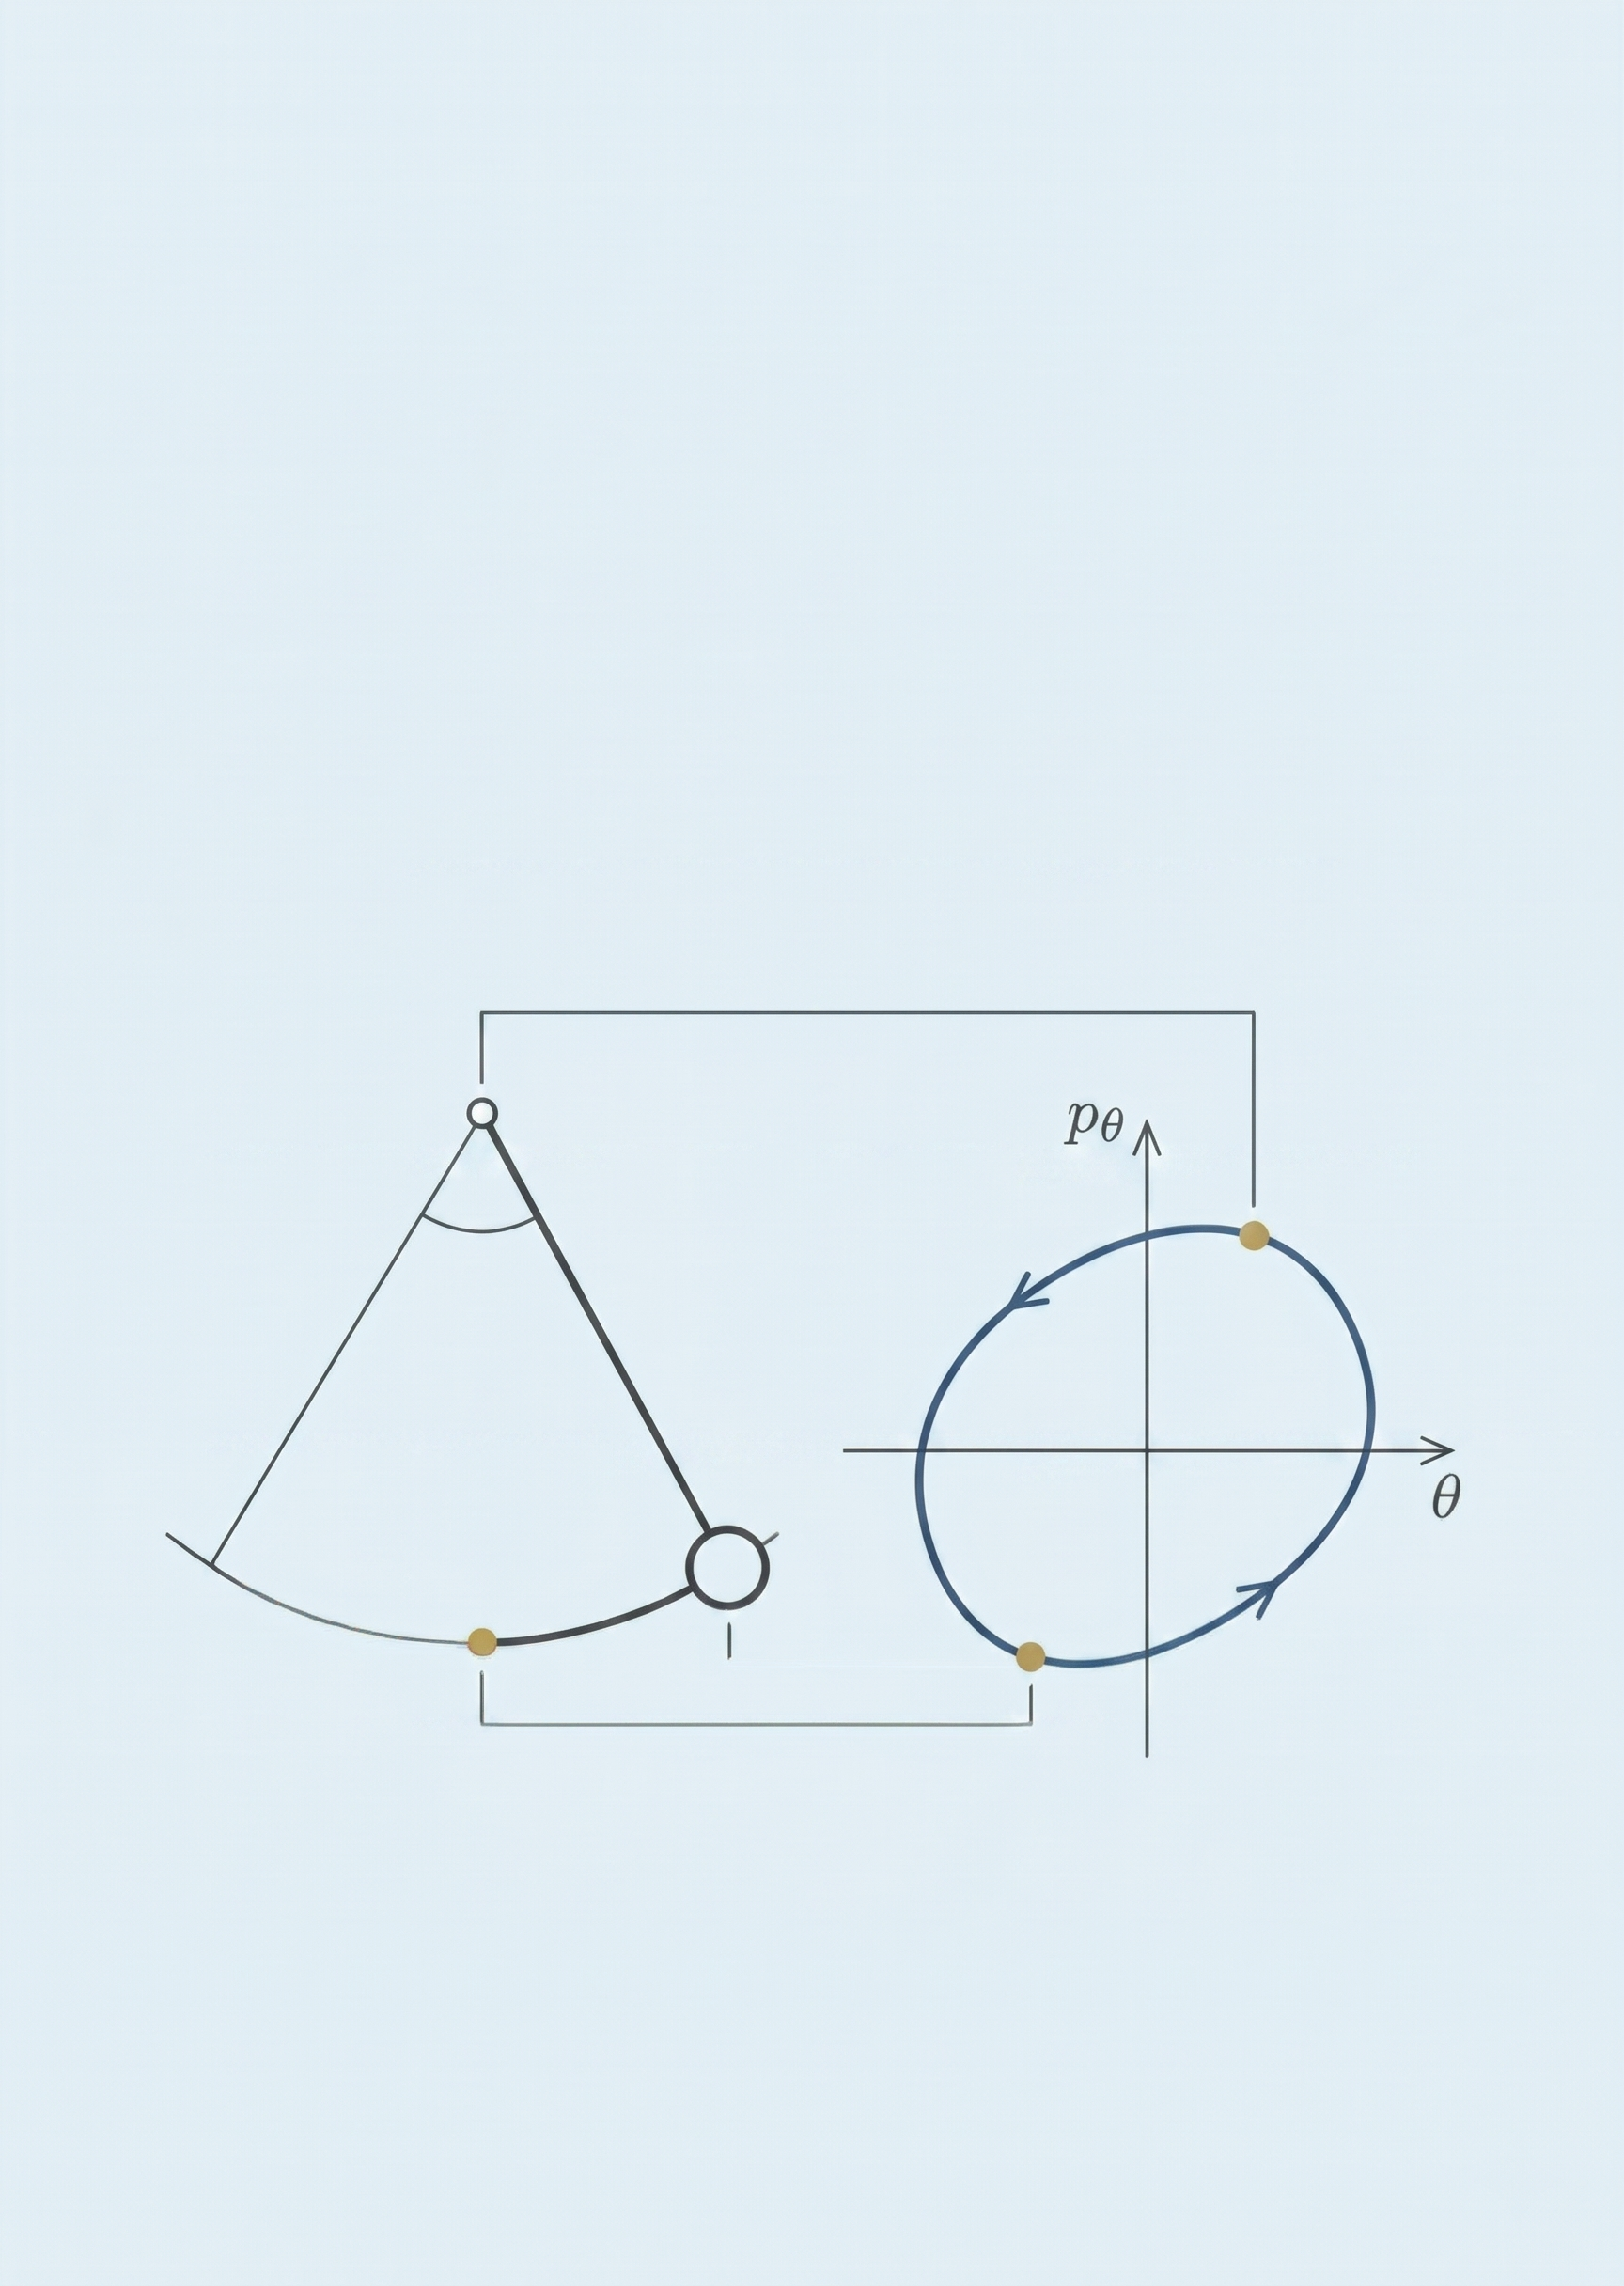
\includegraphics[height=\paperheight,keepaspectratio]{../../../generated_course_notes/core/classical_mechanics/2011_fall_theoretical_minimum/assets/cover-art.png}%
  };
  \node[
    anchor=north west,
    align=left,
    text width=0.78\paperwidth,
    fill=white,
    fill opacity=0.9,
    rounded corners=8pt,
    inner xsep=10pt,
    inner ysep=8pt
  ] at ([xshift=0.08\paperwidth,yshift=-0.06\paperheight]current page.north west) {%
    {\fontsize{30}{33}\selectfont\bfseries\color{black!88} Классическая механика\\[0.85em]}
    {\large\color{black!72} Русское издание / осень 2011, теоретический минимум}
  };
  \node[
    anchor=south west,
    align=left,
    text width=0.68\paperwidth,
    fill=white,
    fill opacity=0.82,
    text opacity=1,
    rounded corners=6pt,
    inner sep=12pt
  ] at ([xshift=0.08\paperwidth,yshift=0.08\paperheight]current page.south west) {%
    {\normalsize\color{black!78} Оригинальные лекции: Leonard Susskind\\[0.35em]}
    {\small\color{black!72} Сопроводительное издание: \href{https://lazying.art}{LazyingArt LLC} / \href{https://github.com/lachlanchen/Video2Book}{Video2Book}}
  };
\end{tikzpicture}
\mbox{}
\end{titlepage}
\hypersetup{pageanchor=true}

\clearpage
\chapter*{Об этих конспектах}
Эти независимо отредактированные сопроводительные конспекты составлены по лекциям Леонарда Сасскинда. Они были восстановлены по машинным расшифровкам, субтитрам и отобранным кадрам с доской, а затем сверены с доступными исходными материалами. Они не являются оригинальной рукописью профессора Сасскинда, не были им проверены и не получили его одобрения.

Издание подготовлено \href{https://lazying.art}{LazyingArt LLC} с использованием конвейера \href{https://github.com/lachlanchen/Video2Book}{Video2Book} с открытым исходным кодом. Машинные расшифровки по-прежнему доступны отдельно и могут содержать ошибки распознавания. Редакторские уточнения и нетривиальные реконструкции отмечены в сносках.
\clearpage
\tableofcontents
\mainmatter
\chapter{Состояния, обратимость и кинематика}

Классическая механика — это не только набор уравнений для падающих тел, обращающихся планет или заряженных частиц. Прежде чем выбирать какое-либо конкретное уравнение, можно задать более общий вопрос: каким должен быть закон движения, чтобы считаться классическим законом? Мы начнем с систем настолько простых, что любую возможную историю можно нарисовать на доске. Когда идеи состояния, детерминизма, обратимости и сохранения станут там ясны, мы вернемся к частицам, движущимся в обычном пространстве.

\section{Два вида вопросов}

В механике есть два вида вопросов. Один из них касается конкретного закона, управляющего данной системой. Планета, движущаяся в гравитационном поле массивного тела, подчиняется одному закону; электрически заряженная частица, движущаяся в магнитном поле, — другому. Это вопросы о детальных законах природы.

Другой вопрос касается структуры, общей для всех таких примеров. Существуют ли правила, которым должен удовлетворять всякий допустимый закон? Какие черты принадлежат самой классической механике, независимо от силы или объекта, который мы изучаем? Конкретные примеры проиллюстрируют ответ, но именно этот второй вопрос и организует предмет.

Самый полезный первый пример — абстрактная монета на абстрактном столе. Мы сохраняем только одно свойство монеты: она может показывать орла или решку. Поэтому ее пространство конфигураций равно
\begin{equation}
  \mathcal C=\{H,T\}.
\end{equation}
Слово \emph{конфигурация} означает один из возможных способов, которыми может быть устроена система. Начальное условие — это выбор одного из них. Односторонняя монета была бы еще проще, но у нее была бы только одна конфигурация, и ничего никогда не могло бы произойти. Двух состояний достаточно, чтобы динамика стала возможной.

\section{Монета: состояние, закон и история}

Пусть время идет целыми шагами, как если бы мир освещался стробоскопом:
\begin{equation}
  t=\ldots,-2,-1,0,1,2,\ldots .
\end{equation}
Закон движения — это правило обновления. Оно сопоставляет состоянию в момент \(t\) состояние в момент \(t+1\). Самое простое правило ничего не меняет:
\begin{equation}
  H\longmapsto H,
  \qquad
  T\longmapsto T.
  \label{eq:coin-identity}
\end{equation}
Если начать с \(H\), вся история имеет вид \(H,H,H,\ldots\); если начать с \(T\), она имеет вид \(T,T,T,\ldots\). Это правило скучно, но полностью определяет эволюцию.

Другое обратимое правило переставляет два состояния местами:
\begin{equation}
  H\longmapsto T,
  \qquad
  T\longmapsto H.
  \label{eq:coin-flip}
\end{equation}
Теперь истории чередуются:
\begin{equation}
  H,T,H,T,\ldots,
  \qquad
  T,H,T,H,\ldots .
\end{equation}
Стрелка указывает из состояния до обновления в состояние после него. Поэтому хвост стрелки показывает, с чего система начинает, а ее наконечник — куда она переходит.

\begin{figure}[htbp]
  \centering
  \includegraphics[width=0.86\textwidth]{lecture_01_figure_02.png}
  \caption{Две конфигурации монеты и ориентированный закон переворота на лекционной доске. Четкое правило обновления приведено в уравнении~\eqref{eq:coin-flip}.}
  \lectureframe{00:06:50}
  \label{fig:coin-board}
\end{figure}

Стороны можно закодировать двузначной переменной,
\begin{equation}
  \sigma=
  \begin{cases}
    +1,&H,\\
    -1,&T.
  \end{cases}
\end{equation}
Буква \(\sigma\) традиционно используется в физике для двузначных величин, особенно в описаниях спина, хотя никакого знания о спине здесь не требуется. В этих обозначениях два правила становятся уравнениями движения:
\begin{align}
  \sigma(t+1)&=\sigma(t),
  &&\text{identity law},\label{eq:sigma-identity}\\
  \sigma(t+1)&=-\sigma(t),
  &&\text{flip law}.\label{eq:sigma-flip}
\end{align}
Сама переменная не добавляет новой физики. Она дает компактную метку для конфигурации и превращает граф в уравнение.

\begin{figure}[htbp]
  \centering
  \includegraphics[width=0.86\textwidth]{lecture_01_figure_03.png}
  \caption{Закон переворота, записанный как
  \(\sigma(t+1)=-\sigma(t)\). Заключенные в рамку значения \(\sigma=\pm1\) обозначают орла и решку.}
  \lectureframe{00:08:58}
  \label{fig:sigma-board}
\end{figure}

Для любого из двух правил начальное состояние и закон определяют состояние в любой более поздний момент времени. Это утверждение предполагает, что система \emph{замкнута}. Если кто-то протянет руку и перевернет монету, то эта рука будет внешним воздействием, не включенным в наше описание. Мы не опровергли детерминизм; мы изменили систему. Классический закон предназначен управлять замкнутой системой, в описание которой включены все воздействия, существенные для ее эволюции.

Существует 4 математические функции из двухэлементного множества в себя. Те две, которые выше не записаны, сопоставляют обоим входам \(H\) либо обоим входам \(T\). Они однозначно задают будущее, но стирают различие между двумя возможными прошлыми. Когда ниже будет наложено требование обратимости, уравнения~\eqref{eq:coin-identity} и \eqref{eq:coin-flip} окажутся в точности двумя допустимыми отображениями.

\section{Игральная кость: орбиты и сохраняющиеся величины}

Заменим монету игральной костью. Для наших целей важен лишь один факт об игральной кости: у нее 6 конфигураций,
\begin{equation}
  \mathcal C=\{1,2,3,4,5,6\}.
\end{equation}
Начальное условие — это выбор одного числа. Мы снова могли бы оставить каждое состояние неподвижным, но ориентированные графы полезнее для менее тривиальных правил. Рассмотрим
\begin{equation}
  1\longmapsto2\longmapsto3\longmapsto4
  \longmapsto5\longmapsto6\longmapsto1.
  \label{eq:six-cycle}
\end{equation}
Если, например, начать с \(4\), то история будет такой

\[
  4,5,6,1,2,3,4,\ldots .
\]
Шесть состояний образуют один цикл.\footnote{Примечание к источнику: при первом чтении стрелок в одной устной фразе говорится, что \(6\) возвращается в \(6\). Сразу следующая фраза, нарисованный цикл и перечисленная история все указывают на подразумеваемый переход \(6\mapsto1\).}

\begin{figure}[htbp]
  \centering
  \includegraphics[width=0.86\textwidth]{lecture_01_figure_06.png}
  \caption{Единственный цикл из 6 состояний. При каждом стробоскопическом шаге состояние переходит в следующее и возвращается после 6 обновлений.}
  \lectureframe{00:12:40}
  \label{fig:six-cycle-board}
\end{figure}

Правило может выглядеть сложнее, не будучи структурно иным. Например,
\begin{equation}
  1\to2\to5\to3\to4\to6\to1
  \label{eq:relabeled-cycle}
\end{equation}
это по-прежнему один цикл длины 6. Если расположить вершины на странице в порядке \(1,2,5,3,4,6\), получится та же схема, что и в уравнении~\eqref{eq:six-cycle}. Метки вроде \(1\) и \(5\) — это имена; структура цикла от них не зависит.

По-настоящему другой закон разбивает 6 состояний на 2 цикла, например
\begin{equation}
  1\to2\to3\to1,
  \qquad
  4\to6\to5\to4.
  \label{eq:two-cycles}
\end{equation}
Игральная кость по-прежнему одна и закон один, но траектория, которая начинается на одном цикле, никогда не может попасть на другой. Можно приписать циклам число \(Q\),
\begin{equation}
  Q=
  \begin{cases}
    0,&\text{on the cycle }\{1,2,3\},\\
    1,&\text{on the cycle }\{4,5,6\}.
  \end{cases}
\end{equation}
Состояние меняется на каждом шаге, а \(Q\) — нет.

\begin{definition}
Сохраняющаяся величина — это функция состояния, значение которой не изменяется под действием закона движения.
\end{definition}

Та же идея допускает одну неподвижную точку, один двухцикл и один трехцикл. Сохраняющаяся метка указывает, на какой орбите находится система; она не обязана определять состояние внутри этой орбиты. Таким образом, сохранение совместимо с движением. Сохраняется не обязательно полная конфигурация, а некоторое различие между возможными конфигурациями.

\begin{figure}[htbp]
  \centering
  \includegraphics[width=0.86\textwidth]{lecture_01_figure_07.png}
  \caption{Несколько несвязанных циклов на доске: неподвижная точка, двухцикл и трехцикл. Метка цикла сохраняется даже тогда, когда состояние движется по своему циклу.}
  \lectureframe{00:18:40}
  \label{fig:conserved-cycles-board}
\end{figure}

В конечной обратимой системе всякая траектория является циклом. У единственного цикла нет непостоянной сохраняющейся метки такого элементарного вида, потому что траектория рано или поздно проходит через каждое состояние. Несколько циклов допускают такую метку, поскольку эволюция никогда не переносит состояние из одной компоненты в другую.

\section{Что должно входить в состояние?}

В примерах с монетой использовалось одношаговое правило: следующая сторона зависела только от текущей стороны. Вопрос из аудитории проверяет, существенно ли это ограничение.

\begin{classroomqa}
\audiencequestion{Можно ли построить последовательность орлов и решек, в которой следующий результат зависит не только от непосредственно видимой стороны, а, возможно, от одного или нескольких предыдущих результатов?\lecturetimestamp{00:19:27--00:21:23}}

\lecturerresponse{Да. В этом случае одних \(H\) или \(T\) недостаточно для полного задания состояния. Если нужна одна предыдущая сторона, расширьте пространство состояний до
\(
  \{HH,HT,TH,TT\}.
\)
Каждая упорядоченная пара записывает текущую сторону и предыдущую. Тогда эволюцию снова можно записать как одношаговое правило на этом пространстве из четырех состояний. Если требуется еще больше предыстории, включите и эту информацию.}
\end{classroomqa}

Этот ответ дает операциональный смысл состояния.

\begin{definition}
Состояние системы в некоторый момент состоит из всей информации, необходимой вместе с законом движения для предсказания ее будущего.
\end{definition}

Следовательно, состояние — не просто фотография. Это любой полный набор данных, делающий эволюцию однозначной. Позже, когда мы будем описывать ньютоновскую частицу, одного ее положения будет недостаточно; к начальным данным будет относиться и скорость. Монета с памятью — простейший вариант того же принципа.

\section{Бесконечные пространства состояний}

Бесконечное число состояний не требует бесконечного числа объектов. Рассмотрим одну частицу, ограниченную целочисленными узлами бесконечной прямой. Ее состояние задается целым числом
\[
  n\in\mathbb Z.
\]
Один закон сдвигает ее на один узел вправо на каждом шаге:
\begin{equation}
  n(t+1)=n(t)+1.
  \label{eq:lattice-one}
\end{equation}
Эта орбита никогда не замыкается, но проходит через каждое целое число, если проследить ее как в будущее, так и в прошлое. В этом расширенном смысле она играет роль одного бесконечного цикла.

Другой закон сдвигает ее сразу на два узла:
\begin{equation}
  n(t+1)=n(t)+2.
  \label{eq:lattice-two}
\end{equation}
Теперь четные узлы переходят только в четные, а нечетные — только в нечетные. Четность сохраняется:
\begin{equation}
  \begin{aligned}
    Q_{\rm parity}(n)&=n\bmod 2,\\
    Q_{\rm parity}(n(t+1))&=Q_{\rm parity}(n(t)).
  \end{aligned}
\end{equation}
Переход от конечного пространства конфигураций к бесконечному допускает истории, которые никогда не повторяются, но не меняет смысла понятий состояния, орбиты или сохранения.

\section{Детерминизм — это еще не обратимость}

Теперь введем правило, которое однозначно предсказывает будущее, но не удовлетворяет второму классическому требованию. Припишем трехсторонней монете состояния орел, решка и ребро и определим
\begin{equation}
  H\to T,
  \qquad
  T\to E,
  \qquad
  E\to T.
  \label{eq:nonreversible-map}
\end{equation}
Начиная с \(H\), история имеет вид
\[
  H,T,E,T,E,\ldots;
\]
а начиная либо с \(T\), либо с \(E\), последующее чередование столь же однозначно. Из каждого состояния выходит ровно одна стрелка, так что это правило детерминистично по отношению к будущему.

Трудность возникает, когда мы пытаемся восстановить прошлое. Если текущее состояние — \(T\), то предыдущим могло быть \(H\) или \(E\). Две истории слились. Если обратить каждую стрелку, изъян сразу становится очевидным: из \(T\) на обращенном графе возможны два хода. Обратное правило не является детерминистическим.

\begin{figure}[htbp]
  \centering
  \includegraphics[width=0.86\textwidth]{lecture_01_figure_08.png}
  \caption{Необратимый закон для \(H,T,E\) и характерные истории. И \(H\), и \(E\) переходят в \(T\), так что настоящее не определяет единственного прошлого.}
  \lectureframe{00:28:50}
  \label{fig:nonreversible-board}
\end{figure}

\begin{definition}
Дискретный закон обратим, если текущее состояние определяет как единственное следующее состояние, так и единственное предыдущее состояние. В графе состояний из каждого состояния должна выходить ровно одна стрелка и в него должна входить ровно одна стрелка.
\end{definition}

Для конечного пространства состояний обратимое обновление представляет собой перестановку состояний. Оно никогда не создает и не уничтожает различий между состояниями; оно лишь переставляет их. Поэтому его граф распадается на циклы. Отображение в уравнении~\eqref{eq:nonreversible-map} является функцией, но не взаимно однозначной функцией, и потому не имеет обратного отображения.

\begin{classroomqa}
\audiencequestion{Могло бы правило такого рода быть допустимым, если бы состояния представляли вероятности для частицы?\lecturetimestamp{00:29:46--00:31:17}}

\lecturerresponse{Это была бы другая схема. Фундаментальная классическая механика в той формулировке, которую мы здесь используем, опирается на детерминистические законы, а не на вероятностные правила обновления. Конечно, такое правило можно придумать и изучать, но в этом смысле оно не является законом классической механики. Квантовая механика не детерминистична в том же смысле и тем не менее имеет аналог обратимой эволюции; это требует отдельного, более позднего обсуждения. Классическая статистическая механика тоже использует вероятности, но она исходит из лежащих в основе механических законов и описывает неполное знание о начальных данных.}
\end{classroomqa}

Это различие важно. Распределение вероятностей, используемое потому, что мы не знаем точного классического состояния, не является индетерминистическим законом движения. Оно описывает нашу информацию о системе, микроскопическая эволюция которой по-прежнему считается детерминистической и обратимой.

\section{Точные законы и неполное знание}

Для предсказания требуются две составляющие:
\begin{enumerate}
  \item закон движения;
  \item начальное состояние.
\end{enumerate}
Точный закон не дает точного прогноза, если начальное условие известно лишь приблизительно. Для монеты легко представить, что мы смотрим на стол и совершенно точно узнаем, какой стороной она лежит. Реальные механические переменные непрерывны. Положения и скорости могут принимать произвольные вещественные значения, и никакое измерение не дает бесконечно много десятичных знаков.

Предположим, что истинное начальное состояние лежит в небольшой области возможных состояний. При одной динамике эта область долго остается небольшой; при другой близкие начальные состояния быстро расходятся. В хаотической системе малые начальные неопределенности со временем вырастают в большие различия. Атмосфера — хорошо известный пример. Более точные измерения могут продлить интервал полезного прогноза, но при любой фиксированной точности измерения найдется достаточно удаленный момент времени, в который прогноз становится ненадежным.

Это практическое ограничение не вносит неоднозначности в уравнения. Если бы начальные условия были известны точно, классический обратимый закон определял бы и будущее, и прошлое. При конечной точности количественный вопрос вместо этого таков: насколько точно должно быть известно начальное состояние, чтобы сделать предсказание на заданный промежуток времени?

Теперь графический критерий приводит к краткому выводу. Закон, представленный одной входящей и одной исходящей стрелкой в каждом состоянии, детерминистичен и обратим. Соответствующие утверждения для частиц будут менее элементарны, но они выражают ту же классическую структуру.

\section{От абстрактных состояний к точкам в пространстве}

Теперь мы переходим от монет и игральных костей к материальным точкам. Материальная точка может двигаться в одном, трех, пяти или любом другом числе измерений, но непосредственный пример дает обычное пространство. Чтобы количественно задать точку, выберите:
\begin{itemize}
  \item начало координат;
  \item три взаимно перпендикулярные оси;
  \item ориентацию этих осей;
  \item единицу длины.
\end{itemize}
Начало координат выбирается условно. Его можно поместить в Пало-Альто или где угодно еще, и физические выводы не должны зависеть от этого выбора. Оси можно обозначить как \(x,y,z\) или как \(x_1,x_2,x_3\). После того как направления \(x\) и \(y\) зафиксированы, ось \(z\) может быть направлена в любое из двух направлений, перпендикулярных им обоим. Мы выбираем правостороннюю конвенцию: если большой палец правой руки направлен вдоль \(x\), а указательный — вдоль \(y\), то средний палец указывает вдоль \(z\).

Чтобы наносить равные отметки вдоль осей, нужна единица длины, например метры, футы, дюймы или световые годы. После того как эти соглашения зафиксированы, каждая точка задается тремя числами,
\begin{equation}
  (x,y,z).
\end{equation}
В точку можно попасть из начала координат, смещаясь вдоль трех осей. Система из многих частиц требует по одной такой тройке для каждой частицы.

\begin{figure}[htbp]
  \centering
  \includegraphics[width=0.86\textwidth]{lecture_01_figure_09.png}
  \caption{Декартовы оси и три координаты точки. Рисунок фиксирует координатное соглашение; сама точка не зависит от того, где мы выбираем начало координат или оси.}
  \lectureframe{00:43:00}
  \label{fig:coordinates-board}
\end{figure}

\section{Векторы и их компоненты}

Вектор — это объект, имеющий величину и направление. Перемещение от начала координат к точке есть вектор, но векторы также описывают скорость, ускорение, электрические поля и многие другие величины. Мы будем обозначать вектор полужирным шрифтом, например \(\mathbf v\), а его модуль — как \(\lvert\mathbf v\rvert\). Модуль неотрицателен и обращается в нуль только для нулевого вектора.

С геометрической точки зрения вектор — это свободная стрелка. Параллельный перенос стрелки без изменения ее длины или направления не изменяет вектор. В конкретном приложении вектор может быть привязан к точке, например когда мы задаем электрическое поле в данной точке, но такая привязка является дополнительной информацией и не входит в само абстрактное понятие вектора.

Относительно декартовых осей вектор имеет компоненты
\begin{equation}
  \mathbf v=(v_x,v_y,v_z).
\end{equation}
Компоненты — это обычные числа со знаком, получаемые проецированием на оси. Они задают и величину, и направление. Трехмерная теорема Пифагора дает
\begin{equation}
  \lvert\mathbf v\rvert^2
  =v_x^2+v_y^2+v_z^2,
  \qquad
  \lvert\mathbf v\rvert
  =\sqrt{v_x^2+v_y^2+v_z^2}.
  \label{eq:vector-magnitude}
\end{equation}
Отношения компонент определяют направление. Отрицательная компонента означает, что вектор отчасти направлен вдоль отрицательного направления соответствующей оси.

\subsection{Умножение на скаляр и сложение}

Умножение на вещественное число изменяет длину вектора и, если это число отрицательно, меняет его направление на противоположное. При \(c>0\) вектор \(c\mathbf A\) направлен так же, как \(\mathbf A\), и имеет модуль \(c\lvert\mathbf A\rvert\). В частности, \(-\mathbf A\) имеет ту же длину, что и \(\mathbf A\), и направлен противоположно.

Есть три эквивалентных наглядных представления сложения векторов. Во-первых, поместите начало \(\mathbf B\) в конец \(\mathbf A\); стрелка от начала \(\mathbf A\) к концу \(\mathbf B\) есть \(\mathbf A+\mathbf B\). Во-вторых, совместите оба начала и достройте параллелограмм; его диагональ и есть сумма. В этой форме наглядно видна коммутативность:
\begin{equation}
  \mathbf A+\mathbf B=\mathbf B+\mathbf A.
\end{equation}
В-третьих, сложите соответствующие компоненты:
\begin{equation}
  C_i=A_i+B_i,
  \qquad i=x,y,z,
  \label{eq:component-addition}
\end{equation}
где \(\mathbf C=\mathbf A+\mathbf B\). Эти правила также определяют произвольные линейные комбинации, такие как \(a\mathbf A+b\mathbf B\).

\begin{figure}[htbp]
  \centering
  \includegraphics[width=0.86\textwidth]{lecture_01_figure_10.png}
  \caption{Треугольное и параллелограммное построения для сложения векторов. Оба дают один и тот же вектор \(\mathbf A+\mathbf B\).}
  \lectureframe{00:53:00}
  \label{fig:vector-addition-board}
\end{figure}

Общей операции деления одного вектора на другой не существует. Однако существуют два стандартных произведения векторов. Векторное произведение мы оставим для более поздней лекции. Здесь нам нужно скалярное произведение.

\subsection{Скалярное произведение}

Спроецируйте \(\mathbf A\) на ось, задаваемую \(\mathbf B\). Если угол между векторами равен \(\theta\), то алгебраическая компонента \(\mathbf A\) вдоль \(\mathbf B\) равна \(\lvert\mathbf A\rvert\cos\theta\). Умножение этой проекции на \(\lvert\mathbf B\rvert\) определяет
\begin{equation}
  \mathbf A\cdot\mathbf B
  =\lvert\mathbf A\rvert\,\lvert\mathbf B\rvert\cos\theta.
  \label{eq:dot-geometric}
\end{equation}
Результат — скаляр, а не еще один вектор. Уравнение~\eqref{eq:dot-geometric} симметрично относительно \(\mathbf A\) и \(\mathbf B\), так что \(\mathbf A\cdot\mathbf B=\mathbf B\cdot\mathbf A\).

\begin{figure}[htbp]
  \centering
  \includegraphics[width=0.86\textwidth]{lecture_01_figure_11.png}
  \caption{Построение скалярного произведения на доске с помощью проекции. В печатной записи это
  \(\mathbf A\cdot\mathbf B=AB\cos\theta\).}
  \lectureframe{00:58:30}
  \label{fig:dot-product-board}
\end{figure}

Знак несет геометрическую информацию. Скалярное произведение положительно при остром угле, отрицательно при тупом и равно нулю для перпендикулярных векторов. Следовательно,
\begin{equation}
  \mathbf A\perp\mathbf B
  \quad\Longleftrightarrow\quad
  \mathbf A\cdot\mathbf B=0
\end{equation}
для ненулевых векторов.

В компонентах,
\begin{equation}
  \mathbf A\cdot\mathbf B
  =A_xB_x+A_yB_y+A_zB_z.
  \label{eq:dot-components}
\end{equation}
эта формула позволяет выполнять вычисления сразу. В частности,
\begin{equation}
  \mathbf A\cdot\mathbf A
  =A_x^2+A_y^2+A_z^2
  =\lvert\mathbf A\rvert^2.
  \label{eq:self-dot}
\end{equation}
Если заданы компоненты двух векторов, то формулы~\eqref{eq:dot-geometric} и
\eqref{eq:dot-components} определяют угол между ними:
\begin{equation}
  \cos\theta
  =\frac{\mathbf A\cdot\mathbf B}
  {\lvert\mathbf A\rvert\,\lvert\mathbf B\rvert}.
\end{equation}

Закон косинусов следует из той же алгебры. Пусть \(\mathbf A\) и
\(\mathbf B\) проведены из одной вершины к двум другим вершинам треугольника.
Третья сторона есть
\(\mathbf C=\mathbf A-\mathbf B\), а не \(\mathbf A+\mathbf B\). Поэтому
\begin{align}
  C^2
  &=(\mathbf A-\mathbf B)\cdot(\mathbf A-\mathbf B)\notag\\
  &=A^2+B^2-2\mathbf A\cdot\mathbf B\notag\\
  &=A^2+B^2-2AB\cos\theta.
  \label{eq:law-of-cosines}
\end{align}

\begin{figure}[htbp]
  \centering
  \includegraphics[width=0.86\textwidth]{lecture_01_figure_04.png}
  \caption{Треугольник, используемый для закона косинусов. Исправление на доске
  показывает, что замыкающая сторона равна
  \(\mathbf C=\mathbf A-\mathbf B\), что приводит к
  формуле~\eqref{eq:law-of-cosines}.}
  \lectureframe{01:04:29}
  \label{fig:law-cosines-board}
\end{figure}

\section{Положение, скорость и ускорение}

Выберем начало координат, и пусть \(\mathbf r\) — радиус-вектор, проведенный от него
к частице. Его компоненты — декартовы координаты:
\begin{equation}
  \mathbf r=(x,y,z),
  \qquad
  \lvert\mathbf r\rvert=\sqrt{x^2+y^2+z^2}.
\end{equation}
Изменение этого выбора меняет \(\mathbf r\); к этому вопросу мы пока вернемся позже. Когда
оно зафиксировано, движение описывается зависящим от времени положением,
\begin{equation}
  \mathbf r(t)=\bigl(x(t),y(t),z(t)\bigr).
\end{equation}
Следовательно, траектория задается тремя функциями времени.

Скорость есть производная положения по времени:
\begin{equation}
  \mathbf v(t)=\frac{d\mathbf r}{dt}
  =\dot{\mathbf r}(t),
  \qquad
  v_i=\frac{dx_i}{dt}=\dot x_i.
  \label{eq:velocity}
\end{equation}
Точка сверху всегда обозначает производную по времени. Величина
\(\lvert\mathbf v\rvert\) есть модуль скорости. В общем случае направления радиус-вектора и
скорости независимы: частица, находящаяся в данной точке, может двигаться в любом
направлении, допускаемом задачей.

Ускорение есть скорость изменения скорости и, следовательно, вторая производная
положения по времени:
\begin{equation}
  \mathbf a(t)=\frac{d\mathbf v}{dt}
  =\dot{\mathbf v}(t)
  =\frac{d^2\mathbf r}{dt^2}
  =\ddot{\mathbf r}(t),
  \qquad
  a_i=\ddot x_i.
  \label{eq:acceleration}
\end{equation}
Ускорение тоже является вектором. Если частица, движущаяся в положительном
направлении \(x\), увеличивает скорость, то \(a_x>0\). Если она замедляется, то \(a_x<0\). То, что
часто называют замедлением, — это просто ускорение, направленное противоположно текущей
скорости. В более общем случае скорость может изменяться за счет изменения своего направления
даже тогда, когда ее величина остается постоянной.

\begin{figure}[htbp]
  \centering
  \includegraphics[width=0.86\textwidth]{lecture_01_figure_05.png}
  \caption{Компоненты скорости, записанные как производные по времени от компонент
  положения. В компактной векторной записи,
  \(\mathbf v=d\mathbf r/dt\).}
  \lectureframe{01:14:24}
  \label{fig:velocity-board}
\end{figure}

\subsection{Движение на прямой с постоянным ускорением}

Для одномерного движения запишем
\begin{equation}
  x(t)=a+bt+ct^2.
  \label{eq:quadratic-motion}
\end{equation}
При \(t=0\) частица находится в \(x=a\). Однократное, а затем двукратное
diфференцирование дает
\begin{align}
  v(t)=\dot x(t)&=b+2ct,\label{eq:line-velocity}\\
  a(t)=\ddot x(t)&=2c.\label{eq:line-acceleration}
\end{align}
Следовательно, \(b\) — это начальная скорость, а \(2c\) — постоянное ускорение. Если
\(c>0\), скорость линейно возрастает; если \(c<0\), она линейно убывает.
Этот квадратичный закон положения — именно та форма, которую принимает движение при постоянном
ускорении, например идеализированное движение падающего тела вблизи поверхности
Земли.

\section{Равномерное движение по окружности}

В качестве последнего примера пусть частица движется в плоскости \(x\)-\(y\) по
единичной окружности. При \(t=0\) она находится на положительной полуоси \(x\), а ее угловая
координата растет равномерно:
\begin{equation}
  \theta(t)=\omega t.
\end{equation}
Постоянная \(\omega\) есть угловая частота. Одному обороту соответствует
увеличение угла на \(2\pi\), поэтому период равен
\begin{equation}
  T=\frac{2\pi}{\omega}.
  \label{eq:circular-period}
\end{equation}
Можно позволить углу возрастать и дальше \(2\pi\); положение повторяется,
хотя непрерывно отслеживаемый угол не сбрасывается.

На единичной окружности,
\begin{equation}
  \mathbf r(t)
  =\bigl(\cos\omega t,\,\sin\omega t\bigr).
  \label{eq:circular-position}
\end{equation}
Дифференцирование дает
\begin{equation}
  \mathbf v(t)
  =\omega\bigl(-\sin\omega t,\,\cos\omega t\bigr).
  \label{eq:circular-velocity}
\end{equation}
Скорость направлена по касательной к окружности. Ее перпендикулярность
радиусу можно доказать, не опираясь на рисунок:
\begin{align}
  \mathbf r\cdot\mathbf v
  &=\cos\omega t\,(-\omega\sin\omega t)
    +\sin\omega t\,(\omega\cos\omega t)\notag\\
  &=0.
  \label{eq:r-dot-v}
\end{align}

\begin{figure}[htbp]
  \centering
  \includegraphics[width=0.86\textwidth]{lecture_01_figure_12.png}
  \caption{Компоненты положения и скорости при движении по единичной окружности.
  Сокращение в \(\mathbf r\cdot\mathbf v\) показывает, что скорость
  направлена по касательной к окружности.}
  \lectureframe{01:24:30}
  \label{fig:circular-velocity-board}
\end{figure}

Дифференцируя еще раз,
\begin{equation}
  \mathbf a(t)
  =-\omega^2
  \bigl(\cos\omega t,\,\sin\omega t\bigr)
  =-\omega^2\mathbf r(t).
  \label{eq:centripetal-acceleration}
\end{equation}
Ускорение параллельно радиусу, но направлено в противоположную
сторону, к центру. Это центростремительное ускорение.\footnote{Терминологическое
замечание: в этом месте лекции встречается слово ``центробежное'', но
уравнение и сопровождающее описание указывают на стандартное центростремительное
ускорение, направленное к центру.}

\begin{figure}[H]
  \centering
  \includegraphics[width=0.86\textwidth]{lecture_01_figure_13.png}
  \caption{Покомпонентное вычисление ускорения при движении по окружности. Каждая
  компонента равна соответствующей компоненте положения, умноженной на \(-\omega^2\), поэтому
  \(\mathbf a=-\omega^2\mathbf r\).}
  \lectureframe{01:26:30}
  \label{fig:circular-acceleration-board}
\end{figure}

Поскольку радиус равен единице,
\begin{equation}
  \lvert\mathbf r\rvert=1,
  \qquad
  \lvert\mathbf v\rvert=\omega,
  \qquad
  \lvert\mathbf a\rvert=\omega^2.
\end{equation}
При увеличении \(\omega\) модуль скорости растет линейно, а требуемое направленное внутрь
ускорение — квадратично. Для окружности радиуса \(R\) тот же расчет
дал бы \(v=\omega R\) и
\(\lvert\mathbf a\rvert=\omega^2R=v^2/R\); в лекции используется \(R=1\), чтобы не загромождать
первое вычисление.

Теперь у нас есть элементарный язык, необходимый для механики частицы: состояния и
начальные данные, обратимая эволюция, координаты, векторы и производные,
определяющие скорость и ускорение. Следующая задача состоит в том, чтобы точно
определить, какие начальные данные нужно задать для частицы, и найти законы,
которые переносят эти данные от одного момента к следующему.

\chapter{Силы, фазовое пространство и законы сохранения}

\lectureoverview{Закон движения должен делать больше, чем просто связывать знакомые физические величины. Он должен задавать состояние системы, переводить это состояние от одного момента к следующему и показывать, какие различия и какие величины сохраняются при движении. Мы придём к ньютоновской механике, сначала проверив правдоподобный, но неверный закон силы, затем расширив описание состояния от положения до фазового пространства и, наконец, выведя законы сохранения импульса и энергии.}

\section{Полезный неверный закон}

В повседневном движении доминирует трение. Если толкать тяжёлый предмет по полу, он движется; если перестать толкать, он вскоре останавливается. Большее усилие обычно даёт большую скорость, тогда как более тяжёлый предмет требует большего усилия. В таком мире естественно предположить, что сила порождает саму скорость. Именно на этой интуиции основывалось аристотелевское описание движения.

Катание на коньках даёт недостающий опыт. Конькобежцу нужна сила, чтобы начать движение, остановиться или изменить направление, но не для того, чтобы, начав двигаться, продолжать скользить. Если бы Аристотель имел дело с почти лишённым трения льдом, а не с обычной землёй, не заметить изъян в представлении сила--скорость было бы гораздо труднее.

Чтобы выявить, что именно неверно в этой интуиции, придадим ей точную современную форму. Запишем заведомо неверное уравнение

\begin{equation}
  \mathbf F=m\mathbf v.
  \label{eq:aristotle-vector-law}
\end{equation}

Это не закон Ньютона, и его не следует заучивать как физику. Его ценность диагностическая: как только словесное правило превращено в уравнение, можно спросить, предсказывает ли оно движение и сохраняет ли достаточно информации, чтобы восстановить прошлое. Краткое обсуждение на занятии греческого слова для силы отсылает к \emph{dynamis}, корню, который слышен также в словах динамо и динамика, но терминология вторична по сравнению с проверкой самого закона.

\begin{figure}[htbp]
  \centering
  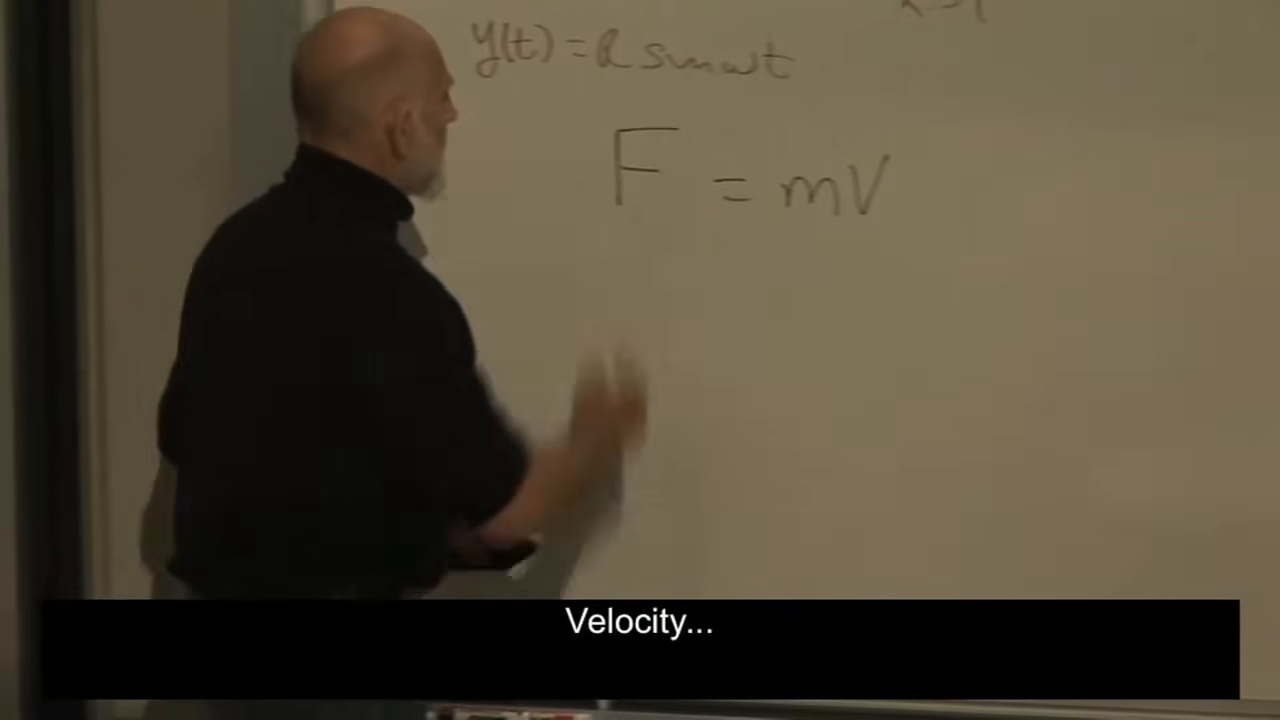
\includegraphics[width=0.82\textwidth]{lecture_02_figure_02.png}
  \caption{Намеренно неверный закон сила--скорость, используемый для проверки предсказуемости и обратимости.}
  \lectureframe{00:04:51}
\end{figure}

Ограничим движение одной пространственной координатой. Поскольку \(v=\dot x\), закон принимает вид

\begin{equation}
  F(t)=m\dot x(t).
  \label{eq:aristotle-1d}
\end{equation}

Теперь разобьём время на короткие интервалы длины \(\delta\). За один такой интервал,

\begin{equation}
  \dot x(t)\simeq
  \frac{x(t+\delta)-x(t)}{\delta}.
  \label{eq:first-difference}
\end{equation}

Подстановка в уравнение~\eqref{eq:aristotle-1d} даёт

\begin{equation}
  x(t+\delta)
  =x(t)+\frac{\delta}{m}F(t).
  \label{eq:aristotle-update}
\end{equation}

Это действительно имеет вид правила обновления. Если известны текущее положение и сила, то положение в следующий стробоскопический момент определяется однозначно. Однако когда сила исчезает, правило Аристотеля даёт \(\dot x=0\): объект должен оставаться в покое. Движение без поддерживающей силы исключается с самого начала.

\begin{figure}[htbp]
  \centering
  \includegraphics[width=0.84\textwidth]{lecture_02_figure_07.png}
  \caption{Дискретное обновление Аристотеля для случая возвращающей силы. На каждом шаге смещение умножается на множитель, немного меньший единицы.}
  \lectureframe{00:10:15}
\end{figure}

\subsection{Пружина в механике Аристотеля}

Рассмотрим частицу, прикреплённую к пружине, с положением равновесия при \(x=0\). Смещение создаёт возвращающую силу

\begin{equation}
  F(x)=-kx,
  \qquad k>0.
  \label{eq:hooke-law}
\end{equation}

Подставляя эту силу в уравнение~\eqref{eq:aristotle-update}, получаем

\begin{equation}
  x(t+\delta)
  =\left(1-\frac{k\delta}{m}\right)x(t).
  \label{eq:aristotle-spring-update}
\end{equation}

При достаточно малом \(\delta\) множитель в скобках оказывается чуть меньше единицы. Поэтому каждое обновление уменьшает смещение на одну и ту же долю:

\begin{equation}
  x_n=\left(1-\frac{k\delta}{m}\right)^n x_0.
  \label{eq:aristotle-geometric-decay}
\end{equation}

Непрерывное уравнение и его решение имеют вид

\begin{align}
  m\dot x&=-kx,
  \label{eq:aristotle-spring-continuous}\\
  x(t)&=x(0)e^{-kt/m}.
  \label{eq:aristotle-spring-solution}
\end{align}

Пружина не совершает колебаний. После освобождения из любого смещённого положения частица экспоненциально приближается к началу координат, двигаясь всё медленнее по мере приближения.

\begin{figure}[htbp]
  \centering
  \includegraphics[width=0.84\textwidth]{lecture_02_figure_08.png}
  \caption{Экспоненциальное решение уравнения пружины в механике Аристотеля. Смещение затухает, а не колеблется.}
  \lectureframe{00:12:02}
\end{figure}

Будущее предсказать легко: всякое начальное смещение приближается к одному и тому же состоянию покоя. С прошлым дело обстоит иначе. Предположим, что частица наблюдается очень близко к началу координат и лишь с конечной точностью. Она могла начинать с любого из многих различных смещений, поскольку все их экспоненциально малые остатки в конце концов попадают в один и тот же допуск измерения. При идеальной математической точности уравнение~\eqref{eq:aristotle-spring-solution} можно обратить по времени, но практические различия между историями неуклонно стираются. Поэтому этот закон подозрителен с точки зрения обратимой фундаментальной динамики.

Это не означает, что Аристотель был неразумен. Описанное им движение, в котором доминирует трение, действительно диссипативно. Ошибкой было возвести это эффективное поведение в ранг фундаментального закона. Само трение есть сила, возникающая из сложных микроскопических взаимодействий. Когда рука толкает тело с приблизительно постоянной скоростью, приложенная сила уравновешивает трение; приложенная сила как таковая не создаёт скорость.

\section{Закон Ньютона и его физический смысл}

Ньютоновская поправка состоит в том, что сила изменяет движение:

\begin{equation}
  \mathbf F=m\mathbf a=m\ddot{\mathbf x}.
  \label{eq:newton-second-law}
\end{equation}

Прежде чем рассматривать это как уравнение эволюции, надо распутать два кажущихся логических круга. Первый касается систем отсчёта. Часто говорят, что законы Ньютона выполняются в инерциальных системах отсчёта, а инерциальная система отсчёта — это такая система, в которой выполняются законы Ньютона. Физическое утверждение состоит не в этом циклическом определении. Оно состоит в эмпирическом утверждении, что \emph{существуют} системы отсчёта, задаваемые подходящими линейками и часами, в которых законы Ньютона принимают свой простой вид. В системах, ускоряющихся или вращающихся относительно них, необходимы дополнительные фиктивные силы. То, как уравнения преобразуются в этих других системах, можно выяснить позже.

Второй логический круг касается силы и массы. Если силу определить как произведение массы на ускорение, а массу — как силу, делённую на ускорение, уравнение кажется пустым. Операциональный эксперимент отделяет определения от закона. Сравните тело с эталонным килограммом, уравновесив их, а затем присоедините это тело к пружинному динамометру в пространстве, где в остальном силы отсутствуют. За одну единицу силы примем фиксированное малое удлинение пружины. Две одинаковые пружины, каждая растянутая на ту же величину, дают две единицы силы и создают вдвое большее ускорение. Добавить вторую пружину надёжнее, чем растянуть одну пружину вдвое сильнее, потому что реальная пружина в конце концов становится нелинейной или рвётся. Если оставить одну пружину, но соединить две равные массы, ускорение будет вдвое меньше; для трёх равных масс — втрое меньше.

\begin{figure}[htbp]
  \centering
  \includegraphics[width=0.84\textwidth]{lecture_02_figure_09.png}
  \caption{Мысленный эксперимент с пружинным динамометром, используемый для задания равных единиц силы и проверки пропорциональности ускорения силе.}
  \lectureframe{00:22:45}
\end{figure}

Эти сравнения придают эмпирический смысл утверждению

\begin{equation}
  a\propto F,
  \qquad
  a\propto\frac{1}{m},
  \qquad
  F=ma.
  \label{eq:force-mass-scaling}
\end{equation}

Словом \emph{particle} мы будем обозначать любой малый объект, внутренняя структура которого несущественна, а не только элементарную частицу.

\subsection{Почему одно лишь положение не задаёт состояние}

Теперь проверим уравнение Ньютона тем же стробоскопическим методом. Центрированная конечная разность для ускорения имеет вид

\begin{equation}
  \ddot x(t)\simeq
  \frac{x(t+\delta)-2x(t)+x(t-\delta)}{\delta^2}.
  \label{eq:second-difference}
\end{equation}

Таким образом, уравнение Ньютона даёт

\begin{equation}
  x(t+\delta)
  =2x(t)-x(t-\delta)+\frac{\delta^2}{m}F(t).
  \label{eq:newton-position-update}
\end{equation}

Следующее положение нельзя получить из одного лишь \(x(t)\). Нужно также знать предыдущее положение \(x(t-\delta)\) или, что эквивалентно, скорость в настоящий момент. На первый взгляд из-за этого уравнение Ньютона кажется менее предсказательным, чем правило Аристотеля. Но правильный вывод иной: одно лишь положение было неполным описанием состояния. Знать всё существенное в данный момент — значит знать достаточно данных, чтобы определить последующее движение. Для ньютоновской частицы этими данными являются положение и скорость.

\section{Импульс и фазовое пространство}

Введём импульс соотношением

\begin{equation}
  \mathbf p=m\mathbf v=m\dot{\mathbf x}.
  \label{eq:momentum-definition}
\end{equation}

Массу выбранной ньютоновской системы считают постоянной. Объект может потерять часть себя, как ручка может потерять колпачок, но тогда изменился сам описываемый объект; у выбранной замкнутой системы полная масса всё равно постоянна. При постоянной \(m\) второй закон Ньютона принимает вид

\begin{equation}
  \mathbf F=\dot{\mathbf p}.
  \label{eq:newton-momentum-form}
\end{equation}

\begin{figure}[htbp]
  \centering
  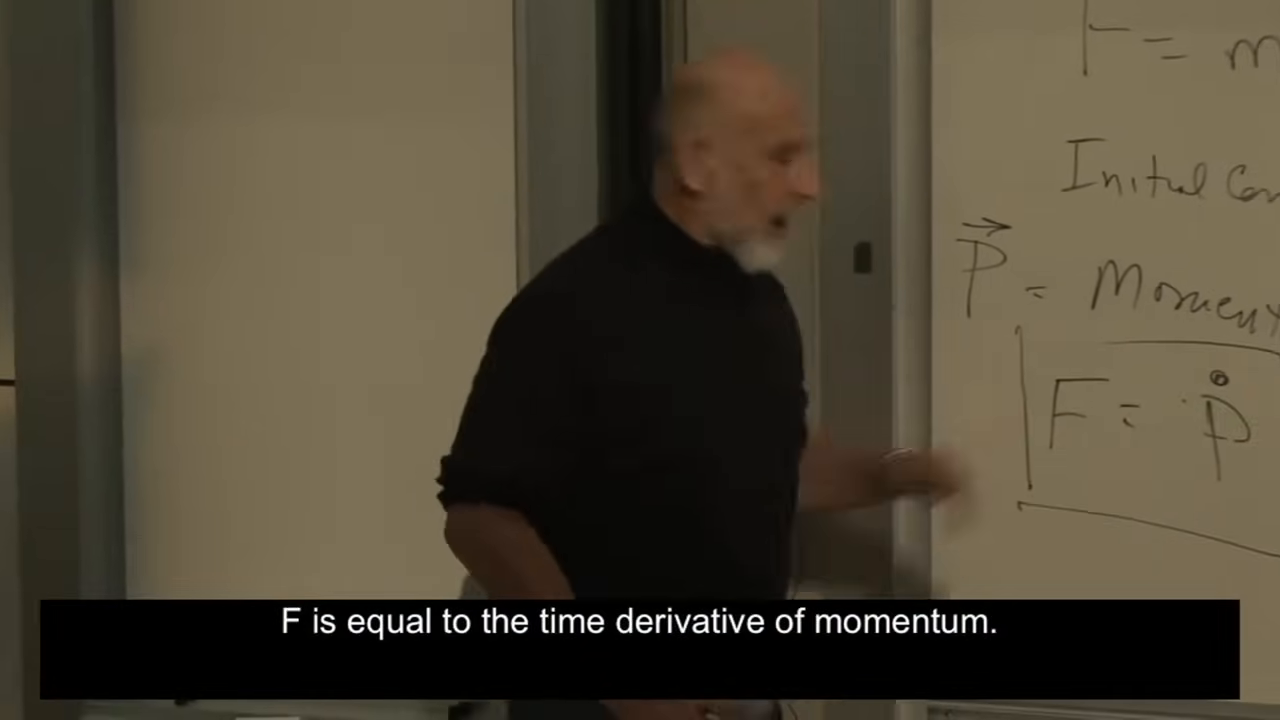
\includegraphics[width=0.82\textwidth]{lecture_02_figure_03.png}
  \caption{Закон Ньютона, записанный через производную импульса по времени.}
  \lectureframe{00:32:35}
\end{figure}

Для одной координаты ньютоновское движение теперь можно записать как два уравнения первого порядка для двух независимых переменных состояния:

\begin{align}
  \dot p&=F(x,t),
  \label{eq:first-order-p}\\
  \dot x&=\frac{p}{m}.
  \label{eq:first-order-x}
\end{align}

Одно уравнение говорит, как сила изменяет импульс; другое — как импульс изменяет положение. Их дискретная форма первого порядка имеет вид

\begin{align}
  p(t+\delta)&=p(t)+\delta F(x(t),t)+O(\delta^2),
  \label{eq:momentum-discrete}\\
  x(t+\delta)&=x(t)+\frac{\delta}{m}p(t)+O(\delta^2).
  \label{eq:position-discrete}
\end{align}

Если заданы \(x(t)\) и \(p(t)\), эти уравнения определяют следующую пару, которая затем служит входом для следующего шага. Траектория строится последовательными обновлениями.

\begin{figure}[htbp]
  \centering
  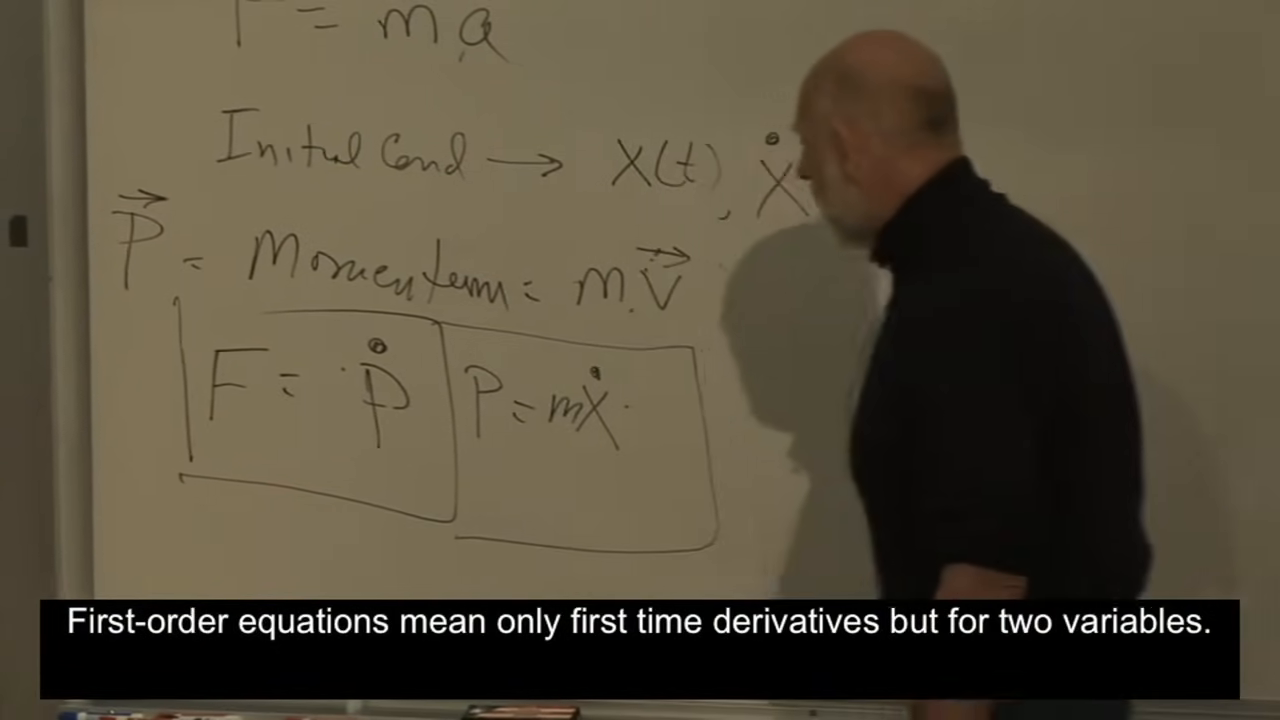
\includegraphics[width=0.84\textwidth]{lecture_02_figure_04.png}
  \caption{Два уравнения первого порядка и соответствующие начальные данные. Положение и импульс вместе задают состояние.}
  \lectureframe{00:35:47}
\end{figure}

Пространство всех пар \((x,p)\) называется \emph{фазовым пространством}. Для одной частицы, движущейся в трёх измерениях, оно имеет шесть координат,

\begin{equation}
  (x,y,z,p_x,p_y,p_z).
  \label{eq:one-particle-phase-space}
\end{equation}

Фазовое пространство — это пространство полных начальных условий. Конфигурационное пространство фиксирует только положения; фазовое пространство фиксирует в точности те данные, которые требуются закону движения.

\begin{classroomqa}
  \audiencequestion{Если сила является функцией положения, а не известной функцией времени, становится ли процедура обновления более сложной?\lecturetimestamp{00:36:27--00:37:07}}
  \lecturerresponse{Уравнения остаются предсказательными. Как только известны \(x\) и \(p\), известна и величина \(F(x)\). Уравнение~\eqref{eq:first-order-p} даёт следующее значение \(p\), уравнение~\eqref{eq:first-order-x} — \(x\), и обновлённую пару можно снова использовать.}
\end{classroomqa}

\section{Ньютоновская пружина}

Вернёмся к пружине, чтобы сравнить два закона в одних и тех же физических условиях. По Ньютону получаем

\begin{equation}
  m\ddot x=-kx.
  \label{eq:newton-spring}
\end{equation}

Временно положим \(m=k=1\), чтобы убрать константы. Тогда

\begin{equation}
  \ddot x=-x.
  \label{eq:normalized-oscillator}
\end{equation}

В отличие от экспоненты, синус либо косинус после двукратного дифференцирования возвращается к себе с противоположным знаком. Общее решение можно записать в виде

\begin{align}
  x(t)&=C\cos(t-t_0),
  \label{eq:oscillator-x}\\
  p(t)=\dot x(t)&=-C\sin(t-t_0).
  \label{eq:oscillator-p}
\end{align}

Эти две константы несут две части начальной информации. Амплитуда \(C\) задаёт максимальное смещение, тогда как \(t_0\) фиксирует фазу, выбранную здесь так, что скорость обращается в нуль при \(t=t_0\). Частица останавливается в концах лишь на мгновение. Затем она проходит обратно через начало координат, где её скорость и импульс максимальны, и продолжает колебаться.

Возводя в квадрат уравнения~\eqref{eq:oscillator-x} и \eqref{eq:oscillator-p}, получаем

\begin{equation}
  x^2+p^2=C^2.
  \label{eq:oscillator-phase-circle}
\end{equation}

Таким образом, точка фазового пространства движется по окружности радиуса \(C\). Разные начальные амплитуды дают разные окружности; изменение \(t_0\) выбирает другую начальную точку на той же окружности. Каждая окружность обходится с одним и тем же периодом \(2\pi\) в этих нормированных единицах, независимо от амплитуды.

\begin{figure}[htbp]
  \centering
  \includegraphics[width=0.84\textwidth]{lecture_02_figure_10.png}
  \caption{Решение осциллятора и его круговая орбита на фазовой плоскости \((x,p)\).}
  \lectureframe{00:43:20}
\end{figure}

\begin{figure}[htbp]
  \centering
  \begin{tikzpicture}[scale=1.05,>=Latex]
    \draw[->] (-2.6,0) -- (2.75,0) node[right] {$x$};
    \draw[->] (0,-2.4) -- (0,2.55) node[above] {$p$};
    \draw[blue!65!black,thick] (0,0) circle (1.85);
    \draw[->,blue!65!black,thick]
      (1.60,0.93) arc[start angle=30,end angle=72,radius=1.85];
    \fill[red!65!black] (1.60,0.93) circle (2pt);
    \draw[dashed] (0,0) -- (1.60,0.93)
      node[midway,below right] {$C$};
    \node[align=left] at (-1.55,1.85)
      {$x=C\cos(t-t_0)$\\$p=-C\sin(t-t_0)$};
  \end{tikzpicture}
  \caption{Орбита в фазовом пространстве сохраняет информацию и о положении, и об импульсе. Её радиус характеризует движение, тогда как угол равномерно растёт со временем.}
  \label{fig:oscillator-phase-space}
\end{figure}

Проекция на горизонтальную ось даёт привычное возвратно-поступательное движение \(x\); проекция на вертикальную ось даёт колебание \(p\). В отличие от аристотелевой пружины, разные окружности никогда не сливаются друг с другом. Знание точки фазового пространства определяет и её будущее, и её прошлое.

Для произвольных \(m\) и \(k\) угловая частота равна

\begin{equation}
  \omega=\sqrt{\frac{k}{m}},
  \qquad
  x(t)=C\cos\bigl(\omega(t-t_0)\bigr),
  \label{eq:general-oscillator-frequency}
\end{equation}

и фазовая орбита становится эллипсом на ненормированной плоскости \((x,p)\). Картина с окружностью соответствует удобной нормировке \(m=k=1\), использованной в лекции.

\begin{classroomqa}
  \audiencequestion{Если бы вторую производную в уравнении осциллятора заменить первой, исчезла бы предсказуемость?\lecturetimestamp{00:45:23--00:46:04}}
  \lecturerresponse{Нет. Уравнение первого порядка всё ещё может предсказывать дальнейшее движение по подходящим начальным данным. Более серьёзный вопрос состоит в том, сохраняет ли порождаемый им поток различия достаточно хорошо, чтобы быть обратимым; соответствующая общая теорема отложена до тех пор, пока не будет введён необходимый аппарат.}
\end{classroomqa}

\section{Обращение времени}

Картина с осциллятором делает обратимость наглядной, но есть и непосредственная проверка на уровне уравнений. Введём обращённую временную координату

\begin{equation}
  T=-t.
  \label{eq:reverse-time}
\end{equation}

Тогда

\begin{equation}
  \frac{d}{dt}=-\frac{d}{dT},
  \qquad
  \frac{d^2}{dt^2}=\frac{d^2}{dT^2}.
  \label{eq:time-derivative-parity}
\end{equation}

Первая производная при обращении времени меняет знак, тогда как вторая — нет. Следовательно, автономное аристотелево уравнение

\begin{equation}
  m\dot x=F(x)
  \label{eq:aristotle-time-reversal}
\end{equation}

не сохраняет своей формы, если прокрутить фильм назад. Затухающая пружина превратилась бы в пружину, которая самопроизвольно уходит от равновесия. Напротив,

\begin{equation}
  m\ddot x=F(x)
  \label{eq:newton-time-reversal}
\end{equation}

не изменяется. При обращении ньютоновского фильма скорость меняет знак, а ускорение остаётся неизменным, так что фильм, прокрученный назад, — это ещё одно допустимое решение.

\begin{figure}[htbp]
  \centering
  \includegraphics[width=0.84\textwidth]{lecture_02_figure_11.png}
  \caption{Сравнение на доске при \(t\mapsto -t\): первые производные меняют знак, тогда как вторые — нет.}
  \lectureframe{00:50:45}
\end{figure}

\begin{classroomqa}
  \audiencequestion{Почему обратимость следует принимать как посылку о физике вообще?\lecturetimestamp{00:46:16--00:48:26}}
  \lecturerresponse{Её проверяют, а не гарантируют определением. Мы рассматриваем успешные законы, выявляем общие экспериментальные особенности и возводим эти особенности в ранг принципов. Более глубокий логический порядок обратный: квантовая теория поля фундаментальнее, а ньютоновская механика возникает через приближения, такие как малые скорости и тяжёлые объекты. Курс должен строиться снизу вверх, начиная с более простых законов, поэтому обратимость вводится сейчас как принцип, область применимости которого будет проверена позже.}
\end{classroomqa}

\begin{classroomqa}
  \audiencequestion{Была ли сама обратимость вопросом, который Ньютон сознательно ставил?\lecturetimestamp{00:48:28--00:49:02}}
  \lecturerresponse{Исторический ответ неопределён. Ньютон, несомненно, понимал инерцию: сила нужна, чтобы изменить состояние движения, а не для поддержания равномерного движения. Оформлял ли он это понимание явно в терминах обратимости — отдельный исторический вопрос.}
\end{classroomqa}

\section{Циклы и сохраняющиеся величины}

Окружности в фазовом пространстве подсказывают следующую идею. Траектория остаётся на одной окружности и никогда не перескакивает на другую. Поэтому каждой окружности можно сопоставить число, которое остаётся постоянным в ходе движения. Для нормированного осциллятора это число равно

\begin{equation}
  C^2=x^2+p^2.
  \label{eq:cycle-label}
\end{equation}

С точностью до множителя одна вторая это энергия осциллятора. Большим окружностям соответствует большая энергия; изменение начальной фазы её не меняет. Мы выведем это утверждение, а не просто прочитаем его с рисунка, но сначала рассмотрим импульс.

Первый закон Ньютона утверждает, что тело, на которое не действует суммарная сила, движется с постоянной скоростью. Он уже содержится во втором законе:

\begin{equation}
  \mathbf F=0
  \quad\Longrightarrow\quad
  \dot{\mathbf p}=0
  \quad\Longrightarrow\quad
  \mathbf v=\text{constant}
  \label{eq:newton-first-from-second}
\end{equation}

при постоянной массе. Третий закон Ньютона вносит действительно новую информацию о взаимодействиях между частицами.

\subsection{Равные, противоположные и центральные силы}

Пусть \(\mathbf F_{ij}\) обозначает силу, действующую на частицу \(i\) со стороны частицы \(j\). Тогда часть третьего закона, утверждающая равенство по величине и противоположность по направлению, имеет вид

\begin{equation}
  \mathbf F_{ij}=-\mathbf F_{ji}.
  \label{eq:newton-third-pair}
\end{equation}

Если бы две силы были направлены в одну и ту же сторону, изолированная пара могла бы самопроизвольно ускоряться. Это была бы машина без рабочего тела, создающая движение только за счет внутренних сил. Такого поведения не наблюдается.

\begin{figure}[htbp]
  \centering
  \includegraphics[width=0.84\textwidth]{lecture_02_figure_12.png}
  \caption{Индексная запись утверждения о равенстве по величине и противоположности сил взаимодействия.}
  \lectureframe{00:59:25}
\end{figure}

Для рассматриваемых здесь сил между точечными частицами обе силы пары, кроме того, направлены вдоль прямой, соединяющей центры частиц. Равные по величине и противоположно направленные силы, не лежащие на одной прямой, могли бы образовать чистый крутящий момент и привести изолированную жесткую пару во вращение. Условие центральной силы исключает эту возможность:

\begin{equation}
  \mathbf F_{ij}\parallel
  (\mathbf r_i-\mathbf r_j).
  \label{eq:central-force-condition}
\end{equation}

Условие равенства и противоположности приводит к сохранению импульса. Условие линии центров связано с законом сохранения момента импульса, который будет изучаться позже.

\begin{figure}[htbp]
  \centering
  \includegraphics[width=0.84\textwidth]{lecture_02_figure_13.png}
  \caption{Центрально-силовая часть третьего закона Ньютона: силы взаимодействия лежат на прямой, соединяющей частицы.}
  \lectureframe{01:01:38}
\end{figure}

\subsection{Полный импульс}

Рассмотрим замкнутую систему из \(N\) частиц. Внешних сил нет; единственные силы — это силы взаимодействия частиц друг с другом. Аддитивность сил и второй закон Ньютона дают для каждой частицы

\begin{equation}
  \dot{\mathbf p}_i
  =m_i\ddot{\mathbf r}_i
  =\sum_{\substack{j=1\\j\ne i}}^N \mathbf F_{ij}.
  \label{eq:many-particle-newton}
\end{equation}

Просуммируем это уравнение по \(i\):

\begin{align}
  \frac{d}{dt}\sum_{i=1}^N\mathbf p_i
  &=\sum_{i=1}^N
    \sum_{\substack{j=1\\j\ne i}}^N\mathbf F_{ij}
  \notag\\
  &=\sum_{i<j}\bigl(\mathbf F_{ij}+\mathbf F_{ji}\bigr)
  =0.
  \label{eq:momentum-pair-cancellation}
\end{align}

Каждое взаимодействие появляется дважды, по одному разу в каждом направлении, и члены пары сокращаются. Введя обозначение

\begin{equation}
  \mathbf P_{\mathrm{tot}}=\sum_{i=1}^N\mathbf p_i,
  \label{eq:total-momentum}
\end{equation}

получаем первый закон сохранения:

\begin{equation}
  \frac{d\mathbf P_{\mathrm{tot}}}{dt}=0.
  \label{eq:momentum-conservation}
\end{equation}

\begin{figure}[htbp]
  \centering
  \includegraphics[width=0.84\textwidth]{lecture_02_figure_14.png}
  \caption{Суммирование уравнений для частиц приводит к сокращению попарных сил, так что производная полного импульса равна нулю.}
  \lectureframe{01:04:38}
\end{figure}

Исторически мы представили сохранение импульса как следствие третьего закона Ньютона. В современной физике сохранение импульса часто рассматривается как более фундаментальное утверждение: если в изолированной двухчастичной системе сохраняется полный импульс, то изменения импульсов ее частиц должны быть равны по величине и противоположны по направлению. Однако для данного изложения полезен именно ньютоновский путь.

\section{Энергия в одном измерении}

Рассмотрим частицу, движущуюся вдоль прямой под действием силы, зависящей только от ее положения:

\begin{equation}
  F=F(x).
  \label{eq:position-force}
\end{equation}

Такая сила называется не зависящей от времени. Это не означает, что сила, действующая на движущуюся частицу, имеет постоянное численное значение. Ее значение меняется по мере изменения \(x(t)\). Это означает, что всякий раз, когда частица находится в одном и том же положении \(x\), на нее действует одна и та же сила, независимо от момента времени.

В одном измерении любую достаточно регулярную функцию силы можно проинтегрировать. Поэтому потенциальную энергию \(V(x)\) определим соотношением

\begin{equation}
  F(x)=-\frac{dV}{dx},
  \label{eq:potential-definition-1d}
\end{equation}

или, что эквивалентно,

\begin{equation}
  V(x)=-\int^x F(u)\,du+V_0.
  \label{eq:potential-integral}
\end{equation}

Аддитивная постоянная \(V_0\) не влияет на силу. Представьте \(V(x)\) как высоту ландшафта над осью \(x\). Частица подталкивается в сторону меньшей высоты, и сила больше там, где наклон круче. В верхней или нижней точке гладкого холма наклон обращается в нуль, так что там сила равна нулю.

\begin{figure}[htbp]
  \centering
  \includegraphics[width=0.84\textwidth]{lecture_02_figure_15.png}
  \caption{Потенциальная энергия как одномерный ландшафт. Сила направлена вниз по склону, а ее величина определяется наклоном.}
  \lectureframe{01:12:57}
\end{figure}

Определим кинетическую, потенциальную и полную энергию соотношениями

\begin{equation}
  T=\frac12m\dot x^2,
  \qquad
  E=T+V(x)
  =\frac12m\dot x^2+V(x).
  \label{eq:energy-1d}
\end{equation}

На данном этапе энергия — это просто название, присвоенное этой предполагаемой сохраняющейся величине. Ее физическую интерпретацию подсказывает картина ландшафта: движение вниз по склону уменьшает \(V\), одновременно увеличивая скорость и, следовательно, \(T\); движение вверх по склону делает обратное. Уравнение Ньютона доказывает, что этот обмен является точным.

Продифференцируем уравнение ~\eqref{eq:energy-1d}. Поскольку \(m\) — постоянная, а \(V\) зависит от времени только через \(x(t)\),

\begin{align}
  \frac{dE}{dt}
  &=m\dot x\ddot x+\frac{dV}{dx}\dot x
  \notag\\
  &=\dot x\left(m\ddot x+\frac{dV}{dx}\right).
  \label{eq:energy-derivative-1d}
\end{align}

Закон Ньютона и определение \(V\) дают

\begin{equation}
  m\ddot x=F=-\frac{dV}{dx}.
  \label{eq:newton-potential-1d}
\end{equation}

Следовательно, выражение в скобках в уравнении ~\eqref{eq:energy-derivative-1d} обращается в нуль:

\begin{equation}
  \frac{dE}{dt}=0.
  \label{eq:energy-conservation-1d}
\end{equation}

\begin{figure}[htbp]
  \centering
  \includegraphics[width=0.84\textwidth]{lecture_02_figure_16.png}
  \caption{Производная энергии в одномерном случае разлагается на множитель скорости и уравнение Ньютона.}
  \lectureframe{01:19:18}
\end{figure}

В одном измерении не потребовалось никакого дополнительного динамического предположения сверх регулярной силы, зависящей от положения, поскольку любая такая сила имеет первообразную.

\section{Несколько измерений и консервативные силы}

Для частицы с координатами \(x_i\) уравнение Ньютона по компонентам имеет вид

\begin{equation}
  F_i(\mathbf x)=m\ddot x_i.
  \label{eq:newton-components}
\end{equation}

Компонента силы \(F_i\) может зависеть от всех координат, а не только от \(x_i\). Мы хотели бы найти одну скалярную функцию \(V(\mathbf x)\) такую, что

\begin{equation}
  F_i(\mathbf x)
  =-\frac{\partial V(\mathbf x)}{\partial x_i},
  \qquad
  \mathbf F=-\boldsymbol\nabla V.
  \label{eq:gradient-force}
\end{equation}

В отличие от одномерного построения, здесь это не происходит автоматически. Три произвольные функции \(F_1,F_2,F_3\), вообще говоря, содержат больше независимой информации, чем производные одной скалярной функции. Эквивалентно, потенциал существует только тогда, когда силовое поле удовлетворяет условиям совместности, например равенству соответствующих смешанных частных производных; в односвязной области это выражается условием \(\boldsymbol\nabla\times\mathbf F=0\). Поэтому уравнение ~\eqref{eq:gradient-force} мы принимаем как физический постулат для рассматриваемого класса сил, а не как математическое тождество.

\begin{figure}[htbp]
  \centering
  \includegraphics[width=0.84\textwidth]{lecture_02_figure_17.png}
  \caption{Многомерный закон силы и контурный эскиз потенциала. Сила направлена поперек линий уровня в сторону убывания \(V\).}
  \lectureframe{01:24:15}
\end{figure}

На контурной карте \(V\) постоянно вдоль каждой линии уровня. Градиент перпендикулярен этим кривым и направлен в сторону наискорейшего возрастания; сила \(-\boldsymbol\nabla V\) направлена в сторону наискорейшего убывания.

\begin{figure}[htbp]
  \centering
  \begin{tikzpicture}[scale=1.0,>=Latex]
    \draw[->] (-3.0,0) -- (3.1,0) node[right] {$x_1$};
    \draw[->] (0,-2.4) -- (0,2.55) node[above] {$x_2$};
    \draw[orange!65!black,thick]
      plot[smooth cycle] coordinates
      {(-0.55,-0.35) (0.15,-0.55) (0.72,-0.10) (0.50,0.53) (-0.25,0.65)};
    \draw[orange!65!black,thick]
      plot[smooth cycle] coordinates
      {(-1.15,-0.75) (0.20,-1.10) (1.35,-0.25) (1.10,0.95) (-0.45,1.25)};
    \draw[orange!65!black,thick]
      plot[smooth cycle] coordinates
      {(-1.85,-1.20) (0.15,-1.70) (2.15,-0.40) (1.70,1.50) (-0.80,1.85)};
    \draw[->,blue!65!black,very thick] (1.62,0.73) -- (0.82,0.20)
      node[midway,above left] {$\mathbf F$};
    \draw[dashed,->,red!65!black,thick] (0.82,0.20) -- (1.62,0.73)
      node[midway,below right] {$\boldsymbol\nabla V$};
    \node[orange!65!black] at (-1.62,1.45) {$V=V_3$};
    \node[orange!65!black] at (-0.92,0.92) {$V=V_2$};
    \node[orange!65!black] at (-0.35,0.30) {$V=V_1$};
  \end{tikzpicture}
  \caption{Линии уровня скалярного потенциала. Градиент нормален к контурам, а консервативная сила направлена в противоположную сторону.}
  \label{fig:potential-contours}
\end{figure}

Когда выполняется уравнение ~\eqref{eq:gradient-force}, определим

\begin{equation}
  E=\frac12m\sum_i\dot x_i^2+V(x_1,\ldots,x_n).
  \label{eq:energy-many-coordinates}
\end{equation}

Кинетический член равен половине массы, умноженной на квадрат длины вектора скорости. Дифференцируя и применяя правило цепочки для функций многих переменных, получаем

\begin{align}
  \frac{dE}{dt}
  &=m\sum_i\dot x_i\ddot x_i
    +\sum_i\frac{\partial V}{\partial x_i}\dot x_i
  \notag\\
  &=\sum_i\dot x_i
    \left(m\ddot x_i+\frac{\partial V}{\partial x_i}\right)
  =0.
  \label{eq:energy-derivative-multidimensional}
\end{align}

Доказательство в точности совпадает с одномерным доказательством, снабжённым индексом, но его предпосылка сильнее: все компоненты силы должны происходить из одного потенциала.

\begin{figure}[htbp]
  \centering
  \includegraphics[width=0.84\textwidth]{lecture_02_figure_18.png}
  \caption{Производная энергии с индексом.  Каждая скобка обращается в нуль в силу соответствующей компоненты уравнения Ньютона.}
  \lectureframe{01:28:30}
\end{figure}

Для \(N\) частиц в трёх измерениях соберём все координаты в один список

\begin{equation}
  \begin{aligned}
    q_a={}&(x_1,y_1,z_1,x_2,y_2,z_2,\ldots,\\[-0.2em]
           &\phantom{(}x_N,y_N,z_N),\\
    &a=1,\ldots,3N.
  \end{aligned}
  \label{eq:flattened-coordinates}
\end{equation}

Имеется \(3N\) координатных компонент, но только \(N\) масс частиц; одна и та же масса повторяется в трёх записях, относящихся к данной частице.  Если

\begin{equation}
  F_a=-\frac{\partial V(q_1,\ldots,q_{3N})}{\partial q_a},
  \label{eq:many-particle-conservative-force}
\end{equation}

тогда

\begin{equation}
  E=\sum_{A=1}^{N}\frac12m_A\lvert\dot{\mathbf r}_A\rvert^2
    +V(\mathbf r_1,\ldots,\mathbf r_N)
  \label{eq:many-particle-energy}
\end{equation}

сохраняется в силу того же вычисления.  Силы, возникающие из потенциала, называются \emph{консервативными} именно потому, что они обеспечивают этот закон сохранения; это прилагательное не имеет политического смысла.

\section{Осциллятор как контур энергии}
\enlargethispage{3\baselineskip}

Для силы пружины \(F=-kx\) уравнение~\eqref{eq:potential-definition-1d} даёт

\begin{equation}
  V(x)=\frac12kx^2+V_0.
  \label{eq:spring-potential}
\end{equation}

При выборе \(V_0=0\) энергия осциллятора равна

\begin{equation}
  E=\frac12m\dot x^2+\frac12kx^2
   =\frac{p^2}{2m}+\frac12kx^2.
  \label{eq:oscillator-energy}
\end{equation}

При \(m=k=1\),

\begin{equation}
  2E=p^2+x^2=C^2.
  \label{eq:oscillator-energy-circle}
\end{equation}

Следовательно, найденные ранее окружности в фазовом пространстве являются контурами постоянной энергии.  Для более общего одномерного потенциала эти контуры не обязаны быть окружностями, но движение всё равно происходит по кривым

\begin{equation}
  \frac{p^2}{2m}+V(x)=E
  \label{eq:general-energy-contour}
\end{equation}

на плоскости \((x,p)\).  Это возвращает нас к идее первой лекции: когда траектории остаются на различных циклах или орбитах, их может обозначать некоторое число, остающееся неизменным на протяжении всего движения.

Теперь у нас есть пространство состояний, ньютоновские уравнения эволюции и первые два закона сохранения.  Следующая формулировка механики начнётся с принципа наименьшего действия и приведёт к лагранжианам, гамильтонианам, моменту импульса и более общей структуре, стоящей за этими примерами.

\begin{classroomqa}
  \audiencequestion{Насколько точно раздаточный материал соответствует тому, что пишется на доске, и где рисунки?\lecturetimestamp{01:37:56--01:38:54}}
  \lecturerresponse{Раздаточный материал должен близко следовать лекции; если в нём отсутствует материал с доски, возможно, был отправлен не тот файл.  Рисунки ещё не были подготовлены; они появятся, шутит он, когда Continuing Studies выплатит следующий чек.}
\end{classroomqa}
\chapter{Стационарное действие и уравнение Эйлера--Лагранжа}

\lectureoverview{Привычное название \emph{принцип наименьшего действия} скрывает существенный момент: физическая траектория делает действие стационарным, но не обязана его минимизировать. Мы выведем это утверждение из обычного равновесия, распространим его с точек на целые функции, получим уравнение Эйлера--Лагранжа, дискретизуя путь, и восстановим уравнения Ньютона. Затем вращающиеся и полярные координаты покажут, почему лагранжева формулировка — это не просто смена обозначений.}

\section{Стационарно, но не обязательно минимально}

Слово \emph{наименьшего} — ненадежная часть традиционного названия. Классическая траектория не всегда делает действие минимумом. Вместо этого она может давать максимум или седло в пространстве возможных траекторий. Правильный принцип состоит в том, что действие \emph{стационарно}: его изменение первого порядка обращается в нуль.

Начнем с более простого вопроса о равновесии. Частица, остающаяся в покое, не имеет ускорения, поэтому равнодействующая сил должна обращаться в нуль. Для силы, получаемой из одномерного потенциала, \begin{equation}
  F(x)=-\frac{dV}{dx},
  \label{eq:force-from-v}
\end{equation} условие равновесия имеет вид \begin{equation}
  \frac{dV}{dx}=0.
  \label{eq:stationary-v-one}
\end{equation}

\begin{figure}[htbp] \centering
  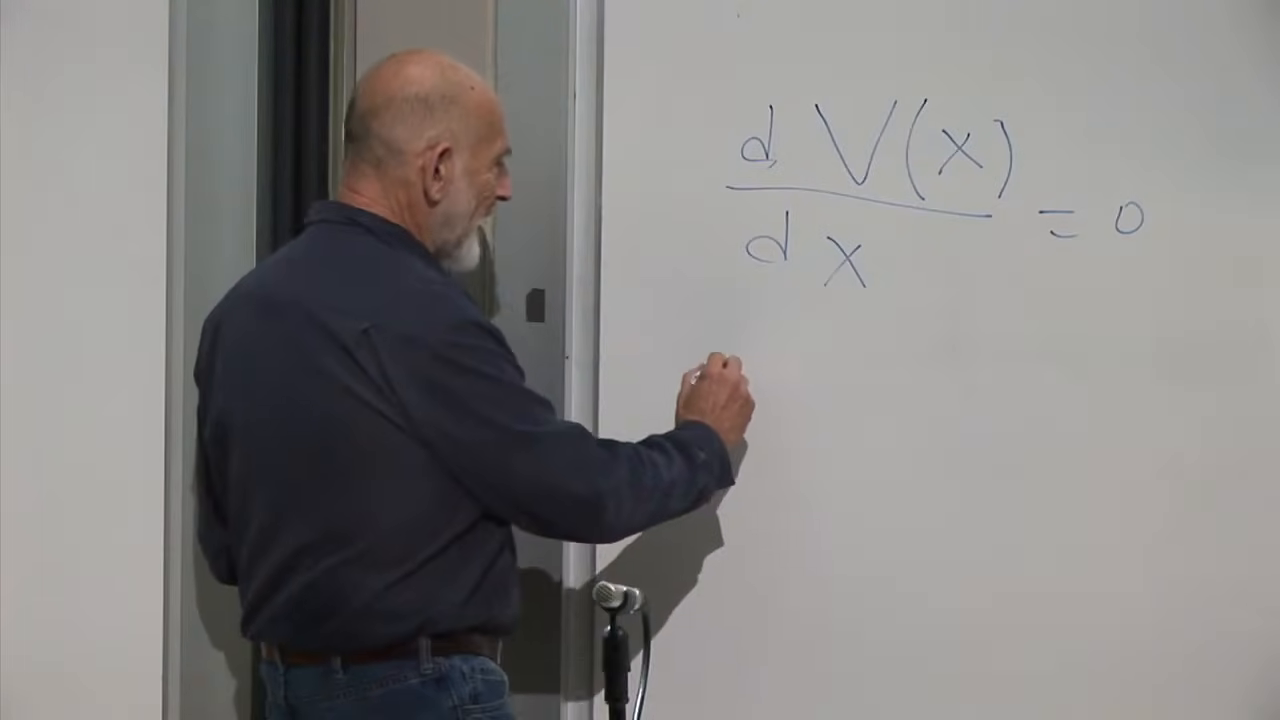
\includegraphics[width=0.74\textwidth]{lecture_03_figure_02.png} \caption{Одномерное условие равновесия: сила обращается в нуль там, где потенциал стационарен.} \lectureframe{00:02:51} \end{figure}

Теперь сместим частицу на малую величину \(\delta x\). В первом порядке \begin{equation}
  \delta V
  =V(x+\delta x)-V(x)
  =\frac{dV}{dx}\,\delta x+O(\delta x^2).
  \label{eq:first-variation-one}
\end{equation} В равновесии линейный член равен нулю при любом знаке \(\delta x\): \begin{equation}
  \delta V=0
  \qquad\hbox{to first order.}
  \label{eq:delta-v-zero-one}
\end{equation} Это не означает, что \(V\) точно не меняется после конечного смещения. Это означает, что главное изменение имеет квадратичный или более высокий порядок. И минимум, и максимум удовлетворяют этому условию.

\begin{figure}[htbp] \centering
  \begin{tikzpicture}[scale=0.95,>=Latex]
    \draw[->] (-0.2,0) -- (3.35,0) node[right] {$x$};
    \draw[->] (0,-0.2) -- (0,2.25) node[above] {$V$};
    \draw[blue!65!black,thick,smooth]
      plot coordinates {(0.2,1.85) (0.75,0.85) (1.55,0.35)
                        (2.35,0.85) (3.0,1.85)};
    \fill[red!65!black] (1.55,0.35) circle (2pt);
    \node at (1.55,-0.34) {minimum};
    \begin{scope}[xshift=4.25cm]
      \draw[->] (-0.2,0) -- (3.35,0) node[right] {$x$};
      \draw[->] (0,-0.2) -- (0,2.25) node[above] {$V$};
      \draw[blue!65!black,thick,smooth]
        plot coordinates {(0.2,0.35) (0.75,1.25) (1.55,1.85)
                          (2.35,1.25) (3.0,0.35)};
      \fill[red!65!black] (1.55,1.85) circle (2pt);
      \node at (1.55,-0.34) {maximum};
    \end{scope}
  \end{tikzpicture} \caption{Стационарность определяет первую производную, но не то, является ли точка минимумом или максимумом.} \label{fig:min-max-stationary} \end{figure}

Для многих координат \(q_i\) первая вариация равна \begin{equation}
  \delta V
  =\sum_i\frac{\partial V}{\partial q_i}\,\delta q_i.
  \label{eq:first-variation-many}
\end{equation} Если она должна обращаться в нуль при любых независимых бесконечно малых смещениях \(\delta q_i\), то каждый коэффициент обращается в нуль: \begin{equation}
  \frac{\partial V}{\partial q_i}=0
  \qquad\hbox{for every }i.
  \label{eq:stationary-v-many}
\end{equation}

Двумерный потенциал лучше представлять себе не как американские горки, а как холмистую местность. Стационарная точка может быть дном долины, вершиной холма или седлом. В седле движение в одном направлении сначала идет вверх, тогда как в другом сначала идет вниз. Поэтому восстанавливающее поведение может быть устойчивым в одном направлении и неустойчивым в другом, хотя все первые производные в самой точке обращаются в нуль.

\begin{figure}[htbp] \centering
  \includegraphics[width=0.76\textwidth]{lecture_03_figure_06.png} \caption{Седло стационарно в первом порядке по любому направлению, хотя соседние смещения вдоль одной оси ведут вверх, а вдоль другой — вниз.} \lectureframe{00:08:20} \end{figure}

В пространстве со многими координатами седловые точки более типичны, чем чистые максимумы или минимумы. Поэтому ключевым словом остается \emph{стационарное}. Условие \begin{equation}
  \delta V=0
  \label{eq:equilibrium-variation}
\end{equation} выражает равновесие, не предрешая поведения второго порядка.

\section{От точек к функциям}

Механика занимается целыми движениями, а не изолированными точками равновесия. Траектория — это функция, такая как \(x(t)\), или совокупность \((x(t),y(t),z(t))\). Математическая задача сделать некоторую величину стационарной, варьируя целую функцию, составляет \emph{вариационное исчисление}. Прежде чем применять его к движению, рассмотрим три более простых примера.

\subsection{Кратчайшие кривые и геодезические}

Зафиксируем две точки на плоскости и представим кривую между ними как \(y(x)\). На коротком участке \begin{equation}
  ds=\sqrt{dx^2+dy^2}
  =dx\sqrt{1+\left(\frac{dy}{dx}\right)^2},
  \label{eq:line-element}
\end{equation} где последняя форма предполагает \(dx>0\). Полная длина есть функцион \begin{equation}
  S[y]=\int_{x_0}^{x_1}
  \sqrt{1+y'(x)^2}\,dx.
  \label{eq:arc-length-functional}
\end{equation} Квадратные скобки подчеркивают, что \(S\) принимает в качестве аргумента целую функцию. Прямая линия выделяется условием \begin{equation}
  \delta S=0
  \label{eq:stationary-length}
\end{equation} при малых изменениях кривой, оставляющих оба конца фиксированными.

\begin{figure}[htbp] \centering
  \includegraphics[width=0.78\textwidth]{lecture_03_figure_07.png} \caption{Пробная кривая между двумя фиксированными концами. Ее длина есть сумма бесконечно малых гипотенуз \(ds\).} \lectureframe{00:13:36} \end{figure}

Тот же вопрос можно задать на искривленной поверхности. Натягивание нити между двумя колышками дает физическую картину кратчайшего пути, ограниченного этой поверхностью. Такая кривая со стационарной длиной — \emph{геодезическая}. На плоскости это прямая линия; на сфере или холмистой поверхности — вообще говоря, нет.

\subsection{Принцип Ферма}

Луч света в среде, где скорость зависит от положения \(c(x,y)\), не обязан следовать по кратчайшему пространственному пути. Время, необходимое для малого участка, равно расстоянию, деленному на локальную скорость, так что \begin{equation}
  T[y]
  =\int_{x_0}^{x_1}
  \frac{\sqrt{1+y'(x)^2}}{c(x,y)}\,dx.
  \label{eq:fermat-functional}
\end{equation} Принцип Ферма требует \begin{equation}
  \delta T=0.
  \label{eq:fermat-stationary}
\end{equation} Если скорость \(c\) постоянна, это сводится к задаче о кратчайшем расстоянии. Однако в среде с переменным показателем преломления быстрейший путь уравновешивает длину пути и локальную скорость распространения.

\begin{figure}[htbp] \centering
  \includegraphics[width=0.80\textwidth]{lecture_03_figure_08.png} \caption{Функционал наименьшего времени для луча в среде, где локальная скорость света зависит от положения.} \lectureframe{00:22:50} \end{figure}

Злободневная шутка отсылает к тогдашнему недавнему заявлению, что в Италии нейтрино двигались необычно быстро. Физический довод сразу возвращается к надежному примеру: обычный свет меняет скорость в веществе в соответствии с показателем преломления.

\subsection{Висящая цепь}

Цепь, закрепленная в двух точках, принимает форму цепной линии. Каждый малый участок вносит вклад в гравитационную потенциальную энергию, так что полная потенциальная энергия сама представляет собой интеграл по цепи. И снова концы фиксированы, неизвестная форма задается функцией, и интеграл должен быть стационарным.

\begin{figure}[htbp] \centering
  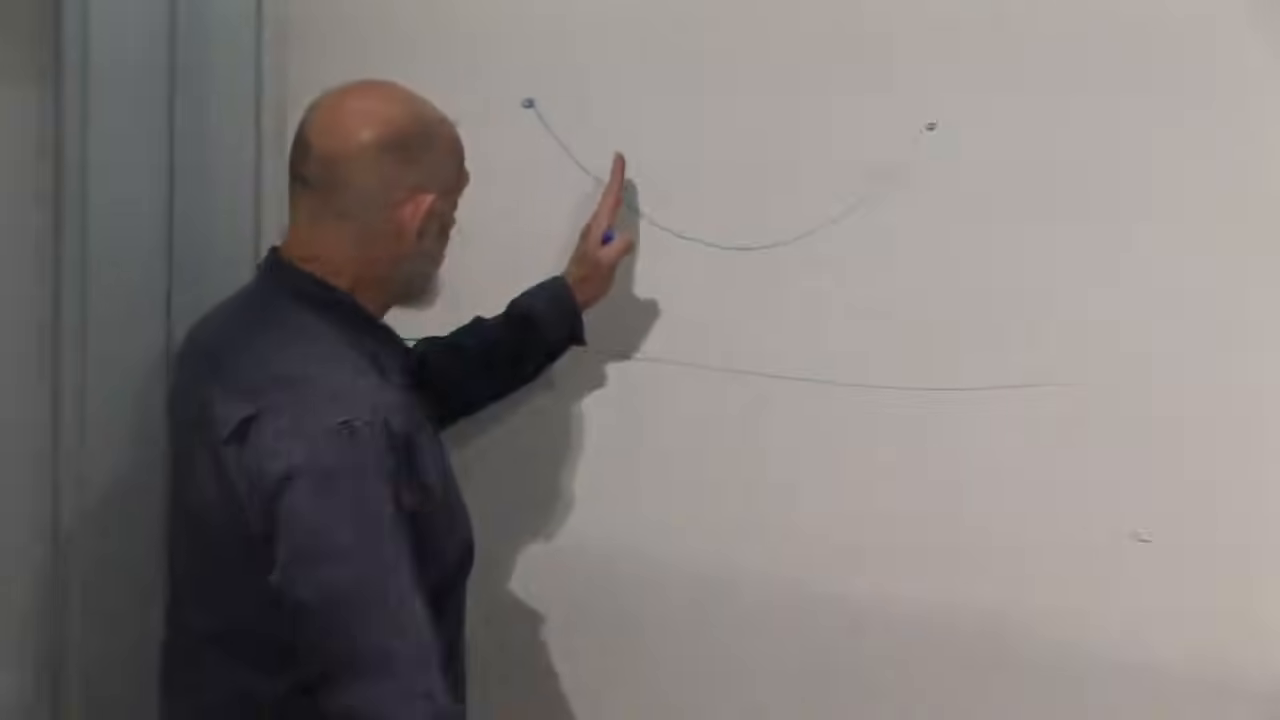
\includegraphics[width=0.76\textwidth]{lecture_03_figure_03.png} \caption{Висящая цепь между фиксированными опорами. Ее стационарная форма определяется полной гравитационной потенциальной энергией.} \lectureframe{00:30:41} \end{figure}

У этих примеров одна и та же структура: два фиксированных конца, функция между ними и интеграл, первая вариация которого обращается в нуль. Свести такое глобальное предписание к дифференциальному уравнению и значит решить вариационную задачу.

\section{Механика как краевая задача}

Траекторию часто изображают с горизонтальной осью времени, потому что \(t\) — независимая переменная. Тем не менее в физике существует устойчивая традиция изображать время направленным вверх. В сторону заметим, что в экспериментах люди располагали картинки от юности к старости в направлениях, связанных с их системами письма: читающие слева направо обычно размещали их слева направо, читающие справа налево — наоборот, а обученные вертикальному письму — по вертикали. Шутка заключает, что физики — это люди, которые настаивают на том, что время течет вверх. Здесь мы будем использовать обычную горизонтальную ось \(t\), потому что тогда \(x(t)\) естественно читается как график.

В формулировке с начальными условиями данные при \(t_0\) имеют вид \begin{equation}
  x(t_0)=x_0,
  \qquad
  \dot x(t_0)=v_0.
  \label{eq:initial-value-data}
\end{equation} Уравнение Ньютона затем определяет дальнейшую траекторию. Вариационная формулировка ставит другую задачу: задать два концевых события, \begin{equation}
  x(t_0)=x_0,
  \qquad
  x(t_1)=x_1,
  \label{eq:boundary-value-data}
\end{equation} и определить физический путь между ними. Начальная скорость больше не задается; она становится частью решения.

\begin{figure}[htbp] \centering
  \includegraphics[width=0.76\textwidth]{lecture_03_figure_09.png} \caption{Механическая траектория \(x(t)\). Можно задать положение и наклон на одном конце либо положения в двух конечных моментах времени.} \lectureframe{00:27:41} \end{figure}

Величина, которую нужно сделать стационарной, — это \emph{действие}, \begin{equation}
  A[x]=\int_{t_0}^{t_1}L(x,\dot x,t)\,dt.
  \label{eq:action-one}
\end{equation} Подынтегральная функция \(L\) — это \emph{функция Лагранжа}. Она может зависеть от положения, скорости и явно от времени. Принцип действия имеет вид \begin{equation}
  \delta A=0
  \label{eq:stationary-action}
\end{equation} для всех малых вариаций пути, при которых \begin{equation}
  \delta x(t_0)=\delta x(t_1)=0.
  \label{eq:fixed-endpoint-variations}
\end{equation} Условие на концах существенно: мы сравниваем соседние пути, соединяющие одни и те же два события.

\section{Дискретный вывод уравнения Эйлера--Лагранжа}

Действие является функционалом бесконечно многих значений траектории. Чтобы сделать его вариацию наглядной, разобьем интервал времени на шаги длины \(\epsilon\), \begin{equation}
  t_n=t_0+n\epsilon,
  \qquad
  x_n=x(t_n),
  \label{eq:discrete-times}
\end{equation} и аппроксимируем скорость на \(n\)-м интервале выражением \begin{equation}
  v_n=\frac{x_{n+1}-x_n}{\epsilon}.
  \label{eq:discrete-velocity}
\end{equation} Интеграл превращается в обычную сумму \begin{equation}
  A_\epsilon
  =\sum_{n=0}^{N-1}
  \epsilon L\left(x_n,\frac{x_{n+1}-x_n}{\epsilon}\right).
  \label{eq:discrete-action}
\end{equation} Мы используем \(n\) как индекс временного слоя, чтобы \(i\) позже можно было использовать для пространственных координат и частиц.

\begin{figure}[htbp] \centering
  \includegraphics[width=0.82\textwidth]{lecture_03_figure_10.png} \caption{Траектория, замененная цепочкой временных слоев. Варьирование одной внутренней ординаты изменяет только два соседних с ней отрезка.} \lectureframe{00:38:30} \end{figure}

Проварьируем одну внутреннюю точку \(x_n\), удерживая все остальные \(x_k\) фиксированными. Только два члена суммы зависят от \(x_n\): \begin{align}
  A_\epsilon\big|_{x_n}
  &=
  \epsilon L\left(x_n,\frac{x_{n+1}-x_n}{\epsilon}\right)
  \notag\\
  &\quad+
  \epsilon L\left(x_{n-1},
                  \frac{x_n-x_{n-1}}{\epsilon}\right).
  \label{eq:two-neighbor-terms}
\end{align} Дифференцируя, получаем \begin{align}
  0=\frac{\partial A_\epsilon}{\partial x_n}
  &=
  \epsilon\frac{\partial L_n}{\partial x_n}
  -\frac{\partial L_n}{\partial v_n}
  +\frac{\partial L_{n-1}}{\partial v_{n-1}}.
  \label{eq:discrete-el-variation}
\end{align} Противоположные знаки имеют простое геометрическое происхождение. Увеличение \(x_n\) увеличивает наклон предшествующего ему интервала и уменьшает наклон следующего за ним интервала.

\begin{figure}[htbp] \centering
  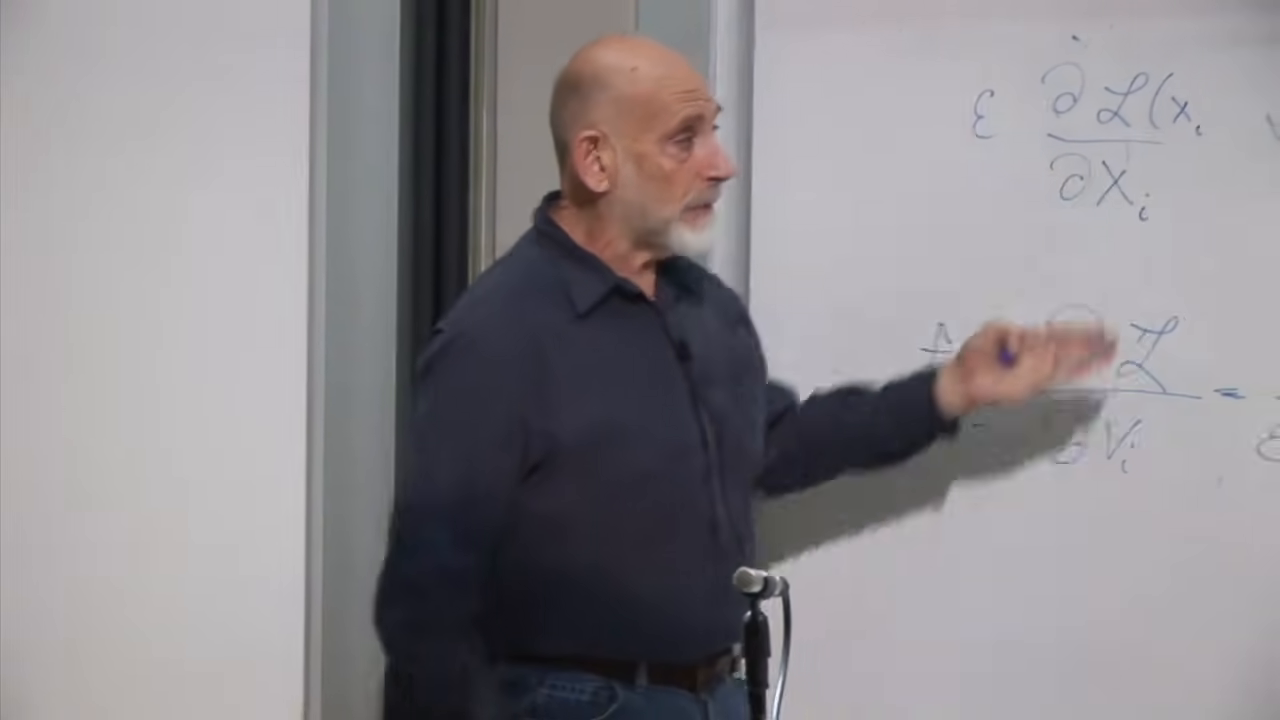
\includegraphics[width=0.74\textwidth]{lecture_03_figure_04.png} \caption{Непосредственная производная по координате и два соседних вклада от производных по скорости в дискретной вариации.} \lectureframe{00:45:26} \end{figure}

Перегруппируем уравнение~\eqref{eq:discrete-el-variation}:
\begin{equation}
  \frac{1}{\epsilon}
  \left(
    \frac{\partial L_n}{\partial v_n}
    -\frac{\partial L_{n-1}}{\partial v_{n-1}}
  \right)
  =
  \frac{\partial L_n}{\partial x_n}.
  \label{eq:discrete-el}
\end{equation}
Левая часть — разностное отношение по соседним точкам. При \(\epsilon\to0\) ломаная превращается в гладкую траекторию, а это отношение становится производной по времени:
\begin{equation}
  \boxed{
  \frac{d}{dt}\left(\frac{\partial L}{\partial\dot x}\right)
  =
  \frac{\partial L}{\partial x}}
  .
  \label{eq:euler-lagrange-one}
\end{equation}
Это уравнение Эйлера--Лагранжа.

\begin{figure}[htbp]
  \centering
  \includegraphics[width=0.78\textwidth]{lecture_03_figure_11.png}
  \caption{Полное уравнение Эйлера--Лагранжа, полученное из условия стационарности на каждом внутреннем временном срезе.}
  \lectureframe{00:49:25}
\end{figure}

Как только задан \(L\), уравнение~\eqref{eq:euler-lagrange-one} работает как вычислительный механизм: продифференцируйте данную функцию, и он выдаст дифференциальное уравнение для траектории.

\begin{classroomqa}
  \audiencequestion{Верно ли результат Эйлера--Лагранжа для любой функции от \(x\) и \(\dot x\)?\lecturetimestamp{00:49:37--00:50:24}}
  \lecturerresponse{Да, при условии той регулярности, которая нужна для существования производных. Пример с длиной дуги после переобозначения имеет в точности ту же форму: его независимая переменная \(x\) играет ту роль, которую здесь играет \(t\), а его неизвестная функция \(y(x)\) — ту роль, которую здесь играет \(x(t)\). Его уравнение Эйлера--Лагранжа имеет решения в виде прямых линий.}
\end{classroomqa}

\section{Уравнения Ньютона из лагранжиана}

Для частицы на прямой в потенциале \(V(x)\) возьмём
\begin{equation}
  L(x,\dot x)=T-V
  =\frac12m\dot x^2-V(x).
  \label{eq:lagrangian-tv-one}
\end{equation}
Знак минус может показаться странным, потому что полная энергия равна \(T+V\). Но лагранжиан — не энергия. Критерий состоит в том, выдаёт ли механизм Эйлера--Лагранжа правильное движение. Устраивать шуточное голосование по поводу знака не будем: ответ нужно проверять, а не выбирать голосованием.

Сначала,
\begin{equation}
  \frac{\partial L}{\partial\dot x}=m\dot x.
  \label{eq:conjugate-momentum-one}
\end{equation}
Это импульс. В более общем случае импульс, сопряжённый любой координате \(q\), определяется как
\begin{equation}
  p_q=\frac{\partial L}{\partial\dot q}.
  \label{eq:conjugate-momentum-general}
\end{equation}
Взяв производную по времени от уравнения~\eqref{eq:conjugate-momentum-one}, получаем \(m\ddot x\), тогда как
\begin{equation}
  \frac{\partial L}{\partial x}
  =-\frac{dV}{dx}.
  \label{eq:lagrangian-position-derivative}
\end{equation}
Следовательно, уравнение Эйлера--Лагранжа имеет вид
\begin{equation}
  m\ddot x=-\frac{dV}{dx}=F(x),
  \label{eq:newton-from-action}
\end{equation}
что и есть второй закон Ньютона.

\begin{figure}[htbp]
  \centering
  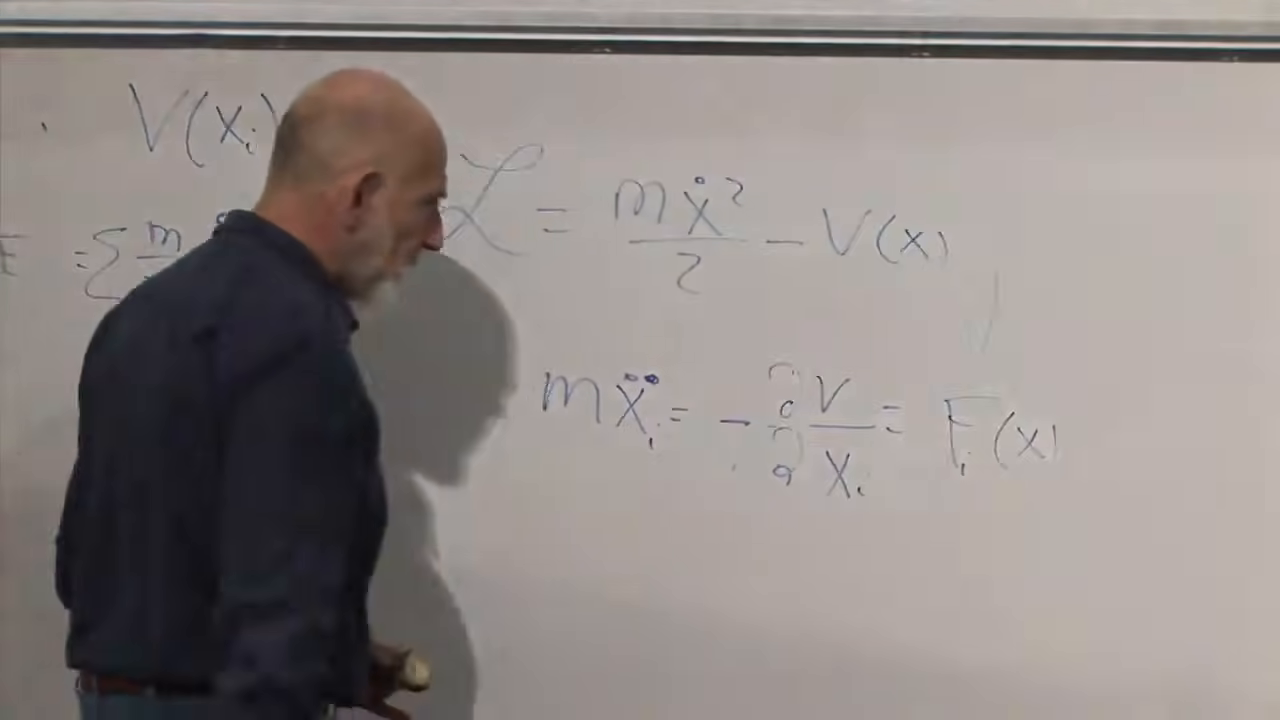
\includegraphics[width=0.80\textwidth]{lecture_03_figure_05.png}
  \caption{Кинетическая энергия, потенциальная энергия, \(L=T-V\) и восстановленная покомпонентная форма уравнения Ньютона на одной доске.}
  \lectureframe{00:57:52}
\end{figure}

Для многих координат \(q_i\),
\begin{equation}
  L(\mathbf q,\dot{\mathbf q})
  =\sum_i\frac12m_i\dot q_i^{\,2}-V(q_1,q_2,\ldots),
  \label{eq:lagrangian-tv-many}
\end{equation}
и для каждой координаты имеется своё уравнение:
\begin{equation}
  \frac{d}{dt}\left(\frac{\partial L}{\partial\dot q_i}\right)
  =\frac{\partial L}{\partial q_i}
  \quad\Longrightarrow\quad
  m_i\ddot q_i=-\frac{\partial V}{\partial q_i}=F_i.
  \label{eq:euler-lagrange-many}
\end{equation}
Траектория по-прежнему остаётся одной кривой, теперь в многомерном конфигурационном пространстве.

\begin{classroomqa}
  \audiencequestion{Неужели мы всего лишь пошли в обратную сторону от закона Ньютона и сконструировали функционал, воспроизводящий ответ?\lecturetimestamp{00:58:07--01:00:04}}
  \lecturerresponse{Это не самая продуктивная точка зрения. Лагранжиан — компактное задание физической системы: одна функция всех координат и скоростей заключает в себе все её уравнения движения. В новых теориях физики обычно предлагают действие и выводят уравнения, а не угадывают каждое уравнение по отдельности.}
\end{classroomqa}

Такая компактная запись — одно из преимуществ. Свобода выбора координат — другое. Утверждение о том, что прямая — кратчайшая линия, не зависит от того, описывается ли плоскость декартовыми, полярными или криволинейными координатами. Точно так же стационарность действия не зависит от выбора координат, хотя формула для \(L\) и получающиеся покомпонентные уравнения меняются.

\section{Свободная частица, наблюдаемая с карусели}

Пусть \((x,y)\) — инерциальные декартовы координаты, а \((X,Y)\) — координаты, равномерно вращающиеся с угловой скоростью \(\omega\). При выбранной здесь ориентации,
\begin{align}
  x&=X\cos\omega t+Y\sin\omega t,
  \notag\\
  y&=-X\sin\omega t+Y\cos\omega t.
  \label{eq:rotating-coordinate-map}
\end{align}
Угол между системами координат равен \(\omega t\).

\begin{figure}[htbp]
  \centering
  \includegraphics[width=0.76\textwidth]{lecture_03_figure_12.png}
  \caption{Инерциальные и равномерно вращающиеся декартовы оси. Одной и той же точке сопоставляются зависящие от времени вращающиеся координаты.}
  \lectureframe{01:06:05}
\end{figure}

Для свободной частицы лагранжиан в инерциальной системе имеет вид
\begin{equation}
  L_{\mathrm{in}}
  =\frac{m}{2}\left(\dot x^2+\dot y^2\right).
  \label{eq:free-inertial-lagrangian}
\end{equation}
Продифференцируем уравнение~\eqref{eq:rotating-coordinate-map} и воспользуемся \(\sin^2\omega t+\cos^2\omega t=1\). Тригонометрические члены объединяются, давая
\begin{align}
  \dot x^2+\dot y^2
  &=
  \dot X^2+\dot Y^2\\
  &\quad+\omega^2(X^2+Y^2)\\
  &\quad+2\omega(Y\dot X-X\dot Y).
  \label{eq:rotating-speed}
\end{align}
Следовательно,
\begin{align}
  L_{\mathrm{rot}}
  &=
  \frac{m}{2}(\dot X^2+\dot Y^2)\\
  &\quad+\frac{m\omega^2}{2}(X^2+Y^2)\\
  &\quad+m\omega(Y\dot X-X\dot Y).
  \label{eq:rotating-lagrangian}
\end{align}

\begin{figure}[htbp]
  \centering
  \includegraphics[width=0.84\textwidth]{lecture_03_figure_13.png}
  \caption{Преобразованный лагранжиан свободной частицы: обычная кинетическая энергия, квадратичный центробежный член и член, линейный по скорости.}
  \lectureframe{01:12:16}
\end{figure}

Квадратичный по координатам член имеет вид \(-V_{\mathrm{fict}}\), где
\begin{equation}
  V_{\mathrm{fict}}
  =-\frac{m\omega^2}{2}(X^2+Y^2).
  \label{eq:centrifugal-potential}
\end{equation}
Он убывает при движении наружу, поэтому создаёт центробежную силу \(m\omega^2(X,Y)\).

Последний член в уравнении~\eqref{eq:rotating-lagrangian} линейный и по координатам, и по скоростям. Применение уравнения Эйлера--Лагранжа даёт
\begin{align}
  m\ddot X&=m\omega^2X-2m\omega\dot Y,
  \notag\\
  m\ddot Y&=m\omega^2Y+2m\omega\dot X.
  \label{eq:rotating-equations}
\end{align}
Члены, пропорциональные \(\omega^2\), являются центробежными; пропорциональные скорости — кориолисовыми. В векторной форме в плоскости вращения,
\begin{equation}
  \mathbf F_{\mathrm{C}}
  =-2m\,\boldsymbol\omega\times\mathbf v_{\mathrm{rot}},
  \label{eq:coriolis-vector}
\end{equation}
причём при выборе противоположной ориентации знаки следует изменить.

\begin{figure}[htbp]
  \centering
  \includegraphics[width=0.84\textwidth]{lecture_03_figure_14.png}
  \caption{Уравнения во вращающейся системе, в которых члены, пропорциональные координатам, дают центробежное ускорение, а перекрёстные скоростные члены — кориолисово ускорение.}
  \lectureframe{01:20:20}
\end{figure}

Суть не в том, что алгебра исчезает. Суть в том, что одно преобразование координат, применённое к одной скалярной функции, порождает и обе связанные уравнения, и обе фиктивные силы.

\begin{classroomqa}
  \audiencequestion{Работает ли этот метод для произвольно криволинейных координат?\lecturetimestamp{01:22:01--01:22:17}}
  \lecturerresponse{Да. Новые координаты могут быть криволинейными и даже явно зависеть от времени, как вращающиеся координаты. Перепишите действие в новых переменных и примените то же правило Эйлера--Лагранжа.}
\end{classroomqa}

\section{Полярные координаты и циклический угол}

Для обычных полярных координат,
\begin{equation}
  x=r\cos\theta,
  \qquad
  y=r\sin\theta.
  \label{eq:polar-map}
\end{equation}
И \(r\), и \(\theta\) могут зависеть от времени. После дифференцирования и сложения квадратов получаем
\begin{equation}
  \dot x^2+\dot y^2
  =\dot r^2+r^2\dot\theta^2.
  \label{eq:polar-speed}
\end{equation}
Для центрального потенциала \(V(r)\),
\begin{equation}
  L
  =\frac{m}{2}\left(\dot r^2+r^2\dot\theta^2\right)-V(r).
  \label{eq:polar-lagrangian}
\end{equation}

\begin{figure}[htbp]
  \centering
  \includegraphics[width=0.80\textwidth]{lecture_03_figure_15.png}
  \caption{Полярная геометрия и разложение кинетической энергии на радиальное и угловое движение.}
  \lectureframe{01:23:30}
\end{figure}

Радиальное уравнение имеет вид
\begin{equation}
  m\ddot r
  =mr\dot\theta^2-\frac{dV}{dr}.
  \label{eq:radial-equation}
\end{equation}
Первый член — направленный наружу центробежный вклад, связанный с собственным угловым движением частицы.

Для угла,
\begin{equation}
  \frac{d}{dt}\left(\frac{\partial L}{\partial\dot\theta}\right)
  =\frac{\partial L}{\partial\theta}=0,
  \label{eq:theta-el}
\end{equation}
поскольку центральный потенциал не имеет явной зависимости от \(\theta\). Следовательно,
\begin{equation}
  \frac{d}{dt}\left(mr^2\dot\theta\right)=0,
  \qquad
  mr^2\dot\theta=\ell,
  \label{eq:angular-momentum}
\end{equation}
где \(\ell\) — сохраняющийся момент импульса.

\begin{figure}[htbp]
  \centering
  \includegraphics[width=0.82\textwidth]{lecture_03_figure_16.png}
  \caption{Угловое уравнение Эйлера--Лагранжа имеет нулевую правую часть, выявляя сохранение \(mr^2\dot\theta\).}
  \lectureframe{01:29:25}
\end{figure}

Угловое уравнение даёт
\begin{equation}
  \dot\theta=\frac{\ell}{mr^2}.
  \label{eq:theta-dot-angular-momentum}
\end{equation}
Подстановка в уравнение~\eqref{eq:radial-equation} оставляет одно уравнение для \(r\):
\begin{equation}
  m\ddot r
  =\frac{\ell^2}{mr^3}-\frac{dV}{dr}.
  \label{eq:effective-radial-equation}
\end{equation}

Координату, отсутствующую в \(L\), традиционно называют \emph{циклической}, даже если она не является углом. Если \(q\) циклическая, то
\begin{equation}
  \frac{\partial L}{\partial q}=0
  \quad\Longrightarrow\quad
  \frac{d}{dt}\left(\frac{\partial L}{\partial\dot q}\right)=0.
  \label{eq:cyclic-conservation}
\end{equation}
Её сопряжённый импульс сохраняется. Это первое указание на общую связь между симметрией и законом сохранения.

\section{Вопросы о смысле, энергии и области применимости}

Следующие вопросы показывают, где заключено более глубокое содержание этого формализма.

\begin{classroomqa}
  \audiencequestion{Есть ли независимое основание прийти к лагранжиану, кроме обнаружения того, что он даёт правильные классические уравнения?\lecturetimestamp{01:33:25--01:35:07}}
  \lecturerresponse{Исторически более чем столетнее развитие классической механики показало, что частицы, волны и электромагнитные поля могут быть представлены в этой форме. На классическом уровне этот накопленный успех является эмпирическим фактом о том, как организованы законы. Более глубокое объяснение приходит из квантовой механики и пока откладывается.}
\end{classroomqa}

\begin{classroomqa}
  \audiencequestion{В лагранжиане во вращающейся системе можно ли отнести линейный по скорости член к обычной кинетической или потенциальной энергии?\lecturetimestamp{01:35:08--01:36:23}}
  \lecturerresponse{Нет. Сохраняющаяся величина, связанная со сдвигом по времени, получается гамильтоновым построением, а не из попытки читать каждый член в \(L\) как кинетическую или потенциальную энергию. Для уравнения~\eqref{eq:rotating-lagrangian} линейный по скорости член сокращается в \(\sum_a\dot q_a\,\partial L/\partial\dot q_a-L\). Гамильтонов подход систематизирует это.}
\end{classroomqa}

Действительно, поскольку \(L_{\mathrm{rot}}\) не зависит явно от времени,
\begin{equation}
  \begin{aligned}
    H_{\mathrm{rot}}
    &=\dot X\frac{\partial L}{\partial\dot X}
     +\dot Y\frac{\partial L}{\partial\dot Y}-L\\
    &=\frac{m}{2}(\dot X^2+\dot Y^2)
     -\frac{m\omega^2}{2}(X^2+Y^2)
  \end{aligned}
  \label{eq:rotating-hamiltonian-preview}
\end{equation}
сохраняется. Это интеграл Якоби во вращающейся системе, а не то же самое численное значение энергии, которое приписывает инерциальный наблюдатель. Зависящие от времени преобразования координат не обязаны сохранять численную форму энергии.

\begin{classroomqa}
  \audiencequestion{Что, если искривлённая траектория вызвана гравитацией?\lecturetimestamp{01:36:30--01:37:10}}
  \lecturerresponse{Для ньютоновской гравитации просто используйте \(V(r)=-GMm/r\) в лагранжиане центральной силы. Искривлённое пространство-время относится к общей теории относительности и здесь не предполагается.}
\end{classroomqa}

\begin{classroomqa}
  \audiencequestion{Не являются ли центробежный потенциал и соответствующая ему энергия всего лишь фиктивными?\lecturetimestamp{01:37:13--01:40:14}}
  \lecturerresponse{Наблюдатель на вращающейся платформе измеряет эффективные силы и может последовательно использовать сохраняющуюся величину во вращающейся системе. Слово \emph{фиктивный} означает, что эти члены возникают из неинерциального описания, а не что их наблюдаемые эффекты воображаемы. Сама энергия не инвариантна при общем зависящем от времени преобразовании координат.}
\end{classroomqa}

\begin{classroomqa}
\audiencequestion{Куда направлена зависящая от скорости сила Кориолиса?\lecturetimestamp{01:40:22--01:42:36}}
\lecturerresponse{Она перпендикулярна скорости во вращающейся системе отсчёта; её величина пропорциональна скорости и угловой скорости системы отсчёта. В плоскости компоненты меняют местами \(\dot X\) и \(\dot Y\) с противоположными знаками, как в уравнении~\eqref{eq:rotating-equations}.}
\end{classroomqa}

\begin{figure}[htbp]
\centering
  \includegraphics[width=0.76\textwidth]{lecture_03_figure_17.png}
\caption{Перекрёстная структура скоростных компонент: сила Кориолиса перпендикулярна скорости во вращающейся системе отсчёта.}
\lectureframe{01:41:40}
\end{figure}

\begin{classroomqa}
\audiencequestion{Должен ли исходный лагранжиан быть записан в инерциальной системе отсчёта?\lecturetimestamp{01:42:37--01:44:00}}
\lecturerresponse{Для обычной свободной частицы ньютоновский закон в инерциальной системе отсчёта даёт простую исходную форму \(m(\dot x^2+\dot y^2)/2\). Когда этот физический закон известен, действие можно преобразовать к любым другим координатам. Не следует независимо предполагать ту же простую кинетическую формулу во вращающейся системе отсчёта.}
\end{classroomqa}

Такой же тип линейного по скорости члена возникает для заряженной частицы в магнитном поле:
\begin{equation}
  L_{\mathrm{em}}
  =\frac12m\mathbf v^2
   +q\mathbf A(\mathbf r,t)\cdot\mathbf v
   -q\phi(\mathbf r,t).
  \label{eq:electromagnetic-lagrangian}
\end{equation}
Для однородного магнитного поля, перпендикулярного плоскости, симметричная калибровка \(\mathbf A=\tfrac12\mathbf B\times\mathbf r\) даёт член, пропорциональный \(X\dot Y-Y\dot X\), с той же алгебраической структурой, что и кориолисов член.

\begin{figure}[htbp]
\centering
  \includegraphics[width=0.82\textwidth]{lecture_03_figure_18.png}
\caption{Линейный по скорости член во вращающейся системе отсчёта, который лежит в основе сравнения с заряженной частицей в однородном магнитном поле.}
\lectureframe{01:44:40}
\end{figure}

\begin{classroomqa}
\audiencequestion{Есть ли, помимо гладкости, ограничения на то, какая функция может служить лагранжианом?\lecturetimestamp{01:44:46--01:45:06}}
\lecturerresponse{Да, но соответствующие ограничения требуют большей структуры, чем пока было введено, и потому отложены. На данном этапе главный урок состоит в том, как предложенный лагранжиан порождает уравнения и законы сохранения.}
\end{classroomqa}

Уравнения во вращающейся системе также допускают круговое движение: точка, покоящаяся в инерциальной системе отсчёта, в системе карусели видна как движущаяся по окружности вокруг начала координат. Магнитная аналогия тогда объясняет, почему заряженная частица может совершать круговое циклотронное движение.

\begin{classroomqa}
\audiencequestion{Останется ли заряженная частица на этой окружности, или излучение приведёт к схлопыванию орбиты?\lecturetimestamp{01:46:11--01:47:21}}
\lecturerresponse{В обсуждаемых уравнениях, описывающих только частицу, излучение не учитывается. Если включить связь с электромагнитным полем и радиационную реакцию, то ускоряющийся классический заряд может излучать. Следовательно, излучение — это дополнительный физический эффект, а не противоречие этой орбите в усечённых уравнениях.}
\end{classroomqa}

\begin{classroomqa}
\audiencequestion{Как ураганы связаны с этим обсуждением?
\lecturetimestamp{01:47:30--01:47:50}}
\lecturerresponse{Их крупномасштабное атмосферное движение происходит на вращающейся Земле, поэтому эффекты Кориолиса важны. Соответствующий вывод относится к метеорологии и здесь не предпринимается.}
\end{classroomqa}

\begin{classroomqa}
\audiencequestion{Ожидается ли, что формализм действия охватывает каждый физический закон, и что означало бы подлинное исключение?\lecturetimestamp{01:47:57--01:49:01}}
\lecturerresponse{Всякую известную замкнутую фундаментальную теорию в рамках обсуждаемой области можно сформулировать через действие: ньютоновские частицы, поля Максвелла, общая теория относительности и Стандартная модель. Кажущиеся контрпримеры, такие как вязкое сопротивление, возникают, когда степени свободы окружающей среды опущены. Если расширить систему, включив жидкость или микроскопическую среду, то фундаментальное описание снова укладывается в этот формализм. Поэтому по-настоящему фундаментальное исключение было бы крупным открытием.}
\end{classroomqa}
\chapter{Симметрия и законы сохранения}

\lectureoverview{Стационарное действие и уравнения Эйлера--Лагранжа составляют одну половину сердца классической механики; гамильтонова формулировка — другую. Здесь мы разовьём первую половину настолько, чтобы выявить глубокую закономерность: каждая непрерывная симметрия лагранжиана порождает сохраняющуюся величину. Мы обнаружим эту закономерность на примере трансляций и вращений, докажем её для общего бесконечно малого преобразования, а затем внимательно рассмотрим, где этот аргумент применим, а где нет.}

\section{Минимум математики, объясняющий физику}

Записи, уже имеющиеся на доске, могут немного напоминать уравнение Шрёдингера, но это не тема сегодняшнего вечера. Тема — симметрия и законы сохранения. Нет честного способа объяснить их связь без уравнений. Сами уравнения элементарны; важно расположить их так, чтобы структура стала видимой. В Scientific American результат можно просто назвать, но здесь нам нужен минимум математики, необходимый, чтобы вывести его так, как это делают физики.

Введём малый параметр \(\epsilon\). Мы сохраняем члены, пропорциональные \(\epsilon\), и отбрасываем \(O(\epsilon^2)\). Это сокращённая запись предельного перехода, а не утверждение, будто у ненулевого действительного числа буквально нулевой квадрат. Для обычной функции \(f(x,y)\),
\begin{equation}
  \delta f
  =\frac{\partial f}{\partial x}\,\delta x
   +\frac{\partial f}{\partial y}\,\delta y
   +O(\epsilon^2),
  \label{eq:first-variation-f}
\end{equation}
где и \(\delta x\), и \(\delta y\) пропорциональны \(\epsilon\). Обозначение \(\delta f\) означает изменение \(f\), а не произведение числа, называемого \(\delta\), на \(f\). Для стационарной точки выполняется
\begin{equation}
  \delta f=0
  \qquad\hbox{to first order.}
  \label{eq:stationary-f}
\end{equation}

Для механической траектории \(q_i(t)\) аналогичной величиной является действие
\begin{equation}
  S[q]=\int_{t_1}^{t_2}L(q,\dot q,t)\,dt.
  \label{eq:action-l4}
\end{equation}
Варьирование траектории при фиксированных концах даёт
\begin{equation}
  \delta S
  =\int_{t_1}^{t_2}dt\,
   \sum_i\left(
     \frac{\partial L}{\partial q_i}\,\delta q_i
     +\frac{\partial L}{\partial\dot q_i}\,\delta\dot q_i
   \right).
  \label{eq:action-variation-l4}
\end{equation}
Эти два члена возникают потому, что изменение траектории изменяет и координаты, и скорости. Интегрирование по частям вместе с условием
\(\delta q_i(t_1)=\delta q_i(t_2)=0\) превращает \(\delta S=0\) в
\begin{equation}
  \frac{d}{dt}\left(\frac{\partial L}{\partial\dot q_i}\right)
  -\frac{\partial L}{\partial q_i}=0.
  \label{eq:el-l4}
\end{equation}

\begin{figure}[htbp]
  \centering
  \includegraphics[width=0.76\textwidth]{lecture_04_figure_05.png}
  \caption{Уравнение Эйлера--Лагранжа, напомненное как отправная точка для симметрии и законов сохранения.}
  \lectureframe{00:09:00}
\end{figure}

Правильное выражение — \emph{стационарное действие}, а не обязательно наименьшее действие. К этому различию мы вернёмся ближе к концу.

\section{Обобщённые координаты и сопряжённый импульс}

Декартовы координаты положения — слишком узкий язык для общей механики. Координатами могут быть положения частиц, углы, коллективные переменные или амплитуды полей, поэтому мы обозначаем их как \(q_i\). Лагранжиан — это сжатое задание динамики. Даже Стандартная модель, если записать её без очень сжатых обозначений, занимает примерно страницу; запись отдельного уравнения движения для каждой компоненты поля заняла бы несравненно больше. Одна функция \(L\) объединяет всё это.

Сопряжённый к \(q_i\) импульс равен
\begin{equation}
  p_i=\frac{\partial L}{\partial\dot q_i}.
  \label{eq:canonical-momentum-l4}
\end{equation}
Вот почему обобщённые координаты традиционно называют \(q\): соответствующие импульсы — это \(p\), так что у нас получаются наши \(p\) и \(q\). В этих обозначениях уравнение~\eqref{eq:el-l4} принимает вид
\begin{equation}
  \dot p_i=\frac{\partial L}{\partial q_i}.
  \label{eq:momentum-el-l4}
\end{equation}

Для привычной одномерной частицы,
\begin{equation}
  L=\frac{m\dot x^2}{2}-V(x),
  \qquad
  \frac{\partial L}{\partial\dot x}=m\dot x,
  \label{eq:particle-momentum-l4}
\end{equation}
так что сопряжённый импульс совпадает с обычным импульсом.

\begin{figure}[htbp]
  \centering
  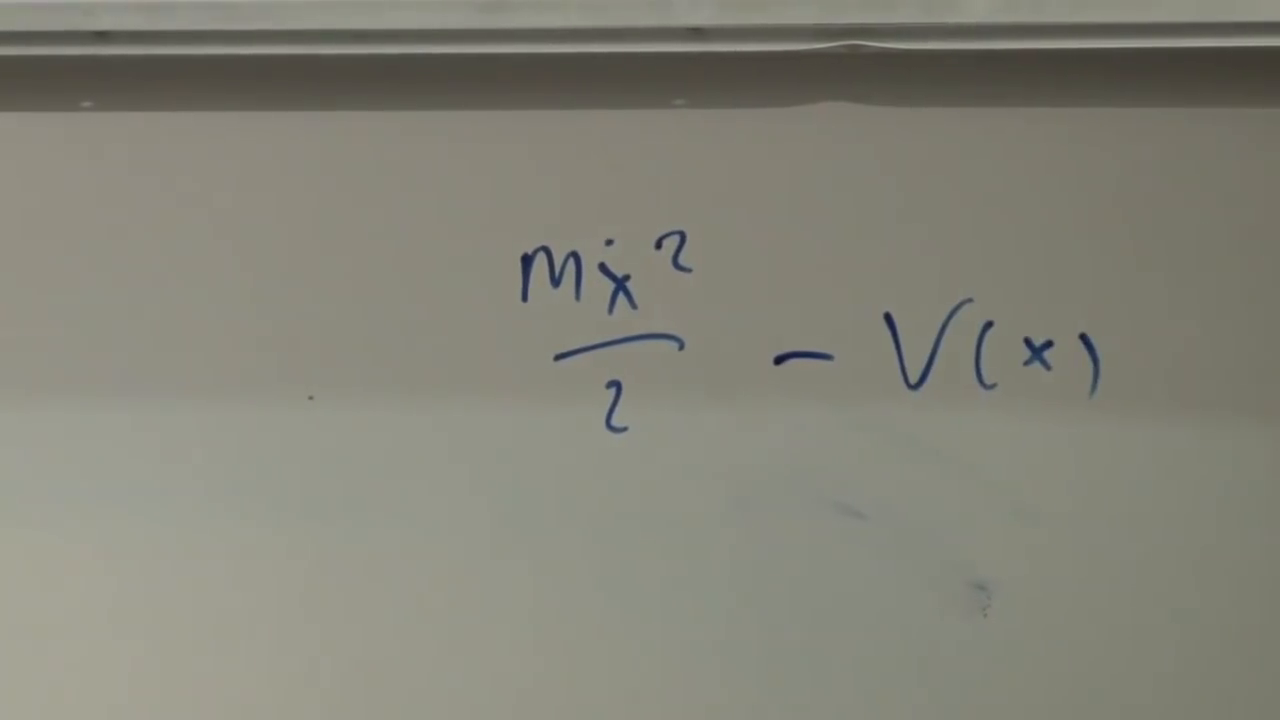
\includegraphics[width=0.72\textwidth]{lecture_04_figure_02.png}
  \caption{Лагранжиан вида «кинетическая энергия минус потенциальная», используемый для отождествления сопряжённого импульса с \(m\dot x\).}
  \lectureframe{00:14:48}
\end{figure}

Если \(q_i\) не входит в \(L\), то \(\dot p_i=0\). Это привычный путь от циклической координаты к закону сохранения. Однако настоящая связь более общая, и полезно сначала обнаружить её на примерах, прежде чем доказывать.

\section{Законы сохранения, обнаруженные до их объяснения}

\subsection{Две координаты и потенциал, зависящий от разности координат}

Положим обе массы равными единице и возьмём
\begin{equation}
  L=\frac{\dot q_1^{\,2}+\dot q_2^{\,2}}{2}-V(q_1-q_2).
  \label{eq:separation-lagrangian}
\end{equation}
Можно представить себе две частицы на прямой. Их взаимодействие зависит только от разности их координат.

\begin{figure}[htbp]
  \centering
  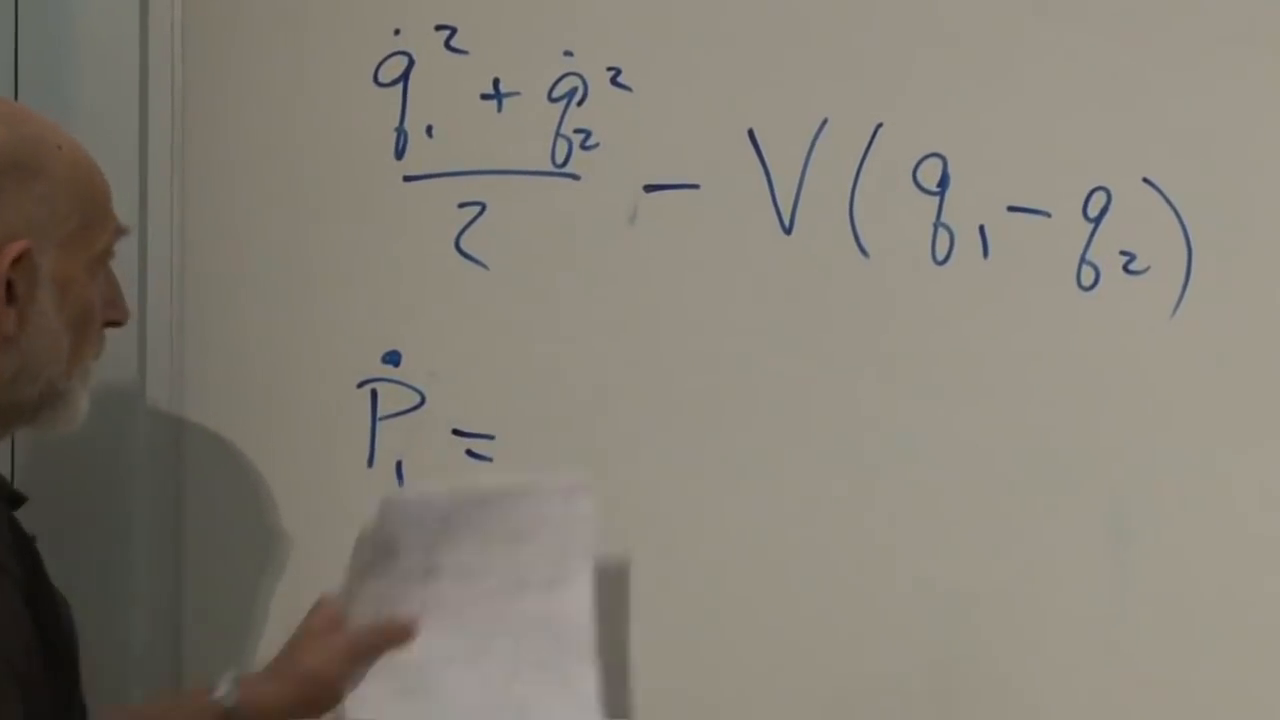
\includegraphics[width=0.78\textwidth]{lecture_04_figure_03.png}
  \caption{Лагранжиан с двумя координатами и начало первого уравнения для импульса.}
  \lectureframe{00:18:56}
\end{figure}

Обозначая через \(V'\) производную по аргументу \(V\),
\begin{align}
  \dot p_1&=-V'(q_1-q_2),
  \notag\\
  \dot p_2&=+V'(q_1-q_2).
  \label{eq:separation-momentum-equations}
\end{align}
Знак во втором уравнении меняется на противоположный, потому что увеличение \(q_2\) уменьшает \(q_1-q_2\).

\begin{classroomqa}
  \audiencequestion{Должно ли первое уравнение для импульса содержать \(V'\), и откуда берётся его знак минус?
  \lecturetimestamp{00:20:52--00:21:35}}
  \lecturerresponse{Уравнение Эйлера--Лагранжа утверждает \(\dot p_1=\partial L/\partial q_1\), а не то, что лагранжиан равен нулю. Поскольку \(L=T-V\), дифференцирование по \(q_1\) даёт \(-V'\). Дифференцирование по \(q_2\) даёт ещё один знак минус из \(q_1-q_2\), поэтому во втором уравнении стоит \(+V'\).}
\end{classroomqa}

\begin{figure}[htbp]
  \centering
  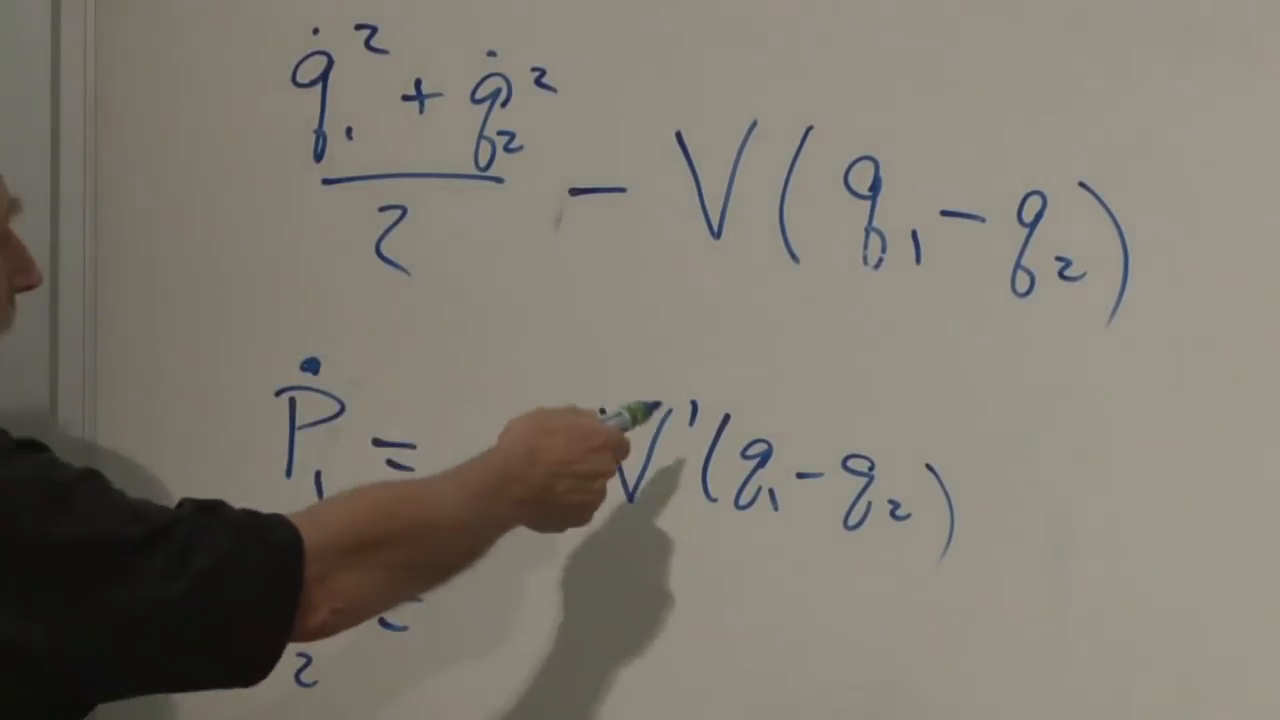
\includegraphics[width=0.78\textwidth]{lecture_04_figure_04.png}
  \caption{Чувствительная к знаку производная в уравнении для \(p_1\); уравнение для \(p_2\) получает противоположный знак.}
  \lectureframe{00:20:41}
\end{figure}

Складывая уравнения~\eqref{eq:separation-momentum-equations}, получаем
\begin{equation}
  \frac{d}{dt}(p_1+p_2)=0.
  \label{eq:total-p-conserved}
\end{equation}
Мы нашли сохраняющуюся величину, но ещё не объяснили, почему она существует.

\subsection{Менее очевидная линейная комбинация}

Теперь пусть
\begin{equation}
  L=\frac{\dot q_1^{\,2}+\dot q_2^{\,2}}{2}
    -V(Aq_1+Bq_2),
  \label{eq:ab-lagrangian}
\end{equation}
где \(A\) и \(B\) — константы. Тогда
\begin{align}
  \dot p_1&=-A\,V'(Aq_1+Bq_2),
  \notag\\
  \dot p_2&=-B\,V'(Aq_1+Bq_2).
  \label{eq:ab-momentum-equations}
\end{align}
Умножая первое уравнение на \(B\), второе на \(A\) и вычитая, исключаем силу:
\begin{equation}
  \frac{d}{dt}(Bp_1-Ap_2)=0.
  \label{eq:ab-conserved}
\end{equation}

\begin{figure}[htbp]
  \centering
  \includegraphics[width=0.78\textwidth]{lecture_04_figure_06.png}
  \caption{Взвешенные уравнения для импульса, в которых силовые члены сокращаются в \(Bp_1-Ap_2\).}
  \lectureframe{00:24:20}
\end{figure}

\begin{classroomqa}
  \audiencequestion{Откуда физически могут возникнуть такие константы, как \(A\) и \(B\)?\lecturetimestamp{00:25:09--00:30:15}}
  \lecturerresponse{Рассмотрим две частицы масс \(m\) и \(M\):
  \[
    L=\frac{m\dot X^2}{2}+\frac{M\dot Y^2}{2}-V(X-Y).
  \]
  Перейдём к \(Q_1=\sqrt m\,X\) и \(Q_2=\sqrt M\,Y\). Кинетический член становится \((\dot Q_1^2+\dot Q_2^2)/2\), тогда как потенциал зависит от \(Q_1/\sqrt m-Q_2/\sqrt M\). Таким образом, неодинаковые массы естественно становятся коэффициентами линейной комбинации. Замена \(Q_2\) на \(-Q_2\) меняет показанный минус на плюс, не изменяя квадратичного кинетического члена.}
\end{classroomqa}

\begin{figure}[htbp]
  \centering
  \includegraphics[width=0.82\textwidth]{lecture_04_figure_07.png}
  \caption{Координаты, взвешенные массами, упрощают кинетическую энергию, перенося массовые множители в потенциал.}
  \lectureframe{00:28:40}
\end{figure}

\begin{classroomqa}
  \audiencequestion{Показывает ли это, что сохраняющаяся величина может существовать без циклической координаты?\lecturetimestamp{00:31:13--00:31:58}}
  \lecturerresponse{В записанных переменных нет \emph{очевидной} циклической координаты. Замена переменных может её выявить, но искать её здесь — не самый полезный подход. Аргумент, основанный на симметрии, прямо укажет сохраняющуюся комбинацию.}
\end{classroomqa}

\section{Что мы понимаем под симметрией}

\subsection{Трансляции}

Начнём со свободной частицы единичной массы,
\begin{equation}
  L=\frac{\dot q^2}{2}.
  \label{eq:free-unit-l4}
\end{equation}
Сдвинем каждую точку её траектории на одну и ту же константу:
\begin{equation}
  q'(t)=q(t)+\epsilon.
  \label{eq:free-translation}
\end{equation}
Поскольку \(\epsilon\) не зависит от времени, \(\dot q'=\dot q\), и потому \(\delta L=0\). Эта инвариантность и есть трансляционная симметрия.

Есть две эквивалентные картины. В пассивной мы сдвигаем начало координат, оставляя объект фиксированным. В активной мы оставляем оси фиксированными и перемещаем объект. Активный язык окажется менее запутывающим: переместим физическую конфигурацию и спросим, замечает ли это \(L\).

Для формулы~\eqref{eq:separation-lagrangian} сдвинем обе координаты:
\begin{equation}
  \delta q_1=\epsilon,
  \qquad
  \delta q_2=\epsilon.
  \label{eq:common-translation}
\end{equation}
Скорости не меняются, и \(q_1-q_2\) тоже.

\begin{figure}[htbp]
  \centering
  \includegraphics[width=0.78\textwidth]{lecture_04_figure_08.png}
  \caption{Общая трансляция оставляет разность двух координат неизменной.}
  \lectureframe{00:35:30}
\end{figure}

Для формулы~\eqref{eq:ab-lagrangian} используем менее очевидное преобразование
\begin{equation}
  \delta q_1=B\epsilon,
  \qquad
  \delta q_2=-A\epsilon.
  \label{eq:ab-transformation}
\end{equation}
Снова скорости не меняются, а
\begin{equation}
  \delta(Aq_1+Bq_2)=AB\epsilon-BA\epsilon=0.
  \label{eq:ab-invariant-argument}
\end{equation}
Следовательно, это преобразование является симметрией.

\begin{figure}[htbp]
  \centering
  \includegraphics[width=0.80\textwidth]{lecture_04_figure_09.png}
  \caption{Асимметричная трансляция, сохраняющая \(Aq_1+Bq_2\).}
  \lectureframe{00:40:20}
\end{figure}

\begin{classroomqa}
  \audiencequestion{Коэффициенты кодируют массы, так что сохраняющаяся величина становится обычным импульсом центра масс?
  \lecturetimestamp{00:42:25--00:42:45}}
  \lecturerresponse{Да. В переменных, взвешенных по массам, симметрия и сохраняющаяся комбинация выглядят несимметрично. При обратном переходе к \(X\) и \(Y\) восстанавливаются обычный одновременный перенос и полный импульс.}
\end{classroomqa}

\subsection{Повороты}

Рассмотрим одну частицу на плоскости,
\begin{equation}
  L=\frac{m}{2}(\dot x^2+\dot y^2)-V(x^2+y^2).
  \label{eq:central-lagrangian-l4}
\end{equation}
Это центральный потенциал. Мы сравниваем две фиксированные системы координат, повернутые друг относительно друга; оси не вращаются со временем. При одном согласованном выборе ориентации,
\begin{align}
  x'&=x\cos\theta+y\sin\theta,
  \notag\\
  y'&=-x\sin\theta+y\cos\theta.
  \label{eq:finite-rotation-l4}
\end{align}

\begin{figure}[htbp]
  \centering
  \includegraphics[width=0.82\textwidth]{lecture_04_figure_10.png}
  \caption{Лагранжиан для центрального потенциала и две фиксированные декартовы системы координат, связанные поворотом.}
  \lectureframe{00:45:40}
\end{figure}

Положим \(\theta=\epsilon\) и сохраним члены первого порядка:
\begin{equation}
  \cos\epsilon=1+O(\epsilon^2),
  \qquad
  \sin\epsilon=\epsilon+O(\epsilon^3).
  \label{eq:small-angle-l4}
\end{equation}
Тогда бесконечно малый поворот имеет вид
\begin{align}
  \delta x&=y\epsilon,
  &\delta y&=-x\epsilon,
  \notag\\
  \delta\dot x&=\dot y\epsilon,
  &\delta\dot y&=-\dot x\epsilon.
  \label{eq:infinitesimal-rotation-l4}
\end{align}

\begin{figure}[htbp]
  \centering
  \includegraphics[width=0.82\textwidth]{lecture_04_figure_11.png}
  \caption{Бесконечно малый поворот координат и скоростей.}
  \lectureframe{00:49:50}
\end{figure}

В отличие от переноса, величина изменения \(x\) зависит от \(y\), а величина изменения \(y\) зависит от \(x\). Тем не менее,
\begin{align}
  \delta(x^2+y^2)
  &=2x\,\delta x+2y\,\delta y=0,
  \notag\\
  \delta(\dot x^2+\dot y^2)
  &=2\dot x\,\delta\dot x+2\dot y\,\delta\dot y=0.
  \label{eq:rotation-invariants-l4}
\end{align}
И потенциальный, и кинетический члены инвариантны.

\begin{figure}[htbp]
  \centering
  \includegraphics[width=0.76\textwidth]{lecture_04_figure_12.png}
  \caption{Сокращение в первом порядке, показывающее, что квадрат радиуса инвариантен относительно поворотов.}
  \lectureframe{00:53:20}
\end{figure}

\section{Общая теорема о сохранении}

Примеры с переносом и поворотом имеют одну общую форму. Пусть непрерывное бесконечно малое преобразование имеет вид
\begin{equation}
  \delta q_i=\epsilon f_i(q),
  \qquad
  \delta\dot q_i=\frac{d}{dt}\delta q_i,
  \label{eq:general-infinitesimal-symmetry}
\end{equation}
где \(\epsilon\) не зависит от времени, а \(f_i\) может зависеть от всех координат.

\begin{figure}[htbp]
  \centering
  \includegraphics[width=0.78\textwidth]{lecture_04_figure_13.png}
  \caption{Общее поле бесконечно малых смещений
  \(\delta q_i=\epsilon f_i(q)\).}
  \lectureframe{00:56:00}
\end{figure}

Вариация лагранжиана в первом порядке равна
\begin{equation}
  \delta L
  =\sum_i\left(
    \frac{\partial L}{\partial q_i}\delta q_i
    +\frac{\partial L}{\partial\dot q_i}\delta\dot q_i
  \right).
  \label{eq:delta-l-general}
\end{equation}

\begin{figure}[htbp]
  \centering
  \includegraphics[width=0.84\textwidth]{lecture_04_figure_14.png}
  \caption{Два вклада в \(\delta L\): вариация координат и вариация скоростей.}
  \lectureframe{01:02:30}
\end{figure}

Теперь ограничимся физической траекторией, так что выполняются уравнения Эйлера--Лагранжа. Используя
\begin{equation}
  \frac{\partial L}{\partial\dot q_i}=p_i,
  \qquad
  \frac{\partial L}{\partial q_i}=\dot p_i,
  \label{eq:el-substitution-l4}
\end{equation}
получаем
\begin{align}
  \delta L
  &=\sum_i\left(\dot p_i\,\delta q_i
                +p_i\,\delta\dot q_i\right)
  \notag\\
  &=\frac{d}{dt}\sum_i p_i\delta q_i
  =\epsilon\frac{d}{dt}\sum_i p_i f_i(q).
  \label{eq:noether-derivation-l4}
\end{align}
Ключевой шаг здесь — всего лишь правило произведения.

Если преобразование является симметрией, то \(\delta L=0\). Поскольку \(\epsilon\) — произвольный постоянный множитель,
\begin{equation}
  \boxed{
  \frac{d\mathcal Q}{dt}=0,
  \qquad
  \mathcal Q=\sum_i p_i f_i(q)}
  .
  \label{eq:noether-charge-l4}
\end{equation}
Это — ядро теоремы Нётер в классической механике для точных, не зависящих от времени точечных симметрий.

\begin{figure}[htbp]
  \centering
  \includegraphics[width=0.84\textwidth]{lecture_04_figure_15.png}
  \caption{Шаг с правилом произведения, который превращает инвариантность \(L\) в сохраняющуюся величину.}
  \lectureframe{01:05:00}
\end{figure}

\begin{classroomqa}
  \audiencequestion{В \(f_i(q)\) должен ли \(q\) иметь ещё один индекс?
  \lecturetimestamp{01:06:57--01:07:31}}
  \lecturerresponse{Обозначение \(q\) без индекса означает весь набор
  \((q_1,q_2,\ldots)\). Каждая компонента \(f_i\) может зависеть от всех этих
  координат. Например, для поворота \(f_x=y\) и \(f_y=-x\).}
\end{classroomqa}

Теперь эти примеры перестают быть случайными. Для одновременного переноса
\(f_1=f_2=1\), поэтому
\begin{equation}
  \mathcal Q=p_1+p_2.
  \label{eq:noether-common-p}
\end{equation}
Для несимметричного переноса \(f_1=B\), \(f_2=-A\), поэтому
\begin{equation}
  \mathcal Q=Bp_1-Ap_2.
  \label{eq:noether-ab-p}
\end{equation}
Для поворота \(f_x=y\) и \(f_y=-x\):
\begin{equation}
  \mathcal Q=p_xy-p_yx.
  \label{eq:rotation-charge-sign}
\end{equation}
С точностью до знака, зависящего от ориентации, это угловой момент,
\begin{equation}
  J=xp_y-yp_x.
  \label{eq:angular-momentum-l4}
\end{equation}

\begin{figure}[htbp]
  \centering
  \includegraphics[width=0.82\textwidth]{lecture_04_figure_16.png}
  \caption{Нётеровский заряд для поворотов, равный с точностью до ориентации плоскому угловому моменту.}
  \lectureframe{01:11:00}
\end{figure}

Для многих взаимодействующих частиц следует поворачивать все частицы вместе. Тогда из инвариантности следует сохранение суммы их угловых моментов, а не углового момента каждой частицы по отдельности.

\section{Вопросы о предпосылках теоремы}

\begin{classroomqa}
  \audiencequestion{Вносила бы вращающаяся система осей явную зависимость от времени в \(\delta L\)?\lecturetimestamp{01:12:57--01:13:57}}
  \lecturerresponse{Да. Только что приведённое доказательство предполагает не зависящий от времени параметр симметрии: фиксированный перенос или фиксированный поворот. Преобразование, параметр которого зависит от времени, даёт дополнительные члены и требует более общего рассмотрения.}
\end{classroomqa}

\begin{classroomqa}
  \audiencequestion{Является ли заглавное \(Q\) в формуле на доске самим преобразованием?\lecturetimestamp{01:14:02--01:15:58}}
  \lecturerresponse{Нет. Это обозначение, к сожалению, конфликтует с координатами \(q_i\). Преобразование имеет вид
  \(\delta q_i=\epsilon f_i(q)\); соответствующая сохраняющаяся величина равна
  \(\mathcal Q=\sum_i p_i f_i\). Коэффициент \(f_i\) показывает, как изменяется \(i\)-я координата при данной симметрии.}
\end{classroomqa}

Сохранение энергии тоже порождается симметрией, но другой: переносом по времени, то есть независимостью от того, где расположен нуль времени. Этот случай и гамильтонова формулировка будут рассмотрены позже.

\begin{classroomqa}
  \audiencequestion{Можно ли поглотить реальное движение в изменяющуюся систему координат, так что механика станет не чем иным, как координатными преобразованиями?\lecturetimestamp{01:17:43--01:20:01}}
  \lecturerresponse{Можно выбрать координаты, следующие за некоторым конкретным движением, но тогда преобразование зависит от начального состояния и от траектории. Используемое здесь преобразование симметрии фиксируется независимо от того, какому решению следует система. Само движение естественнее представлять в объединённом пространстве координат и импульсов.}
\end{classroomqa}

\section{Гармонический осциллятор в фазовом пространстве}

Полагая массу и жёсткость пружины равными единице,
\begin{equation}
  L=\frac{\dot q^2}{2}-\frac{q^2}{2}.
  \label{eq:oscillator-l4}
\end{equation}
Из определения сопряжённого импульса и уравнения движения получаем
\begin{equation}
  p=\dot q,
  \qquad
  \dot p=-q,
  \label{eq:oscillator-first-order-l4}
\end{equation}
или
\begin{equation}
  \dot q=p,
  \qquad
  \dot p=-q.
  \label{eq:oscillator-phase-flow}
\end{equation}
Эти уравнения описывают равномерное круговое движение на плоскости \(q\)-\(p\). Осциллятор в обычном пространстве, движущийся туда и обратно, есть проекция этой окружности на ось \(q\): скорость максимальна при \(q=0\) и обращается в нуль в точках поворота.

\begin{figure}[htbp]
  \centering
  \includegraphics[width=0.82\textwidth]{lecture_04_figure_17.png}
  \caption{Уравнения гармонического осциллятора и соответствующая им круговая орбита в пространстве \(q\)-\(p\).}
  \lectureframe{01:25:30}
\end{figure}

\begin{classroomqa}
  \audiencequestion{Обходится ли окружность в фазовом пространстве по часовой стрелке?
  \lecturetimestamp{01:25:47--01:27:15}}
  \lecturerresponse{Если \(p\) откладывается по горизонтали, а \(q\) по вертикали, то да. При максимальном положительном \(q\) имеем \(\dot p=-q<0\), так что движение направлено вниз. Если изменить расположение осей, визуальное направление изменится на противоположное; поэтому эту договорённость легко запомнить неверно.}
\end{classroomqa}

Пара уравнений в ~\eqref{eq:oscillator-phase-flow} уже напоминает уравнения Гамильтона, но получена целиком в рамках лагранжевой механики.

\section{Непрерывные и дискретные симметрии}

\begin{classroomqa}
  \audiencequestion{Должна ли симметрия выражаться бесконечно малым декартовым преобразованием?\lecturetimestamp{01:27:48--01:30:31}}
  \lecturerresponse{Декартовы координаты лишь удобны; существенное требование для этого доказательства — непрерывность. У некоторых симметрий нет бесконечно малой версии. Для чётного потенциала отражение переводит
  \(q\mapsto -q\) и \(\dot q\mapsto-\dot q\), оставляя \(L\) неизменным, но
  отражение нельзя составить из сколь угодно малых отражений.
  Поэтому этот классический вывод не даёт соответствующей сохраняющейся величины.}
\end{classroomqa}

\begin{figure}[htbp]
  \centering
  \includegraphics[width=0.82\textwidth]{lecture_04_figure_18.png}
  \caption{Чётный потенциал инвариантен относительно дискретного отражения
  \(q\mapsto -q\).}
  \lectureframe{01:29:30}
\end{figure}

\begin{classroomqa}
  \audiencequestion{Если сохраняющаяся величина \(\mathcal Q\) ненулевая, показывает ли это, что преобразование не было симметрией?
  \lecturetimestamp{01:30:40--01:31:30}}
  \lecturerresponse{Нет. Сохраняющаяся величина может иметь любое постоянное значение. Существенная проверка — это \(\dot{\mathcal Q}\). Если величина, полученная из некоторого предполагаемого преобразования, не сохраняется, то при предпосылках данного доказательства это предполагаемое преобразование не было симметрией.}
\end{classroomqa}

\begin{classroomqa}
  \audiencequestion{Отражение всё же оставляет лагранжиан неизменным, так почему из него не получается закон сохранения?\lecturetimestamp{01:31:34--01:32:27}}
  \lecturerresponse{Одна лишь инвариантность видна сразу, но в выводе использовались смещение первого порядка и правило произведения. Отражение переносит одну сторону конфигурационного пространства на другую одним дискретным шагом. При отсутствии бесконечно малого генератора \(f_i\) формуле \(\mathcal Q=\sum_i p_i f_i\) просто нечего использовать.}
\end{classroomqa}

\begin{classroomqa}
  \audiencequestion{Как называется свойство, при котором преобразование строится из сколь угодно малых преобразований?\lecturetimestamp{01:32:36--01:33:23}}
  \lecturerresponse{Это \emph{непрерывная симметрия}. Перенос и поворот непрерывны; отражение — \emph{дискретная симметрия}.}
\end{classroomqa}

\begin{classroomqa}
  \audiencequestion{Если из многих бесконечно малых шагов получается конечное преобразование, не могут ли отброшенные ошибки \(O(\epsilon^2)\) накопиться?
  \lecturetimestamp{01:33:23--01:36:10}}
  \lecturerresponse{Инвариантность относительно бесконечно малого преобразования должна выполняться в каждой точке, достигаемой в ходе преобразования, а не только в начальной. Разбейте конечный интервал параметра на \(N\) шагов размера \(\epsilon\): накопленное смещение первого порядка равно \(N\epsilon\), тогда как локальный остаток \(O(\epsilon^2)\) накапливается как \(N\epsilon^2=(N\epsilon)\epsilon\to0\). Именно эта структура перехода от локального к конечному и формализуется непрерывными группами преобразований.}
\end{classroomqa}

\begin{classroomqa}
  \audiencequestion{Реализуются ли дискретные симметрии физически в классических системах?\lecturetimestamp{01:36:32--01:37:25}}
  \lecturerresponse{Разумеется. У самого гармонического осциллятора потенциал чётный, \(V(q)\propto q^2\), поэтому он инвариантен относительно \(q\mapsto -q\). Таких примеров много; суть лишь в том, что эта дискретная инвариантность не даёт нового классического нётеровского заряда.}
\end{classroomqa}

\begin{classroomqa}
  \audiencequestion{Но если и непрерывные, и дискретные преобразования оставляют \(L\) неизменным, разве это не одно и то же условие?
  \lecturetimestamp{01:37:37--01:39:18}}
  \lecturerresponse{Это одно и то же утверждение об инвариантности относительно конечного преобразования, но не одна и та же математическая предпосылка для данного доказательства. Для доказательства нужна вариация первого порядка. Для отражения «первый порядок» не имеет смысла, так что цепочку уравнений, ведущую к заряду, нельзя даже начать.}
\end{classroomqa}

\begin{classroomqa}
  \audiencequestion{Как это исторически связано с теоремой Нётер?
  \lecturetimestamp{01:39:26--01:40:42}}
  \lecturerresponse{Это ограниченная часть гораздо более общей теоремы Эмми Нётер. Отдельные связи между симметриями и сохраняющимися величинами были известны и раньше, но в начале XX века Нётер поместила их в единую и поразительно общую схему. Её математической значимости не соответствовало справедливое отношение к ней в академической среде.}
\end{classroomqa}

\begin{classroomqa}
  \audiencequestion{Является ли классическая механика по-прежнему предметом активных исследований?
  \lecturetimestamp{01:40:47--01:42:37}}
  \lecturerresponse{Да. Использованная здесь элементарная теорема стара, но нелинейная динамика, интегрируемые системы, хаос, механика жидкостей и геометрическая механика остаются богатыми областями исследований. Принцип симметрии также простирается далеко за пределы классической механики частиц.}
\end{classroomqa}

\section{Почему важен принцип действия}

\begin{classroomqa}
  \audiencequestion{Есть ли интуитивная причина, по которой симметрия должна влечь закон сохранения?\lecturetimestamp{01:42:49--01:47:57}}
  \lecturerresponse{Не из одной лишь симметрии. Рассмотрим вязкое сопротивление,
  \[
    m\ddot x=-c\dot x.
  \]
  Это уравнение инвариантно относительно \(x\mapsto x+\epsilon\), однако при
  \(p=m\dot x\),
  \[
    \dot p=-\frac{c}{m}p,
    \qquad
    p(t)=p(0)e^{-ct/m},
  \]
  так что импульс убывает. Это эффективное уравнение для подсистемы, а не фундаментальный закон, вытекающий из принципа стационарности действия для одного лишь \(x\). Если включить молекулы жидкости и остальную часть замкнутой системы, полный импульс сохраняется. Симметрия и сохранение связываются друг с другом через лагранжев принцип действия, а не через одно только наличие дифференциального уравнения.}
\end{classroomqa}

\begin{figure}[htbp]
  \centering
  \includegraphics[width=0.65\textwidth]{lecture_04_figure_19.png}
  \caption{Инвариантное относительно переносов вязкое сопротивление, при котором импульс частицы в редуцированном описании тем не менее убывает.}
  \lectureframe{01:44:30}
\end{figure}

\begin{classroomqa}
  \audiencequestion{Можно ли количественно определить, в каких случаях физическая траектория не является минимумом действия?\lecturetimestamp{01:48:08--01:51:38}}
  \lecturerresponse{Подлинный минимум — исключение; действие в пространстве траекторий, как правило, имеет седловой характер. Для единичного осциллятора,
  \[
    S[q]=\frac12\int(\dot q^2-q^2)\,dt.
  \]
  Узкая, быстро меняющаяся деформация увеличивает положительный вклад \(\dot q^2\). Широкая деформация, которая в течение долгого времени остаётся слегка смещённой, может сделать преобладающим отрицательный вклад \(-q^2\) и уменьшить действие. Следовательно, у одной и той же стационарной траектории есть направления, в которых действие возрастает, и направления, в которых оно убывает. Квантовая механика в подходе интеграла по траекториям даёт более глубокое объяснение стационарности, но этот аргумент пока откладывается.}
\end{classroomqa}

\begin{figure}[htbp]
  \centering
  \includegraphics[width=0.80\textwidth]{lecture_04_figure_20.png}
  \caption{Широкая соседняя траектория осциллятора иллюстрирует, почему стационарность действия обычно соответствует седлу, а не минимуму.}
  \lectureframe{01:50:20}
\end{figure}

\begin{classroomqa}
  \audiencequestion{Существует ли взаимно-однозначное соответствие между непрерывными симметриями и законами сохранения?\lecturetimestamp{01:51:44--01:52:43}}
  \lecturerresponse{В рамках вариационной постановки и после отождествления эквивалентных или тривиальных случаев это, по существу, верная картина. Каждой непрерывной симметрии соответствует заряд, а сохраняющиеся величины, как правило, можно, в свою очередь, связать с симметриями. Точные формулировки содержат технические оговорки, поэтому этим общим утверждением не следует пользоваться небрежно.}
\end{classroomqa}

\begin{classroomqa}
  \audiencequestion{Должен ли каждый лагранжиан обладать нетривиальной симметрией?
  \lecturetimestamp{01:52:43--01:53:23}}
  \lecturerresponse{Нет. Примеры были выбраны так, чтобы у них были симметрии. Типичный лагранжиан вовсе не обязан быть инвариантным относительно какого бы то ни было рассматриваемого пространственного преобразования.}
\end{classroomqa}

\begin{classroomqa}
  \audiencequestion{Следует ли в конечном счёте понимать симметрию как активное преобразование или как пассивное изменение координат?
  \lecturetimestamp{01:53:25--01:55:08}}
  \lecturerresponse{Обе формулировки можно сделать эквивалентными, но здесь чище активная. Переместите всю физическую систему и спросите, меняется ли лагранжиан. В пассивной формулировке нужно вместо этого говорить, что при перемещении системы отсчёта \emph{форма} лагранжиана не меняется.}
\end{classroomqa}

\begin{classroomqa}
  \audiencequestion{Что дальше?\lecturetimestamp{01:55:10--01:55:35}}
  \lecturerresponse{Сохранение энергии, его происхождение из симметрии относительно сдвигов по времени, а затем гамильтонов формализм.}
\end{classroomqa}
\chapter{Энергия и гамильтониан}

\lectureoverview{Сначала мы уточним смысл активной симметрии и напомним, как трансляции и вращения порождают импульс и момент импульса. Недостающий закон сохранения — это закон сохранения энергии. Соответствующая ему симметрия есть трансляция по времени, а сохраняющаяся величина — гамильтониан \(H=\sum_i p_i\dot q_i-L\). Вывод также точно показывает, как явная зависимость от времени переносит энергию между выбранной подсистемой и её окружением.}

\section{Вопросы перед формальным выводом}

Мы подходим к абсолютному минимуму классической механики, необходимому для последующих тем, хотя в механике ещё очень многое стоит изучить. Перед началом основного вывода возникли два вопроса.

\begin{classroomqa}\audiencequestion{Какие книги полезны после этого вводного курса? \lecturetimestamp{00:00:36--00:02:13}}\lecturerresponse{Общепризнанным продвинутым справочником является \emph{Классическая механика} Герберта Голдстейна. Книга Корнелиуса Ланцоша о вариационных принципах механики — ещё один подходящий источник. Список литературы для курса полезнее, чем делать вид, будто один преподаватель может обозреть все доступные тексты.}\end{classroomqa}

Второй вопрос относится к одному моменту в истории ещё не разрешённого тогда измерения. В 2011 эксперимент OPERA сообщил о кажущемся раннем прибытии нейтрино, посланных из CERN в Gran Sasso. Сообщённое расхождение было меньше по длительности, чем протонный импульс, использованный для рождения нейтрино, поэтому анализ времён опирался на сравнение профилей импульсов, а не на пометку одного нейтрино при испускании и распознавание той же частицы при детектировании.

\begin{classroomqa}\audiencequestion{Был ли уже разрешён кажущийся результат о нейтрино, движущихся быстрее света? \lecturetimestamp{00:02:30--00:09:03}}\lecturerresponse{Тогда нельзя было обоснованно делать никакого вывода. Форма импульса пучка, нагрев мишени и синхронизация — всё это требовало технической проверки. В одном спекулятивном предложении рассматривалось движение спутника GPS: в системе отсчёта спутника источник и детектор движутся, пока распространяются сигналы синхронизации, что даёт поправки порядка десятков наносекунд. Эта оценка была интересна как упражнение на оценку порядка величины, но её не предлагали как правдоподобный диагноз эксперимента. Обычное лоренцево сокращение при соответствующей скорости было слишком мало, чтобы дать сообщённый эффект. Правильной реакцией было дождаться экспериментального анализа.}\end{classroomqa}

\begin{figure}[htbp]\centering
  \includegraphics[width=0.78\textwidth]{lecture_05_figure_07.png}\caption{Схема временного анализа в системе отсчёта спутника, обсуждавшаяся в историческом вопросе об измерении нейтрино.}\lectureframe{00:06:30}\end{figure}

Это обсуждение временного анализа не нужно для дальнейшего изложения механики. Тем не менее оно полезно как напоминание о том, что правдоподобная оценка порядка величины — не то же самое, что установленное экспериментальное объяснение.

\section{Активная симметрия и выбор системы}

Вернёмся к пункту, который в предыдущем обсуждении остался слишком расплывчатым: что именно является симметрией? Рассмотрим частицу на прямой и предписание \begin{equation}
  x\longrightarrow x+1.
  \label{eq:l5-shift-one}
\end{equation} Его можно понимать двумя способами. \emph{Пассивное} преобразование переобозначает точки прямой. Точка, которая раньше называлась \(x=0\), теперь может называться \(x'=1\), но частица не сдвинулась. \emph{Активное} преобразование сохраняет метки фиксированными и перемещает саму частицу из \(x\) в \(x+1\). Только вторая операция меняет её положение относительно внешнего потенциала.

\begin{figure}[htbp]\centering
  \includegraphics[width=0.82\textwidth]{lecture_05_figure_08.png}\caption{Правило \(x\mapsto x+1\), фиксированная координатная прямая и внешний потенциал отличают активное перемещение от пассивного переобозначения.}\lectureframe{00:11:20}\end{figure}

\begin{classroomqa}\audiencequestion{Если при перемещении частицы меняется её потенциальная энергия, исключается ли из системы источник этого потенциала? \lecturetimestamp{00:12:19--00:14:18}}\lecturerresponse{Именно. Если назвать систему ``частица в потенциале'', то мы разделяем мир на частицу и массивное окружение, например Землю, которое создаёт \(V(x)\). Земля, конечно, тоже испытывает отдачу, но в этом приближении её огромная масса делает эту отдачу пренебрежимо малой. Перемещение частицы относительно фиксированной Земли может изменить \(V\); совместная трансляция частицы и Земли — нет.}\end{classroomqa}

\begin{classroomqa}\audiencequestion{В предыдущем примере с вращением изменялись ли и скорости, а не только положения? \lecturetimestamp{00:14:26--00:15:29}}\lecturerresponse{Да. Жёсткое активное вращение действует на всю историю движения, а не только на одно мгновенное положение. Поворачиваются и положения, и векторы скорости. Напротив, постоянная трансляция, применяемая во все моменты времени, меняет \(x\), но оставляет \(\dot x\) неизменным.}\end{classroomqa}

Различие между системой и окружением ещё дважды появится: когда зависящая от времени установка обменивается энергией с подсистемой и когда макроскопическое трение скрывает энергию в ненаблюдаемом микроскопическом движении.

\section{Бесконечно малые перемещения в конфигурационном пространстве}

Конфигурация произвольной механической системы есть точка в пространстве обобщённых координат \(q_i\). Активное бесконечно малое преобразование переводит каждую возможную конфигурацию в близкую к ней. Мы пишем \begin{equation}
  \delta q_i=\epsilon f_i(q),
  \label{eq:l5-general-transformation}
\end{equation} где функции \(f_i\) задают одно фиксированное поле смещений в конфигурационном пространстве. Они могут зависеть от всех координат, и некоторые из них могут обращаться в нуль. Общий множитель \(\epsilon\) мал; он отделяет величину шага от формы преобразования.

\begin{figure}[htbp]\centering
  \includegraphics[width=0.75\textwidth]{lecture_05_figure_09.png}\caption{Вектор смещения, сопоставленный каждой точке конфигурационного пространства.}\lectureframe{00:16:50}\end{figure}

\begin{figure}[htbp]\centering
  \includegraphics[width=0.80\textwidth]{lecture_05_figure_10.png}\caption{Зависящее от координат бесконечно малое преобразование \(\delta q_i=\epsilon f_i(q)\).}\lectureframe{00:18:00}\end{figure}

Само это правило не содержит явной зависимости от времени. Поэтому его действие на скорости имеет вид \begin{equation}
  \delta\dot q_i=\frac{d}{dt}(\delta q_i)
  =\epsilon\sum_j\frac{\partial f_i}{\partial q_j}\dot q_j.
  \label{eq:l5-velocity-variation}
\end{equation} Для трансляции \(f_x=1\), поэтому \(\delta\dot x=0\). Для вращения \(f_i\) зависит от положения, и скорость изменяется.

\begin{classroomqa}\audiencequestion{Является ли последний малый множитель в \(\delta q_i=\epsilon f_i(q)\) одной и той же константой во всех точках? \lecturetimestamp{00:19:58--00:20:51}}\lecturerresponse{Да. Одна и та же константа \(\epsilon\) служит служебным параметром, который делает все изменения координат величинами первого порядка по одной и той же малой величине. Пространственная зависимость содержится в функциях \(f_i(q)\), а не в \(\epsilon\), и сами они не обязаны быть малыми.}\end{classroomqa}

\section{Что делает преобразование симметрией?}

Активное преобразование, вообще говоря, изменяет потенциальную энергию. Оно может также изменять кинетическую энергию. В криволинейных координатах кинетический член имеет вид \begin{equation}
  T=\frac12\sum_{i,j}g_{ij}(q)\dot q_i\dot q_j,
  \label{eq:l5-kinetic-metric}
\end{equation} так что перемещение в конфигурационном пространстве может изменить его коэффициенты. Простейший пример — хорошо знакомый член \(r^2\dot\theta^2\) в полярных координатах.

Здесь преобразование является симметрией, если \emph{весь} лагранжиан не меняется в первом порядке, \begin{equation}
  \delta L=O(\epsilon^2),
  \label{eq:l5-symmetry-condition}
\end{equation} и это должно выполняться в каждой точке конфигурационного пространства, а не только в той конфигурации, которую занимает какое-то одно конкретное решение.

Например, при \(x\mapsto x+\epsilon\) \begin{equation}
  \delta V=\frac{\partial V}{\partial x}\epsilon.
  \label{eq:l5-potential-variation}
\end{equation} Если это обращается в нуль при любом возможном \(x\), то \(\partial V/\partial x=0\): потенциал не зависит от \(x\). Если потенциал не меняется при трансляциях по всем пространственным направлениям, то он постоянен.

\begin{figure}[htbp]\centering
  \includegraphics[width=0.80\textwidth]{lecture_05_figure_11.png}\caption{Трансляция по \(x\), проверяемая на потенциале \(V(y)\), не зависящем от \(x\).}\lectureframe{00:23:40}\end{figure}

Для гладкого однопараметрического семейства отсутствие изменения первого порядка в каждой точке позволяет сложить бесконечно малые шаги в конечное симметричное преобразование.

\begin{classroomqa}\audiencequestion{Должны ли кинетическая и потенциальная энергии оставаться инвариантными по отдельности? \lecturetimestamp{00:24:44--00:25:33}}\lecturerresponse{Нет. Инвариантным должен быть только полный лагранжиан. Некоторые лагранжианы содержат смешанные координатно--скоростные члены и не допускают полезного разложения на \(T\) и \(V\), так что отдельная инвариантность может вообще не быть осмысленным вопросом.}\end{classroomqa}

\begin{classroomqa}\audiencequestion{Означает ли ``отсутствие изменения'' ровно отсутствие изменения или лишь изменение, достаточно малое, чтобы им пренебречь? \lecturetimestamp{00:25:34--00:28:59}}\lecturerresponse{Для бесконечно малого преобразования это означает отсутствие члена, пропорционального \(\epsilon\). Члены порядка \(\epsilon^2\) в локальном вычислении отбрасываются. Поскольку условие первого порядка выполняется всюду вдоль однопараметрической орбиты, повторение локального шага даёт инвариантность конечного преобразования.}\end{classroomqa}

\section{Восстановление импульса и момента импульса}

Для рассматриваемых здесь точных, не зависящих от времени точечных симметрий ранее доказанный результат имеет вид \begin{equation}
  Q=\sum_i p_i f_i(q),
  \qquad
  p_i=\frac{\partial L}{\partial\dot q_i},
  \qquad
  \dot Q=0.
  \label{eq:l5-noether-charge}
\end{equation} Множитель \(\epsilon\) не входит в \(Q\); он измеряет только то, насколько далеко мы продвигаемся вдоль орбиты симметрии.

\begin{figure}[htbp]\centering
  \includegraphics[width=0.82\textwidth]{lecture_05_figure_12.png}\caption{Общее бесконечно малое смещение и соответствующий ему сохраняющийся нётеровский заряд.}\lectureframe{00:30:00}\end{figure}

Для переноса вдоль \(x\), \(f_x=1\), а \(Q=p_x\).  Полная инвариантность относительно переносов дает сохранение всех трех компонент импульса.  Для многих взаимодействующих частиц симметрия переносит все частицы вместе, так что
\begin{equation}
  \mathbf P=\sum_a\mathbf p_a
  \label{eq:l5-total-momentum}
\end{equation}
сохраняется, когда взаимодействия зависят только от относительных положений.  Перемещение одной частицы относительно остальных не является этой симметрией.

\begin{figure}[htbp]
  \centering
  \includegraphics[width=0.80\textwidth]{lecture_05_figure_13.png}
  \caption{Общий перенос приводит к сохранению полного импульса по компонентам.}
  \lectureframe{00:32:50}
\end{figure}

Для бесконечно малого поворота в плоскости \(x\)-\(y\) выберем ориентацию
\begin{equation}
  \delta x=-y\epsilon,
  \qquad
  \delta y=x\epsilon.
  \label{eq:l5-planar-rotation}
\end{equation}
Он сохраняет радиус, поскольку
\begin{equation}
  \delta(x^2+y^2)
  =2x\delta x+2y\delta y=0.
  \label{eq:l5-radius-invariance}
\end{equation}

\begin{figure}[htbp]
  \centering
  \includegraphics[width=0.76\textwidth]{lecture_05_figure_14.png}
  \caption{Геометрия и координатная формула бесконечно малого поворота в плоскости.}
  \lectureframe{00:35:05}
\end{figure}

Дифференцируя уравнение ~\eqref{eq:l5-planar-rotation}, получаем, что скорости тоже поворачиваются.  Поэтому \(\dot x^2+\dot y^2\) инвариантно, а центральный потенциал
\(V(\sqrt{x^2+y^2})\) оставляет полный лагранжиан неизменным.  Заряд равен
\begin{equation}
  Q=-yp_x+xp_y=(\mathbf r\times\mathbf p)_z.
  \label{eq:l5-angular-charge}
\end{equation}

\begin{figure}[htbp]
  \centering
  \includegraphics[width=0.76\textwidth]{lecture_05_figure_15.png}
  \caption{Нётеровский заряд вращений, \(z\)-компонента момента импульса.}
  \lectureframe{00:38:50}
\end{figure}

Вращения в других координатных плоскостях дают остальные компоненты.  Для многих частиц сохраняющийся вектор равен
\begin{equation}
  \mathbf J=\sum_a\mathbf r_a\times\mathbf p_a.
  \label{eq:l5-total-angular-momentum}
\end{equation}
Основной пример — планета в центральном потенциале звезды: инвариантность относительно всех вращений влечет сохранение всех компонент момента импульса.

\begin{classroomqa}
  \audiencequestion{Что происходит в остром изломе, где производная с одной стороны отличается от производной с другой?
  \lecturetimestamp{00:42:25--00:44:21}}
  \lecturerresponse{Это правомерная оговорка.  Настоящее рассуждение предполагает дифференцируемые функции с однозначно определенными производными.  Неустойчивое равновесие, например тело, уравновешенное в гладком максимуме, само по себе не является проблемой: производная там существует и обращается в нуль.  Буквальный излом требует модифицированного рассмотрения.}
\end{classroomqa}

\begin{classroomqa}
  \audiencequestion{Если параметр преобразования не зависит от времени, почему при повороте меняются скорости?
  \lecturetimestamp{00:44:23--00:45:23}}
  \lecturerresponse{Параметр постоянен, но поле смещений зависит от координат.  Общее правило таково:
  \(\delta\dot q_i=d(\delta q_i)/dt\).  Для переноса \(\delta x\) постоянно, тогда как для поворота \(\delta x=-y\epsilon\) и поэтому
  \(\delta\dot x=-\dot y\epsilon\).}
\end{classroomqa}

\section{За пределами элементарной формы «кинетическая минус потенциальная»}

В декартовых координатах для обычных нерелятивистских частиц без магнитных полей \(L=T-V\).  Более общие координаты приводят к квадратичной форме из уравнения ~\eqref{eq:l5-kinetic-metric}.  Магнитное поле вносит член, линейный по скорости, схематически \(\mathbf A(q)\cdot\dot{\mathbf q}\), который смешивает координаты и скорости.  В таком случае лучше рассматривать \(L(q,\dot q,t)\) как единую функцию, чем пытаться втиснуть каждый член в привычные рамки кинетической и потенциальной энергии.

\begin{figure}[htbp]
  \centering
  \includegraphics[width=0.80\textwidth]{lecture_05_figure_16.png}
  \caption{Общий квадратичный кинетический член, зависящий от координат, рядом с потенциалом, зависящим только от координат.}
  \lectureframe{00:47:20}
\end{figure}

\begin{classroomqa}
  \audiencequestion{Почему лагранжиан может не раскладываться аккуратно на кинетическую и потенциальную энергии, и определяется ли он тогда по-прежнему как \(T-V\)?
  \lecturetimestamp{00:45:26--00:48:13}}
  \lecturerresponse{Препятствие может возникать из-за криволинейных координат или из-за подлинных зависящих от скорости взаимодействий, таких как магнетизм.  Только когда лагранжиан состоит из квадратичной формы по скоростям минус функции только от координат, мы называем эти части \(T\) и \(V\).  В противном случае лагранжиан остается вполне корректной функцией \(q\) и \(\dot q\), но такое разбиение не приносит пользы.  Корректное общее определение энергии будет получено из гамильтониана.}
\end{classroomqa}

\begin{classroomqa}
  \audiencequestion{Был ли пример с висячей цепью с первой встречи применением принципа наименьшего действия?
  \lecturetimestamp{00:48:15--00:49:45}}
  \lecturerresponse{Это была задача о равновесии, определяемая принципом наименьшей энергии, а не история, выбираемая стационарным действием.  Для статического решения обычной системы \(T-V\), \(\dot p_i=0\), и уравнение Эйлера--Лагранжа сводится к \(\partial V/\partial q_i=0\), условию стационарной точки потенциала.}
\end{classroomqa}

Импульс и момент импульса теперь связаны с пространственными симметриями.  Явно недостающая величина — энергия.

\section{Инвариантность относительно переносов по времени}

Представьте эксперимент, который начинается в \(t_0\), заканчивается в \(t_1\) и дает некоторый результат.  Повторите ту же подготовку позже, начав в \(t_0+\Delta t\) и закончив в \(t_1+\Delta t\).  Если результат не меняется, система инвариантна относительно активного переноса по времени.

\begin{figure}[htbp]
  \centering
  \includegraphics[width=0.82\textwidth]{lecture_05_figure_17.png}
  \caption{Эксперимент и его сдвинутая по времени копия в истории в конфигурационном пространстве.}
  \lectureframe{00:52:45}
\end{figure}

Заряженная частица между пластинами конденсатора иллюстрирует нарушение этой симметрии.  При фиксированном заряде пластин один и тот же эксперимент можно выполнять в любое время.  Если внешний генератор непрерывно заряжает пластины, частица испытывает разное электрическое поле в зависимости от того, когда ее отпускают.  Тогда она является подсистемой с явным внешним воздействием.

\begin{figure}[htbp]
  \centering
  \includegraphics[width=0.82\textwidth]{lecture_05_figure_18.png}
  \caption{Пластины конденсатора с фиксированным и внешне изменяющимся зарядом в сопоставлении с диаграммой переноса по времени.}
  \lectureframe{00:54:45}
\end{figure}

Та же мысль проявляется и в случае осциллятора,
\begin{equation}
  L=\frac12m\dot x^2-\frac12k(t)x^2.
  \label{eq:l5-driven-oscillator}
\end{equation}
Внешнее электрическое или магнитное поле может медленно изменять материал и тем самым его эффективный коэффициент жесткости.  Если \(k\) меняется, сдвиг эксперимента с осциллятором по времени меняет результат.

\begin{figure}[htbp]
  \centering
  \includegraphics[width=0.78\textwidth]{lecture_05_figure_19.png}
  \caption{Кинетический и потенциальный члены осциллятора в обсуждении зависящего от времени коэффициента жесткости.}
  \lectureframe{00:56:45}
\end{figure}

Если устройство, изменяющее \(k\), включить в систему, полный замкнутый эксперимент снова можно перенести по времени, и его полная энергия сохраняется.  Кажущееся несохранение есть обмен энергией через выбранную нами границу.

Во время перерыва малый параметр преобразования был переобозначен как
\(\epsilon\), чтобы избежать визуально сбивающего с толку выражения
\(\delta x=\delta\).  Для общего списка чтения была также записана рекомендация книги об Эмми Нётер.

\begin{classroomqa}
  \audiencequestion{Если лагранжиан не задан как \(T-V\), откуда он берется?
  \lecturetimestamp{01:00:17--01:02:24}}
  \lecturerresponse{Его можно вывести из эксперимента, восстановить по известным уравнениям движения, угадать из симметрии и других теоретических принципов или найти методом проб и ошибок.  После того как задан \(L(q,\dot q,t)\), исчисление Эйлера--Лагранжа превращает его в уравнения движения.  Формальному рассуждению не требуется сначала устанавливать его происхождение.}
\end{classroomqa}

Операциональный критерий инвариантности относительно переносов по времени теперь очевиден.  Если знания \(q\) и \(\dot q\) достаточно, чтобы определить \(L\), без дополнительного знания показания часов, то
\begin{equation}
  \frac{\partial L}{\partial t}=0.
  \label{eq:l5-no-explicit-time}
\end{equation}
Это не означает, что \(L(q(t),\dot q(t))\) постоянно вдоль движения.  Это означает лишь, что нет зависимости от времени, кроме той, которая переносится эволюционирующими координатами и скоростями.

Еще один пример с внешним воздействием дает вращающаяся тяжелая гантель.  Если ее заданное движение создает для легкой пробной частицы зависящий от времени гравитационный потенциал, лагранжиан пробной частицы явно зависит от времени.  Если же рассматривать гантель динамически, это расширит систему и устранит эту внешнюю зависимость от времени.

\begin{figure}[htbp]
  \centering
  \includegraphics[width=0.80\textwidth]{lecture_05_figure_20.png}
  \caption{Гантель с заданным вращением действует как зависящий от времени внешний источник для более легкой частицы.}
  \lectureframe{01:06:25}
\end{figure}

\section{Вывод гамильтониана}

Предположим, что формула для энергии нам неизвестна и что мы догадались, будто, возможно, сохраняется сам лагранжиан.  Прямая проверка состоит в том, чтобы продифференцировать его вдоль реальной траектории.  Для простоты начнем со случая без явной зависимости от времени:
\begin{equation}
  \frac{dL}{dt}
  =\sum_i\left(
    \frac{\partial L}{\partial q_i}\dot q_i
    +\frac{\partial L}{\partial\dot q_i}\ddot q_i
  \right).
  \label{eq:l5-chain-rule-no-time}
\end{equation}

\begin{figure}[htbp]
  \centering
  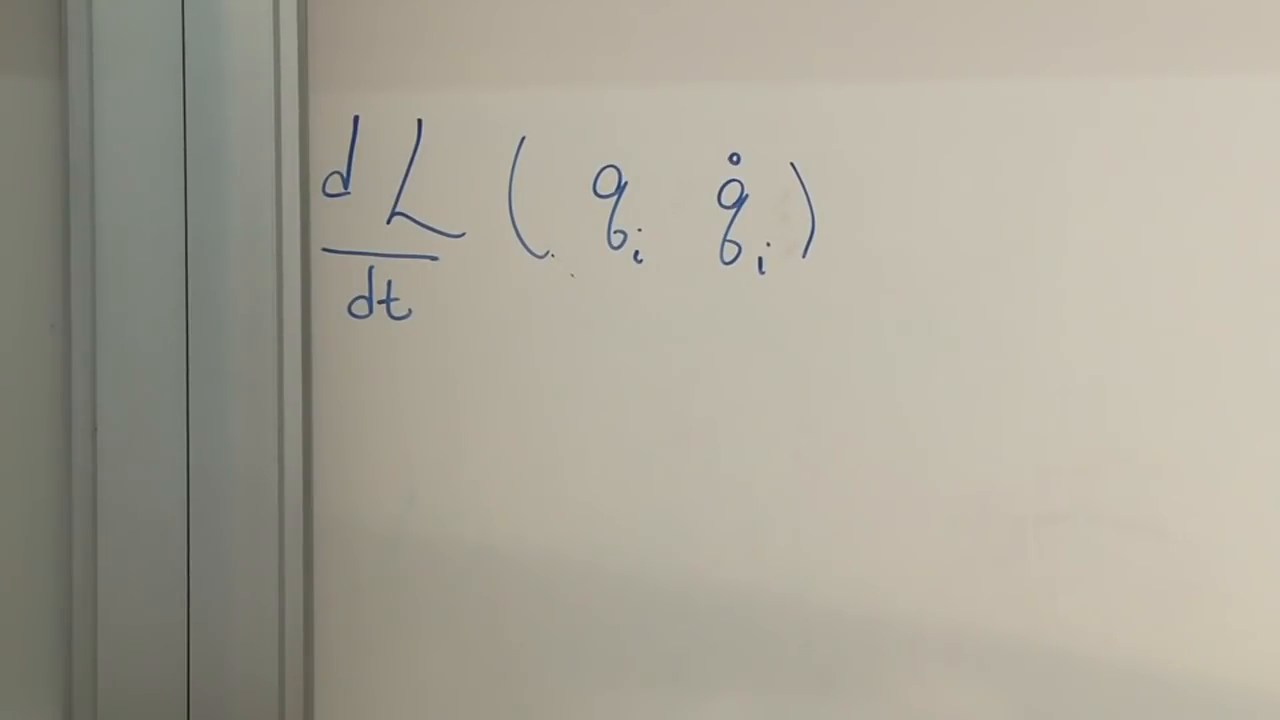
\includegraphics[width=0.72\textwidth]{lecture_05_figure_02.png}
  \caption{Начало вычисления производной \(L(q_i,\dot q_i)\) вдоль траектории.}
  \lectureframe{01:08:51}
\end{figure}

\begin{classroomqa}
  \audiencequestion{Не отсутствует ли в выражении по правилу цепочки знак суммирования?
  \lecturetimestamp{01:10:39--01:11:05}}
  \lecturerresponse{Да.  И каждая координата, и каждая скорость могут менять лагранжиан, поэтому оба члена суммируются по \(i\).}
\end{classroomqa}

Используем канонический импульс и уравнение Эйлера--Лагранжа,
\begin{equation}
  p_i=\frac{\partial L}{\partial\dot q_i},
  \qquad
  \dot p_i=\frac{\partial L}{\partial q_i}.
  \label{eq:l5-p-and-pdot}
\end{equation}
Тогда уравнение ~\eqref{eq:l5-chain-rule-no-time} принимает вид
\begin{align}
  \frac{dL}{dt}
  &=\sum_i(\dot p_i\dot q_i+p_i\ddot q_i)
  \notag\\
  &=\frac{d}{dt}\sum_i p_i\dot q_i.
  \label{eq:l5-product-rule}
\end{align}
Вся ``магия'' — это всего лишь правило произведения.

\begin{figure}[htbp]
  \centering
  \includegraphics[width=0.84\textwidth]{lecture_05_figure_21.png}
  \caption{Правило цепочки, преобразованное с помощью уравнений движения в производную от \(\sum_i p_i\dot q_i\).}
  \lectureframe{01:13:45}
\end{figure}

\begin{classroomqa}
  \audiencequestion{Должен ли последний \(q_i\) в произведении нести одну точку или две?
  \lecturetimestamp{01:14:31--01:15:32}}
  \lecturerresponse{Внутри произведения стоит \(p_i\dot q_i\), с одной точкой.  Дифференцирование произведения дает
  \(\dot p_i\dot q_i+p_i\ddot q_i\), что и объясняет две точки в развернутом втором члене.}
\end{classroomqa}

Вычитая эти две производные, получаем сохраняющуюся комбинацию. По исторической традиции берут величину с противоположным знаком и называют её гамильтонианом:
\begin{equation}
  H=\sum_i p_i\dot q_i-L.
  \label{eq:l5-hamiltonian-definition}
\end{equation}

\begin{figure}[htbp]
  \centering
  \includegraphics[width=0.80\textwidth]{lecture_05_figure_22.png}
  \caption{Сохраняющаяся комбинация \(L-\sum_i p_i\dot q_i=-H\) и определение гамильтониана.}
  \lectureframe{01:18:05}
\end{figure}

Для одной частицы в потенциале,
\begin{equation}
  L=\frac12m\dot x^2-V(x),
  \qquad p=m\dot x.
  \label{eq:l5-particle-lagrangian}
\end{equation}
Следовательно,
\begin{align}
  H&=p\dot x-L
  \notag\\
   &=m\dot x^2-\left(\frac12m\dot x^2-V(x)\right)
  \notag\\
   &=\frac12m\dot x^2+V(x)=T+V.
  \label{eq:l5-particle-energy}
\end{align}

\begin{figure}[htbp]
  \centering
  \includegraphics[width=0.86\textwidth]{lecture_05_figure_23.png}
  \caption{Гамильтониан частицы в потенциале сводится к привычной сумме кинетической и потенциальной энергий.}
  \lectureframe{01:20:50}
\end{figure}

При выводе не предполагалась никакая конкретная форма \(L\). Поэтому уравнение~\eqref{eq:l5-hamiltonian-definition}, а не \(T+V\), является общим определением энергии в этом формализме.

\section{Явная зависимость от времени и обмен энергией}

Восстановим явную зависимость от времени в правиле цепочки:
\begin{equation}
  \frac{dL}{dt}
  =\sum_i\left(
    \frac{\partial L}{\partial q_i}\dot q_i
    +\frac{\partial L}{\partial\dot q_i}\ddot q_i
  \right)
  +\frac{\partial L}{\partial t}.
  \label{eq:l5-full-chain-rule}
\end{equation}
Левая часть есть полная производная вдоль движения. Последняя частная производная берётся при фиксированных \(q\) и \(\dot q\) и дифференцирует только внешне изменяющиеся параметры. Повторяя тот же шаг с правилом произведения, получаем
\begin{equation}
  \boxed{\frac{dH}{dt}=-\frac{\partial L}{\partial t}}.
  \label{eq:l5-hamiltonian-time}
\end{equation}

\begin{figure}[htbp]
  \centering
  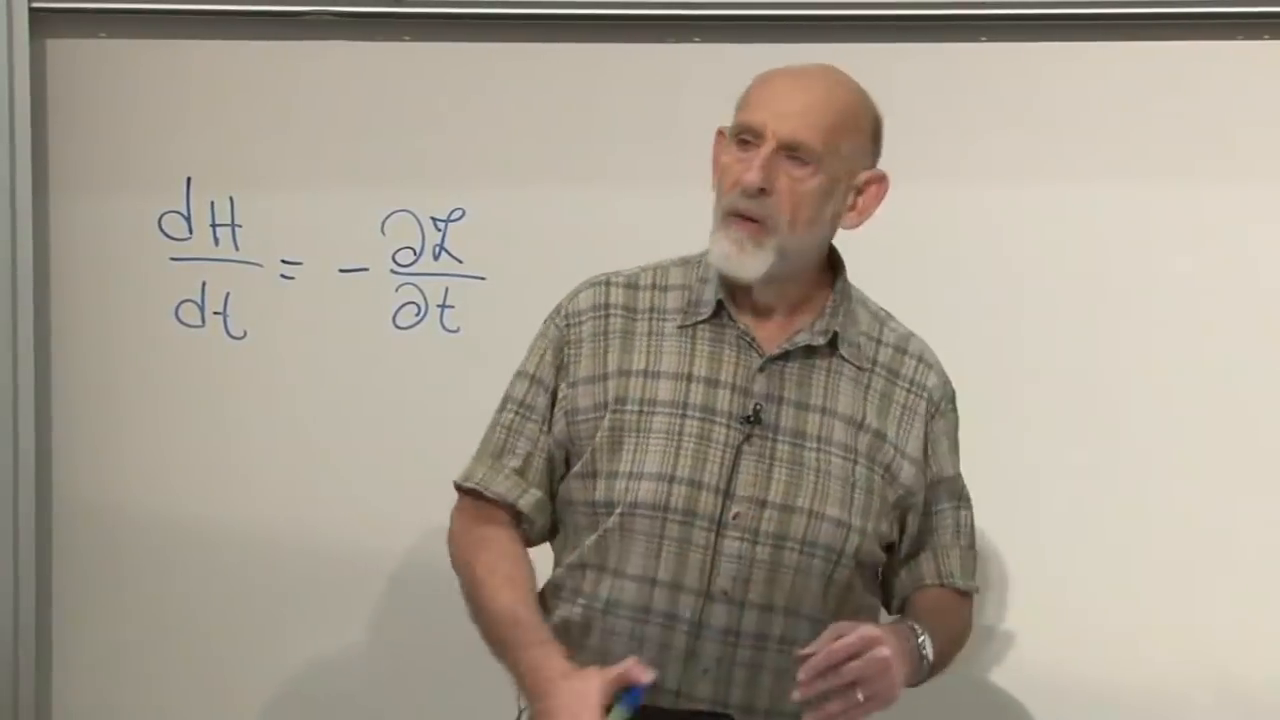
\includegraphics[width=0.70\textwidth]{lecture_05_figure_04.png}
  \caption{Гамильтониан изменяется только из-за явной зависимости лагранжиана от времени.}
  \lectureframe{01:37:22}
\end{figure}

Для вынужденного осциллятора из уравнения~\eqref{eq:l5-driven-oscillator},
\begin{equation}
  \frac{\partial L}{\partial t}
  =-\frac12\dot k(t)x^2,
  \qquad
  \dot H=\frac12\dot k(t)x^2.
  \label{eq:l5-driven-energy-rate}
\end{equation}
При \(x=0\) мгновенная производная обращается в нуль; вне начала координат изменение жёсткости пружины совершает работу с мощностью, пропорциональной \(x^2\dot k\).

\begin{classroomqa}
  \audiencequestion{Если энергия не сохраняется, не является ли её определением производная гамильтониана по времени?
  \lecturetimestamp{01:27:11--01:28:04}}
  \lecturerresponse{Нет. Энергия — это \(H\). Производная этой величины показывает, как она меняется. Когда лагранжиан имеет привычный вид, \(H=T+V\); когда нет, определение задаётся уравнением~\eqref{eq:l5-hamiltonian-definition}. Если расширить систему, включив внешний источник, восстановится сохранение полного гамильтониана.}
\end{classroomqa}

\begin{classroomqa}
  \audiencequestion{Как это применить к рассмотренному ранее наблюдателю на вращающейся карусели, где появились центробежные и кориолисовы члены?
  \lecturetimestamp{01:28:08--01:29:52}}
  \lecturerresponse{Равномерно вращающаяся система координат — это зависящая от времени замена переменных, а не фиксированная пространственная симметрия и не простой сдвиг по времени. Её преобразованный лагранжиан можно использовать для построения гамильтониана, но этот отдельный расчёт лучше отложить до обсуждения магнитных сил, поскольку соответствующая алгебра имеет очень близкую форму.}
\end{classroomqa}

\section{Лагранжев инструментарий в одном месте}

Теперь всю структуру можно записать в виде компактного набора:
\begin{align}
  L&=L(q_i,\dot q_i,t),
  \notag\\
  p_i&=\frac{\partial L}{\partial\dot q_i},
  \qquad
  \dot p_i=\frac{\partial L}{\partial q_i},
  \notag\\
  \delta q_i&=\epsilon f_i(q)
  \quad\Longrightarrow\quad
  Q=\sum_i p_i f_i(q),\quad \dot Q=0,
  \notag\\
  H&=\sum_i p_i\dot q_i-L,
  \qquad
  \dot H=-\frac{\partial L}{\partial t}.
  \label{eq:l5-toolkit}
\end{align}

\begin{figure}[htbp]
  \centering
  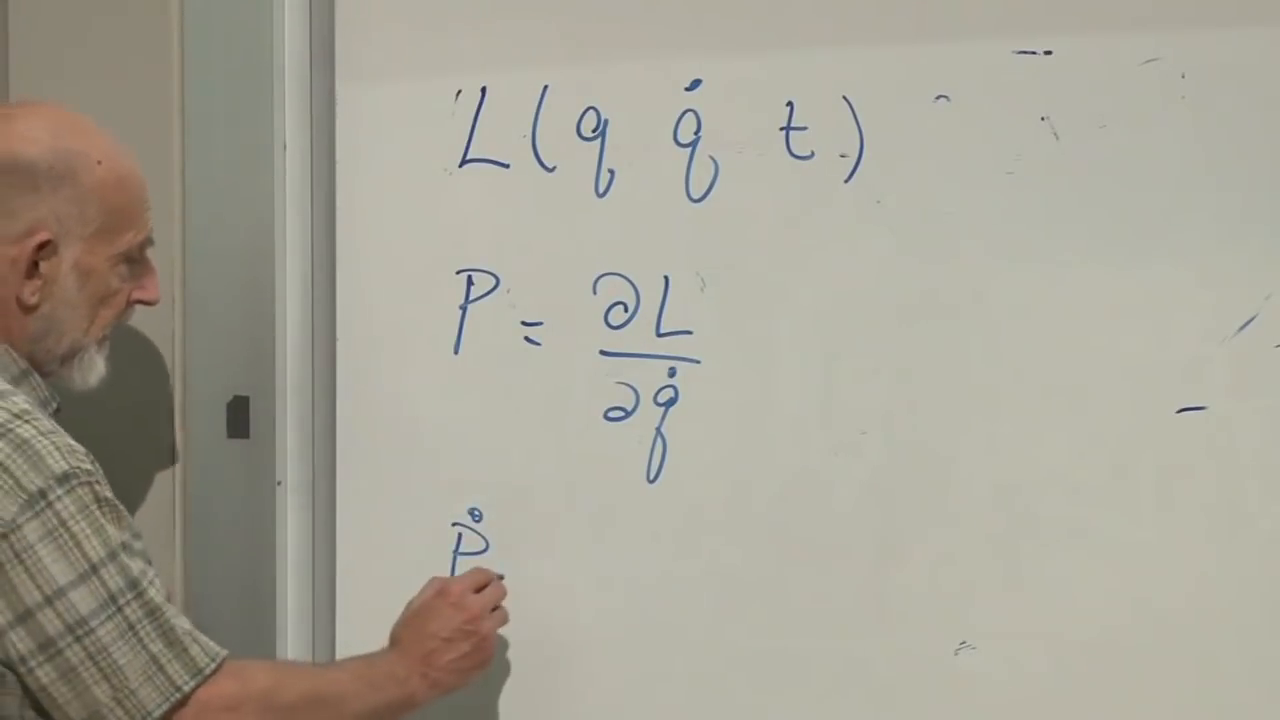
\includegraphics[width=0.66\textwidth]{lecture_05_figure_03.png}
  \caption{Краткое резюме на доске начинается с \(L(q,\dot q,t)\), канонического импульса и уравнения Эйлера--Лагранжа.}
  \lectureframe{01:31:37}
\end{figure}

Эти формулы содержат определение, уравнения движения, заряд обычной непрерывной симметрии и заряд трансляции по времени. Здесь почти нет хитростей; важно уметь заново выводить их, а не заучивать разрозненные выражения.

\section{Зачем использовать лагранжеву или гамильтонову механику?}

\begin{classroomqa}
  \audiencequestion{Можно ли в равной мере описывать механику с помощью \(L\) или \(H\), и почему выбирать ту или иную формулировку?
  \lecturetimestamp{01:37:16--01:39:18}}
  \lecturerresponse{Они эквивалентны, когда преобразование Лежандра регулярно, но подчёркивают разные структуры. Лагранжева механика естественно начинается с принципа стационарного действия. Гамильтонова механика поначалу более абстрактна, но её уравнения просты, и в квантовой механике она становится центральной. Гамильтониан — это энергия, но его роль гораздо шире, чем один только закон сохранения.}
\end{classroomqa}

\begin{classroomqa}
  \audiencequestion{Знал ли Ньютон гамильтонову форму закона сохранения энергии?
  \lecturetimestamp{01:39:29--01:39:56}}
  \lecturerresponse{Судя по историческим свидетельствам, не в этой формулировке. Ньютон формулировал механику на основе закона силы \(F=ma\).}
\end{classroomqa}

\begin{classroomqa}
  \audiencequestion{Почему всякая физическая система должна обладать лагранжианом? Это просто экспериментальный факт?
  \lecturetimestamp{01:39:57--01:42:37}}
  \lecturerresponse{Для рассматриваемых замкнутых систем это эмпирический факт и, кроме того, следствие более глубокого квантового описания. Можно придумать математически непротиворечивые дифференциальные уравнения, которые не являются уравнениями Эйлера--Лагранжа. Например, \(\dot x=-x\) прекрасно решается, но как фундаментальный закон для замкнутой системы с одной координатой оно имеет диссипативный характер с потерей информации. Классическая механика не предшествует квантовой механике логически; её фундаментальная структура унаследована от квантовой механики. Подробное объяснение придётся отложить.}
\end{classroomqa}

\begin{classroomqa}
  \audiencequestion{Если у всякой реальной замкнутой системы есть лагранжиан, то соответствует ли каждая функция, которую мы называем лагранжианом, системе, встречающейся в природе?
  \lecturetimestamp{01:42:39--01:42:54}}
  \lecturerresponse{Нет. Формальное исчисление допускает много функций, которые не реализуются ни в одной известной физической системе.}
\end{classroomqa}

\begin{classroomqa}
  \audiencequestion{Является ли лагранжиан главным образом инструментом для придумывания потенциалов?
  \lecturetimestamp{01:42:54--01:43:32}}
  \lecturerresponse{Его роль шире. Он может служить для систематизации возможных механических систем и часто является кратчайшим практическим путём к уравнениям движения.}
\end{classroomqa}

Двойной маятник демонстрирует это практическое преимущество. Выберите два угла, вычислите скорости обеих масс через эти углы и их производные по времени, составьте \(T-V\), и пусть уравнения Эйлера--Лагранжа неявно учтут силы связи. Это значительно чище, чем разбирать все натяжения и ускорения с помощью \(F=ma\).

\begin{figure}[htbp]
  \centering
  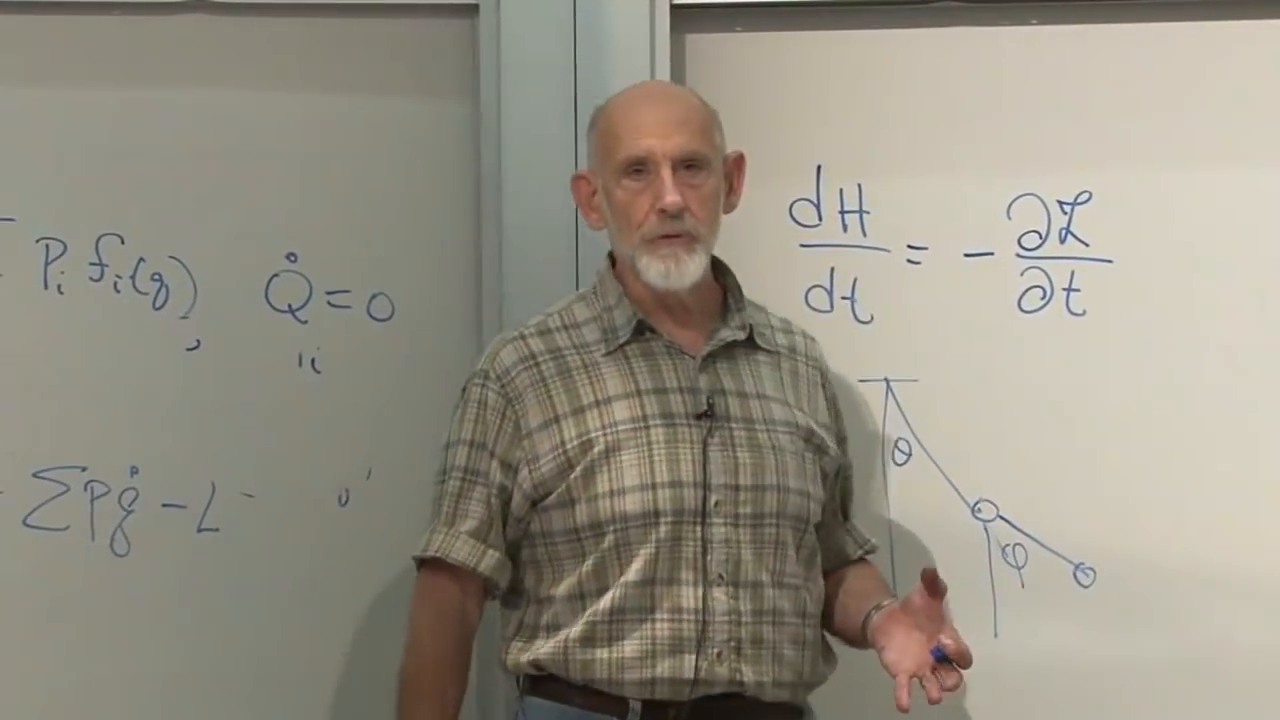
\includegraphics[width=0.84\textwidth]{lecture_05_figure_05.png}
  \caption{Соотношение для скорости изменения энергии остаётся на доске рядом с рисунком двойного маятника.}
  \lectureframe{01:45:39}
\end{figure}

\begin{figure}[htbp]
  \centering
  \begin{tikzpicture}[scale=1.15]
    \draw[thick] (-0.5,0) -- (0.5,0);
    \fill (0,0) circle (0.045);
    \draw[dashed] (0,0) -- (0,-2.3);
    \draw[thick] (0,0) -- (-0.92,-1.22);
    \fill (-0.92,-1.22) circle (0.07);
    \draw[dashed] (-0.92,-1.22) -- (-0.92,-2.55);
    \draw[thick] (-0.92,-1.22) -- (-0.25,-2.18);
    \fill (-0.25,-2.18) circle (0.07);
    \draw (0,-0.55) arc (-90:-127:0.55);
    \node at (-0.42,-0.56) {$\theta$};
    \draw (-0.92,-1.72) arc (-90:-55:0.48);
    \node at (-0.56,-1.72) {$\phi$};
  \end{tikzpicture}
  \caption{Обобщённые угловые координаты двойного маятника.}
\end{figure}

Замена переменных столь же эффективна: преобразуйте один лагранжиан, а затем выведите его уравнения, вместо того чтобы по отдельности преобразовывать каждое уравнение в терминах сил.

\begin{classroomqa}
  \audiencequestion{Является ли двойной маятник по существу ещё одной системой трёх тел, такой как Солнце, Земля и Луна, где одно тело рассматривается как опора?
  \lecturetimestamp{01:45:06--01:45:25}}
  \lecturerresponse{Эта аналогия передаёт иерархию, хотя стержни накладывают другие связи. В обоих случаях очень массивную или закреплённую составляющую можно в приближении рассматривать как опорную структуру.}
\end{classroomqa}

\begin{classroomqa}
  \audiencequestion{В двойном маятнике используется \(T-V\), хотя только что подчёркивалась важность более общих лагранжианов. Когда справедливо \(T-V\)?
  \lecturetimestamp{01:46:08--01:46:58}}
  \lecturerresponse{Для обычных нерелятивистских частиц в инерциальной системе отсчёта, при отсутствии магнитной связи, зависящей от скорости, применима привычная форма. Вращающиеся системы отсчёта, релятивистские системы и магнитные поля требуют более общих членов.}
\end{classroomqa}

\begin{classroomqa}
  \audiencequestion{Выходят ли столкновения за пределы этого описания?
  \lecturetimestamp{01:47:00--01:48:05}}
  \lecturerresponse{Упругие столкновения возникают из-за короткодействующих сил и, следовательно, из потенциалов. Неупругие столкновения на микроскопическом уровне всё равно остаются механическими, но энергия уходит во внутренние колебания, деформацию и тепло. Описание через центр масс, опускающее эти степени свободы, неполно.}
\end{classroomqa}

\begin{classroomqa}
  \audiencequestion{Можно ли анализировать бейсбольный мяч, по которому ударили битой, с помощью \(F=ma\)?
  \lecturetimestamp{01:48:05--01:48:33}}
  \lecturerresponse{Лишь на грубом уровне. Полное описание должно отслеживать деформацию, нагрев, возможное повреждение мяча и, возможно, поломку биты. Именно из-за этих внутренних степеней свободы реалистичный удар намного сложнее, чем столкновение точечных частиц.}
\end{classroomqa}

\begin{classroomqa}
  \audiencequestion{А как насчёт протяжённого твёрдого тела?
  \lecturetimestamp{01:48:34--01:49:00}}
  \lecturerresponse{Твёрдые тела можно изучать либо ньютоновскими методами, либо с помощью лагранжиана \(T-V\), записанного в поступательных и вращательных координатах. Построение такого лагранжиана — полезное упражнение.}
\end{classroomqa}

\begin{classroomqa}
  \audiencequestion{Означает ли квантовое соотношение неопределённостей энергия--время, что энергия не сохраняется строго?
  \lecturetimestamp{01:49:01--01:49:29}}
  \lecturerresponse{Нет. Энергия может сохраняться строго. Это соотношение говорит, что для определения энергии с высокой точностью требуется наблюдение в течение длительного времени; оно не заменяет закон сохранения.}
\end{classroomqa}

\begin{classroomqa}
  \audiencequestion{Ньютонова и лагранжева механика логически эквивалентны?
  \lecturetimestamp{01:49:36--01:50:07}}
  \lecturerresponse{Они эквивалентны в обычной области, где применимы обе формулировки. Тем не менее можно построить лагранжианы, чьи уравнения не похожи на элементарную форму \(m\ddot x=F(x)\).}
\end{classroomqa}

\section{Кинетический член с координатной зависимостью}

Рассмотрим намеренно непривычный пример
\begin{equation}
  L=\frac12q^2\dot q^2-\frac12q^2.
  \label{eq:l5-nonstandard-l}
\end{equation}
Это корректный лагранжиан с зависящим от координаты коэффициентом при кинетическом члене. Можно было бы рассмотреть и члены, линейные по скорости, такие как \(q\dot q\); в этом одномерном примере данный член является полной производной и не изменил бы уравнения движения.

Канонический импульс равен
\begin{equation}
  p=\frac{\partial L}{\partial\dot q}=q^2\dot q,
  \label{eq:l5-nonstandard-p}
\end{equation}
так что
\begin{equation}
  \dot p=q^2\ddot q+2q\dot q^2,
  \qquad
  \frac{\partial L}{\partial q}=q\dot q^2-q.
  \label{eq:l5-nonstandard-derivatives}
\end{equation}
Поэтому уравнение движения имеет вид
\begin{equation}
  q^2\ddot q+q\dot q^2=-q.
  \label{eq:l5-nonstandard-eom}
\end{equation}

\begin{figure}[htbp]
  \centering
  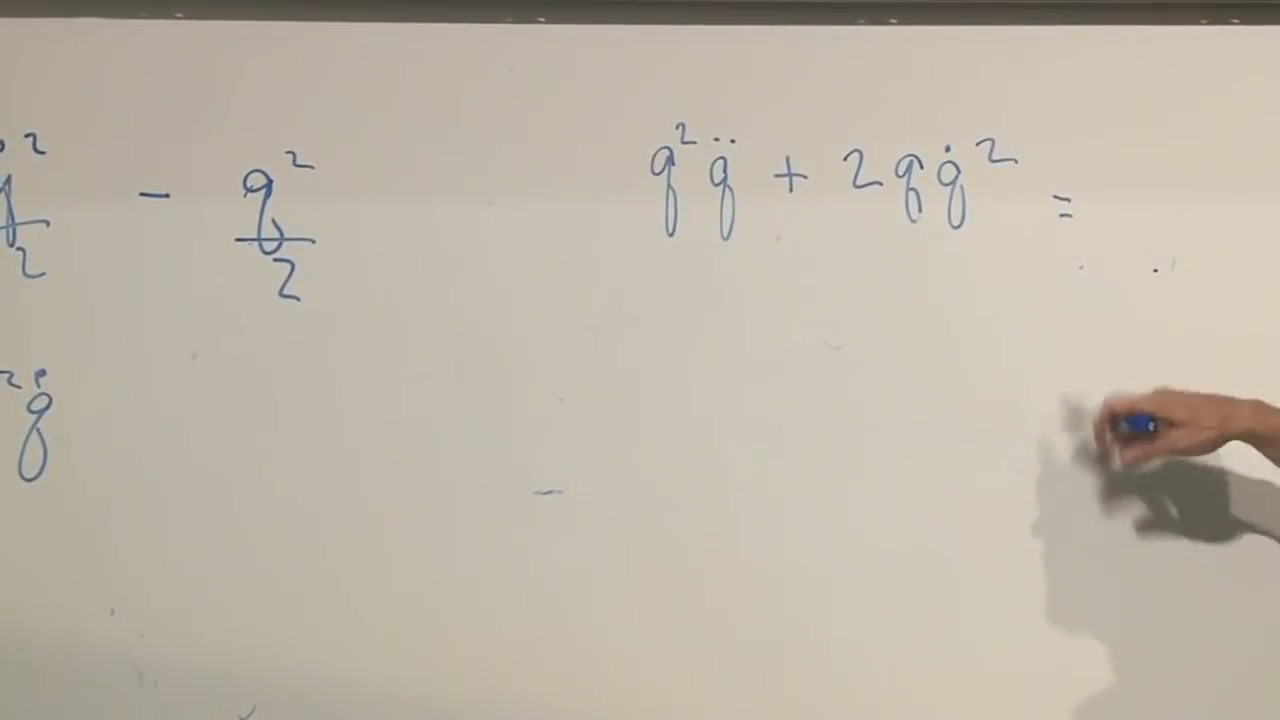
\includegraphics[width=0.80\textwidth]{lecture_05_figure_06.png}
  \caption{Производная импульса в примере с зависящим от координаты коэффициентом при кинетическом члене.}
  \lectureframe{01:52:32}
\end{figure}

\begin{classroomqa}
  \audiencequestion{Можно ли разделить уравнение на \(q\)?
  \lecturetimestamp{01:53:22--01:53:39}}
  \lecturerresponse{Только там, где \(q\neq0\). При \(q=0\) кинетический коэффициент и отображение Лежандра вырождены, поэтому деление отбросило бы особую точку, требующую отдельного рассмотрения.}
\end{classroomqa}

Гамильтониан равен
\begin{align}
  H&=p\dot q-L
  \notag\\
   &=q^2\dot q^2-
     \left(\frac12q^2\dot q^2-\frac12q^2\right)
  \notag\\
   &=\frac12q^2\dot q^2+\frac12q^2.
  \label{eq:l5-nonstandard-h}
\end{align}

\begin{classroomqa}
  \audiencequestion{Можно ли по-прежнему называть \(q^2\dot q^2/2\) кинетической энергией?
  \lecturetimestamp{01:54:41--01:55:07}}
  \lecturerresponse{Да. В этом разобранном примере гамильтониан снова выглядит как сумма положительного кинетического члена и потенциального члена. Суть в том, что формальные определения сработали без предварительного предположения о простейшей форме с постоянной массой.}
\end{classroomqa}

\section{Диссипация и более глубокое происхождение формализма}

\begin{classroomqa}
  \audiencequestion{Как включить трение в лагранжиан?
  \lecturetimestamp{01:55:09--01:56:17}}
  \lecturerresponse{Не в качестве фундаментальной силы в рассматриваемой здесь простой замкнутой системе с конечным числом степеней свободы. Макроскопическое трение представляет собой статистический эффект огромного числа микроскопических степеней свободы. Эти атомы по-прежнему подчиняются лежащей в основе механике, но в редуцированном описании, которое их не отслеживает, проявляется диссипация.}
\end{classroomqa}

\begin{classroomqa}
  \audiencequestion{Как Hamilton пришёл к своей формулировке?
  \lecturetimestamp{01:56:22--01:56:37}}
  \lecturerresponse{Здесь не приводилось исторического вывода. Важная задача для данного курса — понять, как работает эта формулировка.}
\end{classroomqa}

\begin{classroomqa}
  \audiencequestion{Есть ли более общий рецепт получения лагранжиана, когда он не имеет очевидного вида \(T-V\)?
  \lecturetimestamp{01:56:43--01:58:54}}
  \lecturerresponse{Эту функцию могут дать эксперимент, обоснованная догадка, принцип симметрии или восстановление из желаемых уравнений. Спрашивать у самого исчисления, откуда берётся его вход, — всё равно что спрашивать у определения производной, откуда взялась \(f(x)\). Исчисление говорит, что делать, когда функция уже задана. На более глубоком уровне на вопрос о том, почему замкнутые системы природы подчиняются этой абстрактной структуре, отвечает квантовая механика.}
\end{classroomqa}

Этот момент связан с темами, затронутыми в начале курса. Фундаментальная гамильтонова эволюция детерминистична и обратима в том смысле, что траектории не сливаются и информация не просто уничтожается. Связь между этим свойством и формулировкой в фазовом пространстве будет раскрываться постепенно.

\begin{classroomqa}
  \audiencequestion{Не сводилось ли вариационное исчисление просто к обратному ходу от желаемых классических уравнений, и получает ли квантовая механика свой лагранжиан тем же путём?
  \lecturetimestamp{01:59:37--02:01:07}}
  \lecturerresponse{В элементарном классическом построении действительно можно выбрать действие, стационарные траектории которого воспроизводят известные уравнения. Логический порядок в квантовой механике иной: она естественным образом начинается с гамильтониана и может переходить к лагранжеву описанию. Гамильтониан там более интуитивен, хотя в классической механике поначалу кажется абстрактным.}
\end{classroomqa}

\begin{classroomqa}
  \audiencequestion{Может ли квантовая механика описывать трение?
  \lecturetimestamp{02:01:08--02:02:05}}
  \lecturerresponse{Да, но фундаментальное описание должно включать степени свободы окружения. Частицу, движущуюся в вязкой жидкости, невозможно полностью описать без частиц самой жидкости. Трение — это сложный коллективный эффект, возникающий, когда за этими степенями свободы не следят по отдельности.}
\end{classroomqa}
\chapter{Системы со связями и гамильтоново движение}

\lectureoverview{Две системы со связями показывают, почему механика Лагранжа настолько эффективна: как только выбраны подходящие координаты, уравнения движения и соответствующие законы сохранения следуют без явного вычисления сил связи. Эти же примеры затем подводят к гамильтоновой механике, в которой координаты и импульсы образуют фазовое пространство, гармонический осциллятор превращается в жёсткое вращение, а два уравнения Гамильтона первого порядка заменяют каждое уравнение Эйлера--Лагранжа второго порядка.}

\section{Что значит решить механическую задачу}

Непосредственная цель метода Лагранжа — практическая. Клин, скользящий по полу, и двойной маятник можно рассматривать и с помощью законов Ньютона, но неизвестные силы контакта и натяжения быстро делают вычислительный учёт громоздким. Когда правила механики Лагранжа уже известны, те же задачи сводятся к последовательности чётко определённых шагов:
\begin{enumerate}
  \item выбрать независимые координаты, задающие мгновенную конфигурацию;
  \item выразить кинетическую и потенциальную энергии через эти координаты;
  \item составить \(L=T-V\) и применить уравнения Эйлера--Лагранжа.
\end{enumerate}

Для наших целей задача уже \emph{решена}, когда её уравнения движения записаны правильно. Можно по-прежнему хотеть получить траекторию в замкнутой форме, но это уже отдельный вопрос. Нелинейные дифференциальные уравнения можно интегрировать численно, как только механическая постановка завершена. Трудная часть часто состоит не в интегрировании; она состоит в том, чтобы найти переменные, которые учитывают связи, не вводя избыточных неизвестных сил.

\section{Частица, скользящая по движущемуся клину}

Рассмотрим клин массы \(M\), которому разрешено без трения скользить вдоль горизонтальной плоскости. Точечная частица массы \(m\) обязана оставаться на наклонной грани. Здесь две степени свободы: одна задаёт положение клина, а другая — положение частицы на клине.

Пусть
\begin{equation}
  \begin{aligned}
    X&=\text{horizontal position of the wedge corner},\\
    x&=\text{horizontal displacement of the particle}\\[-0.2em]
     &\phantom{={}}\text{from that corner}.
  \end{aligned}
  \label{eq:l6-wedge-coordinates}
\end{equation}
Тогда абсолютная горизонтальная координата частицы равна \(X+x\). Этот выбор не единственный. Вместо него можно было бы использовать расстояние вдоль наклонной плоскости или абсолютную горизонтальную координату частицы. Допустима любая неизбыточная пара, задающая те же конфигурации, хотя одни пары выявляют структуру яснее, чем другие.

При фиксированном угле наклона \(\beta\) вертикальное смещение \(y\) не является независимой координатой:
\begin{equation}
  y=x\tan\beta,
  \qquad
  \dot y=\dot x\tan\beta.
  \label{eq:l6-wedge-constraint}
\end{equation}
Мы специализируемся на случае \(\beta=45^\circ\), так что \(y=x\) и
\(\dot y=\dot x\). Это упрощение убирает тригонометрические множители, не меняя сути примера.

\begin{figure}[htbp]
  \centering
  \includegraphics[width=0.84\textwidth]{lecture_06_figure_06.png}
  \caption{Движущийся клин, связанная частица и горизонтальная и вертикальная компоненты скорости, используемые в примере с \(45^\circ\).}
  \lectureframe{00:10:25}
\end{figure}

Кинетическая энергия клина равна
\begin{equation}
  T_{M}=\frac{M}{2}\dot X^2.
  \label{eq:l6-wedge-kinetic}
\end{equation}
Горизонтальная скорость частицы равна \(\dot X+\dot x\), а её вертикальная скорость — \(\dot x\). Поэтому её кинетическая энергия равна
\begin{equation}
  T_m=\frac{m}{2}\left[(\dot X+\dot x)^2+\dot x^2\right].
  \label{eq:l6-particle-kinetic}
\end{equation}
Выбрав нуль гравитационной потенциальной энергии при \(x=0\), получаем \(V=mgx\).
Следовательно,
\begin{equation}
  L=\frac{M}{2}\dot X^2
    +\frac{m}{2}\left[(\dot X+\dot x)^2+\dot x^2\right]
    -mgx.
  \label{eq:l6-wedge-lagrangian}
\end{equation}

\begin{figure}[htbp]
  \centering
  \includegraphics[width=0.86\textwidth]{lecture_06_figure_07.png}
  \caption{Геометрия клина, \(V=mgx\) и два вклада в кинетическую энергию, собранные на доске.}
  \lectureframe{00:14:15}
\end{figure}

\subsection{Канонический импульс определяется лагранжианом}

Канонические импульсы определяются лагранжианом, а не догадкой, основанной на скорости отдельной частицы:
\begin{align}
  p_X&=\frac{\partial L}{\partial\dot X}
      =M\dot X+m(\dot X+\dot x),
      \label{eq:l6-wedge-pX}\\
  p_x&=\frac{\partial L}{\partial\dot x}
      =m(\dot X+\dot x)+m\dot x.
      \label{eq:l6-wedge-px}
\end{align}
Первое выражение — это обычный полный горизонтальный импульс: клин даёт вклад \(M\dot X\), а частица даёт вклад
\(m(\dot X+\dot x)\). Здесь он появляется как импульс, сопряжённый координате \(X\).

\begin{figure}[htbp]
  \centering
  \includegraphics[width=0.86\textwidth]{lecture_06_figure_08.png}
  \caption{Канонические импульсы, сопряжённые координате клина \(X\) и относительной координате частицы \(x\).}
  \lectureframe{00:18:05}
\end{figure}

Лагранжиан не зависит явно от \(X\). Горизонтальный перенос всей установки действует как
\begin{equation}
  \delta X=\epsilon,
  \qquad
  \delta x=0.
  \label{eq:l6-wedge-translation}
\end{equation}
Общее правило для бесконечно малого преобразования симметрии
\begin{equation}
  \delta q_i=\epsilon f_i(q),
  \qquad
  Q=\sum_i p_i f_i
  \label{eq:l6-noether-rule}
\end{equation}
поэтому даёт \(Q=p_X\). Эквивалентно, \(X\) является циклической координатой, и
\begin{equation}
  \dot p_X=\frac{\partial L}{\partial X}=0.
  \label{eq:l6-wedge-conservation}
\end{equation}

Соответствующей симметрии вертикального переноса нет. Клин не может двигаться по вертикали, а изменение высоты частицы меняет гравитационную потенциальную энергию. Горизонтальный импульс сохраняется; вертикальный импульс этой подсистемы со связями — нет.

Для относительной координаты уравнение Эйлера--Лагранжа имеет вид
\begin{equation}
  \dot p_x=\frac{\partial L}{\partial x}=-mg.
  \label{eq:l6-wedge-force}
\end{equation}
Эта строка на доске потребовала исправления знака. Надёжный путь — начать с \(L=T-V\): поскольку \(V=mgx\), производная лагранжиана равна
\(-mg\). То, что \(x\) была введена как горизонтальное смещение, не устраняет гравитацию из её уравнения, потому что связь привязывает это горизонтальное смещение к вертикальной высоте \(y=x\).

Никакая нормальная сила или сила реакции здесь не появилась. Такие силы принимают ровно те значения, которые необходимы для поддержания связей. Метод Ньютона ввёл бы их и определял вместе с ускорениями; обобщённые координаты сделали их ненужными.

\section{Двойной маятник и искусство выбора координат}

Теперь подвесим две единичные массы на двух невесомых стержнях единичной длины. Первый стержень образует угол \(\theta\) с вертикалью, направленной вниз. Для второй степени свободы у нас есть выбор. Можно использовать второй абсолютный угол \(\phi\), а можно — относительный угол \(\alpha\) между стержнями.

Относительный угол — более показательный выбор. Временно выключим гравитацию. Жёсткий поворот всей установки меняет абсолютную ориентацию, но не угол между стержнями:
\begin{equation}
  \theta\longrightarrow\theta+\epsilon,
  \qquad
  \alpha\longrightarrow\alpha.
  \label{eq:l6-double-rotation}
\end{equation}
При таком выборе вращательная симметрия действует только на одну координату. Это не делает другие системы координат неправильными. Просто так легче увидеть симметрию и, следовательно, сохраняющуюся величину.

\begin{figure}[htbp]
  \centering
  \includegraphics[width=0.76\textwidth]{lecture_06_figure_09.png}
  \caption{Двойной маятник, в котором \(\theta\) — первый абсолютный угол, а
  \(\alpha\) — угол второго стержня относительно первого.}
  \lectureframe{00:29:20}
\end{figure}

Чтобы получить кинетическую энергию, используем декартовы координаты как временное вспомогательное средство учёта. Если вертикальная координата отсчитывается вниз, то первый грузик находится в точке
\begin{equation}
  x_1=\sin\theta,
  \qquad
  y_1=\cos\theta,
  \label{eq:l6-bob-one-position}
\end{equation}
и потому
\begin{equation}
  \dot x_1=\dot\theta\cos\theta,
  \qquad
  \dot y_1=-\dot\theta\sin\theta,
  \qquad
  \dot x_1^2+\dot y_1^2=\dot\theta^2.
  \label{eq:l6-bob-one-velocity}
\end{equation}
Второй грузик находится в точке
\begin{align}
  x_2&=\sin\theta+\sin(\theta+\alpha),\\
  y_2&=\cos\theta+\cos(\theta+\alpha),
  \label{eq:l6-bob-two-position}
\end{align}
так что, например,
\begin{equation}
  \dot x_2=\dot\theta\cos\theta
  +(\dot\theta+\dot\alpha)\cos(\theta+\alpha),
  \label{eq:l6-bob-two-xvelocity}
\end{equation}
причём для \(\dot y_2\) получается аналогичное выражение.

\begin{figure}[htbp]
  \centering
  \includegraphics[width=0.88\textwidth]{lecture_06_figure_10.png}
  \caption{Вспомогательные декартовы координаты для двух грузиков. Они используются
  для вычисления скоростей, а не вводятся как дополнительные степени свободы.}
  \lectureframe{00:35:25}
\end{figure}

Сложение двух кинетических энергий даёт согласованный результат, приведённый ниже. Перекрёстный член следует из
\begin{equation*}
  \cos A\cos B+\sin A\sin B=\cos(A-B).
\end{equation*}
\begin{equation}
  T=\dot\theta^2
    +\frac12(\dot\theta+\dot\alpha)^2
    +\dot\theta(\dot\theta+\dot\alpha)\cos\alpha.
  \label{eq:l6-double-kinetic}
\end{equation}

\begin{classroomqa}
  \audiencequestion{Включает ли это выражение уже кинетическую энергию
  обоих грузиков, и не потерян ли множитель в одну вторую?
  \lecturetimestamp{00:38:06--00:38:27}}
  \lecturerresponse{Оно включает обе. Оно получается из
  \(\tfrac12(\dot x_1^2+\dot y_1^2+\dot x_2^2+\dot y_2^2)\).
  Два одинаковых вклада складываются в первый член
  \(\dot\theta^2\); никакой множитель не пропущен.}
\end{classroomqa}

Без гравитации \(L=T\) не содержит явной зависимости от \(\theta\). Следовательно,
\begin{equation}
  \dot p_\theta=\frac{\partial L}{\partial\theta}=0,
  \label{eq:l6-double-angular-conservation}
\end{equation}
и \(p_\theta\) — это полный угловой момент. Обратите внимание на точный смысл утверждения, что \(\theta\) не входит: \(\dot\theta\), разумеется, входит, но сама недифференцированная координата — нет.

Возвращение гравитации нарушает глобальную вращательную симметрию. Для принятого выше соглашения о вертикали, направленной вниз, один удобный выбор нуля даёт
\begin{equation}
  V=-g(y_1+y_2)
   =-g\left[2\cos\theta+\cos(\theta+\alpha)\right].
  \label{eq:l6-double-potential}
\end{equation}
Аддитивная постоянная ничего бы не изменила. Важно то, что
\(\theta\) теперь входит явно, так что сопряжённый ему импульс больше не сохраняется. Энергия по-прежнему сохраняется, потому что лагранжиан не зависит явно от времени.

\begin{classroomqa}
  \audiencequestion{Следует ли записанное на доске
  \(\dot\theta-\dot\alpha\) заменить на
  \(\dot\theta+\dot\alpha\)?
  \lecturetimestamp{00:43:00--00:43:54}}
  \lecturerresponse{Используемая здесь ориентация требует знака плюс. Это
  соглашение принято в уравнении ~\eqref{eq:l6-bob-two-position} и затем проведено
  в кинетической энергии в уравнении ~\eqref{eq:l6-double-kinetic}. Если изменить
  определение положительного \(\alpha\), соответствующие знаки изменятся, но тогда
  каждое вхождение тоже надо менять согласованно. На доске были смешаны два
  соглашения.}
\end{classroomqa}

\begin{figure}[htbp]
  \centering
  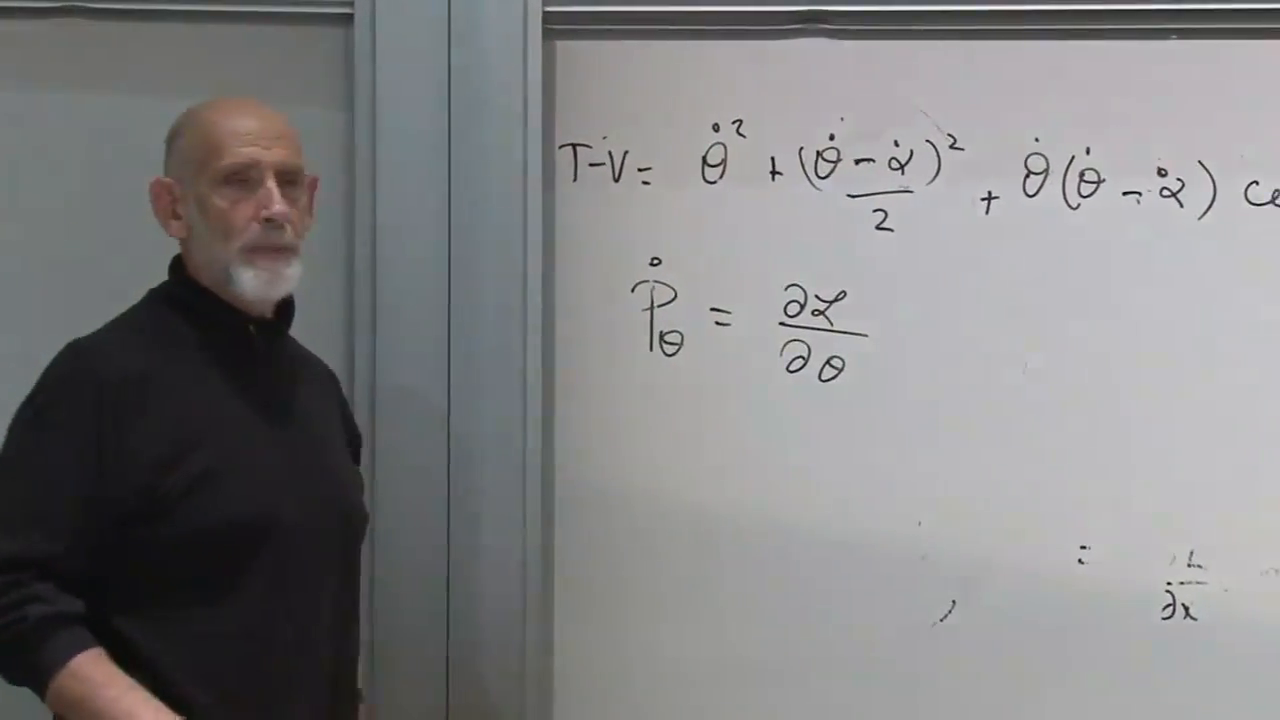
\includegraphics[width=0.84\textwidth]{lecture_06_figure_02.png}
  \caption{Вычисление для маятника без гравитации и
  \(\dot p_\theta=\partial L/\partial\theta\). Верхняя строка на доске сохраняет
  локальное обозначение с несогласованными знаками, обсуждавшееся в вопросе; нормализованная
  формула — уравнение ~\eqref{eq:l6-double-kinetic}.}
  \lectureframe{00:45:50}
\end{figure}

Как только известны \(T\) и \(V\), остальные уравнения получаются дифференцированием. Натяжения стержней и силы, обеспечивающие неизменность длин, вновь исчезли благодаря выбору координат.

\subsection{Что сохранение означает и чего не означает}

\begin{classroomqa} \audiencequestion{Можно ли непосредственно по уравнениям увидеть, хаотичен ли двойной маятник? \lecturetimestamp{00:44:57--00:45:25}} \lecturerresponse{Обычно нет, если просто смотреть на уравнения. При изменении параметров или энергии система может переходить от регулярного поведения к хаотическому. Здесь требуется больше структуры, чем дает непосредственный вид уравнений, и мы вернемся к этому позже.} \end{classroomqa}

\begin{classroomqa} \audiencequestion{В консервативной системе каждая ли \(\dot p_i\) равна нулю? \lecturetimestamp{00:45:25--00:46:24}} \lecturerresponse{Нет. Общее уравнение имеет вид \(\dot p_i=\partial L/\partial q_i\). Она обращается в нуль только тогда, когда \(q_i\) является циклической. Циклическая координата — это особенно простой случай, когда симметрия сдвигает одну координату, оставляя остальные фиксированными.} \end{classroomqa}

Если единственная цель — численно проследить эволюцию, неудобная система координат все равно годится; она лишь приводит к более длинным уравнениям. Выигрыш от удачного выбора носит концептуальный характер: сохраняющийся импульс виден еще до решения уравнений.

\begin{classroomqa} \audiencequestion{Без гравитации ведет ли себя двойной маятник так же просто, как один свободный маятник? \lecturetimestamp{00:47:02--00:47:35}} \lecturerresponse{Один свободный ротор вращается равномерно, потому что его единственный момент импульса полностью задает его движение. Двойной маятник может совершать очень сложное относительное движение, сохраняя при этом полный момент импульса. Если обе угловые скорости вначале равны нулю, система остается в покое; в противном случае две части взаимодействуют.} \end{classroomqa}

\begin{classroomqa} \audiencequestion{Являются ли \(\dot\theta\) и \(\dot\alpha\) по отдельности постоянными при отсутствии гравитации? \lecturetimestamp{00:47:36--00:52:42}} \lecturerresponse{Нет. Закон сохранения утверждает \(\dot p_\theta=0\), а не \(\ddot\theta=0\) или \(\ddot\alpha=0\). Выражение для \(p_\theta=\partial L/\partial\dot\theta\) содержит обе угловые скорости и зависит от \(\alpha\). Стержни передают моменты сил, позволяя двум грузам обмениваться моментом импульса и энергией. Это аналогично двум массам, соединенным пружиной: полный импульс и скорость центра масс постоянны, тогда как скорости каждой массы осциллируют. Вращательным аналогом здесь служит определенная коллективная комбинация, а не какой-либо из углов сам по себе.} \end{classroomqa}

\begin{classroomqa} \audiencequestion{Передаются ли через стержни силы, благодаря которым происходит обмен моментом импульса? \lecturetimestamp{00:52:43--00:53:34}} \lecturerresponse{Да. Сила, передаваемая вдоль стержня, не обязана проходить через точку подвеса другого звена, поэтому она может создавать момент силы. Момент силы — это просто вращательное действие силы, и здесь именно он приводит к ненулевым угловым ускорениям каждого звена.} \end{classroomqa}

\section{Гамильтониан как третья формулировка}

Гамильтониан — это энергия, но в этом состоит лишь его первое значение. Он также лежит в основе третьей формулировки механики. В уравнениях Ньютона используются силы и ускорения. Из принципа стационарного действия следуют уравнения Эйлера--Лагранжа. Для регулярных систем гамильтонова механика эквивалентна последним, но ее переменные и геометрия выглядят иначе.

Вместо \(q_i\) и \(\dot q_i\) используйте \(q_i\) и сопряженные с ними импульсы \(p_i\). Состояние системы с \(n\) степенями свободы требует \(2n\) чисел в любом из двух описаний: координат и скоростей либо координат и импульсов. Связь между ними задается соотношением: \begin{equation}
  p_i=\frac{\partial L}{\partial\dot q_i}.
  \label{eq:l6-legendre-map}
\end{equation} Когда эти соотношения можно обратить и выразить скорости как \(\dot q_i(q,p)\), определим \begin{equation}
  H(q,p)=\sum_i p_i\dot q_i-L(q,\dot q).
  \label{eq:l6-hamiltonian-definition}
\end{equation} Тогда скорости в правой части исключаются в пользу \(q\) и \(p\). Эта обратимость и есть предположение о регулярности преобразования Лежандра. Для сингулярных лагранжианов требуется более общая теория связей; этим элементарным построением они не охватываются.

\subsection{Обратимость до дифференциального исчисления}

Вспомним конечный набор абстрактных состояний, соединенных стрелками. Детерминистическое правило все же может оказаться необратимым, если два более ранних состояния переходят в одно более позднее. Будущее единственно, но прошлое — нет. Если обратить все стрелки, получится противоположный дефект: одно состояние ветвится в несколько будущих. На первой схеме стрелки сходятся, на второй — расходятся.

\begin{figure}[htbp] \centering
  \includegraphics[width=0.86\textwidth]{lecture_06_figure_11.png} \caption{Абстрактные отображения состояний, используемые для сопоставления обратимых циклов с запрещенными случаями схождения и расхождения.} \lectureframe{00:56:20} \end{figure}

Гамильтонов поток даст непрерывную версию этого утверждения. Облако точек фазового пространства может перемещаться и деформироваться, но не может приобрести сток, уничтожающий различия между состояниями, или источник, порождающий несколько будущих из одного состояния. Доказательство будет дано позже; пока эти диаграммы лишь мотивируют геометрию.

\begin{classroomqa} \audiencequestion{Следует ли понимать абстрактную диаграмму состояний как объект, движущийся в гравитационном поле? \lecturetimestamp{00:58:02--00:58:35}} \lecturerresponse{Нет. Точки — это всего лишь абстрактные состояния, а стрелки задают правило изменения состояния. Никакого пространственного или гравитационного смысла рисунку не приписывалось.} \end{classroomqa}

\begin{classroomqa} \audiencequestion{Чем запрещенное сходящееся отображение состояний отличается от черной дыры? \lecturetimestamp{00:58:40--00:59:28}} \lecturerresponse{Ответить можно лишь с трудом и большой осторожностью. Это уместный вопрос, но для правильного ответа требуется аккуратное описание полного состояния и его квантово-гравитационной эволюции. Элементарной диаграммы для этого недостаточно.} \end{classroomqa}

\section{Осциллятор в переменных, адаптированных к фазовому пространству}

Прежде чем выводить общие уравнения, рассмотрим гармонический осциллятор, записанный в специально подобранных переменных: \begin{equation}
  L=\frac{1}{2\omega}\dot q^2-\frac{\omega}{2}q^2.
  \label{eq:l6-rescaled-lagrangian}
\end{equation} Его сопряженный импульс равен \begin{equation}
  p=\frac{\partial L}{\partial\dot q}=\frac{\dot q}{\omega},
  \qquad
  \dot q=\omega p.
  \label{eq:l6-rescaled-momentum}
\end{equation} Подстановка в уравнение~\eqref{eq:l6-hamiltonian-definition} дает \begin{align}
  H&=p\dot q-L\\
   &=\omega p^2-\frac{\omega p^2}{2}+\frac{\omega q^2}{2}
    =\frac{\omega}{2}(p^2+q^2).
  \label{eq:l6-oscillator-hamiltonian}
\end{align}

\begin{figure}[htbp] \centering
  \includegraphics[width=0.86\textwidth]{lecture_06_figure_12.png} \caption{Преобразование Лежандра для адаптированного осциллятора и симметричный гамильтониан \(H=\tfrac{\omega}{2}(p^2+q^2)\).} \lectureframe{01:08:20} \end{figure}

Пространство переменных \(q\) и \(p\) — это фазовое пространство. Одна степень свободы дает двумерную плоскость; две степени свободы дают четырехмерное фазовое пространство. При фиксированной энергии осциллятора \begin{equation}
  p^2+q^2=\frac{2H}{\omega},
  \label{eq:l6-energy-circle}
\end{equation} поэтому траектория остается на окружности. Закон сохранения энергии ограничивает движение одной такой кривой.

\begin{figure}[htbp] \centering
  \includegraphics[width=0.82\textwidth]{lecture_06_figure_13.png} \caption{Вложенные окружности постоянной энергии на фазовой плоскости осциллятора: \(q\) по горизонтали, \(p\) по вертикали.} \lectureframe{01:13:20} \end{figure}

\section{Вывод уравнений Гамильтона}

Этот вывод — упражнение на дифференциал функции нескольких переменных. Для \(F(q,p)\) \begin{equation}
  \delta F=\sum_i\left(
  \frac{\partial F}{\partial q_i}\delta q_i
  +\frac{\partial F}{\partial p_i}\delta p_i\right).
  \label{eq:l6-total-differential}
\end{equation} Коэффициенты можно читать в обе стороны: коэффициент при \(\delta q_i\) равен \(\partial F/\partial q_i\), а коэффициент при \(\delta p_i\) равен \(\partial F/\partial p_i\).

Теперь проварьируем определяющее выражение для \(H\): \begin{align}
  \delta H
  &=\sum_i\left(\dot q_i\,\delta p_i
       +p_i\,\delta\dot q_i\right)-\delta L\\
  &=\sum_i\left(\dot q_i\,\delta p_i
       +p_i\,\delta\dot q_i
       -\frac{\partial L}{\partial q_i}\delta q_i
       -\frac{\partial L}{\partial\dot q_i}\delta\dot q_i\right).
  \label{eq:l6-vary-hamiltonian}
\end{align} Поскольку \(\partial L/\partial\dot q_i=p_i\), два члена с \(\delta\dot q_i\) сокращаются. Уравнения Эйлера--Лагранжа дают \(\partial L/\partial q_i=\dot p_i\), и остается \begin{equation}
  \delta H=\sum_i\left(\dot q_i\,\delta p_i
                     -\dot p_i\,\delta q_i\right).
  \label{eq:l6-reduced-variation}
\end{equation}

\begin{figure}[htbp] \centering
  \includegraphics[width=0.86\textwidth]{lecture_06_figure_14.png} \caption{Разложение \(\delta H\) по правилу произведения до сокращения членов \(p_i\,\delta\dot q_i\).} \lectureframe{01:18:40} \end{figure}

Сравнивая уравнение~\eqref{eq:l6-reduced-variation} с общим дифференциалом из уравнения~\eqref{eq:l6-total-differential}, из независимых коэффициентов получаем уравнения Гамильтона: \begin{equation}
  \boxed{
  \dot q_i=\frac{\partial H}{\partial p_i},
  \qquad
  \dot p_i=-\frac{\partial H}{\partial q_i}.}
  \label{eq:l6-hamilton-equations}
\end{equation}

\begin{figure}[htbp] \centering
  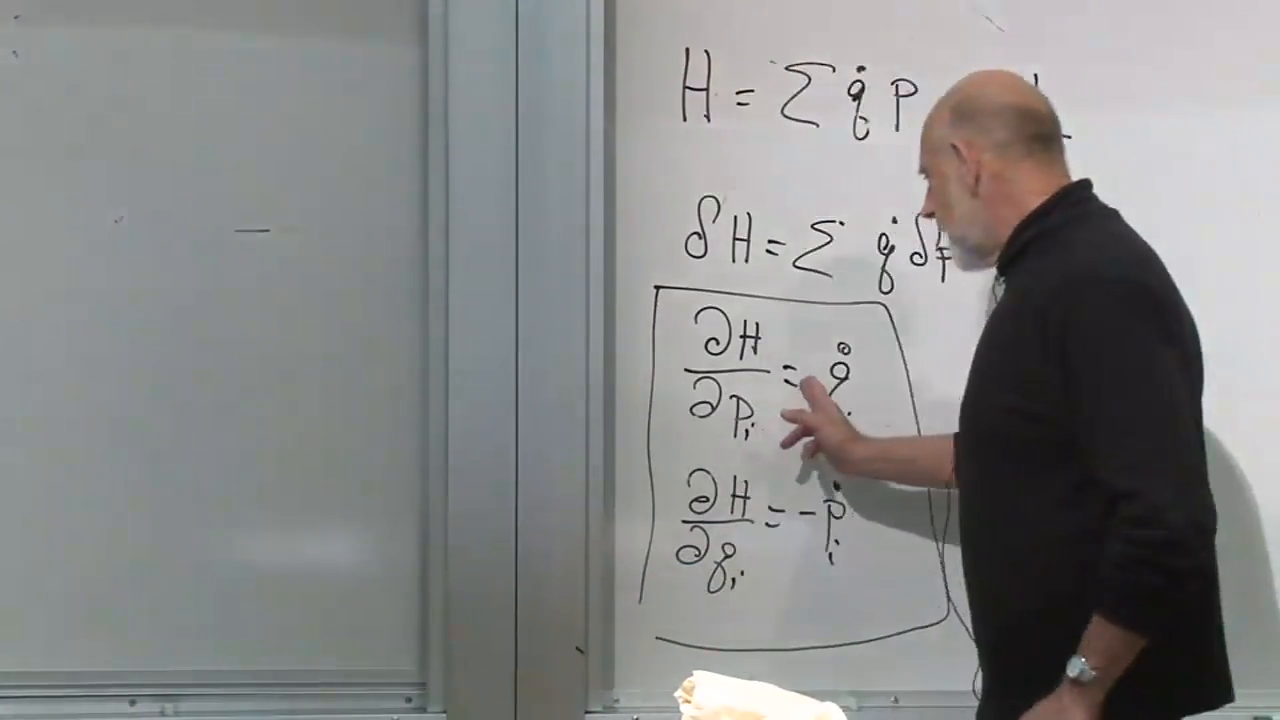
\includegraphics[width=0.78\textwidth]{lecture_06_figure_03.png} \caption{Определение гамильтониана, его вариация и выделенные в рамку канонические уравнения.} \lectureframe{01:22:18} \end{figure}

Для \(n\) координат это \(2n\) уравнений первого порядка. Формулировка Эйлера--Лагранжа, напротив, дает \(n\) уравнений второго порядка. Объем начальных данных и физическое содержание одинаковы.

\section{Движение осциллятора как жесткое вращение}

Применяя уравнения~\eqref{eq:l6-hamilton-equations} к уравнению~\eqref{eq:l6-oscillator-hamiltonian}, получаем \begin{equation}
  \dot q=\omega p,
  \qquad
  \dot p=-\omega q.
  \label{eq:l6-oscillator-first-order}
\end{equation} Дифференцируя первое уравнение и используя второе, \begin{equation}
  \ddot q=\omega\dot p=-\omega^2q.
  \label{eq:l6-oscillator-second-order}
\end{equation} Таким образом, эти два уравнения первого порядка в точности эквивалентны обычному уравнению осциллятора второго порядка вместе с определением импульса.

В фазовом пространстве вектор скорости в точке \((q,p)\) равен \((\dot q,\dot p)=(\omega p,-\omega q)\) и касателен к окружности постоянной энергии. Каждый радиус вращается с одной и той же угловой скоростью \(\omega\). Всю плоскость можно представить как жесткую вертушку или как несжимаемую фиктивную жидкость. Ее точки циркулируют; они не сжимаются в сток и не разлетаются от источника.

\begin{figure}[htbp] \centering
  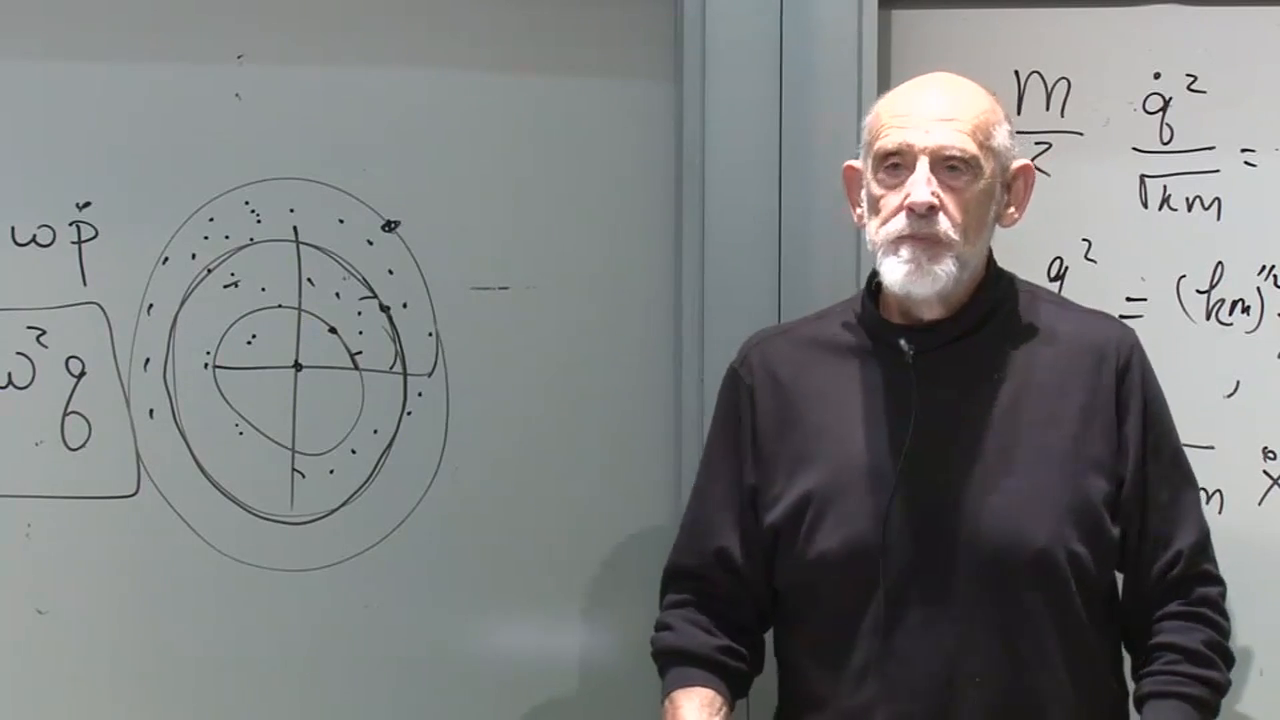
\includegraphics[width=0.86\textwidth]{lecture_06_figure_04.png} \caption{Облако начальных точек, распределенных по вложенным траекториям в фазовом пространстве. Гамильтонова эволюция перемещает это облако, а не схлопывает его в некоторое выделенное состояние.} \lectureframe{01:39:27} \end{figure}

\begin{figure}[htbp] \centering
  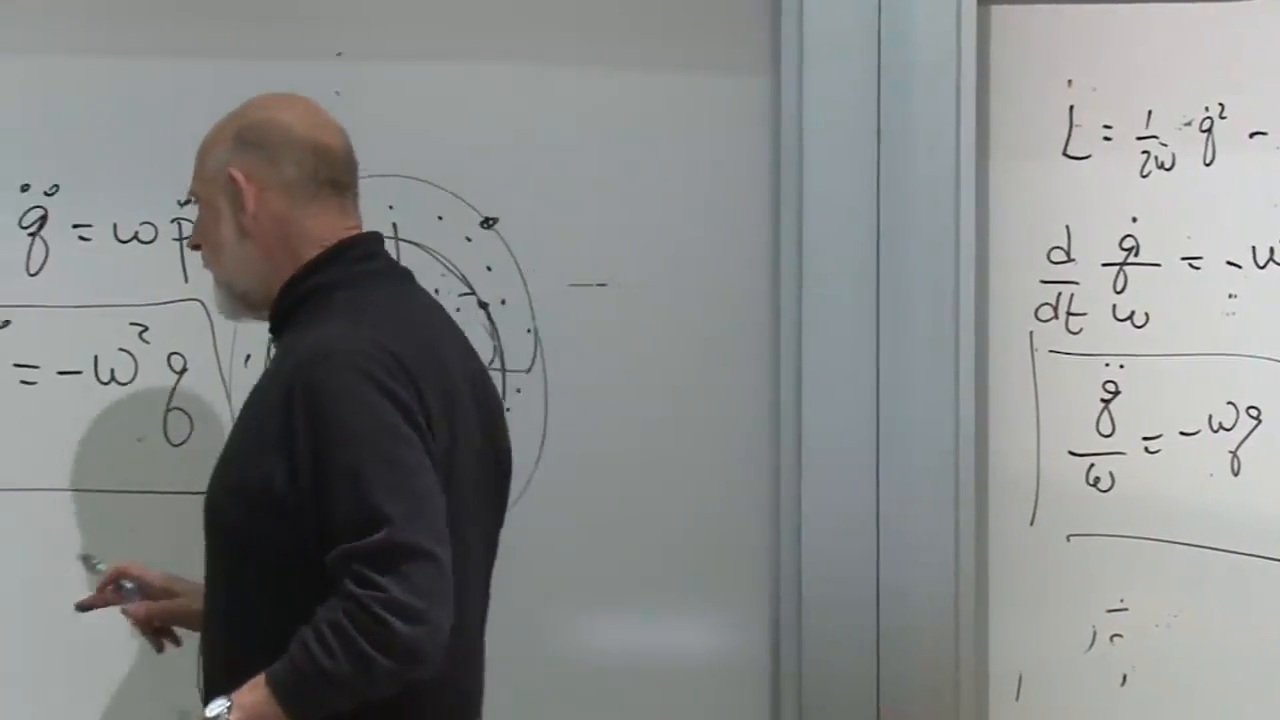
\includegraphics[width=0.90\textwidth]{lecture_06_figure_05.png} \caption{Фазовый портрет осциллятора рядом с эквивалентным уравнением Эйлера--Лагранжа \(\ddot q/\omega=-\omega q\).} \lectureframe{01:42:10} \end{figure}

Следующий шаг — превратить аналогию с жидкостью в теорему: гамильтонов поток не имеет локального схождения или расхождения. Этот результат вновь связывает непрерывную механику с обратимыми отображениями состояний, рассмотренными в начале курса.

\section{Вопросы, выявляющие выбор координат}

\begin{classroomqa}
  \audiencequestion{Является ли предположение о том, что скорости можно выразить через \(q\) и \(p\), теоремой или эмпирическим свойством физических систем?
  \lecturetimestamp{01:29:08--01:29:45}}
  \lecturerresponse{В рамках этого элементарного изложения это эмпирическая закономерность; более глубокая мотивация приходит из квантовой механики. Точнее, уравнение~\eqref{eq:l6-legendre-map} должно иметь невырожденный якобиан по скоростям. В современной механике встречаются и важные вырожденные лагранжианы, особенно системы со связями и калибровочные системы, но их гамильтонова формулировка требует дополнительного аппарата связей.}
\end{classroomqa}

Возражение, связанное с размерностями, объясняет, почему осциллятор был записан в непривычной форме уравнения~\eqref{eq:l6-rescaled-lagrangian}. Начнем вместо этого с обычной координаты \(x\):
\begin{equation}
  L=\frac{m}{2}\dot x^2-\frac{k}{2}x^2,
  \qquad
  \omega=\sqrt{\frac{k}{m}}.
  \label{eq:l6-ordinary-oscillator}
\end{equation}
Выберем
\begin{equation}
  q=(km)^{1/4}x.
  \label{eq:l6-oscillator-rescaling}
\end{equation}
Тогда \(q^2=\sqrt{km}\,x^2\) и \(\dot q^2=\sqrt{km}\,\dot x^2\), что в точности переводит уравнение~\eqref{eq:l6-ordinary-oscillator} в уравнение~\eqref{eq:l6-rescaled-lagrangian}. Новая \(q\) — это адаптированная обобщенная координата, а не длина, и сопряженная с ней \(p\) — не обычный механический импульс \(p_x=m\dot x\).

\begin{figure}[htbp]
  \centering
  \includegraphics[width=0.86\textwidth]{lecture_06_figure_15.png}
  \caption{Размерностное масштабирование от обычной координаты осциллятора \(x\) к адаптированной координате \(q=(km)^{1/4}x\).}
  \lectureframe{01:36:10}
\end{figure}

\begin{classroomqa}
  \audiencequestion{Как соотношение \(\omega p=\dot q\) может быть размерностно согласованным, и почему были выбраны эти переменные?
  \lecturetimestamp{01:29:46--01:39:22}}
  \lecturerresponse{Символ \(q\) не обязан иметь размерность длины, а сопряженный с ним \(p\) не обязан иметь размерность \(m\dot x\). Масштабирование в уравнении~\eqref{eq:l6-oscillator-rescaling} сохраняет размерность лагранжиана и заставляет \(q\) и \(p\) входить в \(H\) симметрично. В исходных переменных,
  \[
    H=\frac{p_x^2}{2m}+\frac{kx^2}{2},
  \]
  так что кривые постоянной энергии на плоскости \((x,p_x)\) являются эллипсами. На адаптированной плоскости \((q,p)\) это окружности. Масштабирование было выбрано, чтобы сделать эту симметрию наглядной.}
\end{classroomqa}

\begin{classroomqa}
  \audiencequestion{Как \(2n\) гамильтоновых уравнений первого порядка могут быть эквивалентны \(n\) уравнениям Лагранжа второго порядка?
  \lecturetimestamp{01:39:24--01:42:30}}
  \lecturerresponse{Для осциллятора продифференцируйте \(\dot q=\omega p\) и подставьте \(\dot p=-\omega q\); эта пара превращается в \(\ddot q=-\omega^2q\). Непосредственно из лагранжиана получаем
  \[
    \frac{d}{dt}\left(\frac{\dot q}{\omega}\right)
      =-\omega q,
  \]
  что и дает то же самое уравнение второго порядка. Одно из уравнений Гамильтона можно рассматривать как определение импульса через скорость, а другое описывает эволюцию этого импульса.}
\end{classroomqa}

\section{Почему важны фазовое пространство и потенциальная энергия}

\begin{classroomqa}
  \audiencequestion{Означает ли мощь гамильтониана, что фазовое пространство является лучшим геометрическим представлением, чем конфигурационное пространство?
  \lecturetimestamp{01:42:33--01:44:38}}
  \lecturerresponse{Они служат разным целям. Фазовое пространство делает циклы, поверхности постоянной энергии и отсутствие сходимости или расходимости необычайно наглядными. Конфигурационное пространство может быть лучше для других вопросов. Более глубокая причина того, что подчеркивается \(H\), состоит в том, что в квантовой механике — одной из современных тем, к которым направлено данное изложение механики, — он становится центральным и более интуитивным объектом.}
\end{classroomqa}

\begin{classroomqa}
  \audiencequestion{Следует ли рассматривать потенциальную энергию как интеграл силы?
  \lecturetimestamp{01:44:40--01:45:45}}
  \lecturerresponse{Для консервативных сил это утверждение верно с точностью до постоянной и с соответствующим знаком. Более полезно считать потенциал первичным и выводить из него обобщенную силу:
  \[
    F_i=-\frac{\partial V}{\partial q_i}.
  \]
  Именно этот член появляется в \(\dot p_i=\partial L/\partial q_i\), когда \(L=T-V\) и кинетическая энергия не зависит явно от \(q_i\).}
\end{classroomqa}

\begin{classroomqa}
  \audiencequestion{Какие проблемы переднего края призван прояснить этот путь к современной физике?
  \lecturetimestamp{01:45:46--01:47:47}}
  \lecturerresponse{Этот путь ведет к квантовой гравитации и космологии; физике элементарных частиц, включая сектор Хиггса и нейтрино; теории относительности; теории струн; и квантовой теории поля. Непреходящая теоретическая проблема состоит в том, чтобы объединить эти части в одну согласованную структуру, особенно квантовую механику с гравитацией и космологию с физикой частиц. Это было описание переднего края в том виде, в каком он виделся в 2011 году, а не утверждение, что его решение уже было известно.}
\end{classroomqa}

Два примера со связями и осциллятор теперь складываются в единую картину.
Обобщенные координаты устраняют ненужные силы. Симметрия выделяет сохраняющиеся канонические импульсы. Преобразование Лежандра заменяет скорости импульсами, а уравнения Гамильтона превращают динамику в поток на фазовом пространстве.
Для осциллятора этот поток представляет собой жесткое вращение; для произвольной системы геометрия этого потока придаст обратимому движению точный непрерывный смысл.

\chapter{Теорема Лиувилля и гамильтонов поток}

\lectureoverview{Уравнения Гамильтона делают больше, чем просто переупаковывают уравнения движения. Они задают поле скоростей в фазовом пространстве, дивергенция которого равна нулю. Это простое взаимное сокращение и есть теорема Лиувилля: гамильтонова эволюция сохраняет фазовый объем. Мы придем к ней в том порядке, в котором становится виден ее смысл---сначала сохранение энергии, затем поверхности постоянной энергии, затем жидкость возможных начальных условий и, наконец, контраст между потоком, сохраняющим объем, и диссипативным стоком. Тот же язык естественным образом приводит к скобкам Пуассона.}

\section{Зачем нужна еще одна формулировка механики?}

Теорема, которая нам нужна, — это непрерывный классический аналог обратимых диаграмм состояний, введенных в начале курса. В обратимом дискретном законе в каждое состояние входит одна стрелка и из него выходит одна стрелка. Настоящего состояния достаточно, чтобы определить и следующее состояние, и предыдущее. Плохой закон направляет много состояний в один сток: будущее может быть определено, но прошлое уже нельзя восстановить.

Теорема Лиувилля говорит, во что превращается это различие, когда множество состояний представляет собой непрерывное фазовое пространство. Фразой, заменяющей одну входящую и одну выходящую стрелку, будет \emph{сколько потока втекает, столько и вытекает}. Однако прежде чем придать этой фразе математический смысл, нам нужно восстановить поток из уравнений Гамильтона.

При этом возникает историческая загадка. Гамильтон, Якоби, Лагранж и Пуассон построили сложные и прекрасные формы классической механики, не зная квантовой теории, в которой эти формы станут незаменимыми. У Ньютона была прямая цель: движение планет. Перед Лагранжем и Гамильтоном тоже стояли физические задачи, но они разрабатывали аналогии и структуры, далеко выходящие за пределы какой-либо одной орбиты. Стационарное действие в механике напоминало принципы наименьшего времени в оптике; движение лучей и движение частиц можно было выразить в параллельных математических формах. Они упрощали, перестраивали и объединяли уравнения, потому что сами структуры, казалось, содержали физику.

Теперь мы знаем, что это чутье оказалось необычайно плодотворным. С логической точки зрения многие черты классической механики можно понять как пределы квантовой механики. Исторически порядок был обратным: классические структуры были найдены сначала, и лишь гораздо позже прояснилось их более глубокое применение. Провокационная шутка, приписываемая Фейнману, подчеркивала это, противопоставляя математику, развиваемую из внутренних соображений, физике, ограниченной внешним партнером — физическим миром. Шутка — не аргумент, но различие полезно: формальная красота здесь важна, потому что природа снова и снова выбирает именно эти формальные структуры.

\begin{classroomqa}
  \audiencequestion{Было ли у Ньютона современное понятие кинетической энергии и откуда берет начало понятие энергии?
  \lecturetimestamp{00:04:24--00:05:50}}
  \lecturerresponse{Механика Ньютона была организована вокруг силы и движения, а не вокруг развитого общего принципа энергии. Точный исторический приоритет в этом обсуждении не устанавливается. Лейбницево \emph{vis viva},
  \(\sum_i m_i v_i^2\), было важным предшественником и равно удвоенной современной кинетической энергии. Позднейшие исследования теплоты сделали центральной проблему превращения теплоты в механическую работу. Ранние калорические теории рассматривали теплоту как сохраняющуюся субстанцию, поэтому современное представление о взаимопревращаемых формах энергии сложилось лишь постепенно.}
\end{classroomqa}

\section{Уравнения Гамильтона и сохранение энергии}

Пусть система имеет \(n\) канонических пар,
\begin{equation}
  (q_i,p_i),\qquad i=1,\ldots,n.
  \label{eq:l7-canonical-pairs}
\end{equation}
Каждой координате соответствует один импульс, и каждому импульсу — одна координата. Закон движения заключен в одной функции,
\begin{equation}
  H=H(q_1,\ldots,q_n,p_1,\ldots,p_n,t),
  \label{eq:l7-hamiltonian}
\end{equation}
а уравнения Гамильтона имеют вид
\begin{equation}
  \boxed{
  \dot q_i=\frac{\partial H}{\partial p_i},
  \qquad
  \dot p_i=-\frac{\partial H}{\partial q_i}.}
  \label{eq:l7-hamilton-equations}
\end{equation}
Знак является частью канонической структуры. В уравнении для \(q\) стоит плюс; в уравнении для \(p\) — минус.

\begin{figure}[htbp]
  \centering
  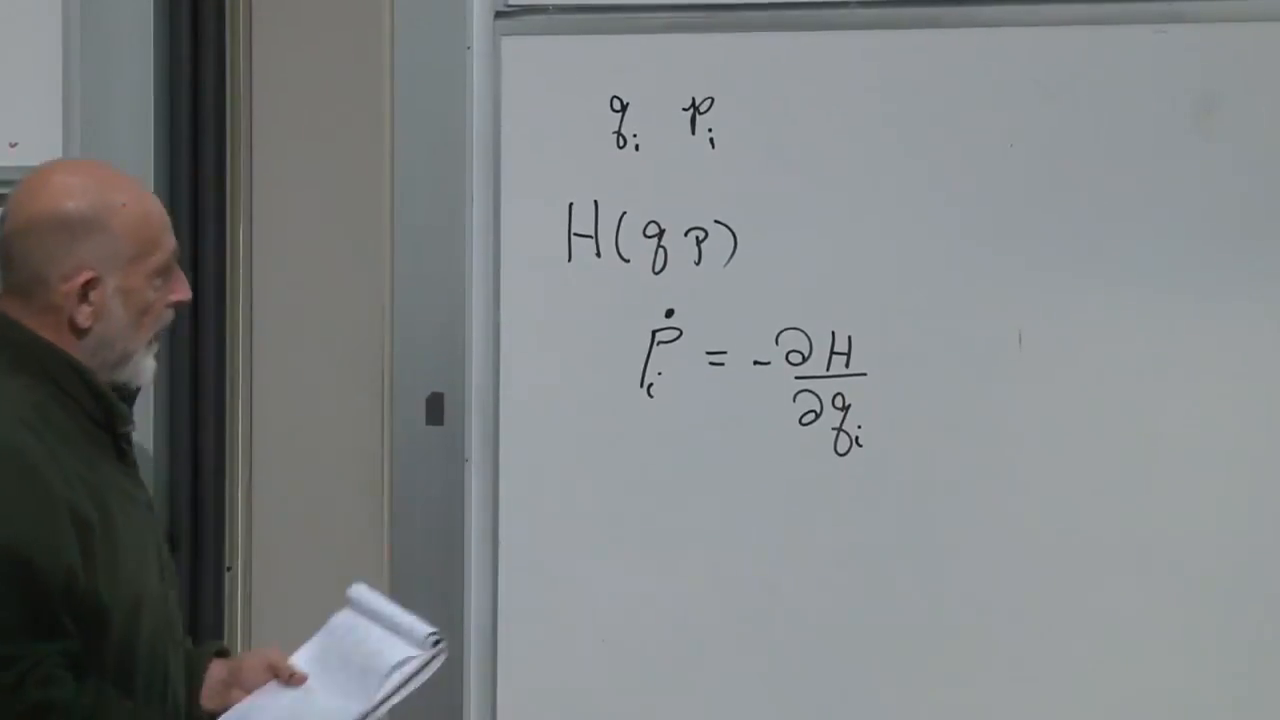
\includegraphics[width=0.82\textwidth]{lecture_07_figure_02.png}
  \caption{Канонические переменные, функция \(H(q,p)\) и гамильтоново уравнение для импульса в начале повторения.}
  \lectureframe{00:07:29}
\end{figure}

Хотя уравнения образуют пары с индексами, динамика вовсе не обязана разделяться по отдельным парам. Гамильтониан может связывать все \(q_i\) и \(p_i\), так что, например, \(\dot p_1\) может зависеть от состояния всей системы.

\begin{classroomqa}
  \audiencequestion{Является ли это изложение теперь аксиоматическим? Какое соотношение между \(p\) и \(q\) было предположено?
  \lecturetimestamp{00:17:08--00:18:18}}
  \lecturerresponse{Уравнения Гамильтона определяют формальную теорию, как только заданы \(H(q,p)\) и канонические пары. Никакого универсального дополнительного предположения \(p=m\dot q\) нет. Это соотношение выполняется для обычной частицы в декартовых координатах с квадратичной кинетической энергией, но другие координаты и другие гамильтонианы дают другие импульс--скоростные соотношения. Сами уравнения задают это соотношение через
  \(\dot q_i=\partial H/\partial p_i\). Реализуется ли предлагаемый гамильтониан в природе — отдельный физический вопрос.}
\end{classroomqa}

Теперь мы можем восстановить сохранение энергии одним рассуждением. Вдоль траектории полная производная \(H\) равна
\begin{equation}
  \frac{dH}{dt}
  =
  \sum_i\left(
    \frac{\partial H}{\partial q_i}\dot q_i
    +\frac{\partial H}{\partial p_i}\dot p_i
  \right)
  +\frac{\partial H}{\partial t}.
  \label{eq:l7-total-h-derivative}
\end{equation}
Последний член означает явную зависимость от времени при фиксированных \(q\) и \(p\), возможно потому, что меняется внешне заданный параметр. Подставляя уравнение~\eqref{eq:l7-hamilton-equations},
\begin{align}
  \frac{dH}{dt}
  &=
  \sum_i\left[
    \frac{\partial H}{\partial q_i}
    \frac{\partial H}{\partial p_i}
    -\frac{\partial H}{\partial p_i}
    \frac{\partial H}{\partial q_i}
  \right]
  +\frac{\partial H}{\partial t}\\
  &=\frac{\partial H}{\partial t}.
  \label{eq:l7-h-energy-rate}
\end{align}
Каждый член в сумме сокращается со своим парным членом. Следовательно,
\begin{equation}
  \frac{\partial H}{\partial t}=0
  \quad\Longrightarrow\quad
  \frac{dH}{dt}=0.
  \label{eq:l7-energy-conservation}
\end{equation}
Для замкнутой системы, инвариантной относительно сдвигов по времени, гамильтониан сохраняется и является энергией.

\begin{classroomqa}
  \audiencequestion{Что меняется, если гамильтониан явно зависит от времени?
  \lecturetimestamp{00:10:32--00:12:33}}
  \lecturerresponse{Тогда уравнение~\eqref{eq:l7-h-energy-rate} по-прежнему выполняется, но энергия подсистемы не обязана быть постоянной. Явная зависимость от времени обычно представляет неучтенный внешний привод, обменивающийся энергией с системой. Если этот привод включить как динамическую часть более крупной замкнутой системы, больший гамильтониан снова может не зависеть от времени явно, и его полная энергия сохраняется.}
\end{classroomqa}

\section{Энергия как геометрия в фазовом пространстве}

Предположим теперь, что \(H\) не имеет явной зависимости от времени. Начальное условие фиксирует число \(E\), и фазовая точка остается на
\begin{equation}
  H(q,p)=E.
  \label{eq:l7-energy-surface}
\end{equation}
Фазовое пространство имеет \(2n\) измерений. В регулярных точках одно уравнение на его координаты задает \((2n-1)\)-мерную гиперповерхность. Разные значения \(E\) дают разные гиперповерхности. Они не обязаны быть замкнутыми или компактными; сохранение энергии утверждает лишь, что траектория, начинающаяся на одной из них, никогда ее не покидает.

Для приведенного гармонического осциллятора из предыдущей лекции,
\begin{equation}
  H=\frac{\omega}{2}(p^2+q^2).
  \label{eq:l7-oscillator-hamiltonian}
\end{equation}
Следовательно, каждое множество постоянной энергии есть окружность,
\begin{equation}
  p^2+q^2=\frac{2E}{\omega}.
  \label{eq:l7-oscillator-circle}
\end{equation}

\begin{figure}[htbp]
  \centering
  \includegraphics[width=0.84\textwidth]{lecture_07_figure_04.png}
  \caption{Схема \(2n\)-мерного фазового пространства и гамильтониан гармонического осциллятора, используемые для введения поверхностей постоянной энергии.}
  \lectureframe{00:15:20}
\end{figure}

Уравнения движения,
\begin{equation}
  \dot q=\omega p,\qquad \dot p=-\omega q,
  \label{eq:l7-oscillator-flow}
\end{equation}
задают движение точки по часовой стрелке вдоль своей окружности. Уравнение энергии говорит, какая кривая содержит движение; уравнения Гамильтона задают направление и скорость вдоль этой кривой.

\begin{figure}[htbp]
  \centering
  \begin{tikzpicture}[scale=0.95]
    \draw[->] (-2.7,0) -- (2.7,0) node[right] {\(q\)};
    \draw[->] (0,-2.7) -- (0,2.7) node[above] {\(p\)};
    \draw[thick] (0,0) circle (0.8);
    \draw[thick] (0,0) circle (1.5);
    \draw[thick] (0,0) circle (2.2);
    \draw[->,very thick] (0,2.2) arc[start angle=90,end angle=40,radius=2.2];
    \draw[->,very thick] (1.5,0) arc[start angle=0,end angle=-50,radius=1.5];
    \draw[->,very thick] (0,-0.8) arc[start angle=-90,end angle=-140,radius=0.8];
  \end{tikzpicture}
  \caption{Постоянная энергия задает окружности; уравнения осциллятора задают касательный поток по часовой стрелке.}
\end{figure}

\begin{classroomqa}
  \audiencequestion{Являются ли два уравнения Гамильтона и \(H=E\) несколькими версиями одного и того же уравнения?
  \lecturetimestamp{00:15:53--00:17:06}}
  \lecturerresponse{Нет. Уравнения Гамильтона — это два закона движения первого порядка для одной канонической пары. Они влекут \(dH/dt=0\), из которого следует \(H=E\). Значение \(E\) выбирается начальным условием. Уравнение \(H=E\) задает поверхность; само по себе оно не определяет скорость вдоль этой поверхности.}
\end{classroomqa}

\section{От одного состояния к потоку состояний}

Вместо того чтобы следить за одним начальным условием, рассыпьте по фазовому пространству все возможные начальные условия и запустите часы. Каждая точка — это полное возможное состояние, и каждое состояние движется согласно уравнениям Гамильтона. Это рассеяние можно вообразить как пыль или как воображаемую жидкость. Ничего материального в фазовое пространство не наливают; жидкость — это способ увидеть все траектории сразу.

Поле скоростей в фазовом пространстве имеет вид
\begin{equation}
  \mathbf V(q,p,t)
  =
  (\dot q_1,\ldots,\dot q_n,\dot p_1,\ldots,\dot p_n).
  \label{eq:l7-phase-velocity}
\end{equation}
Для одной канонической пары пишем
\begin{equation}
  V_q=\dot q=\frac{\partial H}{\partial p},
  \qquad
  V_p=\dot p=-\frac{\partial H}{\partial q}.
  \label{eq:l7-phase-components}
\end{equation}
В каждой точке гамильтониан задает вектор, указывающий фазовой точке, куда идти дальше. Если \(H\) не зависит от времени, векторное поле стационарно: возвращение в ту же фазовую точку дает ту же скорость. Если \(H\) зависит от времени, само векторное поле меняется со временем, но в каждый момент оно все равно определено.

\begin{figure}[htbp]
  \centering
  \includegraphics[width=0.84\textwidth]{lecture_07_figure_05.png}
  \caption{Поле скоростей гармонического осциллятора. Векторы касательны к окружностям и укорачиваются по мере приближения к началу координат.}
  \lectureframe{00:24:50}
\end{figure}

Для гармонического осциллятора каждый радиус-вектор вращается с угловой скоростью \(\omega\). Точки вблизи начала координат имеют меньшую линейную скорость, потому что за тот же период проходят окружность меньшей длины. Поэтому вся пыль вращается как жесткая карусель.

\begin{classroomqa}
  \audiencequestion{Означает ли жесткое вращение, что все траектории осциллятора имеют один и тот же период? \lecturetimestamp{00:21:10--00:21:42}}
  \lecturerresponse{Да. Именно эта независимость от амплитуды и есть определяющее особое свойство гармонического осциллятора. Каждая окружность обходится с одной и той же угловой частотой \(\omega\), хотя модуль скорости в фазовом пространстве на меньшей окружности меньше.}
\end{classroomqa}

\begin{classroomqa}
  \audiencequestion{Одинаков ли вектор скорости в фазовом пространстве в каждой точке?
  \lecturetimestamp{00:24:29--00:25:37}}
  \lecturerresponse{Нет. И его направление, и его модуль в общем случае зависят от положения. Для осциллятора этот вектор касается локальной окружности и имеет модуль \(\omega\sqrt{p^2+q^2}\). Векторное поле означает, что каждой точке поставлен в соответствие один вектор, а не что повсюду скопирован один и тот же вектор.}
\end{classroomqa}

\begin{classroomqa}
  \audiencequestion{Что именно здесь играет роль частиц и плотности этой воображаемой жидкости? \lecturetimestamp{00:56:03--00:58:40}}
  \lecturerresponse{Каждая точка — это одно полное состояние всей механической системы. Это не отдельная физическая частица. Для пяти частиц, движущихся в одном пространственном измерении, нужны пять координат и пять импульсов, следовательно, фазовое пространство 10-мерно; в трех измерениях требуется 30 измерений. Эта пыль есть ансамбль альтернативных состояний. Если образ жидкости отвлекает, просто возьмите область начальных условий, проследите эволюцию каждой точки в ней и сравните ее объем в фазовом пространстве до и после.}
\end{classroomqa}

\section{Сжатие и дивергенция}

Чтобы выяснить, теряет ли эта воображаемая жидкость объем, начнем с одного измерения.
Пусть точки на прямой движутся со скоростью \(v(x)\). Для двух близких точек, разделенных расстоянием \(\delta x\), разность скоростей равна
\begin{equation}
  \delta v \simeq \frac{dv}{dx}\,\delta x.
  \label{eq:l7-one-dimensional-strain}
\end{equation}
Если \(dv/dx>0\), передняя точка движется быстрее, и интервал растягивается. Если
\(dv/dx<0\), он сжимается. Стационарное одномерное несжимаемое течение,
следовательно, удовлетворяет
\begin{equation}
  \frac{dv}{dx}=0.
  \label{eq:l7-one-dimensional-incompressible}
\end{equation}

\begin{figure}[htbp]
  \centering
  \includegraphics[width=0.84\textwidth]{lecture_07_figure_06.png}
  \caption{Одномерная конструкция, приводящая к \(dv/dx\) как к локальной скорости растяжения или сжатия.}
  \lectureframe{00:30:20}
\end{figure}

Есть две эквивалентные точки зрения. Мы можем следить за материальным отрезком и спрашивать, меняется ли его длина. Или можем удерживать малый отрезок фиксированным и спрашивать, равно ли количество, входящее за единицу времени, количеству, выходящему.
В первом случае мы следуем за жидкостью; во втором наблюдаем, как она проходит мимо.

В размерности больше единицы область может растягиваться вдоль одной оси и сжиматься вдоль другой, не меняя полного объема. Для поля скоростей
\(\mathbf V=(V_x,V_y,V_z)\), соответствующей локальной величиной является дивергенция,
\begin{equation}
  \nabla\cdot\mathbf V
  =
  \frac{\partial V_x}{\partial x}
  +\frac{\partial V_y}{\partial y}
  +\frac{\partial V_z}{\partial z}.
  \label{eq:l7-spatial-divergence}
\end{equation}
Положительная дивергенция означает локальное расширение, отрицательная — локальное
сжатие, а несжимаемость выражается условием
\begin{equation}
  \nabla\cdot\mathbf V=0.
  \label{eq:l7-zero-divergence}
\end{equation}
Равенство притока и оттока через фиксированный малый ящик — это то же локальное утверждение,
что и сохранение объема малого ящика, движущегося вместе с потоком.

\begin{figure}[htbp]
  \centering
  \includegraphics[width=0.86\textwidth]{lecture_07_figure_07.png}
  \caption{Двумерный ящик, его компоненты потока и сумма производных по соответствующим координатам, определяющая дивергенцию.}
  \lectureframe{00:35:30}
\end{figure}

\begin{classroomqa}
  \audiencequestion{Идет ли речь о жидкости в обычном пространстве или о потоке в
  фазовом пространстве? \lecturetimestamp{00:34:27--00:34:40}}
  \lecturerresponse{Сначала это просто общее рассуждение о жидкости.
  Мы применим его к фазовому пространству четной размерности, где координатными
  направлениями являются \(q_i\) и \(p_i\), а компонентами скорости —
  \(\dot q_i\) и \(\dot p_i\).}
\end{classroomqa}

Теперь вернемся к дискретным отображениям состояний. В обратимом цикле в каждый узел
входит одна стрелка и из него выходит одна стрелка, и выбранное множество состояний сохраняет
то же число элементов по мере эволюции. В стоке входит много стрелок, а выходит слишком мало;
несколько альтернатив становятся неразличимыми.

\begin{figure}[htbp]
  \centering
  \includegraphics[width=0.80\textwidth]{lecture_07_figure_08.png}
  \caption{Дискретный сток, используемый, чтобы вновь связать дивергенцию с
  критерием обратимых законов из первой лекции.}
  \lectureframe{00:40:15}
\end{figure}

Теперь в непрерывном случае вопрос ставится точно: имеет ли гамильтонов поток нулевую
дивергенцию, так что малая область различимых состояний никогда не сплющивается в меньший
объем фазового пространства?

\section{Теорема Лиувилля}

\begin{theorem}[Liouville's theorem]
Для гладкой гамильтоновой системы каноническое поле скоростей в фазовом пространстве имеет
нулевую дивергенцию:
\begin{equation}
  \sum_i\left(
    \frac{\partial\dot q_i}{\partial q_i}
    +\frac{\partial\dot p_i}{\partial p_i}
  \right)=0.
  \label{eq:l7-liouville-divergence}
\end{equation}
Эквивалентно, гамильтонова эволюция сохраняет канонический фазовый объем
\(dq_1\cdots dq_n\,dp_1\cdots dp_n\).
\end{theorem}

\begin{classroomqa}
  \audiencequestion{Компоненты, обозначенные \(V\), — это просто производные по времени от \(p\) и
  \(q\)? \lecturetimestamp{00:42:20--00:43:22}}
  \lecturerresponse{Да. Для одной пары
  \(V_q=\dot q\) и \(V_p=\dot p\). Если выписать все такие производные в ряд, получится
  вектор скорости потока во всем фазовом пространстве.}
\end{classroomqa}

Для одной канонической пары уравнения Гамильтона дают
\begin{equation}
  V_p=-\frac{\partial H}{\partial q},
  \qquad
  V_q=\frac{\partial H}{\partial p}.
  \label{eq:l7-liouville-components}
\end{equation}
Поэтому дивергенция равна
\begin{align}
  \frac{\partial V_p}{\partial p}
  +\frac{\partial V_q}{\partial q}
  &=
  -\frac{\partial}{\partial p}
    \left(\frac{\partial H}{\partial q}\right)
  +\frac{\partial}{\partial q}
    \left(\frac{\partial H}{\partial p}\right)\\
  &=
  -\frac{\partial^2H}{\partial p\,\partial q}
  +\frac{\partial^2H}{\partial q\,\partial p}
  =0.
  \label{eq:l7-liouville-proof}
\end{align}

\begin{figure}[htbp]
  \centering
  \includegraphics[width=0.86\textwidth]{lecture_07_figure_09.png}
  \caption{Прямоугольник конечных разностей, используемый для объяснения того, почему гладкие смешанные
  частные производные перестановочны.}
  \lectureframe{00:47:30}
\end{figure}

Равенство смешанных частных производных можно увидеть, если рассмотреть четыре близкие точки
\(A,B,C,D\) в вершинах малого прямоугольника в плоскости \(q\)-\(p\).
Сначала взяв разность по \(q\), а затем по \(p\), мы получаем, с точностью до множителя из двух
малых длин сторон,
\begin{equation}
  F(B)+F(D)-F(A)-F(C).
  \label{eq:l7-finite-difference-combination}
\end{equation}
Если брать разности в обратном порядке, получается та же комбинация.
В пределе малого прямоугольника это дает
\(\partial_p\partial_qF=\partial_q\partial_pF\), при условии непрерывности требуемых
производных.

\begin{figure}[htbp]
  \centering
  \includegraphics[width=0.88\textwidth]{lecture_07_figure_10.png}
  \caption{Каноническая дивергенция после того, как уравнения Гамильтона свели
  ее к двум смешанным производным с противоположными знаками.}
  \lectureframe{00:50:20}
\end{figure}

Для многих степеней свободы то же сокращение происходит для каждой канонической
пары:
\begin{align}
  \sum_i\left(
    \frac{\partial\dot p_i}{\partial p_i}
    +\frac{\partial\dot q_i}{\partial q_i}
  \right)
  &=
  \sum_i\left(
    -\frac{\partial^2H}{\partial p_i\,\partial q_i}
    +\frac{\partial^2H}{\partial q_i\,\partial p_i}
  \right)\\
  &=0.
  \label{eq:l7-many-pair-proof}
\end{align}
Растяжение вдоль одного канонического направления уравновешивается сжатием в его
сопряженном направлении. Такое попарное сокращение выражает более сильную структуру, чем
случайная компенсация между несвязанными осями.

\begin{classroomqa}
  \audiencequestion{Подразумевается ли суммирование по всем каноническим парам?
  \lecturetimestamp{00:52:00--00:52:36}}
  \lecturerresponse{Да. В формуле~\eqref{eq:l7-many-pair-proof} суммирование ведется по
  \(i\), и две смешанные производные сокращаются отдельно внутри каждой
  пары \(q_i,p_i\).}
\end{classroomqa}

\begin{classroomqa}
  \audiencequestion{Выписанная дивергенция выглядит декартовой. Сохраняется ли
  теорема при замене координат?
  \lecturetimestamp{00:52:50--00:53:22,\allowbreak\ 00:58:18--00:58:40}}
  \lecturerresponse{Естественная формулировка дается в канонических координатах
  и с каноническим элементом объема
  \(dq_1\cdots dq_n\,dp_1\cdots dp_n\). Каноническое, или симплектическое,
  преобразование совместно изменяет координаты и импульсы и сохраняет этот
  объем. В произвольных неканонических координатах в мере объема должен
  присутствовать якобиан; наивное произведение приращений координат не обязано
  быть инвариантным.}
\end{classroomqa}

\begin{classroomqa}
  \audiencequestion{Требует ли теорема Лиувилля гамильтониана, не зависящего от
  времени? \lecturetimestamp{00:53:43--00:55:51}}
  \lecturerresponse{Нет. Сохранение энергии требовало
  \(\partial H/\partial t=0\), но доказательство для дивергенции дифференцирует только
  по \(q_i\) и \(p_i\) при фиксированном времени. Смешанные частные производные по-прежнему
  сокращаются для \(H(q,p,t)\). Следовательно, зависящий от времени гамильтониан
  порождает зависящий от времени, но в каждый данный момент сохраняющий объем
  канонический поток.}
\end{classroomqa}

\section{Что означает и чего не означает сохранение объема}

Возьмите любую малую область \(R_0\) начальных условий и проследите эволюцию каждой точки в течение
времени \(t\). Теорема Лиувилля утверждает
\begin{equation}
  \operatorname{Vol}(R_t)=\operatorname{Vol}(R_0).
  \label{eq:l7-volume-preservation}
\end{equation}
Область может перемещаться, вращаться, деформироваться сдвигом и вытягиваться в длинную нить. Ее
объем, а не форма, сохраняется. Различные фазовые точки не могут сливаться при
конечной гладкой гамильтоновой эволюции.

Для конечных времен гладкий гамильтонов поток представляет собой обратимое отображение с гладким
обратным отображением, получаемым эволюцией назад по времени. Это также объясняет прозвучавшее
на лекции утверждение, что связная область не может перетянуться и распасться на несвязанные части:
поток непрерывно деформирует область и сохраняет ее топологию, хотя чрезвычайно тонкая перемычка
может при конечном разрешении создать видимость, что две доли разделены.

\begin{figure}[htbp]
  \centering
  \includegraphics[width=0.86\textwidth]{lecture_07_figure_12.png}
  \caption{Возможные деформации одной области фазового пространства. Гладкий
  гамильтонов поток может образовать тонкую перемычку, но не подлинный разрыв за конечное время
  на части, эволюционирующие независимо.}
  \lectureframe{01:04:55}
\end{figure}

\begin{classroomqa}
  \audiencequestion{Может ли область фазового пространства перетянуться и разделиться на две
  части? \lecturetimestamp{01:04:10--01:05:49}}
  \lecturerresponse{Не при гладком детерминистическом гамильтоновом потоке за
  конечное время. В гипотетической точке пережатия по-прежнему есть одна точка фазового пространства
  и одна приписанная ей скорость, а не два несовместимых направления. Область
  может образовать очень длинную узкую соединяющую нить, но
  эволюция остается взаимно однозначной и не разрывает ее.}
\end{classroomqa}

\begin{classroomqa}
\audiencequestion{Являются ли две далеко разошедшиеся части растянутого пятна физически связанными или квантово запутанными?
\lecturetimestamp{01:08:01--01:09:16}}
\lecturerresponse{Никакая такая физическая связь не подразумевается. Это пятно — набор альтернативных начальных условий, а не один материальный объект. Называя его одной областью, мы лишь фиксируем общее множество, из которого эволюционировали эти состояния; это ничего не говорит ни о силах между ними, ни о квантовой запутанности.
}
\end{classroomqa}

\begin{classroomqa}
\audiencequestion{Что происходит вблизи верхнего неустойчивого равновесия жёсткого маятника? Перекрываются ли траектории, идущие по часовой стрелке и против неё?
\lecturetimestamp{01:07:07--01:07:47}}
\lecturerresponse{Близкие начальные условия могут разойтись по очень разным траекториям, образуя только что описанные тонкие нити. Они не становятся одной и той же точкой фазового пространства: две стороны различаются знаком бесконечно малого смещения или импульса. Состояние точного баланса имеет собственное однозначно определённое движение, а именно в идеальной модели остаётся в равновесии.}
\end{classroomqa}

\subsection{Растяжение в пространстве координат и сжатие в пространстве импульсов}

Если каноническое преобразование растягивает некоторый диапазон координат в \(a\) раз,
то масштаб сопряжённого импульса сжимается в обратное число раз:
\begin{equation}
  q\longrightarrow aq,
  \qquad
  p\longrightarrow \frac{p}{a},
  \qquad
  dq\,dp\longrightarrow dq\,dp.
  \label{eq:l7-canonical-scaling}
\end{equation}
В этом состоит ясное фазово-пространственное содержание примера с расширением газа. При адиабатическом расширении доступная область обычного пространства увеличивается, тогда как типичные импульсы уменьшаются и газ охлаждается. Конкретное термодинамическое соотношение зависит от размерности, протокола расширения и взаимодействий; теорема Лиувилля задаёт ограничение на объём, а не каждый термодинамический коэффициент.

\begin{classroomqa}
\audiencequestion{Применимо ли то же рассуждение к расширяющейся Вселенной, даже при внезапном расширении? \lecturetimestamp{00:53:23--00:56:00}}
\lecturerresponse{Теорема Лиувилля применима всякий раз, когда полная динамика является гамильтоновой, включая случай явно зависящих от времени канонических переменных. Расширение по координатным направлениям должно сопровождаться соответствующим сжатием по направлениям канонических импульсов. Однако космологический масштабный фактор, управляемое расширение газа и свободно разлетающееся облако — не один и тот же физический процесс. Хабблоподобная корреляция между расстоянием и скоростью удаления может возникать потому, что более быстрые объекты улетают дальше, тогда как адиабатическое охлаждение связано со сжатием локального распределения импульсов. В обоих случаях теорема накладывает ограничение на полное отображение фазового пространства.}
\end{classroomqa}

\begin{classroomqa}
\audiencequestion{Какое практическое применение имеет теорема Лиувилля?
\lecturetimestamp{01:06:16--01:07:04}}
\lecturerresponse{Она занимает центральное место в статистической механике. Она определяет, как эволюционируют ансамбли микроскопических состояний, и лежит в основе связи между объёмом фазового пространства и энтропией. Расширение и охлаждение газа — одна непосредственная иллюстрация; далее она становится базовым инструментом для рассуждений о равновесных и неравновесных системах.}
\end{classroomqa}

\section{Поток, резко меняющий форму}

Гармонический осциллятор сохраняет и площадь, и форму, потому что его поток представляет собой жёсткое вращение. Это исключительный случай. Чтобы отделить сохранение объёма от жёсткости, рассмотрим
\begin{equation}
  H=\lambda pq,
  \label{eq:l7-pq-hamiltonian}
\end{equation}
где \(\lambda\) имеет размерность обратного времени. В лекции полагается
\(\lambda=1\); сохраняя этот параметр, мы явно видим размерности.

\begin{figure}[htbp]
\centering
  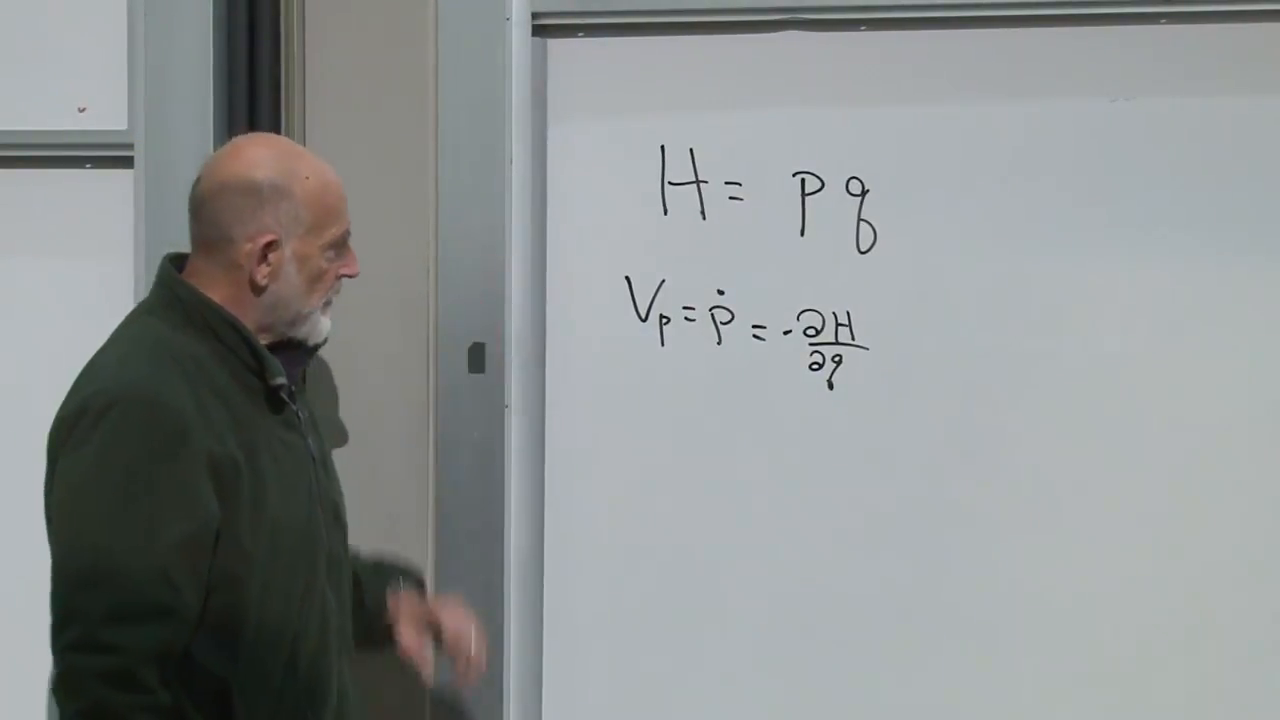
\includegraphics[width=0.82\textwidth]{lecture_07_figure_03.png}
\caption{Начало примера с \(H=pq\) и первая компонента фазовой скорости.}
\lectureframe{01:00:11}
\end{figure}

Уравнения Гамильтона имеют вид
\begin{equation}
  \dot p=-\lambda p,
  \qquad
  \dot q=\lambda q,
  \label{eq:l7-pq-flow}
\end{equation}
с решениями
\begin{equation}
  p(t)=p_0e^{-\lambda t},
  \qquad
  q(t)=q_0e^{\lambda t}.
  \label{eq:l7-pq-solutions}
\end{equation}
Квадратный участок экспоненциально сжимается по \(p\) и растягивается на тот же множитель по \(q\):
\begin{equation}
  \Delta p(t)\Delta q(t)
  =
  \Delta p(0)\Delta q(0).
  \label{eq:l7-pq-area}
\end{equation}
Дивергенция потока локально подтверждает этот результат,
\begin{equation}
  \frac{\partial\dot p}{\partial p}
  +\frac{\partial\dot q}{\partial q}
  =-\lambda+\lambda=0.
  \label{eq:l7-pq-divergence}
\end{equation}

\begin{figure}[htbp]
\centering
  \includegraphics[width=0.86\textwidth]{lecture_07_figure_11.png}
\caption{Компактный участок, растянутый в длинную тонкую полосу при сохранении площади в потоке \(H=pq\).}
\lectureframe{01:02:10}
\end{figure}

\begin{classroomqa}
\audiencequestion{Поскольку \(pq\) имеет размерность действия, является ли теорема Лиувилля законом сохранения действия? \lecturetimestamp{01:03:00--01:04:09}}
\lecturerresponse{Нет. Теорема сохраняет объём фазового пространства. Для одной канонической пары \(dq\,dp\) имеет размерность действия, и этот факт размерности предвосхищает квантовую механику, где ячейки фазового пространства измеряются в единицах, задаваемых \(\hbar\). Но произведение \(pq\) само по себе не является функционалом действия Гамильтона и не становится автоматически моментом импульса лишь потому, что размерности совпадают.}
\end{classroomqa}

Этот пример также показывает, что углы не обязаны сохраняться. Прямоугольный крест с неравными компонентами при масштабировании по формуле~\eqref{eq:l7-pq-solutions} как метрическая фигура подвергается сдвиговой деформации, тогда как площадь остаётся неизменной. Теорема Лиувилля — это теорема о площади или объёме, а не обычная теорема об евклидовой жёсткости.

\section{Затухание порождает сток}

Чтобы увидеть, что именно исключает теорема, рассмотрим редуцированное уравнение для затухающего осциллятора,
\begin{equation}
  m\ddot x=-kx-c\dot x,
  \qquad c>0.
  \label{eq:l7-damped-newton}
\end{equation}
Положим \(p=m\dot x\). Тогда
\begin{equation}
  \dot x=\frac{p}{m},
  \qquad
  \dot p=-kx-\frac{c}{m}p.
  \label{eq:l7-damped-first-order}
\end{equation}
Без затухания фазовая точка обращается вокруг начала координат. При наличии затухания энергия передаётся микроскопическим степеням свободы окружающей среды, и орбита закручивается внутрь по спирали.

\begin{figure}[htbp]
\centering
  \includegraphics[width=0.84\textwidth]{lecture_07_figure_13.png}
\caption{Уравнение затухающего осциллятора и его спираль, закручивающаяся внутрь, на плоскости \(x\)-\(p\).}
\lectureframe{01:13:30}
\end{figure}

Дивергенция этого редуцированного двумерного потока равна
\begin{equation}
  \frac{\partial\dot x}{\partial x}
  +\frac{\partial\dot p}{\partial p}
  =
  0-\frac{c}{m}<0.
  \label{eq:l7-damped-divergence}
\end{equation}
Любой конечный участок сжимается. Начало координат является стоком, непрерывным аналогом диаграммы состояний, в которой многие стрелки входят в одно состояние.

\begin{figure}[htbp]
\centering
  \includegraphics[width=0.88\textwidth]{lecture_07_figure_14.png}
\caption{Компоненты фазовой скорости при затухании, использованные для получения отрицательной дивергенции \(-c/m\).}
\lectureframe{01:16:05}
\end{figure}

Это не означает, что микроскопическая механика нарушает теорему Лиувилля. Две переменные \(x,p\) не учитывают огромное число степеней свободы среды, которые принимают энергию осциллятора. Расширенная система «осциллятор плюс среда» может быть гамильтоновой и сохранять объём, хотя её редуцированное описание в переменных \(x,p\) сжимается.

\begin{classroomqa}
\audiencequestion{Описывается ли затухающий осциллятор по-прежнему уравнением Ньютона, хотя в этом редуцированном фазовом пространстве он не является гамильтоновым?
\lecturetimestamp{01:20:09--01:21:12}}
\lecturerresponse{Да. В \(F=ma\) можно включить эмпирически заданную силу сопротивления. Элементарное описание с \(L=T-V\) и гамильтонианом непосредственно применимо к консервативным силам, а более общие лагранжианы позволяют учитывать и некоторые силы, зависящие от скорости. Однако марковский член трения для изолированной пары \(x,p\) — это редуцированная диссипативная динамика, а не замкнутая каноническая гамильтонова система.}
\end{classroomqa}

\begin{classroomqa}
\audiencequestion{Если затухающие уравнения можно интегрировать назад при бесконечной точности, действительно ли информация теряется?
\lecturetimestamp{01:25:16--01:27:17}}
\lecturerresponse{Для любого конечного времени идеальное дифференциальное уравнение всё ещё имеет обратное отображение, так что точные данные можно проследить назад. Точное утверждение состоит в том, что конечные ячейки фазового пространства экспоненциально сжимаются. Поэтому восстановление их прошлого требует экспоненциально растущей точности, а при бесконечном времени все траектории приближаются к стоку. Это наиболее близкий непрерывный классический аналог дискретной картины потери альтернатив, а не утверждение, будто два точных решения при конечном времени буквально становятся одним.}
\end{classroomqa}

\begin{classroomqa}
\audiencequestion{Может ли векторное поле иметь нулевую дивергенцию, не будучи порождённым гамильтонианом? \lecturetimestamp{01:18:21--01:22:34}}
\lecturerresponse{Конечно. Гамильтонова форма достаточна для нулевой дивергенции, но не необходима. Произвольное несжимаемое поле скоростей может иметь нулевую дивергенцию, не будучи каноническим гамильтоновым полем на том же самом пространстве. Обычный учебный пример — трёхмерное несжимаемое поле скорости жидкости: три координаты сами по себе не могут образовать канонические пары. Полная механика жидкости может допускать более сложные бесконечномерные гамильтоновы формулировки, но это не отменяет одностороннего следствия, о котором здесь идёт речь.}
\end{classroomqa}

\section{Дополнительные различия, выявленные вопросами}

\begin{classroomqa}
\audiencequestion{Как связано движение по поверхности постоянной энергии с сохранением всего объёма фазового пространства?
\lecturetimestamp{01:28:47--01:30:41}}
\lecturerresponse{Это независимые следствия гамильтоновой структуры. Если \(H\) не зависит от времени, каждая траектория остаётся на своей собственной поверхности энергии. Конечный участок может пересекать много таких поверхностей; теорема Лиувилля утверждает, что объём всего этого участка сохраняется. Для гармонического осциллятора этот участок сохраняет также и форму, потому что поток представляет собой жёсткое вращение. Для \(H=pq\) он сохраняет только площадь, но не форму.}
\end{classroomqa}

\begin{classroomqa}
  \audiencequestion{Как механическая работа вписывается в гамильтоново описание?
  \lecturetimestamp{01:30:44--01:32:57}}
  \lecturerresponse{Работа описывает энергию, передаваемую через выбранную границу системы. Внешний агент может поднять груз или изменить параметр и тем самым изменить энергию подсистемы; энергия, которую он сообщает, теряется самим агентом. Если обе стороны включены в одну замкнутую модель, акцент вновь смещается на сохранение полной энергии и обмен между подсистемами.}
\end{classroomqa}

\begin{classroomqa}
  \audiencequestion{Сохраняются ли при сохранении объема также топология и углы?
  \lecturetimestamp{01:33:00--01:33:37}}
  \lecturerresponse{Гладкий гамильтонов поток за конечное время сохраняет топологию, потому что он является обратимой непрерывной деформацией. В общем случае он не сохраняет евклидовы углы или форму. Жесткое вращение осциллятора их сохраняет, но растяжение при \(H=pq\) показывает, почему это особый случай.}
\end{classroomqa}

\begin{classroomqa}
  \audiencequestion{Было ли преобразование Лежандра опущено потому, что оно не имеет физического значения?
  \lecturetimestamp{01:33:43--01:34:48}}
  \lecturerresponse{Нет. Это полезное преобразование, которое заменяет описание через скорости описанием через импульсы и дает \(H=\sum_i p_i\dot q_i-L\), когда отображение регулярно. Эта конструкция уже неоднократно использовалась, даже когда ее формальное название не подчеркивалось; подробная общая теория просто не нужна для настоящей теоремы.}
\end{classroomqa}

\section{Скобки Пуассона: следующее сжатие}

В заключительные минуты изложение возвращается к исторической теме. Механика XIX века вновь и вновь искала компактные структуры, связывающие кажущиеся различными системы --- механику и геометрическую оптику, частицы и лучи, классические траектории и волновые описания. Скобки Пуассона — еще одна такая структура, и в квантовой механике они становятся особенно важными.

Пусть \(F(q,p)\) — любая функция на фазовом пространстве. Это может быть координата, импульс, произведение \(qp\) или момент импульса. В ходе движения имеем
\begin{equation}
  \frac{dF}{dt}
  =
  \sum_i\left(
    \frac{\partial F}{\partial q_i}\dot q_i
    +\frac{\partial F}{\partial p_i}\dot p_i
  \right).
  \label{eq:l7-f-time-derivative}
\end{equation}
Подставляя уравнения Гамильтона, получаем:
\begin{equation}
  \frac{dF}{dt}
  =
  \sum_i\left(
    \frac{\partial F}{\partial q_i}
    \frac{\partial H}{\partial p_i}
    -
    \frac{\partial F}{\partial p_i}
    \frac{\partial H}{\partial q_i}
  \right).
  \label{eq:l7-f-hamiltonian-derivative}
\end{equation}

\begin{figure}[htbp]
  \centering
  \includegraphics[width=0.88\textwidth]{lecture_07_figure_15.png}
  \caption{Правило цепочки для производной по времени от произвольной функции фазового пространства \(F(q,p)\).}
  \lectureframe{01:42:40}
\end{figure}

Повторяющаяся антисимметричная комбинация заслуживает названия. Для любых двух функций \(F\) и \(G\) определим их скобку Пуассона равенством
\begin{equation}
  \boxed{
  \{F,G\}
  =
  \sum_i\left(
    \frac{\partial F}{\partial q_i}
    \frac{\partial G}{\partial p_i}
    -
    \frac{\partial F}{\partial p_i}
    \frac{\partial G}{\partial q_i}
  \right).}
  \label{eq:l7-poisson-bracket}
\end{equation}

\begin{figure}[htbp]
  \centering
  \includegraphics[width=0.86\textwidth]{lecture_07_figure_16.png}
  \caption{Комбинация производных двух функций, получающая статус скобки Пуассона.}
  \lectureframe{01:44:15}
\end{figure}

Уравнение~\eqref{eq:l7-f-hamiltonian-derivative} принимает вид
\begin{equation}
  \boxed{\frac{dF}{dt}=\{F,H\}.}
  \label{eq:l7-hamiltonian-poisson-evolution}
\end{equation}
Если \(F\) также явно зависит от времени, следует добавить \(\partial F/\partial t\). При выборе \(F=q_i\) или \(F=p_i\) получаются два уравнения Гамильтона, так что уравнение~\eqref{eq:l7-hamiltonian-poisson-evolution} представляет собой компактную форму полной динамики.

Запись всегда можно искусственно сжать --- можно было бы возвести много уравнений в квадрат, сложить их и назвать результат одним уравнением. Это скорее скрывало бы структуру, чем выявляло ее. Скобка Пуассона полезна по противоположной причине: ее алгебра организует временную эволюцию, сохраняющиеся величины и симметрию. Следующий шаг — развить эту алгебру, а затем применить ее к моменту импульса, структура которого будет центральной и в классической механике, и в квантовой теории.

\section{Непрерывный смысл обратимости}

Теперь мы можем изложить эту цепочку идей, не сокращая ее. Уравнения Гамильтона сохраняют \(H\), когда гамильтониан не имеет явной зависимости от времени, так что отдельные траектории остаются на гиперповерхностях постоянной энергии. Те же уравнения задают скорость каждой точке фазового пространства. Дивергенция этой скорости обращается в нуль, поскольку смешанные частные производные попарно сокращаются. Следовательно, целая область возможных состояний сохраняет свой канонический объем.

Это непрерывная версия одной входящей и одной выходящей стрелки. Форма может изменяться, углы могут изменяться, и соседние траектории могут расходиться чрезвычайно сильно. Чего не может произойти в гладком замкнутом гамильтоновом описании, так это сжатия конечного набора альтернатив в меньший объем фазового пространства. Поток при \(H=pq\) демонстрирует возможность растяжения; редуцированный затухающий осциллятор демонстрирует сток, который появляется, как только от гамильтоновых условий отказываются. Скобки Пуассона затем сводят ту же динамику к утверждению, что гамильтониан порождает любую производную по времени.

\chapter{Скобки Пуассона, генераторы и момент импульса}

\lectureoverview{Скобка Пуассона — это не просто компактный способ переписать уравнения Гамильтона. Это алгебраическая операция, порождающая преобразования. Скобка с гамильтонианом порождает эволюцию во времени; скобка с импульсом порождает трансляции; скобка с моментом импульса порождает вращения. На этом языке симметрия и закон сохранения становятся двумя прочтениями одного и того же равенства скобки нулю. Мы разовьём эту идею, начиная с гармонического осциллятора, а затем используем алгебру момента импульса, чтобы получить гироскопическую прецессию без введения углов Эйлера.}

\section{Функция вдоль гамильтоновой траектории}

Пусть
\[
  F=F(q_1,\ldots,q_n,p_1,\ldots,p_n)
\]
— достаточно гладкая функция на фазовом пространстве. Её можно рассматривать двояко. Во-первых, она ставит в соответствие число каждой точке фазового пространства. Во-вторых, после выбора гамильтоновой траектории она становится функцией времени, поскольку точка \((q(t),p(t))\) движется. Вдоль этой траектории
\begin{equation}
  \frac{dF}{dt}
  =
  \sum_i\left(
    \frac{\partial F}{\partial q_i}\dot q_i
    +\frac{\partial F}{\partial p_i}\dot p_i
  \right).
  \label{eq:l8-chain-rule}
\end{equation}
а уравнения Гамильтона,
\begin{equation}
  \dot q_i=\frac{\partial H}{\partial p_i},
  \qquad
  \dot p_i=-\frac{\partial H}{\partial q_i},
  \label{eq:l8-hamilton-equations}
\end{equation}
превращают это в
\begin{equation}
  \frac{dF}{dt}
  =
  \sum_i\left(
    \frac{\partial F}{\partial q_i}
    \frac{\partial H}{\partial p_i}
    -
    \frac{\partial F}{\partial p_i}
    \frac{\partial H}{\partial q_i}
  \right).
  \label{eq:l8-fdot-expanded}
\end{equation}
Комбинация в правой части встречается повсюду в классической механике, даже когда ни один из её аргументов не является гамильтонианом. Это мотивирует определение
\begin{equation}
  \boxed{
  \{F,G\}
  =
  \sum_i\left(
    \frac{\partial F}{\partial q_i}
    \frac{\partial G}{\partial p_i}
    -
    \frac{\partial F}{\partial p_i}
    \frac{\partial G}{\partial q_i}
  \right).}
  \label{eq:l8-poisson-definition}
\end{equation}
Поэтому уравнение~\eqref{eq:l8-fdot-expanded} принимает вид
\begin{equation}
  \boxed{\dot F=\{F,H\}.}
  \label{eq:l8-time-generator}
\end{equation}

\begin{classroomqa}
  \audiencequestion{Если второй аргумент заменить \(H\) на произвольную функцию \(G\), будет ли скобка по-прежнему производной \(F\) по времени?
  \lecturetimestamp{00:05:45--00:06:15}}
  \lecturerresponse{Нет. По мере обобщения обозначений аудитория улавливает важный момент. Уравнение~\eqref{eq:l8-poisson-definition}
  определяет \(\{F,G\}\) для любых двух функций на фазовом пространстве, но
  \(\dot F=\{F,G\}\) верно только тогда, когда \(G\) — гамильтониан. Произвольное
  \(G\) будет порождать другое бесконечно малое преобразование.}
\end{classroomqa}

Полезно записывать малое изменение во времени в виде
\begin{equation}
  \delta_t F=\epsilon\,\{F,H\}.
  \label{eq:l8-small-time-step}
\end{equation}
Эта форма предвосхищает то, что появится дальше. Эволюция во времени — лишь один представитель более широкого семейства преобразований, порождаемых скобками Пуассона.

\section{Алгебра скобок}

Теперь скобку можно использовать как самостоятельное исчисление. Её правила следуют из обычного дифференцирования:
\begin{align}
  \{A,B\}&=-\{B,A\}, \label{eq:l8-antisymmetry}\\
  \{A+B,C\}&=\{A,C\}+\{B,C\}, \label{eq:l8-additivity}\\
  \{\lambda A,B\}&=\lambda\{A,B\},
    \quad \lambda\ \text{constant}, \label{eq:l8-scalar-rule}\\
  \{AB,C\}&=A\{B,C\}+\{A,C\}B. \label{eq:l8-leibniz}
\end{align}
Эти четыре строки выражают соответственно антисимметрию, аддитивность, линейность при умножении на константу и правило Лейбница.
Классические функции на фазовом пространстве перемножаются коммутативно, поэтому расположение обычных множителей \(A\) и \(B\) в последней строке несущественно. Для операторов в квантовой механике это уже неверно. Антисимметрия также влечёт
\begin{equation}
  \{A,A\}=0.
  \label{eq:l8-self-bracket}
\end{equation}

Для канонических координат элементарные скобки имеют вид
\begin{equation}
  \boxed{
  \{q_i,q_j\}=0,\qquad
  \{p_i,p_j\}=0,\qquad
  \{q_i,p_j\}=\delta_{ij}.}
  \label{eq:l8-canonical-brackets}
\end{equation}
Любая функция только от \(q_i\) имеет нулевую скобку с любой другой функцией только от \(q_i\); аналогичное утверждение верно для функций только от \(p_i\). Чтобы скобка была ненулевой, каноническая координата должна встретиться со своим сопряжённым импульсом. Дельта Кронекера в ур.~\eqref{eq:l8-canonical-brackets} показывает, что встречаются только совпадающие индексы.

\subsection{Гармонический осциллятор как проверка}

Рассмотрим
\begin{equation}
  H=\frac{p^2}{2m}+\frac{kq^2}{2}.
  \label{eq:l8-oscillator-hamiltonian}
\end{equation}
Теперь мы намеренно используем только правила для скобок и
Eq.~\eqref{eq:l8-time-generator}. Сначала
\begin{align}
  \dot q
  &=\{q,H\}\\
  &=\frac{1}{2m}\{q,p^2\}\\
  &=\frac{1}{2m}\left(p\{q,p\}+\{q,p\}p\right)\\
  &=\frac{p}{m}.
  \label{eq:l8-qdot-oscillator}
\end{align}
Член потенциальной энергии исчезает, поскольку \(\{q,q^2\}=0\). Аналогично,
\begin{align}
  \dot p
  &=\{p,H\}\\
  &=\frac{k}{2}\{p,q^2\}\\
  &=\frac{k}{2}\left(q\{p,q\}+\{p,q\}q\right)\\
  &=-kq.
  \label{eq:l8-pdot-oscillator}
\end{align}
Знак минус — это как раз антисимметрия
\(\{p,q\}=-\{q,p\}=-1\). Объединяя два уравнения первого порядка, получаем
\begin{equation}
  m\ddot q=-kq.
  \label{eq:l8-hooke-equation}
\end{equation}

\begin{figure}[htbp]
  \centering
  
\includegraphics[width=0.82\textwidth]{lecture_08_figure_01.png}
  \caption{Гамильтониан осциллятора и два вычисления скобок, дающие
  \(\dot q=p/m\) и \(\dot p=-kq\).}
  \lectureframe{00:23:20}
\end{figure}

Во время вычисления аудитория ищет глагол, означающий
\emph{take a Poisson bracket}, и временно останавливается на
\emph{Poissonate}. Эта шутка отмечает реальное изменение точки зрения: как только алгебра известна, с ней можно работать напрямую, вместо того чтобы заново выводить каждый результат из определения.

\begin{classroomqa}
  \audiencequestion{Является ли эта математическая структура группой или алгеброй?
  Есть ли у неё обратные элементы? \lecturetimestamp{00:23:48--00:24:16}}
  \lecturerresponse{Это не группа: операция скобки не даёт
  требуемых нейтрального элемента и обратных элементов. Функции на
  фазовом пространстве образуют алгебру Пуассона: у них есть обычные
  коммутативные умножение и сложение, а также антисимметричная скобка,
  подчиняющаяся правилу Лейбница. Дополнительное тождество —
  тождество Якоби — завершает обычное абстрактное определение,
  хотя в этой лекции оно не разбирается.}
\end{classroomqa}

\begin{classroomqa}
  \audiencequestion{Какова связь между скобками Пуассона и
  квантовыми коммутаторами? \lecturetimestamp{00:24:18--00:25:00}}
  \lecturerresponse{Лекция даёт лишь предварительное представление. При переходе к
  квантовой механике классическая скобка схематически заменяется на
  \[
    \{A,B\}_{\mathrm{PB}}
    \longleftrightarrow
    \frac{1}{i\hbar}[\widehat A,\widehat B].
  \]
  Это соответствие требует оговорок относительно упорядочения операторов и
  квантования; здесь оно не используется как теорема.}
\end{classroomqa}

Для осциллятора скобка лишь заново воспроизвела уравнения Гамильтона.
Её подлинная экономичность проявляется, когда генератором служит сохраняющаяся величина, отличная от
\(H\).

\section{Восстановление момента импульса из вращательной симметрии}

Напомним бесконечно малую форму нётеровской конструкции, использованную ранее в курсе. Если непрерывная симметрия изменяет координаты по закону
\begin{equation}
  \delta q_i=\epsilon F_i(q),
  \label{eq:l8-noether-variation}
\end{equation}
то в рассматриваемой здесь постановке соответствующая сохраняющаяся величина равна
\begin{equation}
  G=\sum_i p_iF_i(q).
  \label{eq:l8-noether-charge}
\end{equation}
Общий множитель \(\epsilon\) можно опустить: умножение сохраняющейся величины на фиксированное число не меняет закона сохранения.

Возьмём одну частицу и выполним бесконечно малый поворот вокруг оси \(z\). При ориентации, принятой в лекции,
\begin{equation}
  \delta x=-\epsilon y,\qquad
  \delta y=\epsilon x,\qquad
  \delta z=0.
  \label{eq:l8-z-rotation}
\end{equation}
Уравнение~\eqref{eq:l8-noether-charge} даёт
\begin{equation}
  L_z=-p_xy+p_yx=xp_y-yp_x.
  \label{eq:l8-lz}
\end{equation}
Циклически переставляя \(x\), \(y\) и \(z\),
\begin{equation}
  \boxed{\begin{aligned}
    L_x&=yp_z-zp_y,\\
    L_y&=zp_x-xp_z,\\
    L_z&=xp_y-yp_x.
  \end{aligned}}
  \label{eq:l8-angular-components}
\end{equation}
Это компоненты
\begin{equation}
  \boldsymbol L=\boldsymbol r\times\boldsymbol p.
  \label{eq:l8-cross-product}
\end{equation}

\begin{figure}[htbp]
  \centering
  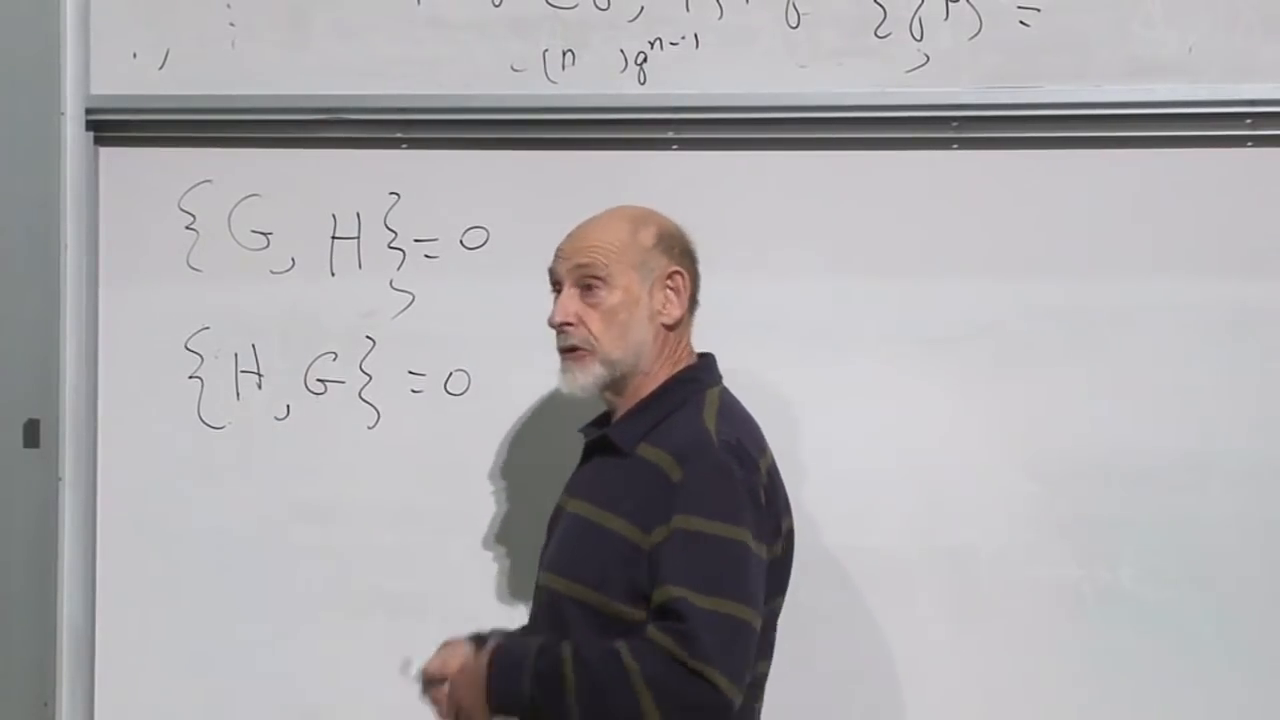
\includegraphics[width=0.82\textwidth]{lecture_08_figure_02.png}
  \caption{Три декартовы компоненты момента импульса и их компактная форма через векторное произведение.}
  \lectureframe{00:34:00}
\end{figure}

Вращение вокруг оси, заданной произвольным единичным вектором \(\boldsymbol n\), порождается
\begin{equation}
  L_{\boldsymbol n}=\boldsymbol n\cdot\boldsymbol L.
  \label{eq:l8-arbitrary-axis}
\end{equation}
Для изолированной вращательно-инвариантной системы сохраняются все три компоненты. Если симметрией остаются только вращения вокруг одной оси, то гарантированно сохраняется лишь компонента вдоль этой оси.

\section{Момент импульса порождает вращения}

Вместо того чтобы сразу решать задачу о вращательной динамике, исследуем, как \(L_z\) действует через скобку Пуассона. Используя
Eq.~\eqref{eq:l8-lz},
\begin{align}
  \{x,L_z\}
  &=\{x,xp_y-yp_x\}
   =-y\{x,p_x\}
   =-y,\\
  \{y,L_z\}
  &=\{y,xp_y-yp_x\}
   =x\{y,p_y\}
   =x,\\
  \{z,L_z\}&=0.
  \label{eq:l8-position-rotation-brackets}
\end{align}
Это в точности коэффициенты из
Eq.~\eqref{eq:l8-z-rotation}.

\begin{figure}[htbp]
  \centering
  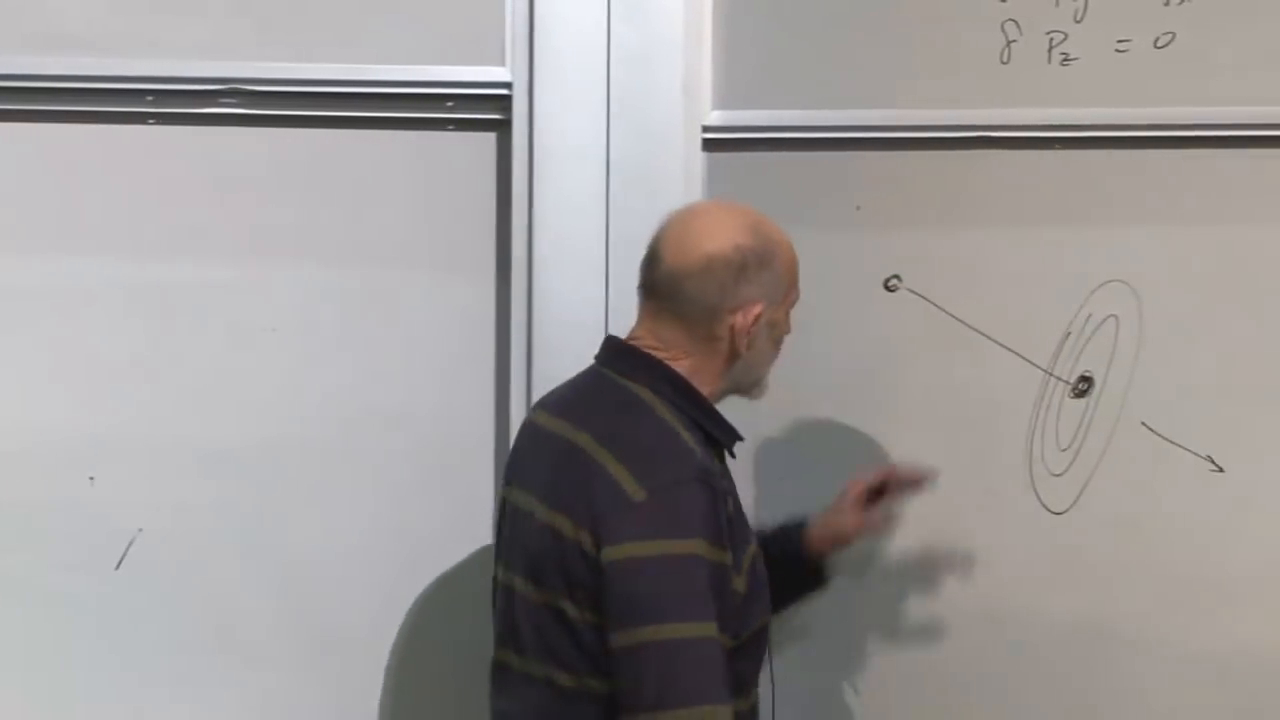
\includegraphics[width=0.82\textwidth]{lecture_08_figure_03.png}
  \caption{Скобки координат с \(L_z\): скобка воспроизводит бесконечно малый поворот \((x,y,z)\).}
  \lectureframe{00:38:41}
\end{figure}

Импульс тоже является вектором, и тот же расчёт даёт
\begin{equation}
  \begin{aligned}
    \{p_x,L_z\}&=-p_y,\\
    \{p_y,L_z\}&=p_x,\\
    \{p_z,L_z\}&=0.
  \end{aligned}
  \label{eq:l8-momentum-rotation-brackets}
\end{equation}

\begin{figure}[htbp]
  \centering
  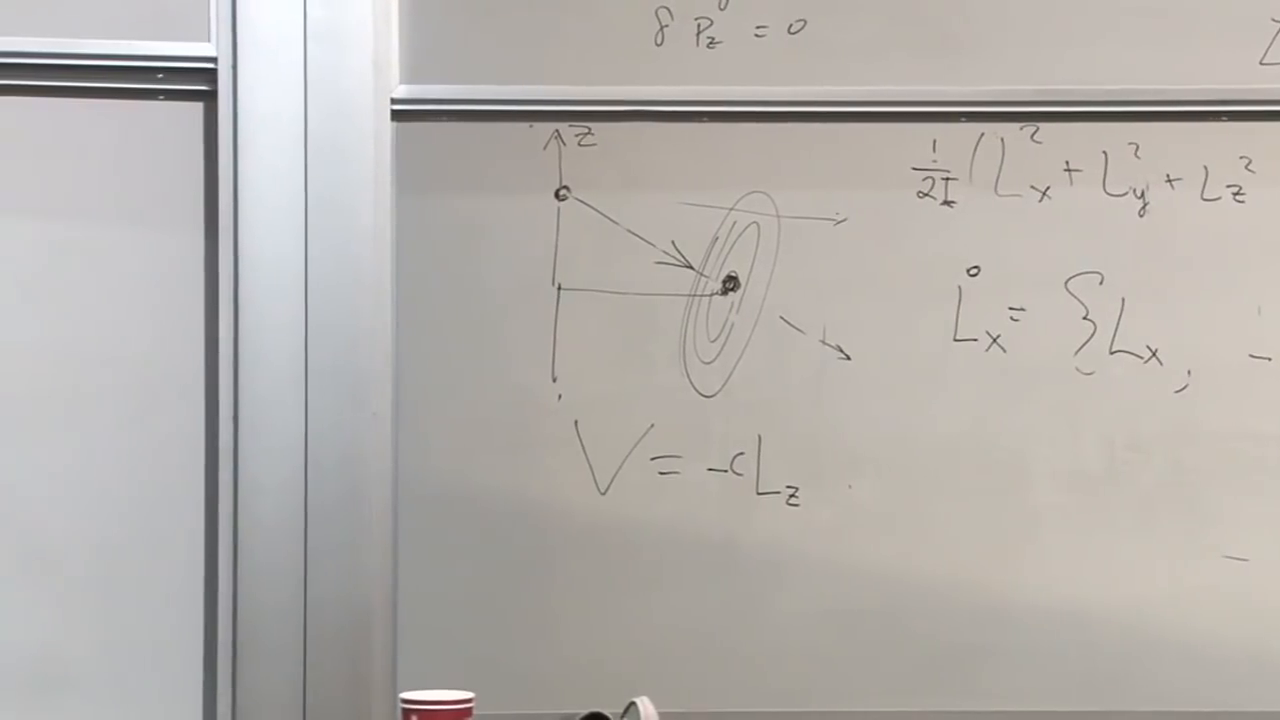
\includegraphics[width=0.82\textwidth]{lecture_08_figure_04.png}
  \caption{Положение и импульс преобразуются по одному и тому же векторному закону при вращении, порождаемом \(L_z\).}
  \lectureframe{00:42:08}
\end{figure}

Итак, общее утверждение гамильтоновой механики таково:
\begin{equation}
  \boxed{\delta_G A=\epsilon\{A,G\}.}
  \label{eq:l8-generator-rule}
\end{equation}
Каждая функция фазового пространства \(G\) задаёт такое бесконечно малое каноническое преобразование. Если \(G=L_z\), это вращение. Если \(G=H\), это малый шаг по времени.

\begin{classroomqa}
  \audiencequestion{В лекции иногда говорится о вращении системы и
  иногда — о вращении координат. Какое соглашение используется в уравнениях со скобками?
  \lecturetimestamp{00:28:22--00:29:35}}
  \lecturerresponse{Уравнение~\eqref{eq:l8-z-rotation} фиксирует соглашение:
  речь идёт об активном бесконечно малом повороте
  \((x,y)\mapsto(x-\epsilon y,y+\epsilon x)\). Пассивный поворот осей
  даёт противоположный знак. Как только соглашение зафиксировано, формулы со скобками становятся однозначными.}
\end{classroomqa}

\section{Импульс порождает трансляции}

Трансляция по одной координате имеет вид
\begin{equation}
  \delta q=\epsilon.
  \label{eq:l8-q-translation}
\end{equation}
Здесь \(F(q)=1\) в Eq.~\eqref{eq:l8-noether-variation}, поэтому соответствующая
сохраняющаяся величина — \(p\). Утверждение о генераторе предсказывает
\begin{equation}
  \{f(q),p\}=\frac{df}{dq}.
  \label{eq:l8-translation-derivative}
\end{equation}
В лекции это сначала доказывается для степеней методом индукции. База индукции —
\(\{q,p\}=1\). Предположим,
\begin{equation}
  \{q^{n-1},p\}=(n-1)q^{n-2}.
  \label{eq:l8-induction-hypothesis}
\end{equation}
Тогда правило произведения даёт
\begin{align}
  \{q^n,p\}
  &=\{q\,q^{n-1},p\}\\
  &=q\{q^{n-1},p\}+\{q,p\}q^{n-1}\\
  &=(n-1)q^{n-1}+q^{n-1}\\
  &=nq^{n-1}.
  \label{eq:l8-power-translation}
\end{align}
По линейности результат распространяется на многочлены и на сходящиеся представления степенными рядами.
Ещё прямее, определение скобки даёт
Eq.~\eqref{eq:l8-translation-derivative} для любой дифференцируемой \(f(q)\):
\begin{equation}
  \{f(q),p\}
  =
  \frac{\partial f}{\partial q}
  \frac{\partial p}{\partial p}
  =f'(q).
\end{equation}

\begin{figure}[htbp]
  \centering
  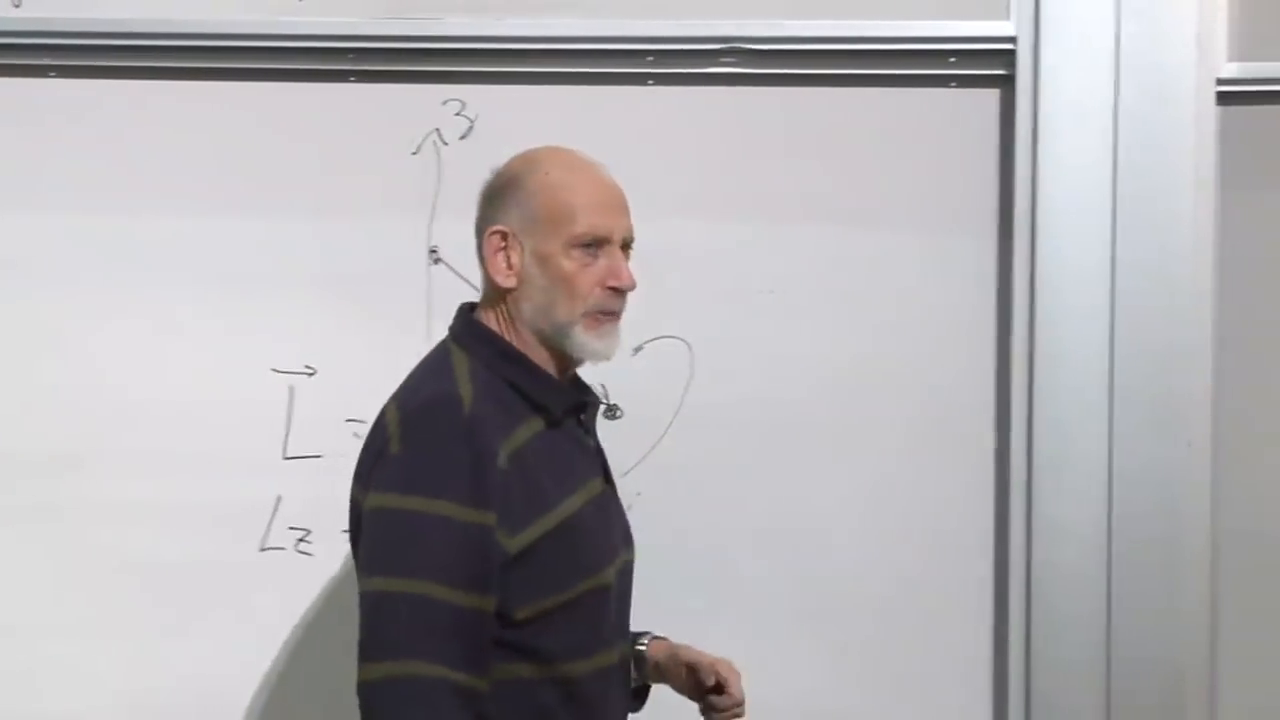
\includegraphics[width=0.82\textwidth]{lecture_08_figure_05.png}
  \caption{Результат для трансляции после индукционного доказательства:
  \(\{F(q),p\}=dF/dq\).}
  \lectureframe{00:53:18}
\end{figure}

Теперь мы увидели три варианта одной и той же идеи:
\begin{center}
  \begin{tabular}{@{}>{\raggedright\arraybackslash}p{0.37\textwidth}
                      >{\raggedright\arraybackslash}p{0.55\textwidth}@{}}
    \toprule
    Генератор и преобразование&Бесконечно малое действие\\
    \midrule
    \(H\), сдвиг по времени& \(\delta_tA=\epsilon\{A,H\}\)\\
    \(p_i\), пространственный сдвиг& \(\delta A=\epsilon\{A,p_i\}\)\\
    \(L_i\), вращение& \(\delta A=\epsilon\{A,L_i\}\)\\
    \bottomrule
  \end{tabular}
\end{center}
Сохраняющаяся величина, связанная с непрерывной симметрией, также является генератором этой симметрии.

\section{Одна скобка, два прочтения}

Пусть \(G(q,p)\) — предполагаемый генератор. Если он сохраняется и не имеет явной зависимости от времени, то
\begin{equation}
  \dot G=\{G,H\}=0.
  \label{eq:l8-g-conserved}
\end{equation}
По антисимметрии,
\begin{equation}
  \{H,G\}=0.
  \label{eq:l8-h-invariant}
\end{equation}
Эти уравнения математически эквивалентны, но их физический смысл различен:
\begin{itemize}
  \item \(\{G,H\}=0\) утверждает, что \(G\) не меняется при временной эволюции, порождённой \(H\).
  \item \(\{H,G\}=0\) утверждает, что \(H\) не меняется при преобразовании, порождённом \(G\).
\end{itemize}
Первое — закон сохранения; второе — симметрия гамильтониана. Связь Нётер здесь сжата до одного нуля.

\begin{figure}[htbp]
  \centering
  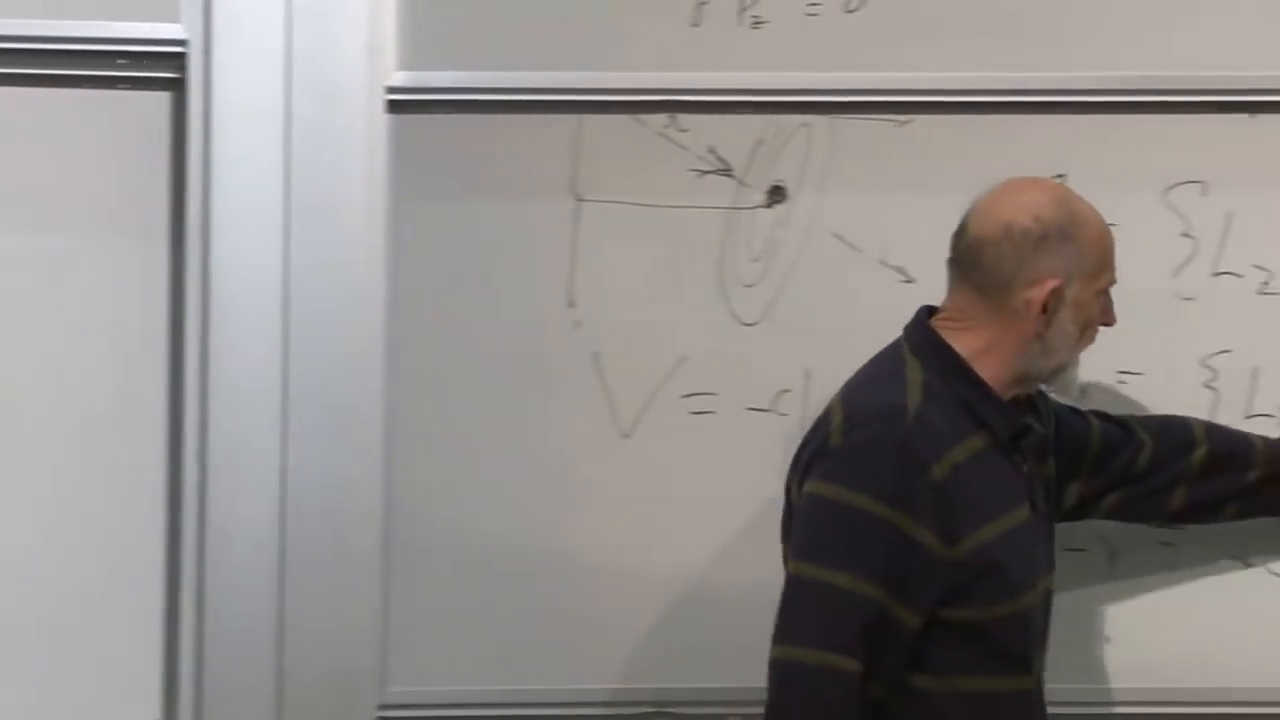
\includegraphics[width=0.82\textwidth]{lecture_08_figure_06.png}
  \caption{Два порядка одной и той же обращающейся в нуль скобки: сохранение \(G\) и инвариантность \(H\) относительно преобразования, порождённого \(G\).}
  \lectureframe{01:03:05}
\end{figure}

\begin{classroomqa}
  \audiencequestion{Если известна сохраняющаяся величина, всегда ли можно восстановить соответствующую симметрию? \lecturetimestamp{01:01:42--01:02:15}}
  \lecturerresponse{В рамках этой гамильтоновой постановки — да: возьмите скобку каждой переменной фазового пространства с \(G\). Совокупность соотношений \(\delta_GA=\epsilon\{A,G\}\) показывает, как преобразуются переменные. Например, скобки с \(L_z\) выявляют вращение, даже если такая интерпретация заранее не была известна. В более сложных постановках возможны глобальные и граничные тонкости, но здесь используется именно локальное инфинитезимальное утверждение.}
\end{classroomqa}

\begin{classroomqa}
  \audiencequestion{Говорят ли эти уравнения со скобками, какое физическое движение отвечает за закон сохранения?
  \lecturetimestamp{00:56:01--00:58:13}}
  \lecturerresponse{Нет. Они задают преобразование симметрии, а не фактическую траекторию. Сохранение \(L_z\) указывает на вращательную симметрию; оно не означает, что частица движется по окружности. Реальную временную эволюцию порождает \(H\). Скобка с другим генератором описывает другое направление преобразования в фазовом пространстве.}
\end{classroomqa}

\begin{classroomqa}
  \audiencequestion{Существует ли общее утверждение о преобразовании, которое не предполагает сохранения заранее? \lecturetimestamp{01:02:40--01:04:45}}
  \lecturerresponse{Да. Уравнение~\eqref{eq:l8-generator-rule} определяет инфинитезимальное преобразование для любой функции \(G\), независимо от того, сохраняется она или нет. Оно становится симметрией только тогда, когда гамильтониан инвариантен: \(\{H,G\}=0\). То же условие, прочитанное в обратном порядке, тогда утверждает, что \(G\) сохраняется.}
\end{classroomqa}

\section{Алгебра углового момента}

Следующее вычисление избавляет нас от необходимости протаскивать координаты частицы через каждую задачу о вращении. Начнём с
\[
  L_x=yp_z-zp_y,\qquad
  L_z=xp_y-yp_x.
\]
В \(\{L_x,L_z\}\) большинство перекрёстных членов обращается в нуль, потому что их индексы не образуют канонических пар. Оставшиеся свёртки дают
\begin{align}
  \{L_x,L_z\}
  &=\{yp_z-zp_y,xp_y-yp_x\}\\
  &=xp_z-zp_x\\
  &=-L_y.
  \label{eq:l8-lx-lz}
\end{align}
При обращении порядка минус исчезает. Циклическая перестановка координат даёт
\begin{equation}
  \boxed{\begin{aligned}
    \{L_x,L_y\}&=L_z,\\
    \{L_y,L_z\}&=L_x,\\
    \{L_z,L_x\}&=L_y.
  \end{aligned}}
  \label{eq:l8-angular-algebra}
\end{equation}
В индексной записи,
\begin{equation}
  \{L_i,L_j\}=\varepsilon_{ijk}L_k.
  \label{eq:l8-angular-algebra-index}
\end{equation}

\begin{figure}[htbp]
  \centering
  \includegraphics[width=0.82\textwidth]{lecture_08_figure_07.png}
  \caption{Циклическая алгебра скобок Пуассона трёх компонент углового момента.}
  \lectureframe{01:10:52}
\end{figure}

Этот результат можно было и предвидеть. Поскольку \(\boldsymbol L\) — вектор, скобка её \(x\)-компоненты с \(L_z\) должна давать инфинитезимальное изменение этой компоненты при вращении вокруг \(z\), а именно \(-L_y\). Явное вычисление подтверждает этот геометрический аргумент. Эти уравнения также являются классическими предшественниками квантовых коммутационных соотношений для углового момента.

\section{Быстрый гироскоп}

В качестве применения рассмотрим гироскоп: быстро вращающийся маховик, центр которого находится на фиксированном расстоянии \(R\) от точки опоры. Пусть \(\boldsymbol r\) направлен от опоры к центру колеса. Маховик вращается вокруг своей оси настолько быстро, что его основной угловой момент остаётся направленным вдоль этого направления. В приближении, используемом в лекции,
\begin{equation}
  \boldsymbol L=\ell\,\boldsymbol r,
  \qquad
  L_z=\ell z,
  \label{eq:l8-L-parallel-r}
\end{equation}
где \(\ell=L/R\) считается постоянной. Меньшими угловыми моментами, связанными с нутацией или движением оси, поначалу пренебрегают.

\begin{figure}[htbp]
  \centering
  \begin{tikzpicture}[scale=0.95,>=Latex]
    \coordinate (P) at (0,3.2);
    \coordinate (C) at (3.7,1.55);
    \draw[->] (0,-0.2) -- (0,4.35) node[above] {\(z\)};
    \fill (P) circle (1.7pt) node[left] {pivot};
    \draw[very thick,->] (P) -- (C)
      node[midway,above right] {\(\boldsymbol r\parallel\boldsymbol L\)};
    \fill (C) circle (1.7pt);
    \draw[dashed] (P) -- (0,1.55);
    \draw[dashed] (0,1.55) -- (C);
    \node[left] at (0,1.55) {\(z\)};
    \begin{scope}[shift={(C)},rotate=-24]
      \draw[very thick] (0,0) ellipse (0.65 and 1.35);
      \draw[thick] (0,0) ellipse (0.42 and 0.9);
    \end{scope}
    \draw[->,thick] (2.15,2.85)
      arc[start angle=140,end angle=35,radius=1.65];
  \end{tikzpicture}
  \caption{Приближение быстрого гироскопа. Расстояние от опоры до центра фиксировано, а доминирующий момент собственного вращения остаётся сонаправленным с осью и \(\boldsymbol r\).}
\end{figure}

\begin{figure}[htbp]
  \centering
  \includegraphics[width=0.82\textwidth]{lecture_08_figure_08.png}
  \caption{Эскиз маховика на доске вместе с \(H_{\rm rot}=L^2/(2I)\) и сокращением членов, доказывающим сохранение \(\boldsymbol L\) при отсутствии момента сил.}
  \lectureframe{01:18:54}
\end{figure}

\subsection{Без гравитации: почему каждая компонента остаётся постоянной}

Для упрощённого осесимметричного ротора
\begin{equation}
  H_{\mathrm{rot}}
  =\frac{1}{2I}
  \left(L_x^2+L_y^2+L_z^2\right)
  =\frac{L^2}{2I}.
  \label{eq:l8-rotational-hamiltonian}
\end{equation}
Коэффициент равен \(1/(2I)\), а не \(I/2\); на доске эта ошибка появляется и исправляется. Используя уравнение~\eqref{eq:l8-angular-algebra},
\begin{align}
  \dot L_x
  &=\{L_x,H_{\mathrm{rot}}\}\\
  &=\frac{1}{2I}\left(
    2L_y\{L_x,L_y\}
    +2L_z\{L_x,L_z\}
  \right)\\
  &=\frac{1}{I}\left(L_yL_z-L_zL_y\right)=0.
  \label{eq:l8-free-lx}
\end{align}
При циклической перестановке,
\begin{equation}
  \dot L_x=\dot L_y=\dot L_z=0.
  \label{eq:l8-free-angular-momentum}
\end{equation}
Скаляр \(L^2\) имеет нулевую скобку с каждой компонентой \(L_i\); на языке этой алгебры это элемент Казимира. Следовательно, гироскоп без момента сил сохраняет и модуль, и направление своего углового момента.

\begin{classroomqa}
  \audiencequestion{Является ли момент инерции здесь просто числом?
  \lecturetimestamp{01:14:23--01:15:05}}
  \lecturerresponse{Для этой редуцированной модели — да. Он кодирует распределение массы колеса относительно его оси вращения. Для общего твёрдого тела имеется тензор моментов инерции и вращательный гамильтониан \(\sum_i L_i^2/(2I_i)\) в главных осях. В лекции выбирается более простой быстрый симметричный ротор, потому что цель состоит в том, чтобы показать метод скобок Пуассона, а не развивать полную динамику твёрдого тела.}
\end{classroomqa}

\subsection{Гравитация и знак потенциала}

Выберем вертикальную координату \(z\) положительной вверх и поместим точку опоры в начало координат. Потенциальная энергия тяжести центра колеса равна
\begin{equation}
  V=Mgz.
  \label{eq:l8-mgz}
\end{equation}
Поскольку \(L_z=\ell z\),
\begin{equation}
  V=cL_z,
  \qquad
  c=\frac{Mg}{\ell}=\frac{MgR}{L}.
  \label{eq:l8-potential-lz}
\end{equation}
Здесь \(c>0\), если \(\boldsymbol L\) выбрано параллельным \(\boldsymbol r\). Если маховик вращается в противоположную сторону, знаковая связь между \(\boldsymbol L\) и \(\boldsymbol r\) меняется на противоположную, и то же происходит с соответствующей знаковой частотой прецессии.

\begin{figure}[htbp]
  \centering
  \includegraphics[width=0.82\textwidth]{lecture_08_figure_09.png}
  \caption{Геометрия при фиксированной длине, лежащая в основе \(\boldsymbol L=\ell\boldsymbol r\) и \(L_z=\ell z\).}
  \lectureframe{01:25:38}
\end{figure}

\begin{figure}[htbp]
  \centering
  \includegraphics[width=0.82\textwidth]{lecture_08_figure_10.png}
  \caption{На промежуточном этапе на доске записано \(V=-cL_z\). Позднее знак исправляется после того, как \(z\) фиксируется направленной вверх: при \(\boldsymbol L=\ell\boldsymbol r\) и \(\ell>0\) согласованный результат таков: \(V=+cL_z\).}
  \lectureframe{01:22:43}
\end{figure}

\begin{classroomqa}
  \audiencequestion{Почему высоту можно заменить компонентой углового момента? Наклонная линия — это ось или радиус-вектор?
  \lecturetimestamp{01:22:20--01:25:43}}
  \lecturerresponse{Наклонную линию лучше всего обозначить как \(\boldsymbol r\), вектор от закреплённой опоры к центру колеса. Реальная ось может лежать вдоль него, но соотношение, используемое в вычислении, — это приближение быстрого вращения \(\boldsymbol L=\ell\boldsymbol r\). Поэтому их \(z\)-компоненты пропорциональны. В живом обсуждении обозначения несколько раз меняются, прежде чем это различие окончательно фиксируется.}
\end{classroomqa}

\begin{classroomqa}
  \audiencequestion{Какие предположения делают \(\ell\) постоянной, и что перестаёт работать, если центр колеса может скользить радиально?
  \lecturetimestamp{01:25:43--01:26:38,\allowbreak\ 01:34:22--01:35:00}}
  \lecturerresponse{Предполагается, что доминирующий угловой момент собственного вращения намного больше углового момента, связанного с медленным движением, а расстояние от опоры до центра фиксировано. Тогда модуль собственного вращения мало меняется, и \(\boldsymbol L\) вращается вместе с \(\boldsymbol r\). Если бы центр мог скользить радиально, \(z\) уже не было бы пропорционально \(L_z\) с одним постоянным коэффициентом, так что редуцированный гамильтониан \(V=cL_z\) не описывал бы движение.}
\end{classroomqa}

\begin{classroomqa}
  \audiencequestion{Почему на доске сначала стоит минус, а позже плюс? Имеет ли направление вращения значение?
  \lecturetimestamp{01:27:13--01:28:15,\allowbreak\ 01:33:09--01:33:21}}
  \lecturerresponse{Начальный знак — это ошибка на доске по ходу лекции, смешанная с ещё не устоявшейся договорённостью о направлении оси. Как только \(z\) определяется направленной вверх, \(V=Mgz\) растёт с высотой. Если \(\boldsymbol L=\ell\boldsymbol r\) при \(\ell>0\), получаем \(V=+cL_z\). При обращении направления вращения меняются на противоположные знаковая пропорциональность и направление прецессии, но это не возвращает возможности произвольно выбирать знак.}
\end{classroomqa}

\subsection{Прецессия из трёх коротких уравнений}

Полный редуцированный гамильтониан имеет вид
\begin{equation}
  H=
  \frac{1}{2I}\left(L_x^2+L_y^2+L_z^2\right)+cL_z.
  \label{eq:l8-full-gyro-hamiltonian}
\end{equation}
Мы уже показали, что \(L^2\) имеет нулевую скобку с каждым \(L_i\). Вклад даёт только линейный член:
\begin{align}
  \dot L_z&=\{L_z,H\}=0,\\
  \dot L_x&=\{L_x,H\}=c\{L_x,L_z\}=-cL_y,\\
  \dot L_y&=\{L_y,H\}=c\{L_y,L_z\}=cL_x.
  \label{eq:l8-precession-equations}
\end{align}

\begin{figure}[htbp]
  \centering
  \includegraphics[width=0.82\textwidth]{lecture_08_figure_11.png}
  \caption{Итоговые уравнения для компонент: \(L_z\) постоянно, тогда как \(L_x\) и \(L_y\) переходят друг в друга при вращении.}
  \lectureframe{01:30:35}
\end{figure}

Вертикальная компонента и горизонтальный модуль постоянны:
\begin{equation}
  \frac{d}{dt}(L_x^2+L_y^2)
  =2L_x(-cL_y)+2L_y(cL_x)=0.
\end{equation}
Объединив горизонтальные компоненты,
\begin{equation}
  L_+=L_x+iL_y,
  \qquad
  \dot L_+=icL_+,
\end{equation}
поэтому
\begin{equation}
  L_+(t)=L_+(0)e^{ict}.
  \label{eq:l8-precession-solution}
\end{equation}
Следовательно, вектор углового момента прецессирует вокруг вертикальной оси с угловой скоростью \(|c|=MgR/L\). В этом идеализированном стационарном движении его наклон остаётся постоянным.

\begin{classroomqa}
  \audiencequestion{Был ли опущен член вращательной энергии, когда записывались уравнения прецессии?
  \lecturetimestamp{01:35:01--01:35:49}}
  \lecturerresponse{Нет. Он входит в полный гамильтониан, как в формуле~\eqref{eq:l8-full-gyro-hamiltonian}. Он просто даёт нулевой вклад в \(\dot L_i\), поскольку \(\{L_i,L^2\}=0\); это сокращение уже было доказано в расчёте без момента сил. Вопрос студента делает этот неявный шаг явным.}
\end{classroomqa}

\begin{classroomqa}
  \audiencequestion{Является ли равномерная прецессия равновесием? Что происходит после небольшого толчка? \lecturetimestamp{01:32:38--01:33:08}}
  \lecturerresponse{Её лучше называть установившимся или стационарным движением, а не статическим равновесием. Небольшой толчок, вообще говоря, добавляет нутацию, то есть колебание угла наклона. Для очень быстро вращающегося колеса это колебание мало, поэтому в сокращённом рассмотрении сохраняют только почти равномерную прецессию.}
\end{classroomqa}

\begin{classroomqa}
  \audiencequestion{Требует ли прецессия опоры или реальной оси?
  \lecturetimestamp{01:31:49--01:32:38,\allowbreak\ 01:33:49--01:35:00}}
  \lecturerresponse{В этой механической модели предполагается фиксированное расстояние от шарнира до центра, так что опору обеспечивает некоторая связь. Более глубокий алгебраический результат шире: всякий раз, когда гамильтониан содержит член, линейный по одной из компонент углового момента, та же алгебра скобок порождает прецессию. Микроскопический источник углового момента не обязан быть буквально колесом на оси.}
\end{classroomqa}

\begin{classroomqa}
  \audiencequestion{Это та же прецессия, что и у электронного или ядерного спина в магнитном поле, или у орбиты планеты?
  \lecturetimestamp{01:35:50--01:37:00}}
  \lecturerresponse{Магнитный момент, взаимодействующий с магнитным полем, имеет гамильтониан, линейный по компоненте спина, и потому подчиняется той же алгебре углового момента. Прецессия ядерного спина лежит в основе ядерного магнитного резонанса. Прецессия перигелия планетной орбиты — другое явление, которое лишь обозначается тем же словом \emph{прецессия}; это не тот же расчёт.}
\end{classroomqa}

\begin{classroomqa}
  \audiencequestion{Является ли гироскоп с боковым креплением по существу тем же самым объектом, что и волчок? \lecturetimestamp{01:37:02--01:37:23}}
  \lecturerresponse{Да. Различие в основном в геометрической терминологии: когда ось вращения выступает в сторону от опоры, обычно говорят о гироскопе; когда она почти вертикальна, говорят о волчке. Структура углового момента и момента сил одна и та же.}
\end{classroomqa}

\section{Что дал этот расчёт}

Углы Эйлера не вводились, и координаты каждой части колеса не отслеживались. Как только стало известно
\[
  \{L_i,L_j\}=\varepsilon_{ijk}L_k
\]
, уравнения для интересующих переменных следовали непосредственно.
В этом и состояла задуманная демонстрация силы метода. Осциллятор показал, что скобки Пуассона могут воспроизводить знакомую динамику. Угловой момент показал, что они способны на гораздо большее:
\begin{itemize}
  \item сохраняющаяся величина порождает соответствующую ей бесконечно малую симметрию;
  \item сохранение \(G\) и инвариантность \(H\) — два прочтения \(\{G,H\}=0\);
  \item алгебра наблюдаемых может замыкаться на себя, что позволяет решать динамику, не возвращаясь к микроскопическим координатам;
  \item гамильтониан, линейный по одной из компонент углового момента, порождает прецессию вокруг этой оси.
\end{itemize}
Лекция останавливается, не доходя до полных уравнений Эйлера для общего твёрдого тела. Её более узкий вывод уже завершён: правильно выбранные генераторы и их алгебра Пуассона с поразительной экономией выявляют и симметрию, и движение.
\chapter{Магнитные силы, векторные потенциалы и принцип действия}

\lectureoverview{Электростатические силы укладываются в привычную консервативную схему, но магнитные силы зависят от скорости. Чтобы включить их в лагранжеву механику, мы сначала развиваем необходимый векторный анализ, используем тот факт, что магнитное поле не имеет источников, чтобы ввести векторный потенциал, рассматриваем его калибровочную свободу, а затем строим магнитный член в действии.}

\section{Новый вид силы}

Предшествующее обсуждение момента импульса, гироскопов и скобок Пуассона свело воедино несколько тем. В частности, вращающееся заряженное тело в магнитном поле прецессирует почти так же, как гироскоп. Теперь мы переходим от этой аналогии к движению отдельной заряженной частицы.

Электростатические силы не требуют новой механики. Если \(U(\mathbf x)\) — потенциальная энергия, то
\begin{equation}
  \mathbf F=-\nabla U(\mathbf x),
\end{equation}
и обычный довод дает закон сохранения суммы кинетической и потенциальной энергий. Для частицы с зарядом \(e\) в электростатическом потенциале \(V(\mathbf x)\),
\begin{equation}
  U(\mathbf x)=eV(\mathbf x),
  \qquad
  \mathbf F_{\mathrm{el}}=-e\nabla V.
\end{equation}
Магнитные силы имеют другую форму. Они зависят от скорости частицы, поэтому их нельзя ввести просто добавлением еще одной обычной потенциальной энергии. Тем не менее они следуют из принципа действия и допускают как лагранжево, так и гамильтоново описание. Чтобы прийти к этому описанию, нужен короткий, но существенный экскурс в векторный анализ.

\section{Поля и локальные операции}

\subsection{Что фиксирует поле}

Поле сопоставляет физическую величину каждой точке пространства и, вообще говоря, каждому моменту времени. Температура и давление — скалярные поля. Скорость ветра — векторное поле. Электрическое и магнитное поля — векторные поля. В других теориях скалярные поля встречаются даже на микроскопических масштабах, тогда как гравитация описывается тензорным полем. В настоящем обсуждении мы опускаем всякую зависимость от времени и записываем поля как функции \(\mathbf x\).

Операциональный смысл поля состоит в локальности. Представьте, что некоторая область скрыта внутри мешка. Чтобы измерить электрическое поле в этой области, поместите туда малый пробный заряд и наблюдайте его ускорение. Сила определяется полем в той точке, где находится заряд, а не отдельным обращением к каждому далекому источнику. То же относится и к магнитному полю и движущемуся пробному заряду. Позднее векторный потенциал заставит нас уточнить эту простую картину, но начинать следует именно с нее.

\subsection{Оператор дифференцирования}

Производные превращают поля в другие поля. Мы объединяем три пространственные производные в
\begin{equation}
  \nabla
  =
  \left(
    \frac{\partial}{\partial x},
    \frac{\partial}{\partial y},
    \frac{\partial}{\partial z}
  \right).
\end{equation}
Символ читается как \emph{дель} или \emph{набла}. Его вид перевернутого треугольника легко запоминается, но его подлинное значение состоит в том, что формально он ведет себя как вектор, компонентами которого являются дифференциальные операторы.

Это обычное трехмерное физическое пространство, не фазовое пространство и не конфигурационное пространство многих частиц. Более того, \(\nabla\) — не векторное поле, которое может существовать само по себе. Оно должно действовать на что-то. Если \(T(\mathbf x)\) — скалярное поле температуры, то
\begin{equation}
  \nabla T
  =
  \left(
    \frac{\partial T}{\partial x},
    \frac{\partial T}{\partial y},
    \frac{\partial T}{\partial z}
  \right)
\end{equation}
есть его градиент, подлинное векторное поле.

\begin{figure}[htbp]
\centering
\includegraphics[width=0.82\textwidth]{lecture_09_figure_01.png}
\caption{На доске \(\nabla\) вводится как вектор операторов пространственных производных, после чего его начинают применять к скалярному полю \(T(\mathbf x)\).}
\lectureframe{00:11:30}
\end{figure}

Скаляр — это не просто величина, записанная одной компонентой. Это величина, значение которой не зависит от ориентации координатных осей. Стандартный пример — температура. Для данного векторного поля \(\mathbf E\) локальное выражение \(\mathbf E\cdot\mathbf E\) тоже является скаляром. Напротив, построение потенциала интегрированием поля — операция нелокальная; она использует значения вдоль пути.

\subsection{Дивергенция}

Для векторного поля \(\mathbf A=(A_x,A_y,A_z)\) скаляр
\begin{equation}
  \nabla\cdot\mathbf A
  =
  \frac{\partial A_x}{\partial x}
  +\frac{\partial A_y}{\partial y}
  +\frac{\partial A_z}{\partial z}
\end{equation}
является его дивергенцией. Говоря на языке гидродинамики, положительная дивергенция измеряет локальную тенденцию течь наружу, тогда как отрицательная измеряет тенденцию сходиться внутрь. Источник жидкости создает положительную дивергенцию; сток создает отрицательную. Эта картина качественна, но она сделает наглядным отсутствие источников у магнитного поля.

\section{Векторные произведения, символы эпсилон и ротор}

\subsection{Векторное произведение в компонентах}

Для двух векторов \(\mathbf V\) и \(\mathbf A\) одна из компонент векторного произведения имеет вид
\begin{equation}
  (\mathbf V\times\mathbf A)_x
  =
  V_yA_z-V_zA_y.
\end{equation}
Остальные две получаются циклической заменой \(x\to y\to z\to x\). Полезно заменить \(x,y,z\) индексами \(1,2,3\). Символ Кронекера равен
\begin{equation}
  \delta_{ij}
  =
  \begin{cases}
    1,&i=j,\\
    0,&i\ne j,
  \end{cases}
\end{equation}
а символ Леви--Чивиты определяется как
\begin{equation}
  \epsilon_{123}=\epsilon_{231}=\epsilon_{312}=1,
  \qquad
  \epsilon_{132}=\epsilon_{321}=\epsilon_{213}=-1,
\end{equation}
причем \(\epsilon_{ijk}=0\), если совпадают любые два индекса. Циклический обход по циферблату с тремя делениями дает знаки плюс; обход в обратном направлении дает знаки минус. Перестановка любой пары индексов меняет знак, так что \(\epsilon_{ijk}\) полностью антисимметричен.

Мы также используем соглашение о суммировании: индекс, повторяющийся в одном члене, суммируется от \(1\) до \(3\). Тогда три уравнения для векторного произведения принимают вид
\begin{equation}
  (\mathbf V\times\mathbf A)_i
  =
  \epsilon_{ijk}V_jA_k.
\end{equation}
Например, при \(i=1\) остаются только \((j,k)=(2,3)\) и \((3,2)\):
\begin{equation}
  (\mathbf V\times\mathbf A)_1
  =
  \epsilon_{123}V_2A_3
  +\epsilon_{132}V_3A_2
  =
  V_2A_3-V_3A_2.
\end{equation}
Следовательно, компактная запись в точности содержит привычное покомпонентное правило.

\subsection{Вектор под видом антисимметричной матрицы}

Существует и второе представление:
\begin{equation}
  V_iA_j-V_jA_i
  =
  \epsilon_{ijk}(\mathbf V\times\mathbf A)_k.
\end{equation}
Левая часть имеет два индекса и антисимметрична при \(i\leftrightarrow j\). В виде матрицы она имеет вид
\begin{equation}
  M_{ij}
  =
  \begin{pmatrix}
    0&M_{12}&M_{13}\\
    -M_{12}&0&M_{23}\\
    -M_{13}&-M_{23}&0
  \end{pmatrix}.
\end{equation}
Диагональные элементы равны нулю, а нижний треугольник определяется верхним. Поэтому имеется три независимые компоненты.

\begin{figure}[htbp]
\centering
\includegraphics[width=0.82\textwidth]{lecture_09_figure_02.png}
\caption{Одна компонента векторного произведения и схематический антисимметричный массив \(3\times3\), используемый для подсчета его независимых компонент. Пометки в клетках служат мнемоникой, а не дополнительными символами.}
\lectureframe{00:34:20}
\end{figure}

\begin{classroomqa}
\audiencequestion{Имеет ли векторное произведение, или отождествление с другим вектором, смысл вне трех измерений?}
\lecturerresponse{Антисимметричный объект с двумя индексами имеет смысл при любом числе измерений, но его отождествление с вектором является особенностью трех измерений. Вектор в трех измерениях имеет три компоненты, и антисимметричная матрица \(3\times3\) имеет три независимые компоненты. В четырех измерениях соответствующие числа равны 4 и 6, поскольку \(4(4-1)/2=6\). Антисимметричный объект по-прежнему существует и естественным образом рассматривается как 2-форма, но он не является еще одним четырехвектором.}
\end{classroomqa}

\subsection{Ротор}

Замена \(\mathbf V\) на \(\nabla\) определяет ротор:
\begin{equation}
  (\nabla\times\mathbf A)_i
  =
  \epsilon_{ijk}\frac{\partial A_k}{\partial x_j}.
\end{equation}
В обычных компонентах,
\begin{align}
  (\nabla\times\mathbf A)_x
  &=
  \frac{\partial A_z}{\partial y}
  -\frac{\partial A_y}{\partial z},\\
  (\nabla\times\mathbf A)_y
  &=
  \frac{\partial A_x}{\partial z}
  -\frac{\partial A_z}{\partial x},\\
  (\nabla\times\mathbf A)_z
  &=
  \frac{\partial A_y}{\partial x}
  -\frac{\partial A_x}{\partial y}.
\end{align}
Тогда как дивергенция измеряет локальное растекание, ротор измеряет локальную циркуляцию. У жидкости, вращающейся вокруг оси, ротор вдоль этой оси отличен от нуля. Эта картина особенно наглядна для полей скорости, хотя определение применимо к любому векторному полю.

\section{Два структурных тождества}

Почти вся математическая работа сводится к двум фактам:
\begin{equation}
  \nabla\cdot(\nabla\times\mathbf A)=0,
  \qquad
  \nabla\times(\nabla s)=0.
\end{equation}
Первое следует из того, что вторые производные симметричны, тогда как \(\epsilon_{ijk}\) антисимметричен:
\begin{equation}
  \nabla\cdot(\nabla\times\mathbf A)
  =
  \epsilon_{ijk}\partial_i\partial_j A_k
  =0.
\end{equation}
Второе следует из равенства смешанных частных производных:
\begin{equation}
  \bigl[\nabla\times(\nabla s)\bigr]_i
  =
  \epsilon_{ijk}\partial_j\partial_k s
  =0.
\end{equation}

\begin{figure}[htbp]
\centering
\includegraphics[width=0.80\textwidth]{lecture_09_figure_03.png}
\caption{Первое тождество на доске: дивергенция любого ротора равна нулю.}
\lectureframe{00:38:26}
\end{figure}

Это легкие направления, подходящие для обещанного на лекции домашнего задания или внезапной контрольной. Обратные утверждения требуют большей аккуратности. Локально или, глобально, на подходящей односвязной или стягиваемой области,
\begin{align}
  \nabla\cdot\mathbf F=0
  &\quad\Longrightarrow\quad
  \mathbf F=\nabla\times\mathbf A,\\
  \nabla\times\mathbf F=0
  &\quad\Longrightarrow\quad
  \mathbf F=\nabla s.
\end{align}
Без оговорки об области дыры и другие глобальные топологические особенности могут препятствовать этим выводам. В лекции используется локальная форма, и именно она нужна ниже.

\section{Почему магнитное поле является ротором}

\subsection{Отсутствие наблюдаемых магнитных источников}

Магнитное поле \(\mathbf B\) определяется операционально через его действие на заряженные частицы и токи. В обычном электромагнетизме без магнитных монополей,
\begin{equation}
  \nabla\cdot\mathbf B=0.
\end{equation}
Это отличается от электрического поля, дивергенция которого пропорциональна плотности электрического заряда. Электрические заряды являются источниками и стоками электрического потока. Никакого изолированного источника или стока магнитного потока не наблюдалось.

Магнитные монополи изменили бы это уравнение. Теории единого поля нередко дают теоретические основания ожидать существования таких объектов, но, если они существуют, их масса может быть слишком велика, чтобы их можно было породить в доступных экспериментах. Поэтому в настоящей теории плотность магнитного заряда принимается равной нулю.

\begin{classroomqa}
\audiencequestion{Что такое магнитный монополь? У обычных магнитов уже есть северный и южный полюса.}
\lecturerresponse{Изолированный монополь был бы подлинным источником или стоком магнитного поля, аналогично электрическому заряду. Обычный стержневой магнит устроен иначе. Линии поля, выходящие вблизи его северного полюса, изгибаются в пространстве и возвращаются через южный полюс, продолжаясь внутри материала магнита. То, что снаружи выглядит как источник и сток, на самом деле соединено, как жидкость, текущая по скрытой трубе. Никакого суммарного рождения или уничтожения магнитного потока нет.}
\end{classroomqa}

\begin{figure}[htbp]
\centering
\includegraphics[width=0.76\textwidth]{lecture_09_figure_04.png}
\caption{На доске противопоставлены кажущиеся северный и южный источники, при этом их силовые линии соединены через магнит, что подчеркивает: магнитный поток там не начинается и не заканчивается.}
\lectureframe{00:44:56}
\end{figure}

Поскольку \(\mathbf B\) бездивергентно, обратная теорема позволяет записать, по крайней мере локально,
\begin{equation}
  \boxed{\mathbf B=\nabla\times\mathbf A}.
\end{equation}
Поле \(\mathbf A\) — это векторный потенциал. Поначалу это может выглядеть как ненужное переописание измеримого поля \(\mathbf B\). Его назначение станет ясным лишь тогда, когда мы построим действие.

\subsection{Векторный потенциал не единственен}

Если \(\mathbf A\) — один из векторных потенциалов, то
\begin{equation}
  \mathbf A'=\mathbf A+\nabla s
\end{equation}
— тоже векторный потенциал, поскольку
\begin{equation}
  \nabla\times\mathbf A'
  =
  \nabla\times\mathbf A+\nabla\times(\nabla s)
  =
  \mathbf B.
\end{equation}
Такая замена называется \emph{калибровочным преобразованием}. Магнитное поле калибровочно-инвариантно.

\begin{figure}[htbp]
\centering
\includegraphics[width=0.80\textwidth]{lecture_09_figure_05.png}
\caption{На доске рядом записаны определяющее соотношение \(\mathbf B=\nabla\times\mathbf A\) и калибровочный сдвиг \(\mathbf A'=\mathbf A+\nabla s\).}
\lectureframe{01:03:01}
\end{figure}

Его произносят \emph{gauge}, а не \emph{gouache} и не \emph{gouge}--различие, на котором в лекции с притворной строгостью настаивают. Само слово историческое. Оно возникло в ранней попытке связать эту свободу со сравнением эталонов длины в разных местах; исходная интерпретация не сохранилась, а название осталось.

\begin{classroomqa}
\audiencequestion{В этом обсуждении калибровочное преобразование означает именно \(\mathbf A\mapsto\mathbf A+\nabla s\)?}
\lecturerresponse{Да. Именно это и есть полное электромагнитное преобразование, используемое здесь. Калибровочные преобразования в теории Янга--Миллса и других теориях поля обобщают ту же идею, но в электромагнетизме требуется только добавление градиента скалярной функции.}
\end{classroomqa}

Неединственность также проясняет, что именно непосредственно измеримо. Заряженная частица в малой области реагирует на локальное \(\mathbf B\), и все векторные потенциалы, связанные калибровочным преобразованием, предсказывают там одну и ту же силу. Не существует локального эксперимента такого классического типа, который приписывал бы \(\mathbf A\) единственное значение.

\begin{classroomqa}
\audiencequestion{Является ли добавление градиента полным описанием этой неединственности?}
\lecturerresponse{Локально, в односвязной области, да. Если \(\nabla\times\mathbf A'=\nabla\times\mathbf A\), то \(\nabla\times(\mathbf A'-\mathbf A)=0\), так что разность является градиентом. Глобально многосвязная область может вносить дополнительные тонкости. Добавление постоянного вектора уже включено в это описание, поскольку постоянный вектор является градиентом линейной скалярной функции. Добавление константы к самой \(s\) ничего не меняет, потому что её градиент исчезает.}
\end{classroomqa}

\begin{classroomqa}
\audiencequestion{Если у калибровочной свободы есть лежащая в основе физическая причина, то в чём она состоит?}
\lecturerresponse{Лекция откладывает эту более глубокую интерпретацию. Полезный первый шаг — работать с этой свободой и увидеть, как она входит в действие. Когда формализм станет привычным, будет легче распознать, почему калибровочные описания незаменимы.}
\end{classroomqa}

\section{Одно магнитное поле, много потенциалов}

Рассмотрим простейший возможный пример,
\begin{equation}
  \mathbf B=b\,\hat{\mathbf z},
  \qquad
  B_x=B_y=0,
  \qquad
  B_z=b,
\end{equation}
где \(b\) — константа. Один из векторных потенциалов имеет вид
\begin{equation}
  \mathbf A^{(1)}=(0,bx,0).
\end{equation}
В самом деле,
\begin{equation}
  (\nabla\times\mathbf A^{(1)})_z
  =
  \frac{\partial A_y^{(1)}}{\partial x}
  -\frac{\partial A_x^{(1)}}{\partial y}
  =b,
\end{equation}
а остальные компоненты ротора равны нулю.

Этот выбор, по-видимому, выделяет направление \(y\), хотя физическое поле обладает вращательной симметрией в плоскости \(x\)-\(y\). Второй выбор делает произвольность явной:
\begin{equation}
  \mathbf A^{(2)}=(-by,0,0).
\end{equation}
Он даёт
\begin{equation}
  (\nabla\times\mathbf A^{(2)})_z
  =
  0-\frac{\partial(-by)}{\partial y}
  =b.
\end{equation}
Два потенциала отличаются на
\begin{equation}
  \mathbf A^{(2)}-\mathbf A^{(1)}
  =
  (-by,-bx,0)
  =
  \nabla(-bxy).
\end{equation}
Следовательно, они калибровочно эквивалентны. Вращательно-симметричный выбор,
\begin{equation}
  \mathbf A^{(\mathrm{sym})}
  =
  \frac12\,\mathbf B\times\mathbf r
  =
  \left(-\frac{by}{2},\frac{bx}{2},0\right),
\end{equation}
— ещё один представитель того же семейства.

\begin{figure}[htbp]
\centering
\includegraphics[width=0.80\textwidth]{lecture_09_figure_06.png}
\caption{На двух фрагментах доски записаны варианты \(A_y=bx\) и \(A_x=-by\), оба дающие одно и то же однородное поле \(B_z=b\).}
\lectureframe{01:07:20}
\end{figure}

\begin{classroomqa}
\audiencequestion{Является ли это той же неоднозначностью, что и при различной расстановке катушек с током для создания поля?}
\lecturerresponse{Нет. Разные распределения тока — это разные физические источники, и они могут создавать в других местах разные поля, даже если в одной области совпадают. Калибровочная свобода остаётся и после того, как магнитное поле задано всюду: одно и то же физическое \(\mathbf B\) всё ещё имеет много векторных потенциалов.}
\end{classroomqa}

\begin{classroomqa}
\audiencequestion{Можно ли представлять добавление градиента как растяжение или сжатие без добавления закрутки?}
\lecturerresponse{Это полезная геометрическая интуиция. Ротор выявляет локальную закручивающую часть, а чистый градиент имеет нулевой ротор. Это утверждение в точности выражается равенством \(\nabla\times\nabla s=0\).}
\end{classroomqa}

\begin{classroomqa}
\audiencequestion{Существует ли фиксированное соотношение между направлением \(\mathbf A\) и направлением \(\mathbf B\)?}
\lecturerresponse{Никакого калибровочно-независимого соотношения не существует. В приведённых выше примерах просто так получилось, что \(A_z=0\), но к \(A_z\) можно было бы прибавить константу, не изменив ни одной производной. Тогда \(\mathbf A\) уже не был бы перпендикулярен \(\mathbf B\). В этом классическом обсуждении инвариантное физическое содержание имеет только ротор.}
\end{classroomqa}

В электростатике есть более слабый аналог. Поскольку \(\mathbf E=-\nabla V\), замена \(V\) на \(V+C\) не изменяет \(\mathbf E\). Термин \emph{векторный потенциал} был выбран отчасти по аналогии с этой свободой в обычном скалярном потенциале: потенциал можно изменить так, что физическое поле останется тем же.

\section{Сила Лоренца}

Теперь мы можем сформулировать закон силы, который должен воспроизвести принцип действия. В используемых здесь соглашениях
\begin{equation}
  \boxed{
  \mathbf F
  =
  e\left(
    \mathbf E+\frac{\mathbf v}{c}\times\mathbf B
  \right)
  =
  -e\nabla V+\frac{e}{c}\mathbf v\times\mathbf B
  }.
\end{equation}
Символ \(e\) — это электрический заряд частицы, \(\mathbf v=\dot{\mathbf x}\) — её скорость, а \(V\) — скалярный потенциал. Эта запись не должна побуждать нас спутать \(V\) с \(\mathbf v\). В системе SI \(V\) измеряется в вольтах, а \(e\) — в кулонах; показанный множитель \(1/c\) относится к соглашению о единицах, используемому в лекции. Существенный структурный момент не зависит от выбора единиц.

\begin{figure}[htbp]
\centering
\includegraphics[width=0.82\textwidth]{lecture_09_figure_07.png}
\caption{Электрический и магнитный члены силы Лоренца показаны вместе. Магнитный вклад пропорционален \(\mathbf v\times\mathbf B\).}
\lectureframe{00:58:54}
\end{figure}

Электрический член консервативен и уже знаком. Магнитный член здесь новый. Он обращается в нуль для покоящейся частицы и перпендикулярен и \(\mathbf v\), и \(\mathbf B\). Следовательно,
\begin{equation}
  \mathbf v\cdot\mathbf F_{\mathrm{mag}}
  =
  \frac{e}{c}\mathbf v\cdot(\mathbf v\times\mathbf B)
  =0.
\end{equation}
Статическое магнитное поле искривляет траекторию, но не совершает над частицей работы. Это не похоже на вязкое сопротивление, которое направлено противоположно скорости и отнимает кинетическую энергию.

Множитель \(v/c\) также показывает, почему при сопоставимых масштабах полей в этих соглашениях магнитные эффекты для медленно движущихся частиц часто меньше электрических. Электроны достаточно легки, чтобы достигать больших скоростей, поэтому магнитное отклонение по-прежнему легко наблюдать.

Исторически силы, действующие на проводники с током, были известны раньше, чем была выделена сила, действующая на отдельный заряд. Лоренц понял, что силу, действующую на проводник, можно объяснить, приписав скоростезависимый член каждому движущемуся заряду. Полное выражение, включающее электрическую и магнитную части, теперь называется законом силы Лоренца, хотя в нынешнем обсуждении новым является именно магнитный член.

\begin{classroomqa}
\audiencequestion{Есть ли у всего выражения отдельное обозначение, или силой Лоренца называется только магнитная часть?}
\lecturerresponse{Всё выражение — это просто сила \(\mathbf F=m\mathbf a\), и обычно именно его называют силой Лоренца. Магнитный член — часть, исторически наиболее непосредственно связанная с Лоренцем. Электрические и магнитные поля глубоко связаны относительностью, но это объединение не нужно для данной механической задачи.}
\end{classroomqa}

\subsection{Аналогия с силой Кориолиса}

Мы уже встречали векторное произведение скорости с фиксированным вектором. В системе отсчёта, вращающейся с угловой скоростью \(\boldsymbol\omega\), силу Кориолиса можно записать в виде
\begin{equation}
  \mathbf F_{\mathrm{Cor}}
  =
  2m\,\mathbf v\times\boldsymbol\omega.
\end{equation}
Она имеет ту же алгебраическую форму, что и магнитная сила:
\begin{equation}
  2m\boldsymbol\omega
  \quad\longleftrightarrow\quad
  \frac{e}{c}\mathbf B.
\end{equation}
Поэтому однородное магнитное поле, перпендикулярное плоскости, искривляет траектории заряженных частиц почти так же, как вращающаяся система отсчёта отклоняет движущиеся тела.

\begin{figure}[htbp]
\centering
\includegraphics[width=0.82\textwidth]{lecture_09_figure_08.png}
\caption{Слева остаётся сила Лоренца, а на доске добавляется соответствующая форма Кориолиса \(2m\,\mathbf v\times\boldsymbol\omega\).}
\lectureframe{01:02:08}
\end{figure}

\begin{classroomqa}
\audiencequestion{Силу Кориолиса называют фиктивной. Не является ли она менее реальной, чем магнитная сила, потому что зависит от скорости?}
\lecturerresponse{Зависимость от скорости здесь несущественна. Человек на вращающейся платформе может удерживать движущийся предмет и ощущать силу Кориолиса. Ее называют фиктивной, потому что в инерциальной системе отсчета она исчезает, тогда как вращающаяся система отсчета определяется именно наличием таких инерциальных членов. Слово \emph{реальная} часто менее полезно, чем указание, какая система отсчета и какое уравнение используются.}
\end{classroomqa}

Эту аналогию можно развить в небольшой мысленный эксперимент. На вращающейся платформе подходящее электростатическое поле может компенсировать центробежный член для выбранной частицы, тогда как подходящее однородное магнитное поле может компенсировать член Кориолиса. Такая компенсация работает только для выбранного отношения заряда к массе: электрические и магнитные силы масштабируются с \(e\), тогда как инерциальные силы масштабируются с \(m\). Конфигурация поля, настроенная на электроны, не компенсировала бы те же члены для частиц с другим \(e/m\).

\section{Построение действия для заряженной частицы}

\subsection{Стационарность действия при фиксированных концах}

Теперь мы задаем центральный вопрос: можно ли вывести силу Лоренца из принципа действия? Ответ положителен, но векторный потенциал незаменим. Лагранжиан, локально построенный только из частицы и \(\mathbf B\), не дает требуемой магнитной силы. Вместо того чтобы доказывать это отрицательное утверждение, мы сразу построим действие, которое работает.

Для траектории \(\mathbf x(t)\) запишем
\begin{equation}
  S[\mathbf x]
  =
  \int_{t_i}^{t_f}L(\mathbf x,\dot{\mathbf x},t)\,dt.
\end{equation}
В лекции для действия и векторного потенциала используется одна и та же рукописная буква, но мы будем обозначать действие через \(S\), а векторный потенциал через \(\mathbf A\). Физическая траектория делает \(S\) стационарным относительно вариаций, удерживающих оба конца фиксированными. Традиционное выражение \emph{наименьшее действие} удобно, хотя термин «стационарное действие» точнее, поскольку экстремум не обязан быть минимумом.

Фиксированность концов существенна. Можно представить, что концы пути прибиты к доске, а внутренняя часть слегка деформируется. Это траектория в обычной механике, а не объект теории струн; образ струны служит лишь способом наглядно представить вариацию.

\subsection{Что может входить в лагранжиан?}

При отсутствии всех полей лагранжиан равен кинетической энергии,
\begin{equation}
  L_0=\frac{m}{2}\dot{\mathbf x}^{\,2}.
\end{equation}
Электростатический член тоже стандартен:
\begin{equation}
  L_{\mathrm{el}}=-eV(\mathbf x).
\end{equation}
Магнитный член должен удовлетворять нескольким условиям:
\begin{enumerate}
  \item быть пропорциональным заряду \(e\);
  \item содержать множитель \(1/c\) в единицах, используемых в лекции;
  \item содержать скорость;
  \item быть скаляром относительно вращений.
\end{enumerate}

Соблазнительный пробный член \(\mathbf B\cdot\dot{\mathbf x}\) является скаляром и содержит скорость, но приводит к неверному уравнению движения. Правильный член использует векторный потенциал:
\begin{equation}
  L_{\mathrm{mag}}
  =
  \frac{e}{c}\mathbf A(\mathbf x)\cdot\dot{\mathbf x}
  =
  \frac{e}{c}A_i(\mathbf x)\dot x_i.
\end{equation}
Таким образом, полный не зависящий от времени электромагнитный лагранжиан имеет вид
\begin{equation}
  \boxed{
  L
  =
  \frac{m}{2}\dot{\mathbf x}^{\,2}
  +\frac{e}{c}\mathbf A(\mathbf x)\cdot\dot{\mathbf x}
  -eV(\mathbf x)
  }.
\end{equation}
В лекции 10 будут применены уравнения Эйлера--Лагранжа и явно показано, что это выражение дает силу Лоренца.

\begin{figure}[htbp]
\centering
\includegraphics[width=0.82\textwidth]{lecture_09_figure_09.png}
\caption{Завершенное построение действия на доске: свободный кинетический член плюс \((e/c)A_i\dot x_i\).}
\lectureframe{01:26:36}
\end{figure}

\section{Калибровочные преобразования меняют только конечные точки}

Магнитный вклад в действие равен
\begin{equation}
  S_{\mathrm{mag}}
  =
  \frac{e}{c}
  \int_{t_i}^{t_f}A_i(\mathbf x)\dot x_i\,dt.
\end{equation}
Поскольку \(\dot x_i\,dt=dx_i\), это криволинейный интеграл вдоль пути частицы \(\gamma\):
\begin{equation}
  S_{\mathrm{mag}}
  =
  \frac{e}{c}\int_\gamma A_i\,dx_i
  =
  \frac{e}{c}\int_\gamma\mathbf A\cdot d\mathbf x.
\end{equation}
Разбейте путь на короткие отрезки, возьмите компоненту \(\mathbf A\) вдоль каждого отрезка, умножьте на длину отрезка и сложите. Таков геометрический смысл этого интеграла.

Теперь выполним калибровочное преобразование
\begin{equation}
  A_i\longmapsto A_i+\partial_i s.
\end{equation}
Действие изменяется на
\begin{align}
  \Delta S
  &=
  \frac{e}{c}\int_\gamma \partial_i s\,dx_i\\
  &=
  \frac{e}{c}\int_\gamma ds\\
  &=
  \frac{e}{c}
  \left[
    s(\mathbf x_f)-s(\mathbf x_i)
  \right].
\end{align}
Каждый бесконечно малый отрезок дает значение \(s\) на одном конце минус его значение на другом. При суммировании все внутренние вклады телескопически сокращаются, и остаются только две конечные точки.

\begin{figure}[htbp]
\centering
\includegraphics[width=0.82\textwidth]{lecture_09_figure_10.png}
\caption{Криволинейный интеграл, его разбиение на малые участки пути и результат на концах \(s(\mathbf x_f)-s(\mathbf x_i)\).}
\lectureframe{01:32:31}
\end{figure}

\begin{classroomqa}
\audiencequestion{Если действие меняется при калибровочном преобразовании, почему траектория не меняется?}
\lecturerresponse{Принцип действия сравнивает пути при фиксированных начальной и конечной точках. Добавляемая величина зависит только от этих концов, поэтому для любого пути в данном сравнении она имеет одно и то же значение. Ее вариация равна нулю. Численное значение действия не является строго инвариантным, но уравнения Эйлера--Лагранжа и физическая траектория калибровочно инвариантны.}
\end{classroomqa}

Это различие — главный концептуальный результат лекции:
\begin{equation}
  \begin{aligned}
    S&\ \hbox{may shift by an endpoint term},\\
    \delta S&\ \hbox{and the equations of motion do not}.
  \end{aligned}
\end{equation}
Следовательно, калибровочная свобода совместима с принципом действия. Векторный потенциал может входить в лагранжиан, хотя магнитное поле не выделяет единственного \(\mathbf A\).

\section{Как продолжается рассуждение}

В этой лекции собраны необходимые средства и само действие, но она намеренно останавливается до варьирования этого действия. Следующие шаги теперь определены:
\begin{enumerate}
  \item применить уравнения Эйлера--Лагранжа и получить
  \(\mathbf F_{\mathrm{mag}}=(e/c)\mathbf v\times\mathbf B\);
  \item вычислить канонический импульс, который будет отличаться от \(m\mathbf v\);
  \item построить гамильтониан;
  \item выявить законы сохранения;
  \item решить задачу о движении заряженной частицы в однородном магнитном поле.
\end{enumerate}

Путь к этим результатам объясняет, зачем был введен векторный потенциал. Магнитное поле — это локально измеримый ротор, но векторный потенциал — объект, который естественным образом сопрягается с траекторией частицы. Калибровочные преобразования изменяют это сопряжение только на фиксированных концах, оставляя механику неизменной.

\chapter{Калибровочная инвариантность и движение заряженной частицы}

\lectureoverview{Магнитное поле имеет нулевую дивергенцию, поэтому его можно представить с помощью векторного потенциала. Это представление не единственно, однако именно оно позволяет включить магнитные силы в принцип действия. Мы выводим силу Лоренца, различаем канонический и механический импульсы, строим гамильтониан и используем две разные калибровки, чтобы решить задачу о движении в однородном магнитном поле. Лекция завершается рассмотрением того, как эта механика частицы вписывается в более широкий круг вопросов теории Максвелла, магнитных монополей и динамики фазового пространства.}

\section{Последний шаг в курсе механики}

Лекция начинается с небольшой неожиданности в расписании. План состоит в том, чтобы закончить тему заряженных частиц в магнитных полях, возможно добавить электрические поля, а затем решить, что останется для еще одного занятия. Слушатели замечают, что это уже десятая лекция. В таком случае задача становится более четкой: закончить магнитную задачу и с ее помощью довести до завершения формальную структуру классической механики.

Начнем с краткого повторения. Магнитное поле — векторное поле,
\begin{equation}
  \mathbf B=\mathbf B(\mathbf x),
  \qquad
  B_i(\mathbf x)=(B_x,B_y,B_z),
\end{equation}
имеющее в каждой точке модуль и направление. В этой лекции предполагается, что внешние электрическое и магнитное поля статичны. Это ограничение вводится ради ясности, а не потому, что электромагнитные поля всегда должны быть независимы от времени.

Есть и еще одно ограничение:
\begin{equation}
  \nabla\cdot\mathbf B=0.
\end{equation}
В аналогии с течением жидкости это означает, что нет концов труб, из которых магнитный поток выливается наружу, и нет стоков, в которых он исчезает. В обычной классической электродинамике нет магнитных источников и стоков. Эксперимент не установил существование элементарного магнитного монополя, хотя в лекции неоднократно оставляется открытой возможность того, что в более полной теории он может существовать.

\begin{figure}[htbp]
\centering
\includegraphics[width=0.78\textwidth]{lecture_10_figure_02.png}
\caption{Компоненты поля, условие отсутствия источников \(\nabla\cdot\mathbf B=0\) и представление через векторный потенциал появляются вместе в начале лекции.}
\lectureframe{00:04:56}
\end{figure}

Вместо того чтобы каждый раз проверять дивергенцию, когда предлагается поле, можно автоматически удовлетворить этому ограничению. Запишем
\begin{equation}
  \boxed{\mathbf B=\nabla\times\mathbf A}.
\end{equation}
Тогда тождество
\begin{equation}
  \nabla\cdot(\nabla\times\mathbf A)=0
\end{equation}
автоматически обеспечивает его выполнение. Новое поле \(\mathbf A\) — это векторный потенциал.

\section{Цена автоматического выполнения ограничения}

Введение \(\mathbf A\) решает одну проблему и создает другую: этот объект не единственен. Для любой скалярной функции \(S(\mathbf x)\),
\begin{equation}
  \mathbf A'=\mathbf A+\nabla S
\end{equation}
имеет тот же ротор, поскольку
\begin{equation}
  \nabla\times(\nabla S)=0.
\end{equation}
Следовательно, \(\mathbf A\) и \(\mathbf A'\) описывают одно и то же магнитное поле. На достаточно простой области это и есть вся локальная неоднозначность: если у двух векторных потенциалов одинаковый ротор, то их разность локально является градиентом. Глобальная топология может потребовать нескольких областей или допускать дополнительные тонкости, но для рассматриваемых здесь полей ничего этого не нужно.

Конкретный представитель называется \emph{калибровкой}, а переход от одного представителя к другому — \emph{калибровочным преобразованием}. Поле \(\mathbf B\) не меняется, поэтому оно калибровочно-инвариантно. Рабочий принцип состоит в том, что наблюдаемая физика не должна зависеть от того, какой представитель мы выбрали. Мы расширили описание, введя \(\mathbf A\), а затем устранили избыточность этого описания, потребовав калибровочно-инвариантных предсказаний.

\subsection{Три калибровки для одного однородного поля}

Лекция сразу делает эту идею конкретной. Выберем координаты так, чтобы однородное магнитное поле было направлено вдоль оси \(z\):
\begin{equation}
  \mathbf B=B\hat{\mathbf z},
  \qquad
  B_x=B_y=0,
  \qquad
  B_z=B,
\end{equation}
где \(B\) — константа. Первый векторный потенциал имеет вид
\begin{equation}
  \mathbf A^{(1)}=(0,Bx,0).
\end{equation}
Действительно,
\begin{equation}
  (\nabla\times\mathbf A^{(1)})_z
  =
  \frac{\partial A_y^{(1)}}{\partial x}
  -
  \frac{\partial A_x^{(1)}}{\partial y}
  =B.
\end{equation}
Второй выбор таков:
\begin{equation}
  \mathbf A^{(2)}=(-By,0,0),
\end{equation}
для него
\begin{equation}
  (\nabla\times\mathbf A^{(2)})_z
  =
  0-\frac{\partial(-By)}{\partial y}
  =B.
\end{equation}

Чтобы перейти между ними, возьмем
\begin{equation}
  S=Cxy,
  \qquad
  \nabla S=(Cy,Cx,0).
\end{equation}
Начиная с \(\mathbf A^{(1)}\), после преобразования получаем компоненты
\begin{equation}
  A_x'=Cy,
  \qquad
  A_y'=(B+C)x,
  \qquad
  A_z'=0.
\end{equation}
Выбор \(C=-B\) дает \(\mathbf A^{(2)}\). Выбор \(C=-B/2\) дает симметричную калибровку,
\begin{equation}
  \mathbf A^{(\mathrm{sym})}
  =
  \left(-\frac{B}{2}y,\frac{B}{2}x,0\right)
  =
  \frac12\,\mathbf B\times\mathbf r.
\end{equation}
У всех трех один и тот же ротор. Позже мы намеренно вернемся к первым двум, потому что каждая из них явно выявляет разную трансляционную симметрию.

\begin{classroomqa}
\audiencequestion{Может ли векторный потенциал обладать той же симметрией, что и однородное магнитное поле?}
\lecturerresponse{Он не может быть пространственно постоянным так, как магнитное поле, потому что у постоянного векторного потенциала ротор равен нулю. Одна калибровка также не может сделать явными все трансляционные симметрии ненулевого однородного поля. Симметричная калибровка действительно делает явными вращения вокруг оси \(z\), так что точный вывод состоит не в том, что всякая симметрия должна отсутствовать у \(\mathbf A\), а в том, что потенциал не обязан одновременно проявлять все симметрии физического поля.}
\end{classroomqa}

Семейство \(S=Cxy\) — лишь пример. В более общем случае можно наложить полезные калибровочные условия, например потребовать, чтобы в подходящей области одна компонента \(\mathbf A\) обращалась в нуль. Название \emph{калибровка} исторически возникло из неудачной попытки интерпретировать эту свободу как локальное изменение единиц измерения. От этой интерпретации отказались; название осталось.

\begin{classroomqa}
\audiencequestion{Всегда ли калибровочное преобразование означает добавление градиента скаляра?}
\lecturerresponse{Именно такое преобразование используется здесь для статического электромагнитного векторного потенциала. В других калибровочных теориях преобразования устроены сложнее, а в гравитации смену координат часто описывают как калибровочное изменение, потому что физическая геометрия не может зависеть от координатных меток. Однако в этой главе под калибровочным преобразованием понимается \(\mathbf A\mapsto\mathbf A+\nabla S\).}
\end{classroomqa}

\begin{classroomqa}
\audiencequestion{Может ли одна калибровка быть удобнее другой с вычислительной точки зрения?}
\lecturerresponse{Очень часто. Симметрия или закон сохранения могут быть явными в одной калибровке и скрытыми в другой. Это не просто абстрактная возможность: позже в этой лекции одна калибровка сделает \(y\) циклической координатой, а другая — \(x\). Оба вычисления описывают одну и ту же орбиту.}
\end{classroomqa}

\begin{classroomqa}
\audiencequestion{Связана ли эта неоднозначность с выбором собственных подпространств или нахождением собственных значений?}
\lecturerresponse{Прямой связи, которая была бы здесь нужна, нет. В обеих темах приходится делать полезный математический выбор, но переход к другому собственному базису и электромагнитное калибровочное преобразование — это разные структуры.}
\end{classroomqa}

\section{Магнитный лагранжиан}

Теперь вернемся к механике. Объект обсуждения — лагранжиан точечной частицы, движущейся в заданном магнитном поле, а не еще лагранжиан самого электромагнитного поля. В используемой на лекции системе единиц
\begin{equation}
  L
  =
  \frac{m}{2}
  \left(\dot x^2+\dot y^2+\dot z^2\right)
  +
  \frac{e}{c}
  \left(
    A_x\dot x+A_y\dot y+A_z\dot z
  \right).
\end{equation}
В векторных обозначениях,
\begin{equation}
  \boxed{
  L=\frac12 m\mathbf v^2+\frac{e}{c}\mathbf A(\mathbf x)\cdot\mathbf v
  }.
\end{equation}
Коэффициент \(e\) — это заряд частицы. Явное присутствие \(c\) зависит от выбора единиц; структурно существенным является зависящее от скорости взаимодействие \(\mathbf A\cdot\mathbf v\).

\begin{figure}[htbp]
\centering
\includegraphics[width=0.86\textwidth]{lecture_10_figure_03.png}
\caption{Лагранжиан частицы в магнитном поле записан покомпонентно, так что все три скоростных члена связи остаются видимыми.}
\lectureframe{00:25:29}
\end{figure}

Сначала этот член постулируется, а не выводится. Нам предлагают попробовать его и посмотреть, какие уравнения он порождает. Можно было бы также попробовать член, построенный непосредственно из \(\mathbf B\), но он дал бы производные от \(\mathbf B\), а не силу Лоренца. Векторный потенциал — локальный объект, который правильно связывается с траекторией.

\subsection{Почему калибровочный сдвиг не меняет траекторию}

Прежде чем варьировать действие, проверим, что делает с ним калибровочное преобразование. При фиксированных начальной и конечной пространственно-временных точках,
\begin{equation}
  \mathcal S[\mathbf x]
  =
  \int_{t_i}^{t_f}L\,dt.
\end{equation}
При \(\mathbf A\mapsto\mathbf A+\nabla S\) изменение равно
\begin{align}
  \Delta\mathcal S
  &=
  \frac{e}{c}
  \int_{t_i}^{t_f}
  \nabla S(\mathbf x)\cdot\dot{\mathbf x}\,dt\\
  &=
  \frac{e}{c}
  \int_{t_i}^{t_f}\frac{dS(\mathbf x(t))}{dt}\,dt\\
  &=
  \frac{e}{c}
  \left[
    S(\mathbf x_f)-S(\mathbf x_i)
  \right].
\end{align}
Следовательно, численное значение действия меняется. Но добавленный член зависит только от фиксированных концов, а не от варьируемой внутренней части траектории. Его вариация равна нулю, и он не может изменить стационарную траекторию.

\begin{classroomqa}
\audiencequestion{Что значит утверждение, что уравнения калибровочно-инвариантны?}
\lecturerresponse{После применения уравнений Эйлера--Лагранжа \(\mathbf A\) должен появляться только в роторных комбинациях, распознаваемых как компоненты \(\mathbf B\). Сам потенциал может меняться, и действие может сдвигаться на концевой член, но физическая траектория и закон силы должны оставаться неизменными.}
\end{classroomqa}

\section{Два понятия импульса}

Уравнения Эйлера--Лагранжа можно записать в виде
\begin{equation}
  \dot p_i=\frac{\partial L}{\partial x_i},
  \qquad
  p_i=\frac{\partial L}{\partial\dot x_i}.
\end{equation}
Здесь нужно различать два импульса. Привычный механический импульс равен
\begin{equation}
  \boldsymbol{\pi}=m\mathbf v.
\end{equation}
Канонический импульс определяется лагранжианом:
\begin{equation}
  p_i
  =
  m\dot x_i+\frac{e}{c}A_i.
\end{equation}
Следовательно,
\begin{equation}
  \boxed{
  \boldsymbol{\pi}
  =
  \mathbf p-\frac{e}{c}\mathbf A
  =
  m\mathbf v
  }.
\end{equation}
Для свободной частицы, или при обычном потенциале, зависящем от положения, канонический и механический импульсы совпадают. Магнитное взаимодействие зависит от скорости, поэтому здесь они уже не совпадают.

\begin{figure}[htbp]
\centering
\includegraphics[width=0.78\textwidth]{lecture_10_figure_04.png}
\caption{На доске каноническое определение \(p_i=\partial L/\partial\dot x_i\) отделено от \(m\dot x_i\), после чего начинают дифференцировать это выражение вдоль траектории.}
\lectureframe{00:37:33}
\end{figure}

Это различие — не просто вопрос терминологии. Канонический импульс — это величина, входящая в уравнения Гамильтона, скобки Пуассона и закон сохранения, связанный с циклической координатой. Механический импульс — это непосредственно измеряемое произведение массы на скорость.

\begin{classroomqa}
\audiencequestion{Является ли \((e/c)\mathbf A\cdot\mathbf v\) кинетической или потенциальной энергией, и как понять, нужно ли его прибавлять или вычитать?}
\lecturerresponse{Это не обычная кинетическая энергия и не обычная зависящая от положения потенциальная энергия. Это зависящее от скорости взаимодействие. На данном этапе его знак является частью предлагаемой связи; изменение этого знака эквивалентно изменению знака заряда или \(\mathbf A\). Решающая проверка — это следующий отсюда закон силы.}
\end{classroomqa}

\section{Выведение силы Лоренца из алгебры}

В лекции одна компонента разбирается медленно, шаг за шагом. Для \(p_x\),
\begin{equation}
  p_x=m\dot x+\frac{e}{c}A_x(\mathbf x).
\end{equation}
Хотя внешнее поле статично, \(A_x(\mathbf x(t))\) меняется по мере движения частицы. Его полная производная по времени равна
\begin{equation}
  \frac{dA_x}{dt}
  =
  \frac{\partial A_x}{\partial x}\dot x
  +
  \frac{\partial A_x}{\partial y}\dot y
  +
  \frac{\partial A_x}{\partial z}\dot z.
\end{equation}
Следовательно,
\begin{equation}
  \dot p_x
  =
  m\ddot x
  +
  \frac{e}{c}
  \left(
    \partial_xA_x\,\dot x
    +
    \partial_yA_x\,\dot y
    +
    \partial_zA_x\,\dot z
  \right).
\end{equation}
Правая часть уравнения Эйлера--Лагранжа равна
\begin{equation}
  \frac{\partial L}{\partial x}
  =
  \frac{e}{c}
  \left(
    \partial_xA_x\,\dot x
    +
    \partial_xA_y\,\dot y
    +
    \partial_xA_z\,\dot z
  \right).
\end{equation}
Члены \(\partial_xA_x\,\dot x\) сокращаются. Собирая оставшееся по компонентам скорости, получаем
\begin{align}
  m\ddot x
  &=
  \frac{e}{c}
  \left[
    \left(\partial_xA_y-\partial_yA_x\right)\dot y
    +
    \left(\partial_xA_z-\partial_zA_x\right)\dot z
  \right].
\end{align}

\begin{figure}[htbp]
\centering
\includegraphics[width=0.80\textwidth]{lecture_10_figure_05.png}
\caption{Завершённое вычисление \(x\)-компоненты: производные векторного потенциала объединились в роторные комбинации.}
\lectureframe{00:46:41}
\end{figure}

Используя
\begin{align}
  B_y&=\partial_zA_x-\partial_xA_z,\\
  B_z&=\partial_xA_y-\partial_yA_x,
\end{align}
получаем
\begin{equation}
  m a_x
  =
  \frac{e}{c}
  \left(B_zv_y-B_yv_z\right)
  =
  \frac{e}{c}
  (\mathbf v\times\mathbf B)_x.
\end{equation}
Тот же расчёт для \(y\) и \(z\) даёт
\begin{equation}
  \boxed{
  m\mathbf a=\frac{e}{c}\,\mathbf v\times\mathbf B
  }.
\end{equation}
Это закон магнитной силы Лоренца. В лекции полное уравнение называется уравнением Ньютона--Лоренца: Ньютон даёт \(m\mathbf a\), Лоренц — магнитную силу.

Результат проходит все три проверки, поставленные до вычисления. Новый член даёт ненулевую силу. Сила калибровочно инвариантна, потому что остаётся только \(\nabla\times\mathbf A=\mathbf B\). И векторный потенциал, хотя и избыточен, дал магнитной силе принцип действия. Замена \(\mathbf A\) на \(\mathbf B\) во взаимодействии привела бы к комбинациям с ротором \(\mathbf B\) и не воспроизвела бы этот закон.

\section{Гамильтониан и смысл энергии}

Следующий вопрос состоит в том, допускает ли та же система гамильтоново описание. Начнём с
\begin{align}
  p_x&=m\dot x+\frac{e}{c}A_x,\\
  p_y&=m\dot y+\frac{e}{c}A_y,\\
  p_z&=m\dot z+\frac{e}{c}A_z.
\end{align}
Эти соотношения можно обратить:
\begin{align}
  \dot x&=\frac{1}{m}\left(p_x-\frac{e}{c}A_x\right),\\
  \dot y&=\frac{1}{m}\left(p_y-\frac{e}{c}A_y\right),\\
  \dot z&=\frac{1}{m}\left(p_z-\frac{e}{c}A_z\right).
\end{align}
Преобразование Лежандра имеет вид
\begin{equation}
  H=\sum_i p_i\dot x_i-L.
\end{equation}
Подстановка и сокращение дают
\begin{equation}
  \boxed{
  H(\mathbf x,\mathbf p)
  =
  \frac{1}{2m}
  \left(
    \mathbf p-\frac{e}{c}\mathbf A(\mathbf x)
  \right)^2
  }.
\end{equation}

\begin{figure}[htbp]
\centering
\includegraphics[width=0.86\textwidth]{lecture_10_figure_06.png}
\caption{Завершённое построение гамильтониана: слева остаются три канонических импульса, справа — квадраты минимально связанной комбинации.}
\lectureframe{00:53:05}
\end{figure}

Записанный в канонических переменных, он отличается от гамильтониана свободной частицы. Однако, записанный через физическую скорость,
\begin{equation}
  H=\frac{\boldsymbol{\pi}^{\,2}}{2m}
  =\frac12m\mathbf v^2.
\end{equation}
Противоречия нет. Одно и то же численное значение энергии представлено другой функцией от \((\mathbf x,\mathbf p)\), поэтому уравнения Гамильтона различны, хотя энергия по-прежнему равна обычной кинетической энергии.

Поскольку поле статично, \(H\) сохраняется. Следовательно, модуль скорости постоянен. Тот же факт наглядно выражает сила Лоренца:
\begin{equation}
  \frac{d}{dt}\left(\frac12mv^2\right)
  =
  m\mathbf v\cdot\mathbf a
  =
  \frac{e}{c}\,
  \mathbf v\cdot(\mathbf v\times\mathbf B)
  =0.
\end{equation}
Магнитное поле изменяет направление движения, а не модуль скорости. Оно искривляет траекторию, но работы не совершает.

\section{Однородное поле: решение с помощью смены калибровки}

После перерыва снова рассмотрим однородное поле
\begin{equation}
  \mathbf B=B\hat{\mathbf z}.
\end{equation}
Цель состоит не просто в том, чтобы решить задачу о знакомой орбите. Нужно показать, почему выбор калибровки может сделать расчёт, основанный на симметрии, почти не требующим усилий.

\subsection{Первая калибровка: координаты y и z — циклические}

Возьмём
\begin{equation}
  A_x=A_z=0,
  \qquad
  A_y=Bx.
\end{equation}
Тогда
\begin{equation}
  L
  =
  \frac{m}{2}
  \left(\dot x^2+\dot y^2+\dot z^2\right)
  +
  \frac{eB}{c}x\dot y.
\end{equation}
Координаты \(y\) и \(z\) явно не входят. Они циклические, поэтому их канонические импульсы сохраняются. Для \(z\),
\begin{equation}
  p_z=m\dot z,
  \qquad
  \dot p_z=0,
\end{equation}
и, следовательно,
\begin{equation}
  a_z=0.
\end{equation}
Частица движется вдоль поля равномерно.

Для \(y\),
\begin{equation}
  p_y=m\dot y+\frac{eB}{c}x,
  \qquad
  \dot p_y=0.
\end{equation}
Поэтому
\begin{equation}
  m a_y+\frac{eB}{c}v_x=0,
  \qquad
  \boxed{m a_y=-\frac{eB}{c}v_x}.
\end{equation}

\begin{figure}[htbp]
\centering
\includegraphics[width=0.84\textwidth]{lecture_10_figure_07.png}
\caption{В калибровке \(A_y=Bx\) на доске записаны сохраняющиеся \(p_z\) и \(p_y\) и вытекающая отсюда \(y\)-компонента силы Лоренца.}
\lectureframe{01:03:50}
\end{figure}

\subsection{Вторая калибровка: координата x — циклическая}

Теперь перейдём к
\begin{equation}
  A_x=-By,
  \qquad
  A_y=A_z=0.
\end{equation}
Лагранжиан принимает вид
\begin{equation}
  L
  =
  \frac{m}{2}
  \left(\dot x^2+\dot y^2+\dot z^2\right)
  -
  \frac{eB}{c}y\dot x.
\end{equation}
На этот раз циклической является \(x\):
\begin{equation}
  p_x=m\dot x-\frac{eB}{c}y,
  \qquad
  \dot p_x=0.
\end{equation}
Следовательно,
\begin{equation}
  \boxed{m a_x=\frac{eB}{c}v_y}.
\end{equation}
Вместе с результатом из первой калибровки и \(a_z=0\) это в точности даёт
\begin{equation}
  m\mathbf a=\frac{e}{c}\mathbf v\times B\hat{\mathbf z}.
\end{equation}

\begin{figure}[htbp]
\centering
\includegraphics[width=0.84\textwidth]{lecture_10_figure_08.png}
\caption{После смены калибровки видны обе поперечные компоненты силы Лоренца. Каждая возникает как закон сохранения канонического импульса в своей калибровке.}
\lectureframe{01:08:05}
\end{figure}

Физическая трансляционная симметрия присутствовала всё время. Выбор калибровки изменил лишь то, какая часть этой симметрии проявляется как обычная циклическая координата. Поэтому канонический импульс может сохраняться в одной калибровке и иметь другой вид в другой, тогда как измеряемое ускорение остаётся тем же.

\begin{classroomqa}
\audiencequestion{Являются ли компоненты канонического импульса калибровочно инвариантными? Являются ли они непосредственно физическими величинами?}
\lecturerresponse{Нет. При \(\mathbf A\mapsto\mathbf A+\nabla S\) канонический импульс изменяется на \((e/c)\nabla S\). Механический импульс \(m\mathbf v=\mathbf p-(e/c)\mathbf A\) калибровочно инвариантен и напрямую связан со скоростью частицы. Тем не менее канонический импульс незаменим, потому что именно эта переменная используется в уравнениях Гамильтона и скобках Пуассона.}
\end{classroomqa}

\section{Орбита в однородном магнитном поле}

Формальная часть закончена; теперь посмотрим на движение. Сначала предположим \(v_z=0\), так что частица остаётся в плоскости \(xy\). Ускорение перпендикулярно скорости, а его модуль постоянен:
\begin{equation}
  |\mathbf a|
  =
  \frac{|e|}{mc}vB.
\end{equation}
Частица, движущаяся с постоянной скоростью и испытывающая ускорение постоянного модуля, всегда перпендикулярное её скорости, движется по окружности.

Если \(r\) — радиус, то центростремительное ускорение равно \(v^2/r\). Приравнивая модули, получаем
\begin{equation}
  m\frac{v^2}{r}
  =
  \frac{|e|}{c}vB,
\end{equation}
и, следовательно,
\begin{equation}
  \boxed{
  r=\frac{mcv}{|e|B}
  }.
\end{equation}
В лекции сначала это выражение записывается без \(c\), затем замечается несоответствие с выбранной конвенцией для силы Лоренца, и этот множитель восстанавливается. Знак \(eB\) определяет направление вращения; сам радиус положителен.

\begin{figure}[htbp]
\centering
\includegraphics[width=0.84\textwidth]{lecture_10_figure_09.png}
\caption{Круговая орбита, касательная скорость и соотношение для радиуса после восстановления пропущенного множителя \(c\).}
\lectureframe{01:16:50}
\end{figure}

Поле фиксирует связь между скоростью и радиусом, но не центр окружности. Центр может находиться где угодно в поперечной плоскости. Большая поперечная скорость даёт большую орбиту; больший заряд или более сильное магнитное поле дают орбиту меньшего радиуса.

Если \(v_z\neq0\), поперечное движение остаётся круговым, тогда как координата \(z\) меняется равномерно. Объединение этих двух движений даёт винтовую линию вокруг направления магнитного поля.\editorialnote{В лекции эти две составляющие выводятся по отдельности: \(a_z=0\) и круговое поперечное движение. В сочетании они и дают указанную винтовую траекторию.}

\section{Откуда взялось это взаимодействие?}

Расчёт орбиты побуждает аудиторию вернуться к началу. Был ли член \((e/c)\mathbf A\cdot\mathbf v\) просто заранее известен? Честный ответ состоит в том, что имеется несколько логически согласованных отправных точек.

\begin{classroomqa}
\audiencequestion{Неужели мы просто знали магнитный лагранжиан и записали его?}
\lecturerresponse{Для данного изложения — да: записываем линейное по скорости взаимодействие и исследуем его. Исходя из этого члена, обнаруживают калибровочную инвариантность, а затем видят, что роторные комбинации в уравнениях ведут себя как магнитное поле. Можно вместо этого начать с наблюдаемой силы Лоренца и искать действие или исходить из современного требования калибровочной инвариантности. Исторически эти элементы были открыты в менее прямом порядке.}
\end{classroomqa}

Есть и полезная проверка того, допускает ли предложенный лагранжиан обычное гамильтоново построение. Уравнения
\begin{equation}
  p_i=\frac{\partial L}{\partial\dot x_i}
\end{equation}
должны быть разрешимы относительно скоростей, по крайней мере в рассматриваемой здесь регулярной системе. Говоря точнее, гессиан по скоростям
\begin{equation}
  \frac{\partial^2L}
       {\partial\dot x_i\,\partial\dot x_j}
\end{equation}
должен быть невырожденным. Для этой частицы он просто равен \(m\delta_{ij}\), так что преобразование Лежандра однозначно.

\begin{classroomqa}
\audiencequestion{Что делает предложенный лагранжиан допустимым?}
\lecturerresponse{Для обычной механики, развиваемой здесь, он должен давать однозначные уравнения движения и допускать единственный гамильтониан после выражения скоростей через импульсы. Сингулярные лагранжианы действительно встречаются в калибровочных теориях поля, но для рассмотрения их связей нужен аппарат, выходящий за рамки этого курса.}
\end{classroomqa}

\begin{classroomqa}
\audiencequestion{Даёт ли сама калибровочная симметрия сохраняющуюся величину?}
\lecturerresponse{Не в одной лишь задаче о частице в заданном внешнем поле. Чтобы корректно обсудить соответствующий закон сохранения, электромагнитное поле должно быть включено в число динамических переменных. В полной теории поля калибровочная инвариантность связана с сохранением заряда, но для этого нужны действие поля и уравнения Максвелла.}
\end{classroomqa}

\section{Фиксированные фоны и динамика Максвелла}

До сих пор ничто не определяет, как должно эволюционировать электромагнитное поле. Поле задавалось как фиксированный фон, и вопрос состоял лишь в следующем: как движется частица при заданных \(\mathbf E\) и \(\mathbf B\)?

\begin{classroomqa}
\audiencequestion{Как это связано с уравнениями Максвелла?}
\lecturerresponse{Чтобы вывести уравнения Максвелла, нужно добавить собственное действие электромагнитного поля и варьировать не только траекторию частицы, но и само поле. Связь \((e/c)\int\mathbf A\cdot d\mathbf x\) составляет одну часть полного действия. Полевой член не влияет на вариацию траектории частицы, когда фон считается фиксированным, но он существен, когда динамическим становится само поле.}
\end{classroomqa}

Классически можно было бы пренебречь формализмом действия и просто постулировать
\begin{equation}
  m\mathbf a=\frac{e}{c}\mathbf v\times\mathbf B.
\end{equation}
Для механики пробной частицы это вполне осмысленное дифференциальное уравнение. Но лагранжевы и гамильтоновы структуры становятся незаменимыми в квантовой механике, где векторный потенциал входит непосредственно.

\section{Монополи и картина с тонким соленоидом}

Что, если
\begin{equation}
  \nabla\cdot\mathbf B\neq0?
\end{equation}
Тогда \(\mathbf B\) нельзя представить всюду одним гладким векторным потенциалом, потому что дивергенция любого ротора равна нулю. Простая глобальная конструкция, использованная в этой главе, перестает работать.

На лекции эта проблема иллюстрируется воображаемым чрезвычайно длинным, исключительно тонким стержневым магнитом или соленоидом. Вблизи одного конца, если другой унести сколь угодно далеко, внешнее поле напоминает поле одного магнитного полюса. Возвращающийся поток не исчез; он заключен внутри тонкой трубки. Если бы трубку удалось сделать идеальной и ненаблюдаемой, она играла бы роль струны, прикрепленной к кажущемуся монополю.

\begin{figure}[htbp]
\centering
\includegraphics[width=0.84\textwidth]{lecture_10_figure_10.png}
\caption{Схема на доске с тонким соленоидом: силовые линии расходятся от кажущегося полюса, тогда как возвращающийся поток заключен в узкой трубке.}
\lectureframe{01:27:35}
\end{figure}

В рамках обычного классического электромагнетизма сжатие фиксированного потока в исчезающее поперечное сечение увеличивает напряженность поля и энергию поля. На лекции намеренно используются утрированные ответы о бесконечной энергии, чтобы подчеркнуть, что реалистический монополь потребовал бы новой физики, а не просто обычного соленоида, который делают все тоньше и тоньше. В квантовой теории должным образом квантованная трубка потока может стать ненаблюдаемой вне своей сердцевины; именно на этой идее основана конструкция струны Дирака, хотя полная теория монополей выходит за рамки данного курса.

\begin{classroomqa}
\audiencequestion{У точечной частицы может быть магнитный момент. Является ли это монополем?}
\lecturerresponse{Нет. Магнитный момент — это диполь: у него есть равные и противоположные полюсные характеристики. Монополь нес бы ненулевой суммарный магнитный заряд. Если разрезать обычный магнит, его полюса не изолируются; у каждого куска появляются собственные северный и южный концы.}
\end{classroomqa}

\begin{classroomqa}
\audiencequestion{Аналогична ли трудность разделения двух концов конфайнменту кварков?}
\lecturerresponse{Это полезная аналогия. При раздвигании конфайнированных кварков в обычных наблюдениях не получается изолированного кварка; соединяющее поле порождает новые связанные объекты. Здесь не утверждается тождество механизмов, но картина конечных точек, соединенных неизбежной структурой потока, похожа.}
\end{classroomqa}

Заключение лекции осторожно. Магнитные монополи не входят в обычную классическую теорию, использованную в выводе, но они содержатся во многих теориях высоких энергий. Если они существуют как элементарные частицы, то, как ожидается, они связаны с масштабами энергии, далеко выходящими за рамки механики, изучаемой в этой аудитории.

\section{Другая алгебра Гамильтона и незавершенная тема}

Последний вопрос из аудитории касается кватернионов Гамильтона. Исторически это отдельная тема по отношению к гамильтоновой механике. Гамильтон искал алгебру, которая могла бы играть для трехмерных вращений роль, подобную той, какую комплексные числа играют для вращений на плоскости. Результат использует три мнимые единицы \(i,j,k\), причем
\begin{equation}
  i^2=j^2=k^2=ijk=-1,
\end{equation}
и, например,
\begin{equation}
  ij=k,
  \qquad
  ji=-k.
\end{equation}
Единичные кватернионы дают эффективное представление трехмерных вращений. В квантовой механике ту же алгебраическую структуру можно представить матрицами Паули с подходящими множителями обычной мнимой единицы. Эта связь реальна, но она не является источником канонического импульса или гамильтониана, развитых в этом курсе.

Последняя из запрошенных тем — хаос. Времени на ее изложение не осталось. Лекция завершается, отсылая к уже построенному аппарату: динамика — это движение вдоль орбит в фазовом пространстве, и именно этот язык служит отправной точкой для изучения регулярного и хаотического поведения. Формальная структура классической механики достаточно полна, чтобы слушатели могли продолжить отсюда.

\end{document}